% 11pt y no 12: la guia docente (14MBID, ed. 2025-26, seccion 4 "Estructura formal") fija
% "Letra Arial o Helvetica, 11pts". La opcion de clase compone a 10,95pt, no a 11,00
% exactos; la diferencia es de un 0,45 % y no constituye incumplimiento.
\documentclass[11pt,a4paper]{report}
% ============================================================================
% preamble.tex -- Shared preamble for TFT.tex (Fase 7: modularizacion)
% Split out of the original monolithic TFT.tex so the class configuration,
% VIU visual identity (orange chapter titles, Helvetica family, header logo)
% and the new memoria-support packages live in one place.
% ============================================================================

\usepackage[spanish]{babel}
\usepackage{amsmath}
\usepackage{amsfonts}
\usepackage{amssymb}
\usepackage{graphicx}
% Margenes exigidos por la guia docente (14MBID, ed. 2025-26, seccion 4): 4,4cm superior,
% 2,19cm inferior, 3cm izquierdo y derecho. No son una eleccion de diseno y no deben
% "mejorarse": scripts/audit_guia_docente.py los lee de aqui y falla si no coinciden.
% headheight=15pt: fancyhdr lo necesita para el logo de cabecera.
% footskip=20pt: con bottom=2,19cm la caja de texto termina en y=779,8pt; el valor por
% defecto (30pt) empujaria el pie a 1,1cm del borde. A 20pt queda a 1,5cm, dentro del
% margen inferior como corresponde a un pie, y sin rozar el corte de pagina.
\usepackage[left=3cm,right=3cm,top=4.4cm,bottom=2.19cm,headheight=15pt,footskip=20pt]{geometry}

\usepackage{titletoc}
% Keywords command

\providecommand{\keywords}[1]
{
  \small
  \textbf{\textsl{Palabras clave:\hspace{0.3cm}}} #1
}

\usepackage[table]{xcolor}
\definecolor{naranja}{HTML}{E65113}
\usepackage[shortlabels]{enumitem}
\definecolor{slcolor}{HTML}{E65113}
% Pasada B (B5): banda para el sombreado alterno de filas de datos que emite
% export_latex_tables.dataframe_to_tabular. Es un tinte del propio naranja institucional
% (naranja al 7 % sobre blanco), no un color nuevo, para que la tabla siga leyendose como
% un unico objeto junto a su cabecera \rowcolor{naranja}.
\definecolor{filaclara}{HTML}{FDF0E9}
\newcommand{\headlinecolor}{\color{slcolor}}
\usepackage{titlesec}

\definecolor{gray75}{gray}{0.75}
\newcommand{\hsp}{\hspace{-10pt}}

%%%%%%%%%%%%%%%%%%%%%%%%%%%%%%%%%%%%%%%%%%%%%%%%%%%%%%%%%%%%%%%%%%%%%%%%%%%%%
%------------------COMANDOS PARA EL TIPO DE LETRA---------------------------%
\usepackage[T1]{fontenc}
\usepackage{helvet}
\renewcommand{\familydefault}{\sfdefault}
% Helvetica has no italic; use the real oblique instead of a missing-shape fallback.
\AtBeginDocument{\renewcommand{\itshape}{\slshape}}

% Interlineado 1,15, exigido por la guia docente (seccion 4). \setstretch multiplica la
% linea base de la clase (13,6pt a 11pt), de modo que resulta 15,64pt. La alternativa
% —interpretar el "1,15" de Word, cuya linea sencilla para Arial 11 es ~12,65pt— daria
% 14,55pt; se elige la lectura de LaTeX por ser la mas conservadora de las dos: compone
% mas holgado, luego nunca queda por debajo de lo exigido.
% Se usa \linespread (LaTeX base) y no setspace: setspace no esta instalado en esta
% MiKTeX y para lo que aqui se necesita —un factor uniforme sobre \baselineskip— hace
% exactamente lo mismo. Instalar un paquete para no escribir una linea seria peor trato.
\linespread{1.15}

% \raggedright on the title body: a \Huge justified title has almost no interword glue to
% absorb a long compound (LSTM-XGBoost), so justification pushes the last fragment past the
% right margin. Titles are conventionally set ragged-right anyway; this removes the whole
% class rather than rewording individual chapter titles.
\titleformat{\chapter}[hang]{\vspace{-3cm}\headlinecolor\Huge\bfseries\raggedright}{\thechapter.\hsp}{20pt}{\Huge\bfseries}

\titleformat{\subsection}[hang]{\normalsize\bfseries}{}{20pt}{\large\bfseries}
% NOTE: \titleformat{\appendix} was removed here. \appendix is a sectioning
% *switch*, not a sectioning command, so styling it was always a no-op in the
% original template; chapters issued after \appendix already inherit the
% \chapter format above.

%%%%%%%%%%%%%%%%%%%%%%%%%%%%%%%%%%%%%%%%%%%%%%%%%%%%%%%%%%%%%%%%%%%%%%%%%%%%%
%-------------------COMANDOS PARA TABLAS  E IMAGENES ---------------------%
\usepackage{tikz}
\usepackage{tabularx}

%%%%%%%%%%%%%%%%%%%%%%%%%%%%%%%%%%%%%%%%%%%%%%%%%%%%%%%%%%%%%%%%%%%%%%%%%%%%%
%-----------------COMANDOS PARA CABECERAS Y PIE DE PAGINA -----------------%
\usepackage{lastpage}
\usepackage{fancyhdr}

% ============================================================================
% Fase 7 additions: memoria-support packages (results tables, figures, Gantt).
% ============================================================================
\usepackage{booktabs}
\usepackage{longtable}
\usepackage{float}

% Pasada de reduccion de extension: los 67 floats pasaron de [H] a [htbp]. Con los
% parametros por defecto (topfraction .7, textfraction .2, totalnumber 3) LaTeX se niega a
% colocar mas de tres floats por pagina y exige reservar un 20% de la mancha para texto, de
% modo que en un capitulo con 48 floats degenera en paginas de float casi vacias -- que es
% justo lo que [H] ya producia. Relajados, texto y float comparten pagina de verdad.
% \FloatBarrier por seccion (placeins) evita el efecto colateral: un float no puede
% desplazarse a la seccion siguiente y perder el contexto argumental que lo introduce.
\usepackage[section]{placeins}
\setcounter{topnumber}{3}
\setcounter{bottomnumber}{2}
\setcounter{totalnumber}{5}
\renewcommand{\topfraction}{0.9}
\renewcommand{\bottomfraction}{0.8}
\renewcommand{\textfraction}{0.07}
\renewcommand{\floatpagefraction}{0.75}

\usepackage[font=small,labelfont=bf]{caption}
\usepackage{subcaption}
\usepackage{pgfgantt}    % cronograma de fases, seccion 1.4
\usepackage{pdflscape}   % tabla comparativa de literatura apaisada, seccion 2.4

% Resolves ./Images/ (legacy assets: logo, cover picture) and the pipeline's
% exported figures in reports/figures/, without duplicating PNGs into docs/.
\graphicspath{{./Images/}{../../reports/figures/}}

% Single source of truth for the project title: used on the cover page and
% in the running footer, so a title change never requires touching both.
\newcommand{\tfttitulo}{Predicción de la demanda diaria de transporte público en Madrid mediante una arquitectura híbrida residual LSTM-XGBoost}

% Total que muestra el pie. En el cuerpo es la ultima pagina del capitulo 6
% (\label{CuerpoLastPage}, al final de 06_conclusiones.tex), no la del documento: la
% extension que cuenta para el limite es la del cuerpo, y asi se lee del folio sin restar
% anexos ni bibliografia. 07_anexos.tex lo redefine a \pageref{LastPage} al entrar en los
% anexos, que llevan su propia secuencia A1, A2, ... Es un macro y no dos \fancypagestyle
% porque los inicios de capitulo fuerzan el estilo "plain": redefinir el estilo no bastaria,
% habria que interceptar tambien esa conmutacion.
\newcommand{\paginastotal}{\pageref{CuerpoLastPage}}

\fancypagestyle{plain}{%
  \renewcommand{\headrulewidth}{0pt}
\fancyhead{}
\fancyfoot{}
% El pie llevaba el titulo completo y ocupaba dos lineas. Con bottom=2,19cm ya no cabe:
% la segunda linea quedaria a ~0,8cm del corte. Se sustituye por la identificacion del
% documento, que ademas cubre un requisito de la guia (seccion 4: la memoria debe
% identificarse como "Trabajo Fin de Master"). El titulo sigue en la portada.
\fancyfoot[R]{{\scriptsize\thepage\ de \paginastotal | Trabajo Fin de Máster}}
% "overlay" alone is enough for an absolute-position node; the node is unnamed and
% never referenced across pages, so "remember picture" (which forces a second
% coordinate-resolution pass per shipout) was pure overhead. Tried as a candidate
% fix for the handful of harmless "destination with the same identifier" hyperref
% warnings in TFT.log (a fancyhdr+lastpage+hyperref interaction, PDF-navigation
% metadata only, confirmed not to affect the printed page) -- it did not eliminate
% them, but the simplification is correct on its own merits and kept regardless.
\fancyhead[L]{\tikz[overlay]\node[opacity=0.4] at (-3mm, 10mm){
\includegraphics[scale=0.18]{./Images/image3.png}};}
\fancyheadoffset{0pt}
}

\pagestyle{plain}

% Los anexos llevan numeracion propia (A1, A2, ... A12), de tres caracteres, y el campo de
% numero de pagina del indice (\@pnumwidth, 1,55em por defecto) esta dimensionado para dos.
% Con la caja de texto anterior el exceso se absorbia; con el ancho de 15cm que exige la
% guia, las tres entradas del Anexo D cruzaban el margen derecho. Se ensancha el campo, que
% es donde esta el defecto, en vez de acortar los titulos de esas secciones.
\makeatletter
\renewcommand{\@pnumwidth}{2.2em}
\renewcommand{\@tocrmarg}{3.2em}
\makeatother

% hyperref must be loaded last so it correctly patches the other packages'
% cross-referencing hooks (titlesec, caption, etc.).
\usepackage[hidelinks]{hyperref}

% \url por defecto solo rompe tras '/', y ni siquiera eso basta para una direccion metida
% en una columna p{} estrecha: en el cuadro 3.1 el tramo 'crtm-evolucion-demanda-diaria/'
% se salia 47,1pt del margen derecho, que es la clase de defecto de la incidencia 12b --
% TeX compone la celda sin protestar y los glifos sobrantes cruzan el margen en silencio,
% con el contador de Overfull marcando cero. Se anaden los puntos de corte que faltan a
% \UrlBreaks (del paquete url, que hyperref ya carga: sin dependencia nueva) y se permite
% que el espaciado interno de la URL estire un poco. No se inserta ningun guion: los cortes
% caen en caracteres que ya estan en la direccion, de modo que copiarla sigue funcionando.
\makeatletter
\g@addto@macro\UrlBreaks{\do\-\do\.\do\:}
\makeatother
\Urlmuskip=0mu plus 1mu\relax

% Long code identifiers (test_phase9_adds_no_model_to_the_master_comparison,
% feat_is_bridge_day) are single unbreakable words that push past the right margin when
% they fall at the end of a prose line. The generated tables already break them at the
% underscore (ensemble\_\allowbreak{}equal); this extends that same rule to the whole
% document, so the defect is fixed as a class rather than line by line. We break only at
% '_' -- where a reader already perceives a word boundary -- and never insert a hyphen,
% which would be indistinguishable from a real character of the identifier and would
% break copy-paste. \AtBeginDocument so it wins over any package redefinition of \_.
\AtBeginDocument{%
  \let\viuorigunderscore\_
  \renewcommand{\_}{\viuorigunderscore\allowbreak}%
}

% Pasada B (B3a): la sangria de primera linea es el UNICO indicador de parrafo nuevo en este
% documento (\parskip = 0pt, medido: dos parrafos consecutivos se separan exactamente un
% \baselineskip de 14,45pt). Con la sangria por defecto de 17,5pt, sobre una mancha
% justificada de 12pt en Helvetica, el limite de parrafo es casi invisible y el lector no
% encuentra donde apoyarse. Se ensancha a 2,5em (~30pt), que sigue siendo convencional en
% composicion academica espanola y NO cuesta ninguna altura vertical: la alternativa,
% introducir \parskip, habria anadido ~2pt x 197 parrafos del cuerpo contra un limite de
% extension ya al borde.
\setlength{\parindent}{2.5em}

% Complement to the rule above, for identifiers whose only separators are '/' or '.'
% (src/evaluation/subgroup_breakdown.py), which no macro redefinition can reach. This
% grants TeX extra stretchability on a final pass, so it sets a slightly loose line
% instead of letting a long word run past the margin. It changes no glyph and no font
% size; it only lets justification absorb what would otherwise overflow.
\setlength{\emergencystretch}{3em}


%%%%%%-------------------+++++++++--INICIO DEL DOCUMENTO--+++++++++---------------------------%%%%%

\begin{document}

%------------------XXXX++++++ INICIO DE PORTADA  ++++++XXXXX-----------------%
\begin{titlepage}

  \newgeometry{left=2.5cm, bottom=3cm, top=2cm, right=2.5cm, headheight=15pt}

  \tikz[remember picture,overlay] \node[opacity=1,inner sep=0pt] at (73.6mm, -124.25mm){
\includegraphics{./Images/Picture_TitlePage.jpg}};

  % La guia docente (seccion 4) enumera lo que debe llevar la portada: autor, tutor,
  % fecha en formato mes y ano, nombre del Master, la identificacion literal "Trabajo Fin
  % de Master" y el logo de la VIU. Faltaban las dos primeras; se anaden aqui.
  % Los \vspace bajan de 14cm+5cm a 13cm+2.5cm porque la suma anterior desbordaba la
  % portada a una segunda pagina: la guia la cuenta como una sola.
  {\fontfamily{phv}\selectfont
    \fontsize{25}{10.4}\fontseries{b}\selectfont
    \vspace{13cm}
    \textbf{\tfttitulo}

    \bigskip

    \fontsize{12}{12}\selectfont
    \fontseries{m}\selectfont
    \vspace{2.5cm}
    \centering

    {\fontsize{14}{16}\fontseries{b}\selectfont Trabajo Fin de Máster}

    \medskip

    Septiembre-2026

    \bigskip

    \begin{tabularx}{1\textwidth} {
        || >{\raggedright\arraybackslash}X
        || >{\centering\arraybackslash}X
        || >{\raggedleft\arraybackslash}X ||}
      Titulación:
       & Alumno/a:
       & Convocatoria:                       \\
      Máster Universitario en Big Data y Ciencia de Datos
       & Aday Cuesta Correa
       & Segunda Convocatoria (2025-2026)    \\
       & Director/a del TFT: Gonzalo Surribas Sayago
       & Curso académico 2025-2026           \\
    \end{tabularx}
  }
\end{titlepage}
%--------------------XXXX++++++ FIN DE PORTADA  ++++++XXXXX-----------------%
% Front matter (TOC, LOF, LOT, preliminares) numbered in roman, reset to arabic
% at chapter 1: without this, hyperref's automatic page anchors collide because
% the title page and the front matter share the same arabic page-counter range,
% producing "destination with the same identifier" warnings in TFT.log.
\pagenumbering{roman}
% tocdepth=1 deja fuera las entradas \paragraph* de 5.10.2, que engordaban el indice general
% sin ser puntos de navegacion reales; con ellas fuera, el indice general se mantiene dentro
% de las "2 carillas" que indica la normativa (TFM_Docu_OLIVAS_VIU_26, "Preliminares").
% Los indices de figuras y de cuadros se conservan: la normativa los da por opcionales, pero
% un documento con 68 floats los necesita para navegar, y no computan contra el limite de
% extension, que se mide sobre el cuerpo.
\setcounter{tocdepth}{1}
\tableofcontents
\addcontentsline{toc}{chapter}{\listfigurename}
\addcontentsline{toc}{chapter}{\listtablename}
\listoffigures
\listoftables

% ============================================================================
% 00_preliminares.tex -- Resumen / Abstract, palabras clave / keywords y
% agradecimientos. La portada (\begin{titlepage}) vive en TFT.tex porque debe
% preceder al \tableofcontents y esta acoplada al \newgeometry de nivel
% documento; este fichero solo contiene lo que va inmediatamente despues.
% ============================================================================

\begin{abstract}

  El transporte público metropolitano de Madrid, coordinado por el Consorcio
  Regional de Transportes de Madrid (CRTM), integra cuatro operadores de
  naturaleza dispar ---Metro, EMT, autobús interurbano y Cercanías---, cuya
  demanda diaria agregada condiciona decisiones operativas de flota, personal y
  frecuencias. Este trabajo evalúa si una arquitectura híbrida residual de dos
  etapas mejora la predicción de esa demanda frente a modelos consolidados de una
  sola etapa. Sobre una serie diaria continua de 1.310 observaciones (2023-01-01 a
  2026-08-02) se unifican la demanda del CRTM, la meteorología de Open-Meteo y el
  calendario laboral municipal, y se construye una matriz de 161 variables
  predictoras ---retardos de demanda total y por operador, medias y desviaciones
  móviles con desplazamiento previo estricto, armónicos de Fourier deterministas,
  codificación de calendario y meteorología retardada--- sujeta a guardias
  anti-fuga verificadas por una suite de 472 pruebas automatizadas. La primera
  etapa es una red LSTM univariante cuyas predicciones de entrenamiento se generan
  fuera del pliegue de entrenamiento (\emph{out-of-fold}) mediante una validación
  cruzada expansiva de cinco bloques; la segunda es un modelo XGBoost que corrige
  el residuo de la primera a partir de la matriz completa. El resultado central es
  negativo para la arquitectura: el híbrido no supera a un SARIMAX seleccionado por
  AIC ni a un XGBoost entrenado directamente sobre las mismas variables (MAE de
  test 234.223 frente a 163.627 y 156.121, respectivamente). Este hallazgo se
  interpreta a la luz de la literatura clásica de combinación de pronósticos
  (Granger, 1989): los conjuntos de información de ambas etapas están anidados
  ---la matriz de la etapa 2 ya representa el pasado reciente que observa la etapa
  1---, lo que deja poco margen a la complementariedad de errores que favorece a
  una combinación. Los modelos más precisos del estudio
  son dos ensambles aritméticos de SARIMAX y XGBoost ---sin ninguna red neuronal ni
  reentrenamiento---: 139.725 de MAE de test en la variante equiponderada 50/50 y
  139.681 en la ponderada por el inverso del MAE, ambas con un $R^2$ de 0,9755.
  Ambas variantes del ensamble ofrecen resultados prácticamente equivalentes. Se
  utiliza la variante equiponderada como referencia de interpretación por su
  simplicidad y por no requerir estimación de pesos, dejando constancia de que la
  preferencia entre ambas variantes se estableció a posteriori y no constituye un
  resultado confirmatorio del estudio. Su ganancia se interpreta, sin demostración
  causal, por la correlación imperfecta entre los errores de sus componentes
  (Bates y Granger, 1969). Este
  Trabajo de Fin de Máster no continúa ningún proyecto anterior propio ni ajeno, y
  toma de un trabajo
  previo de quien ejerce su dirección (Surribas-Sayago et al., 2026) únicamente inspiración de
  ingeniería de características ---la construcción de retardos, los armónicos
  deterministas y la idea de una rama exógena---, sin replicar su arquitectura: ninguna
  cifra aquí presentada procede de aquel trabajo.

  \vspace{0.2cm}

  \keywords{transporte público, predicción de demanda, series temporales
    diarias, híbrido residual LSTM-XGBoost, combinación de pronósticos,
    validación out-of-fold}
\end{abstract}

\newpage
\section*{Abstract}\label{sec:abstract}

The metropolitan public transport system of Madrid, coordinated by the Regional
Transport Consortium (CRTM), integrates four structurally different operators
---the underground network, the municipal bus company (EMT), interurban coaches,
and suburban rail (Cercan\'ias)--- whose aggregate daily demand shapes
operational decisions on fleet, staffing, and service frequency. This Master's
Thesis evaluates whether a two-stage residual hybrid architecture improves the
forecasting of that demand over consolidated single-stage models. On a continuous
daily series of 1,310 observations (1 January 2023 to 2 August 2026), the CRTM
demand data, the Open-Meteo weather data, and the municipal working calendar are
unified, and a matrix of 161 predictor variables is engineered ---lags of total
and per-operator demand, shift-first rolling means and standard deviations,
deterministic Fourier harmonics, a calendar encoding, and lagged weather---
subject to anti-leakage guards verified by a suite of 472 automated tests. The first stage is a univariate LSTM whose training-time
predictions are generated strictly out-of-fold through an expanding five-block
walk-forward cross-validation; the second is an XGBoost model that corrects the
first stage's residual using the full predictor matrix. The central result is
negative for the proposed architecture: the hybrid beats neither an
AIC-selected SARIMAX nor an XGBoost trained directly on the same variables
(test MAE of 234,223 versus 163,627 and 156,121, respectively). This finding is
interpreted in the light of the classical forecast-combination literature (Granger,
1989): the information sets of the two stages are nested ---the second stage's
feature matrix already represents the recent history the first stage observes---,
which leaves little room for the error complementarity that favours a
combination. The most accurate models in the
study are two arithmetic ensembles of SARIMAX and XGBoost ---with no neural network
and no retraining---: a test MAE of 139,725 for the 50/50 equal-weight variant and
139,681 for the inverse-MAE-weighted one, both with an $R^2$ of 0.9755. Both
variants yield practically equivalent results; the equal-weight one is used as the
interpretive reference for its simplicity and because it requires no weight
estimation, noting that the preference between the two was settled a posteriori and
is not a confirmatory result of the study. Its gain is interpreted, with no causal
demonstration, through the imperfect correlation between its components' errors
(Bates \& Granger, 1969). The contribution is therefore methodological rather than
a gain in accuracy: a negative result established under a pre-registered protocol,
with every verdict fixed in writing before the metric was observed, and interpreted
instead of being reported as an unexplained failure. This Master's Thesis continues
no earlier project
of its own or of others, and draws from a previous
work by its supervisor (Surribas-Sayago et al., 2026) only feature-engineering inspiration
---the construction of lags, the deterministic harmonics, and the idea of an exogenous
branch---, without replicating its architecture: none of the figures reported here
derives from that work.

\vspace{0.2cm}

{\small\textbf{\textsl{Keywords:\hspace{0.3cm}}} public transport, demand
forecasting, daily time series, residual LSTM-XGBoost hybrid, forecast
combination, out-of-fold validation}

\newpage
\section*{Agradecimientos}\label{sec:agradecimientos}

A la Universidad Internacional de Valencia y al profesorado del Máster
Universitario en Big Data y Ciencia de Datos, por el marco formativo en el que
se ha desarrollado este trabajo, y a la persona que ha ejercido su dirección,
por la orientación metodológica y la revisión crítica a lo largo de todo el
proceso.

Al Consorcio Regional de Transportes de Madrid y al proyecto Open-Meteo, cuyos
datos abiertos han hecho posible el estudio empírico que sustenta esta memoria.

A mi familia y a las personas cercanas, por el apoyo sostenido durante el tiempo
dedicado a este Trabajo de Fin de Máster.


\clearpage
\pagenumbering{arabic}
\chapter{Introducción y objetivos}\label{cap:introduccion}

El transporte público metropolitano de Madrid es una infraestructura crítica gestionada
de forma coordinada por el Consorcio Regional de Transportes de Madrid (CRTM), que
integra bajo un mismo marco tarifario y de gobernanza cuatro operadores de naturaleza
muy distinta: Metro de Madrid, la red de superficie de la Empresa Municipal de
Transportes (EMT), las concesiones de autobús interurbano por carretera y los servicios
de Cercanías operados por Renfe. Anticipar con precisión la demanda diaria agregada de
este sistema no es un ejercicio académico: alimenta decisiones operativas reales de
asignación de flota y personal, de dimensionamiento de frecuencias y de planificación
de contingencia ante episodios de demanda anómala (festivos, puentes, eventos
meteorológicos extremos), y lo hace con una urgencia particular en el periodo que cubre
este TFM, íntegramente posterior a la disrupción de movilidad provocada por la pandemia
de COVID-19. Este proyecto adopta, precisamente, una perspectiva que la literatura
revisada en el capítulo \ref{cap:estado_arte} aborda con mucha menor frecuencia de la
que su relevancia práctica exigiría: en lugar de aislar una línea de autobús, una
estación de metro o un operador concreto, se modela la demanda \textbf{sistémica} del
conjunto de los cuatro operadores, preservando en todo momento el desglose por
operador como variable de seguimiento y de ingeniería de características, sobre un
horizonte temporal continuo de 1.310 días (1 de enero de 2023 a 2 de agosto de 2026)
sin un solo hueco ni valor nulo verificado.

La motivación técnica de este TFM es, en última instancia, una pregunta de diseño de
arquitecturas de predicción: ¿mejora la combinación secuencial de un modelo de dinámica
temporal pura y un modelo de corrección exógena sobre residuos a los modelos de una
sola etapa que la literatura ya emplea con éxito en este dominio? La arquitectura
propuesta formaliza esa combinación como un híbrido residual de dos etapas: una red
neuronal recurrente LSTM univariante en la primera etapa, que captura la dinámica
temporal pura de la serie de demanda total, y un modelo XGBoost en la segunda etapa,
que corrige el residuo $e_t = y_t - \hat y^{\text{LSTM}}_t$ a partir de una matriz de
161 variables exógenas de calendario y meteorología retardada, de modo que
$\hat y^{\text{final}} = \hat y^{\text{LSTM}} + \hat e^{\text{XGBoost}}$.

Conviene adelantar aquí, con la misma honestidad con la que se presenta en el capítulo
\ref{cap:resultados}, el resultado central de este trabajo: la arquitectura híbrida,
tal como queda diseñada e implementada, \textbf{no supera} a un modelo SARIMAX
clásico ni a un XGBoost entrenado directamente sobre las mismas variables exógenas
(MAE de test 234.223 frente a 163.627 y 156.121, respectivamente), y el modelo más
preciso de todo el estudio resulta ser un ensamble simple de esos mismos dos componentes
de una sola etapa: 139.725 de MAE de test en su variante equiponderada 50/50 y 139.681 en
su variante ponderada por el inverso del MAE. Este TFM no oculta ese resultado
negativo tras la presentación de su motivación inicial; al contrario, lo convierte en
el objeto de estudio central, auditado con el mismo rigor metodológico con el que se
evaluaría un resultado positivo: validación estrictamente cronológica, protocolo
\emph{out-of-fold} y comparación exhaustiva contra controles.

\section{Objetivo general y específicos}\label{sec:objetivos}

El \textbf{objetivo general} de este TFM es evaluar, bajo un protocolo de validación
estrictamente cronológico y libre de fuga de información, si una arquitectura híbrida
residual LSTM-XGBoost mejora la predicción de la demanda diaria agregada de transporte
público en Madrid frente a baselines estadísticos consolidados y frente a modelos de
aprendizaje automático de una sola etapa entrenados sobre las mismas variables
exógenas, empleando para ello datos reales del CRTM en el periodo 2023-2026.

Este objetivo general se descompone en cinco objetivos específicos, cada uno de los
cuales corresponde a una fase completa del pipeline desarrollado, aunque no todos se
verifican del mismo modo. Esos cinco objetivos consolidan los diez enunciados en la
propuesta inicial del trabajo: las etapas instrumentales que allí figuraban por separado,
el análisis exploratorio y el análisis de importancia de variables, se integran aquí
dentro del objetivo del que son medio y no fin, y se desarrollan en las secciones
\ref{sec:eda} y \ref{sec:importancia_variables} respectivamente; ninguna se ha
suprimido. OE2, OE4 y OE5 son objetivos \emph{comparativos} (enfrentan
modelos entre sí) y quedan respondidos de forma directa y explícita por las
preguntas de investigación PI1-PI5 de la sección \ref{sec:preguntas_investigacion}. OE1
y OE3, en cambio, son objetivos de \textbf{diseño e integridad estructural} del
pipeline: construir una matriz libre de fuga y generar residuos genuinamente fuera de
muestra. No admiten una comparación de desempeño entre modelos y, por tanto, no se
responden mediante una pregunta de investigación, sino que se verifican de forma
exhaustiva mediante la suite de tests y las garantías anti-fuga documentadas en el Anexo
\ref{cap:anexo2}, condición previa y necesaria para que las respuestas a PI1-PI5 sean
fiables:

\begin{itemize}
  \item \textbf{OE1 — Ingestión y matriz de características libre de fuga
    \textnormal{[diseño e integridad; verificado en el Anexo \ref{cap:anexo2}, sin PI
    asociada]}.} Construir un pipeline de ingestión que unifique las tres fuentes
    crudas del proyecto (CRTM, Open-Meteo y el calendario laboral municipal) en una
    serie diaria continua y verificada, y diseñar sobre ella una matriz de 161
    variables predictoras —retardos de demanda total y por operador, medias y
    desviaciones móviles con desplazamiento previo estricto, armónicos de Fourier
    deterministas, codificación exhaustiva de calendario y meteorología retardada—
    sujeta a un conjunto de guardias anti-fuga verificadas por una suite de tests que
    crece con cada fase del proyecto (capítulo \ref{cap:datos_features}).
  \item \textbf{OE2 — Baselines estadísticos y SARIMAX seleccionado por AIC
    \textnormal{[respondido por PI1, PI2]}.}
    Establecer una jerarquía de modelos de referencia —persistencia, persistencia
    estacional, medias móviles y un modelo SARIMAX con exógenas de calendario,
    seleccionado mediante rejilla de criterio de información de Akaike sobre 324
    combinaciones de orden— evaluados bajo un protocolo de pronóstico
    \emph{walk-forward} de un solo paso, de modo que la arquitectura híbrida se mida
    frente a un adversario estadístico ya de por sí exigente y no frente a un baseline
    trivial (sección \ref{sec:baselines}).
  \item \textbf{OE3 — Etapa 1: LSTM univariante con validación \emph{out-of-fold}
    \textnormal{[diseño e integridad; verificado en el Anexo \ref{cap:anexo2}, sin PI
    asociada]}.}
    Entrenar una red LSTM univariante sobre la dinámica temporal pura de la demanda
    total y generar sus predicciones de entrenamiento mediante un esquema
    \emph{walk-forward} expansivo de 5 bloques, de manera que ningún residuo empleado
    en la etapa siguiente proceda de una predicción \emph{in-sample} (sección
    \ref{sec:esquema_oof}), en cumplimiento de una decisión de diseño que el
    documento de contexto técnico del proyecto fija por escrito como no negociable,
    con anterioridad a la obtención de cualquier resultado.
  \item \textbf{OE4 — Etapa 2: XGBoost sobre el residuo \emph{out-of-fold}
    \textnormal{[respondido por PI3, PI4]}.} Entrenar
    un modelo XGBoost sobre los residuos \emph{out-of-fold} sanos de la etapa 1
    utilizando la matriz completa de 161 variables exógenas, y contrastar el resultado
    del híbrido completo frente a dos controles diseñados específicamente para aislar
    si la etapa 1 aporta valor o introduce ruido: la propia etapa 1 en solitario y un
    XGBoost entrenado directamente sobre la demanda total con idéntica matriz de
    variables (secciones \ref{sec:etapa2_xgboost} y \ref{sec:modelos_control}).
  \item \textbf{OE5 — Ensamble, sensibilidad e interpretación teórica del resultado
    \textnormal{[respondido por PI5]}.}
    Explorar, mediante dos experimentos acotados y registrados por adelantado, si un
    repesado de los días de calendario irregular mejora al híbrido y si una
    combinación aritmética simple de los dos modelos de una sola etapa supera a ambos
    por separado, e interpretar el conjunto de resultados a la luz de la teoría de
    combinación de pronósticos de Granger \cite{granger1989combining}, ya citada por
    Zhang \cite{zhang2003hybrid} como condición necesaria para que una hibridación
    mejore a sus componentes (sección \ref{sec:analisis_sensibilidad}).
\end{itemize}

\section{Preguntas de investigación}\label{sec:preguntas_investigacion}

De los tres objetivos específicos de naturaleza comparativa (OE2, OE4 y OE5) se derivan
cinco preguntas de investigación concretas, formuladas aquí con la misma redacción exacta
con la que se responden en la sección \ref{sec:respuesta_preguntas}:

\begin{itemize}
  \item \textbf{PI1.} ¿Bate el híbrido a SARIMAX en validación y en test
    simultáneamente?
  \item \textbf{PI2.} ¿Bate el híbrido a \texttt{xgboost\_alone}, entrenado sobre las
    mismas variables exógenas?
  \item \textbf{PI3.} ¿Reduce el híbrido específicamente el error en festivos y
    puentes frente a SARIMAX y \texttt{xgboost\_alone}?
  \item \textbf{PI4.} ¿Funciona la etapa 2 como mecanismo de corrección residual,
    aunque el híbrido completo no supere a los modelos de una sola etapa?
  \item \textbf{PI5.} ¿Existe una combinación más simple que supere a ambos
    componentes de una sola etapa?
\end{itemize}

\section{Planificación temporal, cronograma y ciclo de vida}\label{sec:planificacion}

El ciclo de vida seguido por este proyecto es, con honestidad, una reconstrucción
documentada del proceso realmente ejecutado y no un cronograma planificado a priori con
fechas de calendario: el documento de contexto técnico del proyecto, versionado y
mantenido a lo largo de todo el desarrollo, no registra fechas absolutas por fase, sino
el cierre
sucesivo de cada una de ellas verificado por una suite de tests que crece de forma
monótona. El patrón de trabajo responde, en esencia, al ciclo clásico de descubrimiento
de conocimiento en bases de datos (KDD) —selección de los datos, integración de las
fuentes, limpieza y preparación, transformación en variables predictoras, modelado,
evaluación e interpretación, y despliegue—, pero aplicado de forma \textbf{incremental y
verificada}: ninguna fase se dio por cerrada
sin que su suite de tests correspondiente pasara en verde, y ninguna fase posterior
reabrió una decisión de diseño de una fase anterior sin dejar constancia explícita del
motivo.

La figura \ref{fig:gantt_fases} y el cuadro \ref{tab:cronograma_fases}
documentan esta secuencia de fases con su eje temporal deliberadamente
relativo (de la Fase 0 a las Fases 7-11) y no en fechas de calendario, en
coherencia con la naturaleza de reconstrucción documentada del proceso y no de
planificación prospectiva. La última etapa de ese ciclo, el \emph{despliegue}, se
materializa en el cuadro de mando interactivo construido en la Fase 6, que reúne los
cinco elementos de visualización comprometidos en la propuesta inicial: demanda real,
demanda predicha, comparación entre modelos, error de predicción e importancia de
variables del modelo XGBoost; el Anexo \ref{cap:anexo3} documenta cómo ejecutarlo.

Tres bloques agrupan las once fases del proyecto. El primero, de preparación de datos
(Fases 0-2), cubre el andamiaje inicial del repositorio, la ingestión y unificación de
las tres fuentes crudas, y la ingeniería de la matriz de 161 variables predictoras. El
segundo, de modelado (Fases 3-5b), concentra el grueso del trabajo experimental de este
TFM: el establecimiento de los baselines estadísticos, el entrenamiento de la etapa 1
LSTM bajo el esquema \emph{out-of-fold}, la construcción y evaluación de la arquitectura
híbrida residual, y los dos experimentos de sensibilidad acotados que cierran la
exploración empírica. El tercero, de explotación y documentación (Fases 6-11), traduce
los artefactos numéricos generados por el bloque anterior en un panel interactivo de
resultados, un refinamiento visual bajo una identidad gráfica coherente, y finalmente
esta misma memoria, modularizada capítulo por capítulo y trazada de principio a fin en
\texttt{docs/\allowbreak{}LaTeX/\allowbreak{}REPORT\_MAPPING.md}.

\begin{figure}[htbp]
  \centering
  \resizebox{\textwidth}{!}{%
  \begin{ganttchart}[
      hgrid,
      vgrid,
      bar/.style={fill=naranja},
      group/.style={fill=gray75},
      x unit=1.0cm,
      % Pasada B (B1): 0.8cm -> 0.5cm. \resizebox{\textwidth}{!} escala por ANCHO, y el
      % ancho natural no depende de y unit; bajar solo la altura de fila acorta el float
      % ~140pt sin tocar el factor de escala, de modo que el cuerpo de letra del diagrama
      % se mantiene intacto (10,61pt medidos) y la figura y el cuadro 1.1 caben en una
      % sola pagina de floats. Reducir en su lugar el ancho del \resizebox habria bajado
      % el cuerpo de letra por debajo del suelo de legibilidad de los incidentes 7/9/10/11.
      y unit chart=0.5cm,
    ]{0}{9}
    \gantttitle{Fase relativa del ciclo de vida}{10} \\
    \gantttitlelist{0,...,9}{1} \\
    \ganttgroup{Preparación de datos}{0}{2} \\
    \ganttbar{Fase 0 -- Andamiaje}{0}{0} \\
    \ganttbar{Fase 1 -- Ingestión}{1}{1} \\
    \ganttbar{Fase 2 -- Ingeniería de características}{2}{2} \\
    \ganttgroup{Modelado}{3}{6} \\
    \ganttbar{Fase 3 -- Baselines}{3}{3} \\
    \ganttbar{Fase 4 -- LSTM etapa 1 (OOF)}{4}{4} \\
    \ganttbar{Fase 5 -- Híbrido residual}{5}{5} \\
    \ganttbar{Fase 5b -- Sensibilidad}{6}{6} \\
    \ganttgroup{Explotación y documentación}{7}{9} \\
    \ganttbar{Fase 6 -- Dashboard}{7}{7} \\
    \ganttbar{Fase 6b -- Refinamiento visual}{8}{8} \\
    \ganttbar{Fases 7-11 -- Redacción de la memoria}{9}{9}
  \end{ganttchart}%
  }
  \caption{\headlinecolor{Ciclo de vida del proyecto por fases (eje relativo: 0 = Andamiaje, 9 = Redacción de la memoria; reconstrucción documentada, sin fechas de calendario).}}
  \label{fig:gantt_fases}
\end{figure}

\begin{table}[htbp]
  \centering
  \footnotesize
  \setlength{\tabcolsep}{4pt}
  \renewcommand{\arraystretch}{0.95}
  \resizebox{\textwidth}{!}{%
    \begin{tabular}{p{1.7cm}>{\raggedright\arraybackslash}p{2.7cm}>{\raggedright\arraybackslash}p{4.3cm}>{\raggedright\arraybackslash}p{4.3cm}r}
\toprule
\rowcolor{naranja}
\textbf{Fase} & \textbf{Denominación} & \textbf{Entregable principal} & \textbf{Artefacto persistido} & \textbf{Pruebas acumuladas} \\
\midrule
\rowcolor{filaclara} Fase 0 & Andamiaje & Estructura src/\allowbreak{}, venv, requirements.txt, contexto técnico del proyecto & Documento de contexto técnico & 0 \\
Fase 1 & Ingesta y unificación & unified\_\allowbreak{}daily.parquet (1.310 x 31) & data/\allowbreak{}interim/\allowbreak{}unified\_\allowbreak{}daily.parquet & 30 \\
\rowcolor{filaclara} Fase 2 & Ingeniería de características anti-fuga & features\_\allowbreak{}daily.parquet (1.310 x 87) & data/\allowbreak{}processed/\allowbreak{}features\_\allowbreak{}daily.parquet & 66 \\
Fase 3 & Particiones, promoción meteorológica y baselines & 105 vars. meteorológicas retardadas, chronological\_\allowbreak{}split, SARIMAX & data/\allowbreak{}processed/\allowbreak{}baseline\_\allowbreak{}predictions.parquet & 111 \\
\rowcolor{filaclara} Fase 4 & LSTM etapa 1 con validación OOF & Walk-forward expansivo 5 folds, lstm\_\allowbreak{}stage1\_\allowbreak{}final.keras & data/\allowbreak{}processed/\allowbreak{}lstm\_\allowbreak{}oof\_\allowbreak{}predictions.parquet & 138 \\
Fase 5 & Híbrido residual & Conjunto residual 552 filas, xgboost\_\allowbreak{}residual.joblib & data/\allowbreak{}processed/\allowbreak{}hybrid\_\allowbreak{}predictions.parquet & 160 \\
\rowcolor{filaclara} Fase 5b & Análisis de sensibilidad prerregistrado & Experimento A (repesado 3x) y B (ensamble) & data/\allowbreak{}processed/\allowbreak{}sensitivity\_\allowbreak{}comparison.parquet & 177 \\
Fase 6 & Cuadro de mando de resultados & Plotly + ipywidgets, 13 PNG & reports/\allowbreak{}figures/\allowbreak{}*.png & 217 \\
\rowcolor{filaclara} Fase 6b & Refinamiento visual & Tema VIU compartido, tablas copiables & src/\allowbreak{}evaluation/\allowbreak{}theme.py & 257 \\
Fases 7-11 & Redacción de la memoria & Modularización LaTeX, figuras y tablas de memoria, REPORT\_\allowbreak{}MAPPING.md & docs/\allowbreak{}LaTeX/\allowbreak{} & 257 \\
\bottomrule
\end{tabular}
%
  }
  \caption{\headlinecolor{Fases del proyecto, entregable principal, artefacto persistido y tests acumulados (fuente: \texttt{export\_latex\_tables.PHASES}).}}
  \label{tab:cronograma_fases}
\end{table}

\begin{sloppypar}
La columna de tests acumulados del cuadro \ref{tab:cronograma_fases} congela su recuento
en el cierre de la Fase 6b (257 pruebas), el último hito de modelado antes de que
comenzara la redacción de la memoria; las Fases 8 y 9 de esa redacción añaden, a su
vez, sus propias suites de verificación (\texttt{test\_memoria\_figures.py} y
\texttt{test\_export\_latex\_tables.py}) que auditan la propia capa de presentación y no
el pipeline de modelado, y que se documentan de forma separada en el anexo
\ref{cap:anexo2}.
\end{sloppypar}

\section{Estructura del documento}\label{sec:estructura_documento}

El resto de la memoria sigue el orden de los objetivos de la sección \ref{sec:objetivos},
en tres bloques. El primero fundamenta el trabajo: los capítulos \ref{cap:estado_arte} y
\ref{cap:datos_features} lo sitúan frente a la literatura y construyen la matriz de
características (OE1). El segundo formaliza el diseño experimental de OE2 a OE5 (capítulo
\ref{cap:metodologia}). El tercero evalúa y concluye (capítulos \ref{cap:resultados} y
\ref{cap:conclusiones}). Cierran la memoria el catálogo de variables (\ref{cap:anexo1}),
la suite de tests (\ref{cap:anexo2}), la reproducibilidad del entorno
(\ref{cap:anexo3}) y la declaración de uso de inteligencia artificial generativa
(\ref{cap:anexo4}).

\chapter{Predicción de la demanda de transporte público: dominio, técnicas y trabajos previos}\label{cap:estado_arte}

Tres bloques temáticos trazan la línea argumental que justifica cada decisión de diseño
tomada en el capítulo \ref{cap:metodologia}: el dominio de aplicación, las técnicas de
modelado disponibles y las arquitecturas híbridas y de ensamble. De esa línea salen las
respuestas a por qué se agregan los cuatro operadores del CRTM en lugar de una sola
línea, por qué se elige una arquitectura híbrida secuencial y no un ensamble paralelo, y
por qué el protocolo de validación exige un esquema \emph{walk-forward}
\emph{out-of-fold} en lugar de una única partición de retención (\emph{holdout}). La
comparativa final (sección \ref{sec:comparativa_literatura}) frente a nueve trabajos de
referencia delimita el hueco que este TFM se propone ocupar.

\section{Movilidad urbana y demanda de transporte}\label{sec:movilidad_urbana}

La demanda de transporte público en un área metropolitana como Madrid es, por
naturaleza, un fenómeno multimodal: los viajeros se distribuyen entre Metro de Madrid,
la Empresa Municipal de Transportes (EMT), la red de concesionarias de autobús
interurbano (\emph{carretera}) y Renfe Cercanías, y el Consorcio Regional de Transportes
de Madrid (CRTM) es la entidad que agrega y publica esta demanda a escala diaria
para el conjunto del sistema. Sin embargo, la literatura que aborda la predicción de
demanda en Madrid y en ciudades comparables tiende sistemáticamente a operar a una
granularidad muy inferior a la de este TFM: una única línea de autobús
\parencite{monje2022deep}, una única red de metro analizada estación por estación
\parencite{cardozo2012spatial}, o un conjunto multimodal tratado sin la perspectiva de
demanda agregada de todo el sistema \parencite{toque2017short}; incluso cuando se abarca más
de un modo a escala regional, como en el estudio de autobús y ferrocarril de Estambul de
\textcite{yazicioglu2025passenger}, la unidad de análisis sigue siendo la validación horaria
por ruta o región, no el total diario del sistema. \textcite{singhal2014weather}, que
modelan la misma demanda del metro de Nueva York a escala diaria y horaria, encuentran que
ambas escalas difieren sustancialmente en la variabilidad que explican: la granularidad es
una decisión de diseño, no un valor por defecto. Esta elección de escala no es
casual: cuanto más fina es la granularidad —una línea, una estación, una franja
horaria—, más sensible es la serie al ruido idiosincrático de esa unidad concreta (una
obra puntual, un desvío de servicio, un evento singular), mientras que la demanda total
agregada de un sistema de transporte metropolitano completo, al sumar sobre miles de
orígenes y destinos, expone con mucha mayor nitidez los patrones estructurales de fondo
que interesan a un modelo predictivo: la estacionalidad semanal del ciclo
laborable/fin de semana, la estacionalidad anual asociada al calendario académico y
vacacional, y el efecto de los días festivos y ``puente''.

Este TFM adopta
precisamente esa perspectiva sistémica: modela la serie \texttt{total} del CRTM sin
renunciar al seguimiento individual de sus cuatro operadores, que se conserva a lo
largo de todo el pipeline de ingeniería de características (sección
\ref{sec:ingenieria_features}) tanto para el análisis exploratorio como para su uso
como variables de retardo.

Los factores que gobiernan esta demanda agregada, caracterizados en detalle en la
sección \ref{sec:eda}, son de dos naturalezas bien diferenciadas y de peso muy desigual.
Por un lado, la estacionalidad de calendario explica, como respalda la
importancia de variables del capítulo \ref{cap:resultados}, la mayor parte de la
varianza observada: el contraste laborable/sábado/domingo y la posición del día respecto
a un festivo o un puente forman una señal determinista, conocida con años de antelación
y sin incertidumbre de pronóstico. \textcite{yazicioglu2025passenger} replican ese orden
en Estambul: en su clasificación por ganancia de XGBoost encabezan la hora, el día lectivo, el
día de la semana, el festivo y el mes, y la precipitación y la nieve quedan entre las
variables menos relevantes. Por otro lado, las condiciones meteorológicas (temperatura,
precipitación, viento) introducen un efecto de segundo orden, real pero modesto
—\textcite{arana2014weather} lo cuantifican sobre las tarjetas inteligentes de los
autobuses de Gipuzkoa: el viento y la lluvia reducen los viajes y la temperatura los
aumenta—, más difícil de aislar y sujeto además a la incertidumbre propia de cualquier
pronóstico atmosférico, razón por la que este TFM excluye deliberadamente la meteorología
del mismo día del conjunto de variables predictoras (sección \ref{sec:promocion_meteo}).
Entre los trabajos revisados no se ha identificado uno que combine ambos factores,
calendario exhaustivo y física atmosférica retardada de forma anti-fuga, en el marco de
una serie diaria agregada de todo un sistema metropolitano; esa combinación es uno de los
ejes que la sección \ref{sec:comparativa_literatura} formaliza como aporte diferencial.

\section{Modelado de series temporales y aprendizaje automático tabular}\label{sec:modelado_series}

Dos grandes familias de modelos sostienen la arquitectura de este TFM antes de considerar
ninguna hibridación entre ellas. La primera es la de los modelos estadísticos clásicos de series
temporales, fundada por la formulación ARIMA de \textcite{box1970time}: una descomposición autorregresiva, de diferenciación e integración
de medias móviles que, en su extensión estacional SARIMA y con variables exógenas
(SARIMAX), sigue constituyendo siete décadas después una referencia robusta y
difícilmente superable en series con estructura estacional fuerte y bien definida como
la de este proyecto. El SARIMAX$(2,1,2)\times(0,1,2,7)$ seleccionado por rejilla AIC en
la sección \ref{sec:baselines} es, como muestra el capítulo \ref{cap:resultados}, uno
de los dos modelos de una sola etapa más precisos del proyecto, solo superado por los dos
ensambles que los combinan; su fuerza, el modelado explícito de la periodicidad semanal
por diferenciación estacional de orden 7, explica por qué el híbrido no logra desplazarlo.

La segunda familia es la del aprendizaje automático sobre datos tabulares con ingeniería
de características explícita, y en particular los métodos de árboles potenciados por
gradiente, cuyo exponente de referencia actual es XGBoost \parencite{chen2016xgboost}: un
algoritmo de \emph{gradient boosting} regularizado que, a diferencia de una red
neuronal, no requiere aprender representaciones latentes de las variables de entrada y
resulta especialmente eficaz cuando, como en este TFM, la señal más informativa puede
expresarse mediante un conjunto moderado de variables diseñadas a mano (retardos,
medias móviles, términos de Fourier, indicadores de calendario). En demanda de transporte,
\textcite{yazicioglu2025passenger} lo emplean justamente así, como selector de variables por
ganancia previo a las redes recurrentes que comparan. Es precisamente este
algoritmo el que este proyecto emplea en dos papeles distintos: como corrector de
residuos en la etapa 2 de la arquitectura híbrida (sección \ref{sec:etapa2_xgboost}) y,
de forma independiente, como modelo de control entrenado directamente sobre la demanda
total (\texttt{xgboost\_alone}, sección \ref{sec:modelos_control}), cuyo desempeño
resulta ser, junto con SARIMAX, el más sólido entre los modelos de una sola etapa de
todo el estudio.

Sea cual sea la familia de modelo empleada, la validez de su evaluación depende de un
protocolo de partición y validación coherente con la naturaleza secuencial de los datos.
\textcite{bergmeir2012cv} y, más recientemente, \textcite{cerqueira2020evaluating}
muestran empíricamente que los esquemas de validación
cruzada aleatoria estándar, válidos en datos i.i.d., producen estimaciones de error
sistemáticamente optimistas y no comparables entre modelos cuando se aplican a series
temporales, precisamente porque permiten que información del futuro contamine, a través
del reordenamiento de los bloques (\emph{folds}), el ajuste de observaciones pasadas. Este resultado es
la base teórica directa del esquema \emph{walk-forward} expansivo en 5 folds que
genera las predicciones \emph{out-of-fold} de la etapa 1 LSTM (sección
\ref{sec:esquema_oof}) y de la partición estrictamente cronológica 70/15/15 que
gobierna todo el proyecto (sección \ref{sec:particiones_fuga}): ninguna de las dos es una
convención arbitraria, sino la aplicación de un resultado contrastado en la literatura de
evaluación de pronósticos.

Las métricas de
error empleadas en todo el proyecto (MAE, RMSE, MAPE y $R^2$) y los criterios generales
de buenas prácticas en la construcción de baselines siguen, asimismo, el tratamiento de
referencia de \textcite{hyndman2021fpp}. Se reporta el RMSE en
lugar del error cuadrático medio sin raíz por expresar la misma información en las
unidades del propio objetivo y ser, por tanto, directamente comparable con el MAE.

\section{Arquitecturas híbridas y de ensamble}\label{sec:arquitecturas_hibridas}

Los antecedentes de combinar más de un modelo para predecir una misma serie temporal
distinguen dos estrategias que la literatura trata a menudo como intercambiables y que
este TFM mantiene deliberadamente separadas: la hibridación secuencial por corrección de
residuos, y el ensamble paralelo de modelos independientes.

El antecedente directo de la primera estrategia es el trabajo seminal de
\textcite{zhang2003hybrid}, que formula una serie temporal como la suma de una componente
lineal $L_t$ y una componente no lineal residual $N_t$, de modo que
$y_t = L_t + N_t$; ajusta un modelo ARIMA para estimar $\hat L_t$, calcula el residuo
$e_t = y_t - \hat L_t$ y entrena una red neuronal para modelar $e_t$ a partir de sus
propios rezagos, combinando finalmente ambas predicciones como
$\hat y_t = \hat L_t + \hat N_t$. Esta formulación es el precedente
conceptual directo de la arquitectura híbrida evaluada en este TFM
($\hat y^{\text{final}} = \hat y^{\text{LSTM}} + \hat e^{\text{XGBoost}}$, sección
\ref{cap:metodologia}), pero las diferencias de diseño respecto al esquema original de
Zhang son sustanciales y deliberadas, y conviene enunciarlas con precisión. Primero, el
\textbf{orden de las etapas está invertido}: Zhang ajusta primero el componente lineal
(ARIMA) y corrige después con una red neuronal; este TFM ajusta primero el componente no
lineal (LSTM) y corrige después con un modelo de árboles (XGBoost), una inversión
motivada por el hecho de que en este proyecto la componente más difícil de modelar no es
la dinámica lineal de la serie sino precisamente la estructura de calendario, que un
modelo de árboles captura de forma nativa y una red recurrente univariante no puede ver
en absoluto. Segundo, el \textbf{mecanismo de la etapa de corrección es distinto}: en
Zhang, la red neuronal modela el residuo a partir de sus propios rezagos,
$e_t = f(e_{t-1}, \ldots, e_{t-n})$, un esquema univariante; en este TFM, XGBoost modela
el residuo a partir de una matriz de 161 variables predictoras (retardos y estadísticos
móviles de la demanda, rezagos de operador, armónicos de Fourier, calendario y
meteorología retardada) y no de los rezagos del propio residuo, de
modo que la etapa 2 introduce información nueva al sistema y no se limita a extrapolar
la autocorrelación de su propio error.

Tercero, y más relevante para la interpretación
de los resultados del capítulo \ref{cap:resultados}: los residuos que alimentan la
segunda etapa en Zhang son \textbf{residuos \emph{in-sample}} del modelo ARIMA ya
ajustado, mientras que este TFM impone la generación estrictamente
\emph{out-of-fold} de esos residuos mediante el esquema \emph{walk-forward} de 5 folds
descrito en la sección \ref{sec:esquema_oof}. Es una exigencia deliberadamente más
estricta que tiene un coste medible: el 38\,\% de las filas de entrenamiento originales
(889 a 552) se descartan por no disponer de una predicción genuinamente fuera de
muestra. Esta tercera diferencia impide, por diseño, cualquier comparación directa entre
el resultado positivo de Zhang y el negativo de este TFM: son experimentos con un rigor de
validación distinto sobre series de naturaleza distinta, y el capítulo
\ref{cap:resultados} evalúa el suyo bajo el estándar más exigente de los dos.

La hibridación secuencial cuenta también con antecedentes en flujos de pasajeros:
\textcite{chen2019emd} descomponen por modos empíricos (EMD) el flujo entrante de una
estación del metro de Chengdu a intervalos de 15 minutos y alimentan con las componentes una
LSTM que supera a una LSTM directa, a ARIMA y a una red BPN en el día de prueba. Su
protocolo —14 días laborables de entrenamiento, un único viernes de prueba, sin variables
exógenas— ilustra el patrón que el cuadro \ref{tab:comparativa_estado_arte} hace visible:
los híbridos revisados reportan mejoras bajo particiones de un solo corte, sin generar
fuera de muestra las entradas de la segunda etapa.

La segunda estrategia de combinación, el ensamble de modelos independientes que
finalmente resulta ser el mejor modelo de todo este TFM (sección
\ref{sec:por_que_ensemble}), se apoya en un cuerpo teórico distinto: el marco general
de generalización apilada (\emph{stacked generalization}) de
\textcite{wolpert1992stacking}, del que el ensamble de este proyecto es un caso particular
muy simple —un meta-modelo fijo (media aritmética o ponderada) en lugar de uno
aprendido—, y la condición teórica precisa que
determina cuándo esa combinación mejora a sus componentes, formulada por
\textcite{granger1989combining} en su revisión de dos décadas de literatura de combinación
de pronósticos: una combinación solo puede superar a sus partes cuando los modelos
combinados son individualmente subóptimos \emph{y}, de forma crucial, se basan en
conjuntos de información distintos entre sí.

\textcite{bates1969combination}
formalizan además la magnitud exacta de esa mejora: para dos pronósticos con varianza de
error igual $\sigma^2$ y correlación $\rho$ entre sus errores, la varianza del error de
su media aritmética es $\sigma^2(1+\rho)/2$, de modo que cuanto menor es $\rho$, cuanto
menos correlacionados están los errores de los dos modelos combinados, mayor es la
reducción de varianza obtenida, un resultado que
\textcite{perrone1993networks} extienden al contexto de comités de redes neuronales y con
el que este TFM contrasta la ganancia de su ensamble en la sección
\ref{sec:mecanismo_ensemble}.

Esta condición de Granger es exactamente la pieza teórica
que conecta este capítulo con el hallazgo central negativo del capítulo
\ref{cap:resultados} (sección \ref{sec:resultado_negativo_teoria}): la arquitectura
híbrida de este TFM encadena dos etapas cuyos conjuntos de información están anidados
—el pasado reciente de \texttt{total} que ve la etapa 1 está representado en la matriz
de la etapa 2, que además añade el bloque exógeno—, mientras que el
ensamble ganador combina SARIMAX y \texttt{xgboost\_alone}, dos modelos que fallan en
subconjuntos de días sistemáticamente distintos (el primero en laborables ordinarios, el
segundo en fin de semana y festivos) y que, por tanto, sí satisfacen la condición de
información distinta que la hibridación secuencial incumple.
\textcite{makridakis2018m4,makridakis2022m5}, a partir de las competiciones M4 y M5 y de la
constatación reiterada en ambas de que métodos estadísticamente simples y combinaciones de modelos superan con
frecuencia a arquitecturas individuales más complejas (especialmente en muestras de
tamaño moderado como las 1.310 observaciones diarias de este proyecto), proporcionan el
contexto empírico a gran escala que hace de este patrón un resultado esperable y no una
anomalía específica de esta implementación.

\begin{sloppypar}
Por último, el diseño de la matriz de 161 variables predictoras de este TFM —en particular
los rezagos multiescala de demanda y meteorología y los términos armónicos de Fourier
para la estacionalidad semanal y anual (sección \ref{sec:ingenieria_features})— toma
como inspiración metodológica el trabajo de \textcite{surribas_sayago_diffuse}, que
predice radiación solar difusa mediante una fusión paralela CNN+LSTM+MLP con una rama
auxiliar exógena. Conviene fijar el alcance de esa cita: es una referencia
\textbf{metodológica}, de otro dominio de aplicación, y \textbf{no} un antecedente de
predicción de demanda de transporte público. De ella se toman exclusivamente la
construcción de retardos estructurados, la base armónica de Fourier y la idea de una rama
exógena; su arquitectura de fusión paralela no se replica. La corrección secuencial de
residuos de este TFM es un diseño distinto, y así se mantiene tanto en el código como en
esta memoria.
\end{sloppypar}

\section{Análisis comparativo y diferenciación metodológica}\label{sec:comparativa_literatura}

La tabla
\ref{tab:comparativa_estado_arte} sitúa este TFM frente a los nueve trabajos discutidos
en las secciones anteriores sobre cinco ejes comparables: ámbito y granularidad,
horizonte temporal, matriz de variables exógenas, protocolo de validación y aporte
empírico.

\begin{landscape}
  \begin{table}[p]
    \centering
    \footnotesize
    \setlength{\tabcolsep}{4pt}
    \renewcommand{\arraystretch}{0.95}
    \resizebox{\textwidth}{!}{%
      \begin{tabular}{p{2.6cm}p{3.6cm}p{3.0cm}p{4.2cm}p{4.4cm}p{4.6cm}}
\toprule
\rowcolor{naranja}
\textbf{Estudio} & \textbf{(a) Ámbito y granularidad} & \textbf{(b) Horizonte temporal} & \textbf{(c) Matriz exógena} & \textbf{(d) Protocolo de validación} & \textbf{(e) Aporte empírico} \\
\midrule
\rowcolor{filaclara} Monje et al. (2022) & Una línea de autobús (EMT línea 1), solo franja de tarde & 26 meses pre-pandemia (ene. 2015 - feb. 2017) & Festivo binario + calendario (mes, día de semana); cero meteorología & Holdout cronológico simple 80/\allowbreak{}20, una sola ejecución, sin CV & Reporta el ganador (LSTM R²=0,89) sin MAE/\allowbreak{}RMSE/\allowbreak{}MAPE absolutos \\
Toqué et al. (2017) & Transporte multimodal por estación (París) & Logs de billetaje, 2017 & No especificada en la fuente disponible & No especificado en la fuente disponible & Comparativa de métodos de ML para flujos multimodales, sin arquitectura híbrida residual \\
\rowcolor{filaclara} Cardozo et al. (2012) & Entradas por estación del Metro de Madrid, corte transversal espacial & Sin dimensión temporal (regresión espacial) & Entorno construido; sin calendario ni clima & Ajuste espacial in-sample & Regresión espacial por estación; no aborda predicción temporal \\
Zhang (2003) & Series univariantes ajenas al transporte (manchas solares, linces, GBP/\allowbreak{}USD) & 288 /\allowbreak{} 114 /\allowbreak{} 731 observaciones & Ninguna (residuo modelado a partir de sus propios rezagos) & Holdout único, residuos ARIMA in-sample (sin OOF) & El híbrido ARIMA+red neuronal bate a ambos componentes en las tres series \\
\rowcolor{filaclara} Surribas-Sayago et al. [ficha sin verificar] & Radiación solar difusa (dominio meteorológico, no transporte) & No verificado & Retardos y términos de Fourier (fuente de inspiración de la ingeniería de variables de este TFM, no de su arquitectura) & No verificado & Arquitectura paralela CNN+LSTM+MLP; citada solo por su ingeniería de características \\
Este TFM & Demanda diaria agregada de los cuatro operadores del CRTM (Madrid) & 1.310 días continuos 2023-2026, cero huecos, cero nulos, íntegramente post-pandemia & 161 variables: 105 meteorológicas físicas retardadas (lags 1/\allowbreak{}2/\allowbreak{}3/\allowbreak{}7 + media móvil 7), 6 términos de Fourier, 55 días puente detectados; meteorología del mismo día explícitamente prohibida & Partición cronológica 70/\allowbreak{}15/\allowbreak{}15 de frontera única; walk-forward OOF en 5 bloques expansivos; SARIMAX walk-forward de un paso sin reestimación; escalado ajustado solo en train; 257 tests fijando las reglas anti-fuga & Auditoría del fallo: el híbrido no bate a SARIMAX (+70.597 MAE test) ni a XGBoost solo (+78.103); el mejor modelo es un ensamble 50/\allowbreak{}50 (MAE 139.725, -10,5\% vs. el mejor componente) \\
\bottomrule
\end{tabular}
%
    }
    \caption{\headlinecolor{Comparativa metodológica frente a la literatura previa, sobre cinco ejes (ámbito, horizonte, variables exógenas, protocolo de validación, aporte empírico).}}
    \label{tab:comparativa_estado_arte}
  \end{table}
\end{landscape}

De los cuatro primeros ejes, que el cuadro recoge, conviene destacar lo que sitúa a este
trabajo fuera del rango de los estudios de referencia. En \textbf{ámbito} (a) es el único
de los recogidos en el cuadro que agrega los cuatro operadores del CRTM en una serie de
sistema completo, frente a una sola línea de autobús en \textcite{monje2022deep}, a una
estación de metro en \textcite{chen2019emd} y \textcite{cardozo2012spatial}, a rutas y
regiones horarias en \textcite{yazicioglu2025passenger} o a series ajenas al transporte en
\textcite{zhang2003hybrid}. En \textbf{horizonte} (b), sus 1.310 días continuos (2023-2026)
son íntegramente posteriores a la pandemia, a diferencia de los 26 meses prepandemia de
Monje et al., cuya estructura de demanda quedó alterada de forma permanente en 2020-2021.
En \textbf{matriz exógena} (c), ninguno de ellos combina una base meteorológica físicamente
retardada de 105 variables con una codificación de calendario que detecta 55 días puente;
la meteorología del mismo día queda excluida para no asumir un pronóstico atmosférico
perfecto en inferencia. En
\textbf{protocolo de validación} (d) es el único del cuadro que combina partición cronológica de
frontera única, esquema \emph{walk-forward out-of-fold} de 5 folds expansivos para la
etapa 1 y pronóstico SARIMAX \emph{walk-forward} de un paso (un día hacia adelante) sin
reestimación, frente al
\emph{holdout} simple de Monje et al. y Chen et al., los residuos \emph{in-sample} de Zhang o la
regresión OLS explicativa, sin partición temporal, de Singhal et al.; las 257 pruebas
que fijan las reglas anti-fuga del capítulo \ref{cap:datos_features} (de un total de 470,
Anexo \ref{cap:anexo2}) no tienen equivalente declarado en ninguno de los nueve.

El eje decisivo es el \textbf{(e) aporte empírico}, porque es donde este TFM no reporta
una mejora sino la auditoría deliberada de un fallo. A diferencia de Zhang, cuyo híbrido
ARIMA-red neuronal supera a ambos componentes en las tres series que evalúa, y de Chen et
al., cuyo EMD-LSTM bate a sus tres comparadores en un único día de prueba, la
arquitectura híbrida LSTM-XGBoost de este proyecto \textbf{no} bate ni a SARIMAX ni a
\texttt{xgboost\_alone} (capítulo \ref{cap:resultados}), y el modelo finalmente más
preciso es un ensamble de esos mismos dos componentes de una sola etapa (MAE de test
139.725 en su variante equiponderada 50/50 y 139.681 en la ponderada por el inverso del
MAE). Leído a la luz de la condición de Granger (sección
\ref{sec:arquitecturas_hibridas}), ese contraste es en sí mismo la aportación: una
auditoría con validación \emph{out-of-fold} estricta de las condiciones bajo las cuales la
hibridación secuencial \emph{no} mejora sobre sus partes y un ensamble paralelo de modelos
con información parcialmente descorrelacionada sí lo hace.

Entre los trabajos revisados, no se ha identificado un antecedente directo que analice un
resultado híbrido negativo bajo un protocolo equivalente de validación temporal y controles
diagnósticos, sobre una serie de demanda de transporte público real, agregada y multimodal.
Ese es el hueco de investigación (\emph{research gap}) que este TFM ocupa: no la ausencia de arquitecturas híbridas
—existen, Zhang es su fundamento teórico y Chen et al. su aplicación a flujos de
pasajeros—, sino la escasez, en la literatura revisada, de evaluaciones de cuándo y por qué
fallan frente a alternativas más simples.

De ese hueco se derivan las hipótesis de trabajo, enunciadas como las preguntas de
investigación PI1--PI5 de la sección \ref{sec:preguntas_investigacion} con la redacción
exacta con la que se responden en la sección \ref{sec:respuesta_preguntas}, cada una con
un criterio de decisión fijado por escrito antes de observar la métrica correspondiente.

\chapter{Fuentes de datos, integración e ingeniería de características}\label{cap:datos_features}

Este capítulo documenta la cadena que transforma tres ficheros crudos, heterogéneos en
formato y en semántica, en la matriz de 161 variables sobre la que se entrenan los modelos
de los capítulos \ref{cap:metodologia} y \ref{cap:resultados}. Cada etapa hace explícita
la regla anti-fuga que la gobierna, puesto que la integridad de esa cadena es la condición
de validez de todo resultado reportado.

\section{Fuentes}\label{sec:fuentes_datos}

El proyecto integra tres fuentes crudas, todas de frecuencia diaria y con un horizonte
temporal común de 1.310 observaciones continuas, sin huecos y sin valores nulos, entre el
1 de enero de 2023 y el 2 de agosto de 2026. Los tres ficheros se conservan sin modificar
en \texttt{data/\allowbreak{}raw/} y se resumen en la tabla \ref{tab:fuentes_datos}.

La primera fuente procede del Consorcio Regional de Transportes de Madrid (CRTM), el
organismo público responsable de la coordinación tarifaria e informativa del transporte
colectivo en la Comunidad de Madrid, y reporta la evolución diaria de validaciones
agregadas por operador: Metro de Madrid, EMT (autobús urbano), las concesionarias
interurbanas por carretera y Renfe Cercanías, más el total sumado de los cuatro. Se
distribuye como un libro Excel de dos hojas (\texttt{mensual} y \texttt{diaria}, de la que
solo se emplea la segunda) cuyo maquetado difiere del descrito en la documentación inicial
del proyecto: la cabecera no ocupa la primera fila, sino la segunda, de modo que una
lectura ingenua con \texttt{header=2} en lugar de \texttt{header=1} consume
silenciosamente la primera observación (2023-01-01) como si fuera cabecera.

La columna de fechas, además, carece de nombre propio en el fichero de origen, la primera
columna contiene un marcador suelto sin significado analítico, la octava está vacía y la
novena recoge una nota que advierte del carácter \emph{provisional} de las cifras de
demanda; esa advertencia se traslada íntegra a las limitaciones del proyecto
(\ref{sec:limitaciones}). Las cuatro columnas de operador se conservan explícitamente en
el conjunto unificado y en la matriz de características, aunque el objetivo de modelado
sea exclusivamente \texttt{total}: no son variables redundantes a descartar, sino una
desagregación que sostiene el análisis exploratorio de la sección \ref{sec:eda} y podría
alimentar líneas futuras sobre demanda por modo de transporte.

La segunda fuente es una serie meteorológica diaria de Open-Meteo para la localización de
Madrid (40,386642° N, 3,676086° O, 666 m de altitud), con 22 variables que cubren
temperatura, temperatura aparente, precipitación, humedad relativa, viento, presión a
nivel del mar, radiación de onda corta y código de tiempo (WMO). La propuesta inicial
preveía recurrir a la Agencia Estatal de Meteorología (AEMET); se optó finalmente por
Open-Meteo porque su producto de reanálisis cubre la ventana completa 2023-2026 para un
único punto geográfico sin huecos ni cambios de estación de medida, lo que evita imputar o
empalmar series. Esa operación, sobre variables que después se retardan y promedian,
habría introducido una fuente de error difícil de acotar. La misma familia de API se
retoma en la sección \ref{sec:trabajos_futuros} como vía natural para incorporar
pronóstico operativo.

El fichero incorpora dos filas de metadatos de cabecera y una línea en blanco antes de la
fila con los nombres de columna reales, y esos metadatos declaran una zona horaria
\texttt{Europe/\allowbreak{}Berlin} en lugar de \texttt{Europe/\allowbreak{}Madrid}; ambas comparten horario de
verano centroeuropeo (CEST) en la práctica totalidad del año, por lo que el efecto sobre
los agregados diarios se consideró y descartó como fuente de sesgo relevante durante la
ingesta, sin darlo por supuesto a priori. Las unidades viajan incrustadas en el nombre de
cada columna (por ejemplo, \texttt{temperature\_2m\_mean (°C)} o
\texttt{shortwave\_radiation\_sum (MJ/\allowbreak{}m²)}) y se normalizan mediante una expresión
regular que las separa del nombre canónico.

\begin{sloppypar}
La tercera fuente es el calendario laboral de referencia para la Comunidad de Madrid, un
CSV separado por punto y coma y codificado en UTF-8 con marca de orden de bytes (BOM), con
las fechas en formato \texttt{dd/\allowbreak{}mm/\allowbreak{}aaaa} y analizadas mediante un patrón explícito en
lugar de una inferencia automática de orden día/mes, para evitar ambigüedades
sistemáticas. Distingue el día de la semana (en minúsculas y sin tildes, de modo que
\texttt{miercoles} o \texttt{sabado} no deben compararse contra sus formas acentuadas), el
tipo de día (\texttt{laborable}/\texttt{sabado}/\texttt{domingo}/\texttt{festivo}) y,
cuando procede, el tipo y el nombre de la festividad. El nombre de la columna de tipo de
día declara una quinta categoría, \texttt{domingo festivo}, que no se observó en ninguna
de las 1.310 filas disponibles; esta ausencia se verificó de forma explícita durante la
ingesta, en lugar de asumirse por la mera lectura de esa documentación, y la categoría se
mantiene declarada en la codificación para que, si apareciera en una actualización futura
del calendario, se codifique correctamente en vez de degradarse silenciosamente a un valor
nulo.
\end{sloppypar}

\begin{table}[htbp]
  \centering
  \small
  \setlength{\tabcolsep}{4pt}
  \resizebox{\textwidth}{!}{\begin{tabular}{>{\raggedright\arraybackslash}p{3.5cm}>{\raggedright\arraybackslash}p{4.6cm}>{\raggedright\arraybackslash}p{2.8cm}>{\raggedright\arraybackslash}p{3.6cm}}
\toprule
\rowcolor{naranja}
\textbf{Fichero} & \textbf{Contenido} & \textbf{Formato} & \textbf{Origen} \\
\midrule
\rowcolor{filaclara} CRTM\_\allowbreak{}Evolucion\_\allowbreak{}demanda\_\allowbreak{}diaria.xlsx & Demanda diaria por operador (metro, EMT, carretera, cercanías) y total & Excel, hoja 'diaria', cabecera en fila 2 & \url{https://datos.crtm.es/documents/crtm::crtm-evolucion-demanda-diaria/about} \\
open-meteo-40.39N3.68W666m.csv & 22 variables meteorológicas diarias (temperatura, precipitación, viento, presión, radiación) & CSV, cabecera real en línea 4 & \url{https://open-meteo.com/en/docs/historical-weather-api} \\
\rowcolor{filaclara} 300082-1-calendario\_\allowbreak{}laboral-csv.csv & Día de la semana, tipo de día (laborable/\allowbreak{}sábado/\allowbreak{}domingo/\allowbreak{}festivo) y festividad & CSV separado por ';', UTF-8 con BOM & \url{https://datos.madrid.es/dataset/300082-0-calendario_laboral} \\
\bottomrule
\end{tabular}
}
  \caption{\headlinecolor{Fuentes de datos crudas (\texttt{data/\allowbreak{}raw/}), 2023-01-01 a 2026-08-02.}}
  \label{tab:fuentes_datos}
\end{table}

La figura \ref{fig:serie_completa_total} muestra la serie completa de demanda total tal
como resulta de esta primera fuente, antes de cualquier transformación: fija la escala del
problema (entre 1,3 y 6,6 millones de viajes diarios aproximadamente) y deja ya visible la
textura semanal de sierra y la caída estacional recurrente cada agosto, patrones que la
sección \ref{sec:eda} analiza en detalle.

\begin{figure}[htbp]
  \centering
  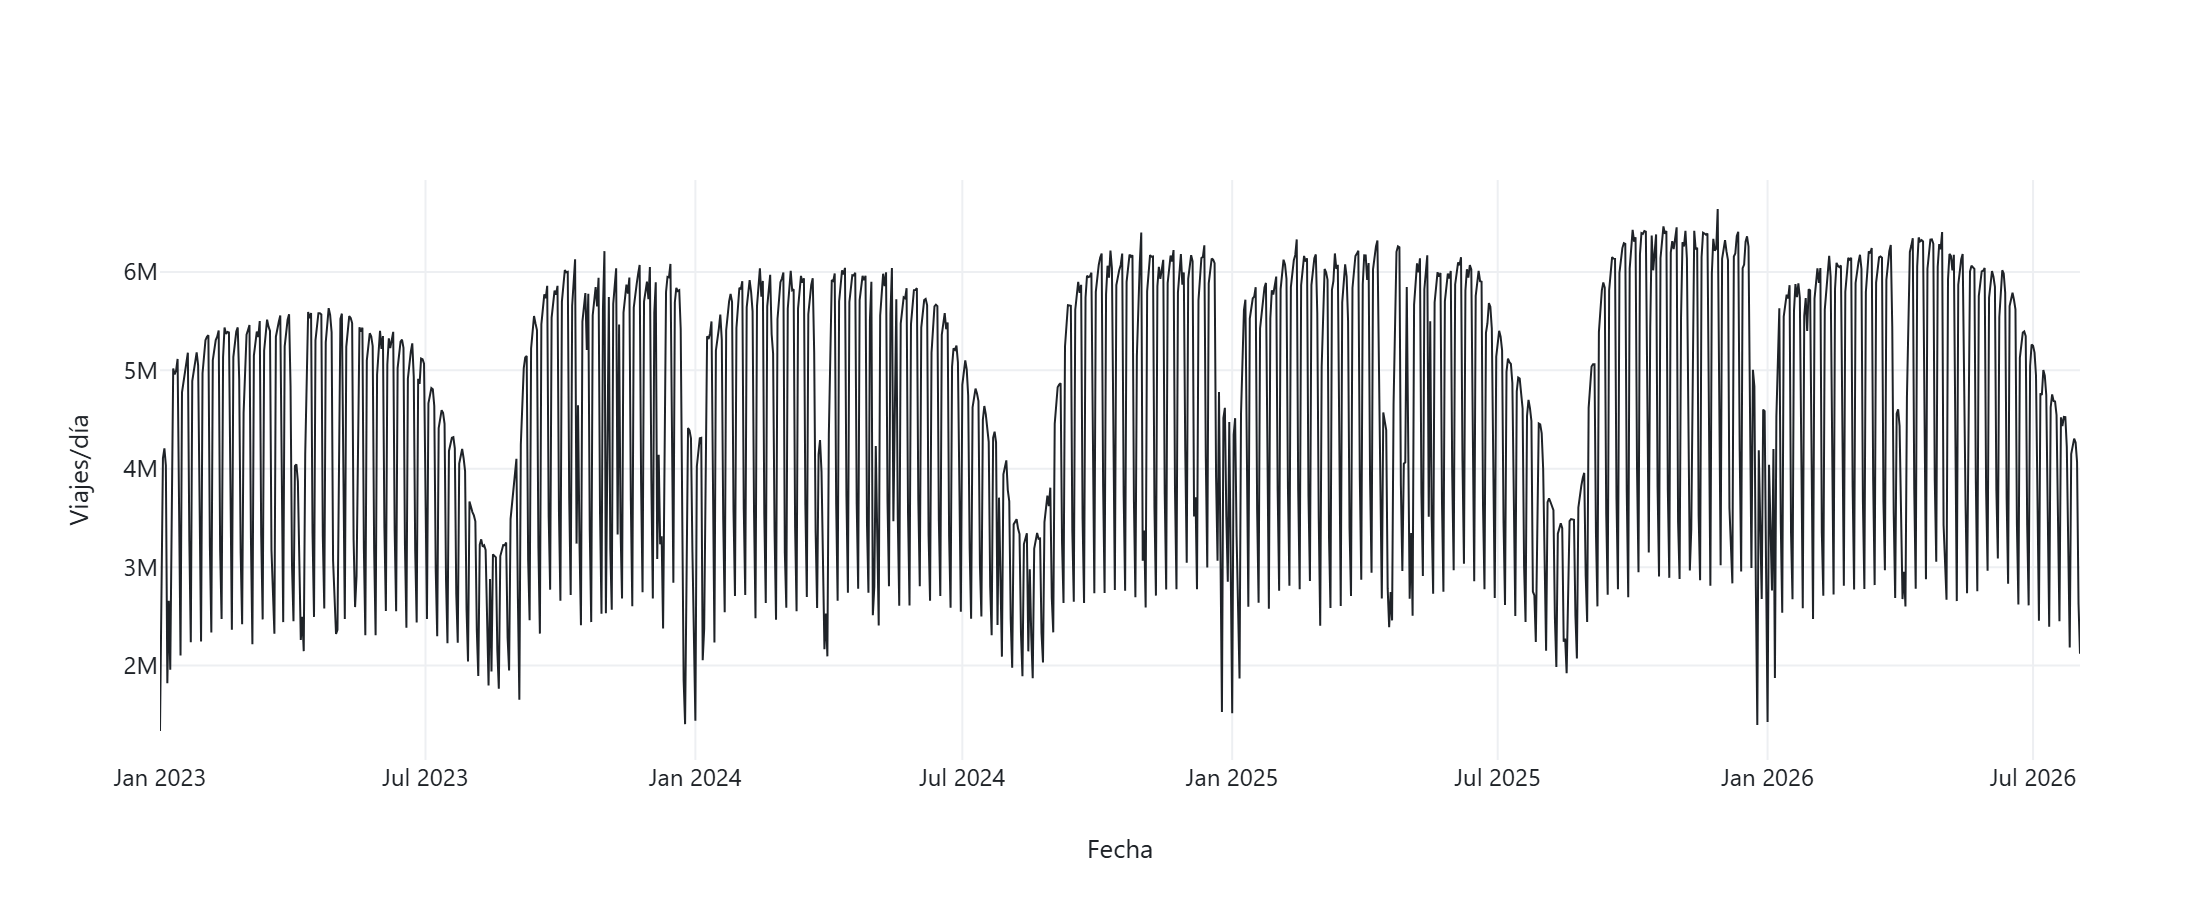
\includegraphics[width=0.78\textwidth]{fig_serie_completa_total.png}
  \caption{\headlinecolor{Demanda diaria total de transporte público en Madrid, serie completa.}}
  \label{fig:serie_completa_total}
\end{figure}

\section{Unificación y validación}\label{sec:unificacion_validacion}

Las tres fuentes se combinan mediante una unión interna (\emph{inner join}) sobre la
columna de fecha. Se prefiere a una unión externa por la izquierda porque esta fabricaría
filas exógenas enteramente nulas allí donde una fuente tuviera un hueco, contaminando
artificialmente el indicador de calidad ``cero nulos'' del conjunto unificado. La
contrapartida es que una unión interna oculta, por construcción, cualquier hueco de
cobertura: si una fecha faltara simultáneamente en las tres fuentes, el problema no se
manifestaría como una fila nula sino como una fila que no llega a existir. Por ello la
unificación aplica cuatro comprobaciones de integridad temporal en cadena: fechas
duplicadas dentro de cada fuente, antes de fusionar nada; el número de filas resultante
contra el de \emph{cada} fuente por separado, interrumpiendo la ejecución ante cualquier
discrepancia y señalando explícitamente las fechas concretas que se perderían, en lugar de
un recuento agregado; una reindexación del resultado contra un rango de fechas diario
completo entre el mínimo y el máximo observados, única comprobación capaz de detectar un
hueco común a las tres fuentes simultáneamente, precisamente el caso que la comparación
anterior no puede ver; y una verificación final de ausencia de duplicados y de valores
nulos sobre el conjunto ya unificado.

Las cuatro se someten además a pruebas negativas que inyectan huecos sintéticos en
conjuntos de datos de prueba en memoria y confirman que cada una interrumpe la ejecución
cuando corresponde, de manera que no puedan degradarse silenciosamente en verificaciones
inertes con el tiempo.

El resultado se persiste en \texttt{data/\allowbreak{}interim/\allowbreak{}unified\_daily.parquet} como una tabla
de 1.310 filas por 31 columnas, resumidas por grupos temáticos en la tabla
\ref{tab:esquema_unificado}: la fecha, las cinco columnas de demanda (el objetivo
\texttt{total} y los cuatro operadores), las veintiuna variables meteorológicas y las
cuatro columnas de calendario. Sobre ella se verifica, y se mantiene como invariante
durante todo el proyecto, que la suma de las cuatro columnas de operador reproduce
exactamente \texttt{total} en las 1.310 filas, salvo por una tolerancia de $10^{-6}$ que
absorbe el ruido de redondeo de las fórmulas de Excel del fichero de origen (por ejemplo,
un valor de \texttt{carretera} igual a $847904{,}00000001$ en la fila del 7 de julio de
2026, con una desviación del orden de $10^{-8}$ respecto al entero esperado); cualquier
desviación genuinamente fraccionaria, por encima de esa tolerancia, se trata como un error
de datos y detiene el proceso, ya que ensancharla para acallar un futuro fallo eliminaría
la capacidad de detectar una ruptura real de esa identidad.

Por último, los nulos que el calendario de origen deja en \texttt{holiday\_type} y
\texttt{holiday\_name} para los días sin festividad se sustituyen deliberadamente por el
centinela \texttt{'none'}: así la invariante de ``cero nulos'' conserva su significado
—cualquier nulo que aparezca en adelante señala un defecto real, no la ausencia ordinaria
de festividad— y la ingeniería de características recibe un nivel categórico limpio en
lugar de un hueco que codificar de forma ad hoc.

\begin{table}[htbp]
  \centering
  \small
  \begin{tabular}{>{\raggedright\arraybackslash}p{3.0cm}>{\centering\arraybackslash}p{2.0cm}>{\raggedright\arraybackslash}p{9.0cm}}
\toprule
\rowcolor{naranja}
\textbf{Grupo} & \textbf{N.º columnas} & \textbf{Ejemplo} \\
\midrule
\rowcolor{filaclara} Fecha & 1 & date \\
Demanda (target + operadores) & 5 & total, metro, emt, carretera, cercanias \\
\rowcolor{filaclara} Meteorología & 21 & temperature\_\allowbreak{}2m\_\allowbreak{}mean, precipitation\_\allowbreak{}sum, wind\_\allowbreak{}speed\_\allowbreak{}10m\_\allowbreak{}max \\
Calendario & 4 & day\_\allowbreak{}of\_\allowbreak{}week\_\allowbreak{}es, day\_\allowbreak{}type, holiday\_\allowbreak{}type, holiday\_\allowbreak{}name \\
\bottomrule
\end{tabular}

  \caption{\headlinecolor{Esquema unificado (\texttt{data/\allowbreak{}interim/\allowbreak{}unified\_daily.parquet}), 1.310 x 31.}}
  \label{tab:esquema_unificado}
\end{table}

La figura \ref{fig:demanda_por_operador} descompone la serie total por operador y hace
visible su jerarquía de escala: Metro de Madrid concentra el volumen mayor, seguido de
EMT, mientras que las concesionarias por carretera y Renfe Cercanías aportan magnitudes
sensiblemente menores pero con una textura semanal igualmente marcada. No participa en el
modelado del capítulo \ref{cap:metodologia}, cuyo único objetivo es \texttt{total}, pero
justifica que las cuatro columnas de operador se conserven íntegras a través de todo el
pipeline: son la base de este análisis exploratorio secundario y quedan disponibles para
un trabajo futuro de predicción desagregada por modo.

\begin{figure}[htbp]
  \centering
  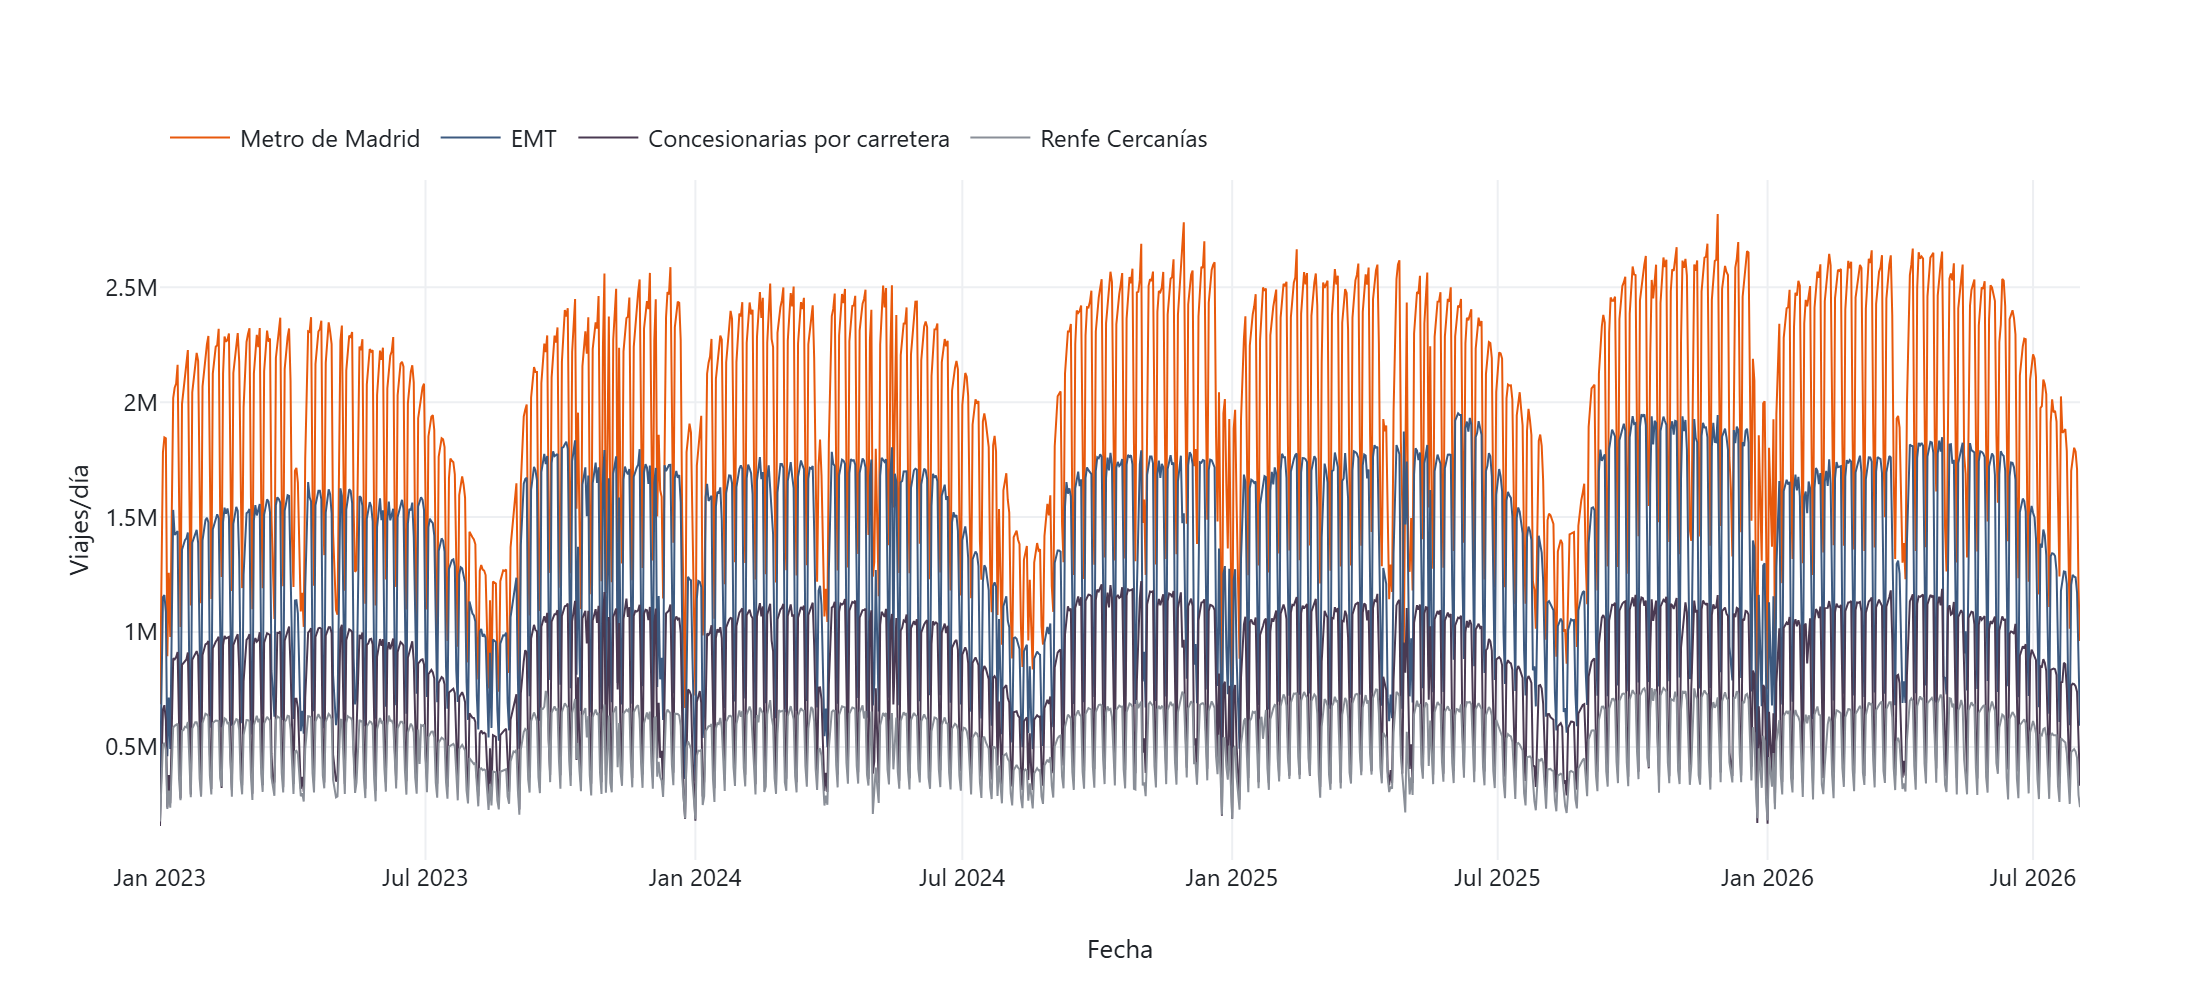
\includegraphics[width=0.78\textwidth]{fig_demanda_por_operador.png}
  \caption{\headlinecolor{Demanda diaria por operador del CRTM (Metro, EMT, carretera, Cercanías).}}
  \label{fig:demanda_por_operador}
\end{figure}

\section{Análisis exploratorio de datos}\label{sec:eda}

El análisis exploratorio persigue un objetivo acotado: caracterizar la estructura de
estacionalidad y de dispersión de la demanda antes de diseñar sobre ella la ingeniería de
características de la sección \ref{sec:ingenieria_features}, no agotar todas las lecturas
posibles de los datos. La serie completa (figura \ref{fig:serie_completa_total}) ya deja
ver, a simple vista y de forma repetida en cada uno de los tres años y medio cubiertos,
dos regularidades anuales: un desplome pronunciado y sostenido en agosto —el periodo
vacacional de mayor intensidad en Madrid, en el que se suspende buena parte de la
actividad laboral y educativa que sostiene la demanda de días laborables— y una
recuperación progresiva en septiembre que culmina en un máximo relativo hacia octubre y
noviembre, una vez restablecida por completo la actividad laboral y escolar.

La figura \ref{fig:estacionalidad_anual} lo cuantifica: la demanda media de agosto ronda
los 3 millones de viajes diarios, sensiblemente por debajo de cualquier otro mes, mientras
que octubre alcanza el máximo anual con una media próxima a los 5,2 millones; invierno y
primavera se mantienen en una meseta intermedia, entre 4,5 y 5 millones, con una
dispersión (barras de error de desviación típica) sistemáticamente mayor en los meses que
combinan más irregularidades de calendario —festivos nacionales y autonómicos, semana de
Navidad, Semana Santa de fecha variable— que en los meses centrales del curso.

\begin{figure}[htbp]
  \centering
  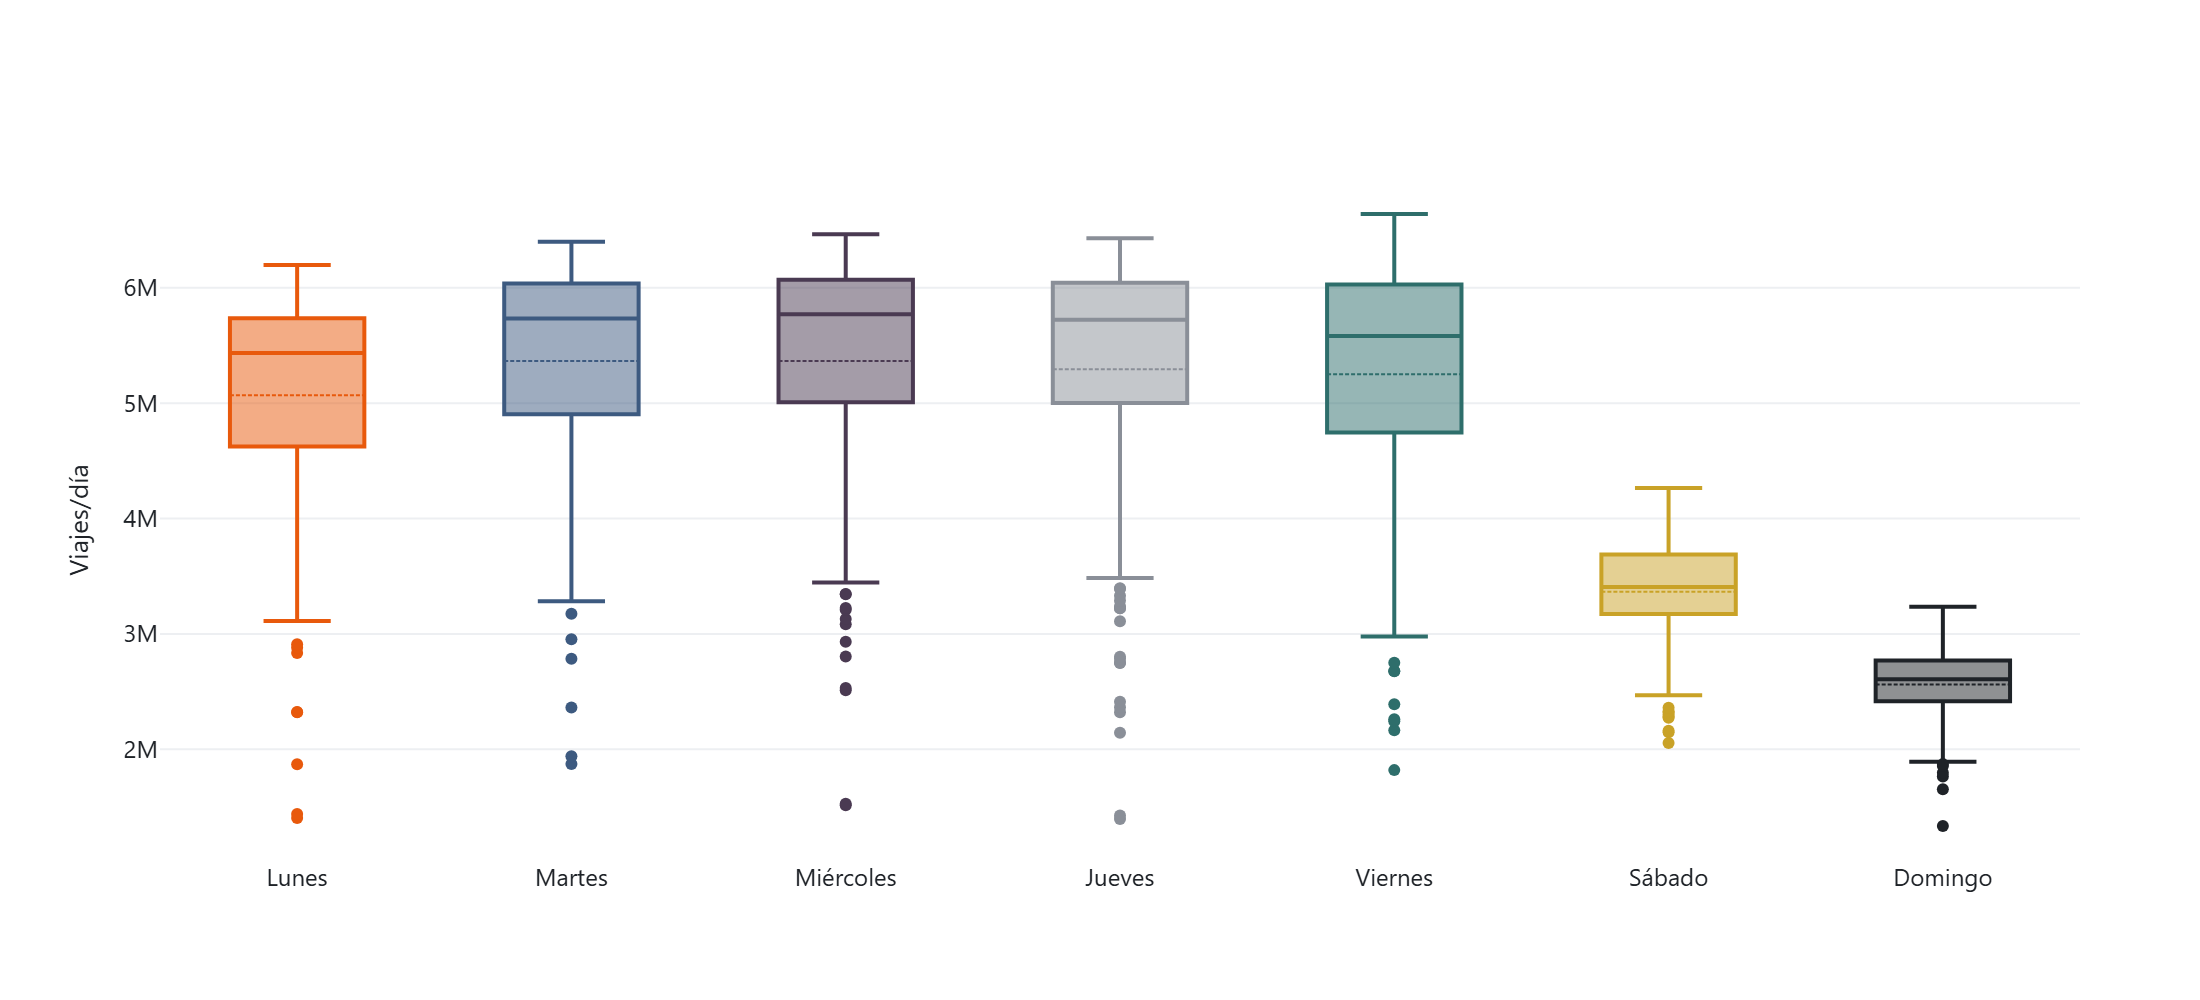
\includegraphics[width=0.78\textwidth]{fig_estacionalidad_semanal.png}
  \caption{\headlinecolor{Estacionalidad semanal de la demanda total (diagrama de caja por día de la semana).}}
  \label{fig:estacionalidad_semanal}
\end{figure}

La segunda regularidad, de periodicidad semanal y de magnitud mayor que la anual, está en
la figura \ref{fig:estacionalidad_semanal}. Los cinco días laborables presentan medianas
muy próximas entre sí, entre 5 y 5,5 millones de viajes diarios, con una cola inferior de
valores atípicos que corresponde a los festivos caídos en día laborable; el sábado
desciende a una mediana cercana a los 3,4 millones y el domingo, el día de menor demanda,
se sitúa alrededor de los 2,6 millones. La transición entre régimen laborable y fin de
semana implica, por tanto, un salto de aproximadamente 2,5 millones de viajes diarios dos
veces por semana, magnitud clave para interpretar correctamente los baselines del capítulo
\ref{cap:metodologia}: un modelo de persistencia ingenuo ($\hat y_t = y_{t-1}$) queda
sistemáticamente mal calibrado en cada transición viernes-sábado y domingo-lunes,
precisamente porque ignora esta estructura semanal tan pronunciada.

\begin{figure}[htbp]
  \centering
  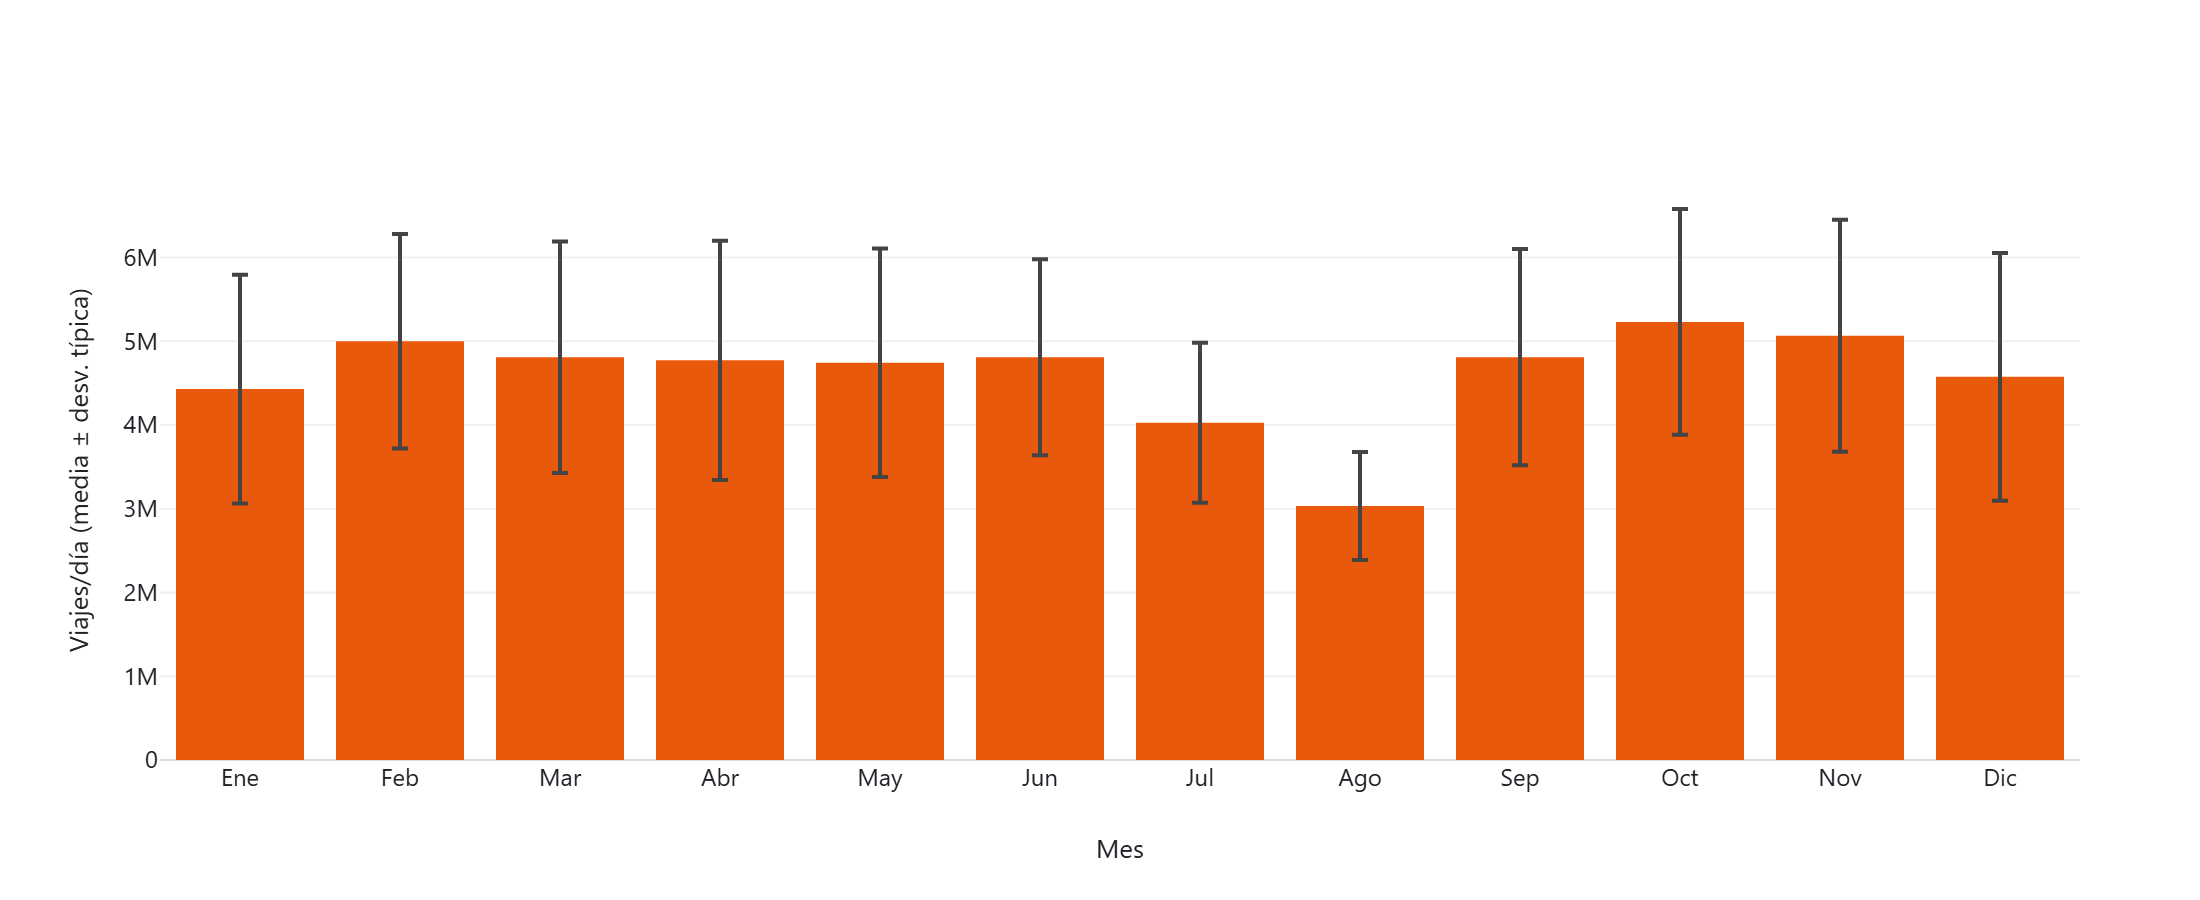
\includegraphics[width=0.78\textwidth]{fig_estacionalidad_anual.png}
  \caption{\headlinecolor{Estacionalidad anual de la demanda total (media mensual, 2023-2026).}}
  \label{fig:estacionalidad_anual}
\end{figure}

Por último, la figura \ref{fig:meteo_vs_demanda} cruza la demanda total con la
temperatura media diaria, coloreando cada observación por tipo de día. Es informativa
precisamente por lo que no muestra: dentro de cada franja de tipo de día la nube de puntos
se mantiene aproximadamente horizontal, sin una relación monótona clara entre temperatura
y demanda, mientras que la separación vertical entre franjas (laborable frente a sábado,
domingo y festivo) domina visualmente el gráfico. Sugiere que el \textbf{calendario, no la
meteorología, es el factor exógeno de primer orden} sobre la demanda agregada, y que la
meteorología, si aporta señal, lo hace como efecto secundario que matiza el nivel de cada
régimen de calendario más que como determinante independiente. Esta lectura motiva la
decisión, desarrollada en la sección \ref{sec:promocion_meteo}, de incorporar la
meteorología como bloque de variables exógenas retardadas y nunca como sustituto del
calendario.

\begin{figure}[htbp]
  \centering
  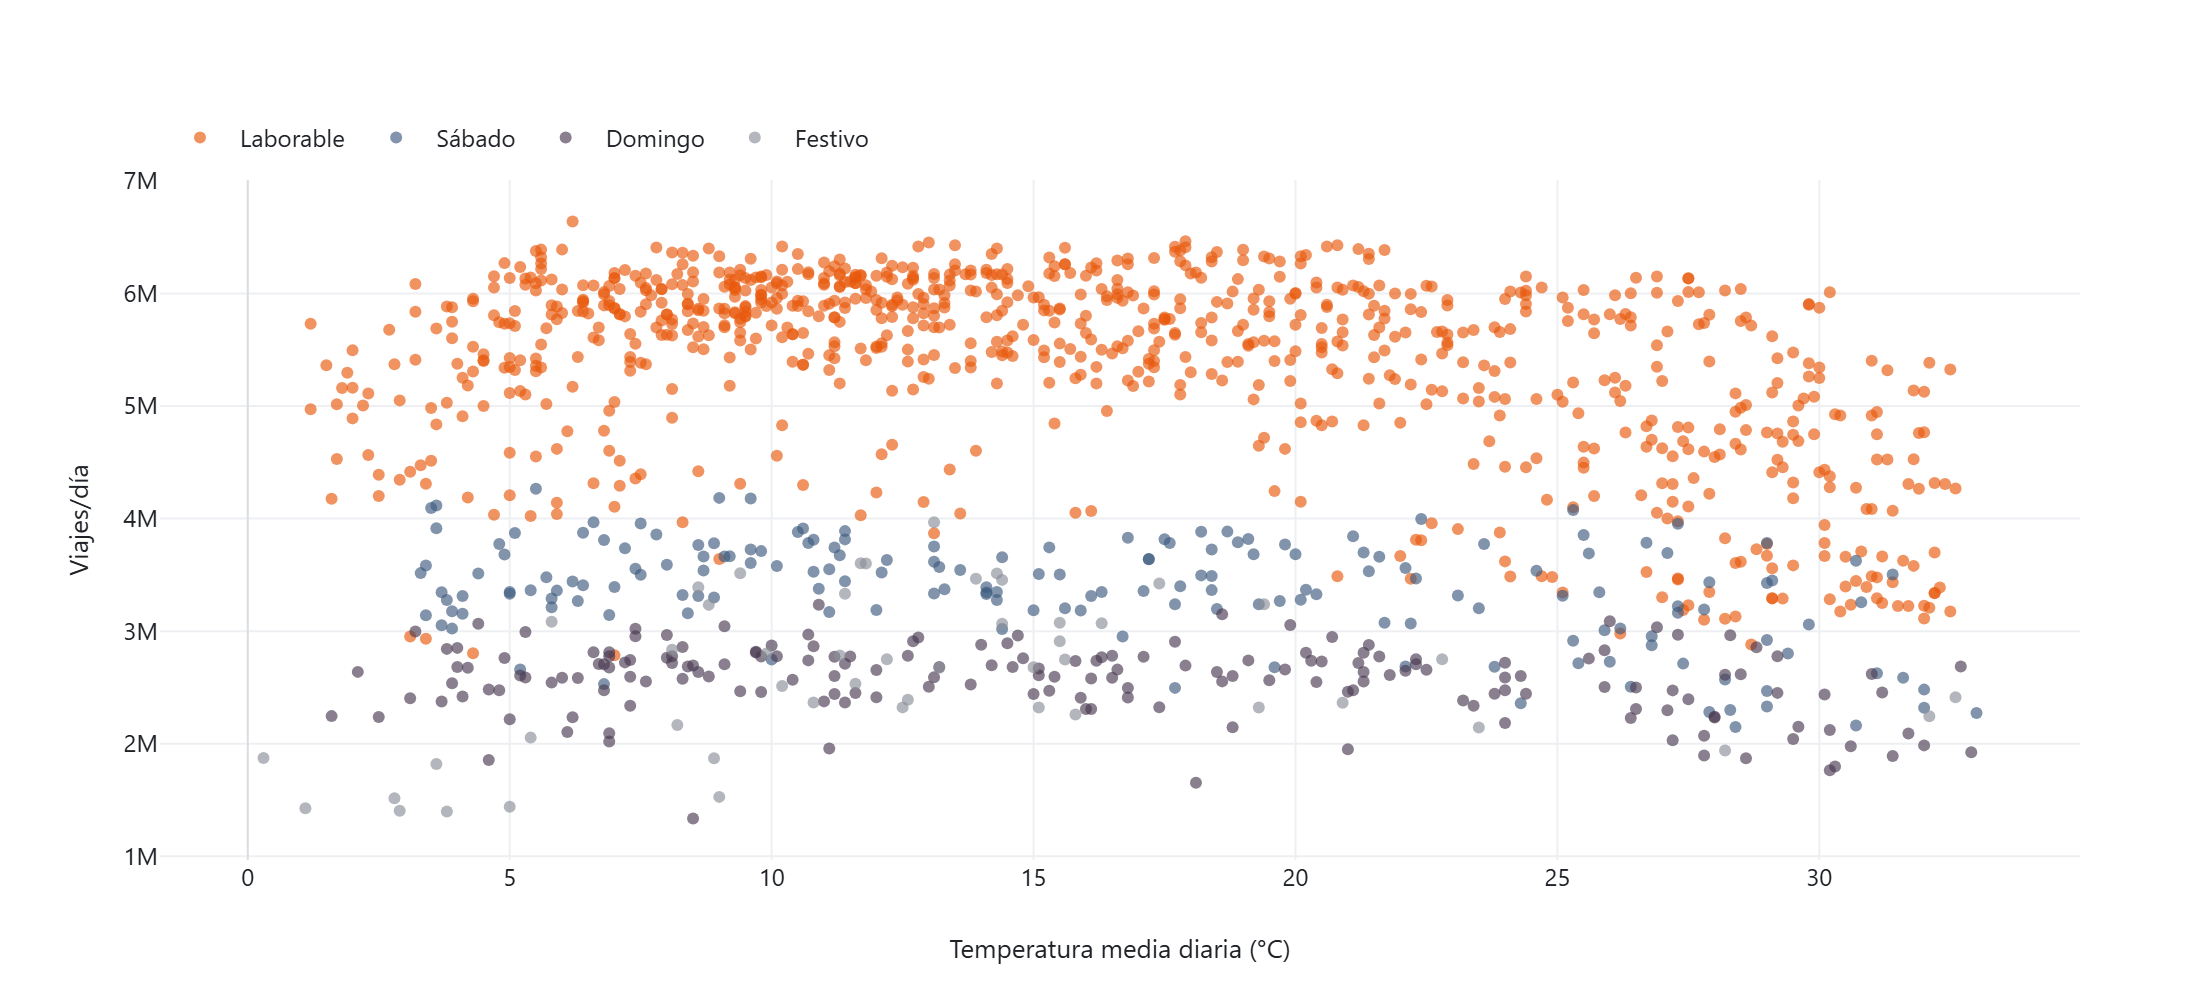
\includegraphics[width=0.78\textwidth]{fig_meteo_vs_demanda.png}
  \caption{\headlinecolor{Demanda total frente a temperatura media diaria, por tipo de día (EDA; la meteorología del mismo día no entra en el modelo).}}
  \label{fig:meteo_vs_demanda}
\end{figure}

\section{Ingeniería de características}\label{sec:ingenieria_features}

A partir del esquema unificado de la sección \ref{sec:unificacion_validacion} se
construye una matriz de 161 variables de modelado, todas identificadas por el prefijo
\texttt{feat\_} y recuperables mecánicamente mediante \texttt{feature\_columns()} en lugar
de una lista mantenida a mano. Es una decisión deliberada para que el conjunto de
variables no pueda derivar silenciosamente respecto del código que las genera. La tabla
\ref{tab:grupos_features} resume los seis grupos resultantes, cuyo diseño matemático se
detalla a continuación.

El primer grupo son los retardos de la propia demanda total,
$\text{lag}_k(\mathit{total})_t = \mathit{total}_{t-k}$ para
$k \in \{1, 2, 3, 7, 14, 21, 28\}$: siete variables que cubren desde la inercia de un día
para otro hasta la memoria calendario de cuatro semanas, elegida porque el retardo 28
recoge el mismo día de la semana cuatro veces atrás, bajo el mismo régimen semanal que la
sección \ref{sec:eda} identificó como dominante. El mismo esquema se aplica a cada columna
de operador, 28 variables más: el reparto modal de ayer es información legítimamente
disponible en el momento de la predicción y conserva señal real, a diferencia del reparto
modal del propio día que se discute más abajo. Se suman cuatro estadísticos móviles de la
demanda total (media y desviación típica sobre ventanas de 7 y 28 días) y seis términos de
Fourier deterministas que codifican la estacionalidad semanal ($k=1$) y anual ($k=1$ y
$k=2$) mediante pares seno-coseno:
\[
  \sin\!\left(\frac{2\pi k t}{T}\right), \qquad
  \cos\!\left(\frac{2\pi k t}{T}\right),
\]
con $T=7$ para el término semanal y $T=365{,}25$ para los anuales, y $t$ medido en días
desde una época fija, \texttt{FOURIER\_EPOCH = 2023-01-01}, deliberadamente distinta de la
fecha mínima observada en cada ejecución: fijarla evita que la llegada de datos futuros
modifique retroactivamente la codificación de una fecha ya existente.

El último grupo interno, de once variables, cubre el calendario mediante codificación
binaria exhaustiva (\emph{one-hot encoding}) del tipo de día y del tipo de festividad,
incluyendo explícitamente el nivel centinela \texttt{'none'} y la categoría de cero
observaciones \texttt{domingo festivo}, de modo que una fila con todo ceros sería un error
de codificación detectable y no una ambigüedad entre ``categoría base'' y ``fallo
silencioso''. Se añaden un indicador binario de fin de semana y uno de ``día puente'': un
día laborable inmediatamente anterior o posterior a un festivo o domingo festivo,
construido observando también el calendario del día siguiente. Esta mirada hacia adelante
no constituye fuga de información porque el calendario oficial de festivos español se
conoce con más de un año de antelación y es, por tanto, dato disponible en el momento de
la predicción; el procedimiento detectó 55 días puente en todo el periodo, todos
laborables por definición.

\begin{table}[htbp]
  \centering
  \small
  \begin{tabular}{>{\raggedright\arraybackslash}p{4.3cm}>{\centering\arraybackslash}p{2.0cm}>{\raggedright\arraybackslash}p{7.8cm}}
\toprule
\rowcolor{naranja}
\textbf{Grupo} & \textbf{N.º variables} & \textbf{Descripción} \\
\midrule
\rowcolor{filaclara} Retardos de la demanda total & 7 & lags 1, 2, 3, 7, 14, 21, 28 \\
Retardos de operadores & 28 & 4 operadores x 7 retardos \\
\rowcolor{filaclara} Medias/\allowbreak{}desv. móviles de la demanda & 4 & media y desv. típica, ventanas 7 y 28, shift-first \\
Términos de Fourier & 6 & semanal k=1, anual k=1 y k=2 \\
\rowcolor{filaclara} Calendario & 11 & day\_\allowbreak{}type (5), holiday\_\allowbreak{}type (4), is\_\allowbreak{}weekend, is\_\allowbreak{}bridge\_\allowbreak{}day \\
Meteorología retardada & 105 & 21 variables x (lags 1/\allowbreak{}2/\allowbreak{}3/\allowbreak{}7 + media móvil 7) \\
\rowcolor{filaclara} Total & 161 &  \\
\bottomrule
\end{tabular}

  \caption{\headlinecolor{Grupos de variables del modelo, 161 en total (\texttt{feature\_columns()}).}}
  \label{tab:grupos_features}
\end{table}

Dos reglas anti-fuga gobiernan la construcción de este bloque y se verifican mediante
pruebas automatizadas específicas. La primera exige que todo retardo o estadístico móvil
derivado de \texttt{total} o de una columna de operador aplique un desplazamiento de un
día, \texttt{shift(1)}, \emph{antes} de cualquier operación de ventana móvil: es decir,
$\text{roll}_w(s.\text{shift}(1))_t$ y nunca $\text{roll}_w(s)_t.\text{shift}(1)$ como
corrección a posteriori. Para una ventana móvil retrospectiva (\emph{trailing}) ambos
órdenes son matemáticamente equivalentes, de modo que la regla no corrige aquí ningún
error numérico observado; se exige de todos modos porque su corrección no depende de esa
equivalencia particular, que deja de cumplirse en cuanto la ventana se centra
(\texttt{center=True}), y porque una ventana sin desplazar en absoluto sí constituye una
fuga real y directa: la media móvil en el instante $t$ incorporaría el propio valor $y_t$
que se pretende predecir.

La segunda es un guardián de fuga contemporánea sobre las columnas de operador: puesto que
$\mathit{metro}_t + \mathit{emt}_t + \mathit{carretera}_t + \mathit{cercanias}_t =
\mathit{total}_t$ de forma exacta (sección \ref{sec:unificacion_validacion}), cualquier
columna de operador del \emph{mismo} día no es una variable predictiva, sino una
reformulación aritmética del propio objetivo, y su presencia en la matriz haría que un
modelo alcanzara un ajuste casi perfecto en entrenamiento para colapsar en inferencia,
momento en el que el reparto modal del día en curso no puede conocerse todavía. Se aplica
dos veces: sobre la salida de cada módulo de retardos y de nuevo sobre el fichero final
ensamblado, que es el punto donde una columna mal etiquetada terminaría incorporándose a
la matriz.

Conviene decir con precisión qué se calcula antes de la partición y por qué es seguro.
Las 161 variables se construyen sobre las 1.310 filas completas, antes de que actúe
ninguna función de partición (\texttt{build\_features} precede a
\texttt{chronological\_split} en todos los flujos). No introduce fuga porque todas son
\emph{causales}: el valor de cualquier retardo, estadístico móvil desplazado o variable
meteorológica retardada en la fila $t$ depende únicamente de filas estrictamente
anteriores a $t$, y ninguna estima parámetro alguno a partir de los datos (una media móvil
desplazada es una función fija de sus $w$ valores previos, no un estadístico ajustado
sobre la serie). Los términos de Fourier y las variables de calendario son, además,
funciones cerradas de la fecha que no observan el objetivo en ningún momento. Calcular
cualquiera de estas variables sobre el rango completo es, por tanto, idéntico fila a fila
a calcularla por separado dentro de cada partición. La única transformación que sí se
\emph{ajusta} sobre datos es el escalador \texttt{MinMaxScaler} de la etapa 1, y se ajusta
exclusivamente sobre el bloque de entrenamiento, y dentro de cada fold del esquema OOF
sobre la porción de entrenamiento de ese fold (sección \ref{sec:esquema_oof}).

\subsection{Promoción meteorológica: solo variables retardadas}\label{sec:promocion_meteo}

La sección \ref{sec:eda} dejó abierta, más que resuelta, la pregunta de si la
meteorología debía incorporarse a la matriz observada en tiempo real o bajo alguna forma
de retardo. Este proyecto la resuelve de manera conservadora: las 21 variables
meteorológicas del esquema unificado se promocionan a variables de modelado exclusivamente
en forma retardada, combinando los retardos de 1, 2, 3 y 7 días con una media móvil de 7
días (también construida con desplazamiento previo, por la misma regla anti-fuga de la
sección anterior), lo que produce $21 \times 5 = 105$ variables nuevas y eleva la matriz
de 56 a 161 columnas. La meteorología del propio día de la predicción no entra nunca en el modelo, ni siquiera
junto a las retardadas, y la prohibición se verifica mediante un guardián dedicado
(\texttt{\_assert\_no\_same\_day\_weather}) que se reejecuta sobre el conjunto final
ensamblado. La razón es que la meteorología observada del mismo día no es, en rigor, un
dato disponible en el momento operativo de la predicción, sino una observación posterior a
esta; usarla sin retardo equivaldría a asumir de forma implícita un pronóstico
meteorológico perfecto, un sesgo optimista que además se concentraría precisamente en los
días atípicos (temporales, olas de calor) en los que un pronóstico real es menos fiable y
en los que el efecto sobre la demanda sería, presumiblemente, mayor.

El conjunto de retardos elegido para la meteorología, $\{1, 2, 3, 7\}$, es
deliberadamente más corto que el de la demanda total, $\{1, 2, 3, 7, 14, 21, 28\}$, porque
ambas series obedecen a mecanismos de memoria distintos: la autocorrelación de la demanda
a 28 días está gobernada por el calendario (el mismo día de la semana, cuatro semanas
atrás, bajo un régimen semanal recurrente), mientras que la autocorrelación atmosférica
carece de un mecanismo equivalente y decae en la práctica a lo largo de una escala
sinóptica de tres a siete días; extender los retardos meteorológicos a 14, 21 o 28 días
habría añadido 63 columnas prácticamente redundantes con los términos de Fourier anuales,
que ya capturan de forma más limpia la componente puramente estacional del clima. Queda como línea pendiente, y explícitamente fuera del alcance de los resultados
principales de este TFM (\ref{sec:limitaciones}), una variante de sensibilidad con
meteorología del mismo día sin retardar, que solo tendría sentido reportar como cota
superior bajo el supuesto idealizado de un pronóstico meteorológico perfecto, y nunca
como modelo de referencia.

\section{Particiones y fuga de datos}\label{sec:particiones_fuga}

Todos los modelos de los capítulos \ref{cap:metodologia} y \ref{cap:resultados}
(baselines estadísticos, LSTM, XGBoost y sus combinaciones) comparten una única partición
cronológica 70/15/15, calculada por una sola función, \texttt{chronological\_split}, que
actúa como fuente única de verdad: ningún modelo recalcula sus propias fronteras
temporales, precisamente para que un desacuerdo de un solo día entre dos modelos sobre
dónde empieza el test no pueda invalidar silenciosamente su comparación. La partición
resultante, resumida en la tabla \ref{tab:particiones}, reserva 917 días (70,0\,\%) para
entrenamiento, desde el 1 de enero de 2023 hasta el 5 de julio de 2025; 196 días
(15,0\,\%) para validación, hasta el 17 de enero de 2026; y 197 días (15,0\,\%) para test,
hasta el final de la serie disponible, el 2 de agosto de 2026.

El cálculo de estas fronteras exige dos precauciones que, de omitirse, introducirían
errores sutiles y difíciles de detectar a posteriori. La primera es numérica: $0{,}70
\times 1310$ evalúa en aritmética de punto flotante a $916{,}9999\ldots$ (esto es,
$916{,}\overline{9}$ hasta la precisión de la máquina), de modo que un truncamiento
ingenuo mediante \texttt{int()} daría 916 días de entrenamiento en lugar de los 917 que
resultan de $\lfloor 0{,}70 \times 1310 \rfloor$; la implementación añade una tolerancia
$\varepsilon = 10^{-9}$ antes de truncar, precisamente para blindarse frente a ese error
de redondeo binario. La segunda es de diseño: las fronteras se resuelven sobre fracciones
acumuladas ($\lfloor 0{,}70 \, n \rfloor$ para el final de entrenamiento, $\lfloor 0{,}85
\, n \rfloor$ para el de validación) en lugar de aplicar el porcentaje de forma
independiente a cada partición, de modo que los tres bloques encajen exactamente, sin
solapamientos ni huecos de un día que un redondeo partición por partición sí podría
introducir.

\begin{table}[htbp]
  \centering
  \small
  \begin{tabular}{lllrr}
\toprule
\rowcolor{naranja}
\textbf{Partición} & \textbf{Inicio} & \textbf{Fin} & \textbf{Días} & \textbf{Porcentaje} \\
\midrule
\rowcolor{filaclara} Train & 2023-01-01 & 2025-07-05 & 917 & 70,0 \\
Val & 2025-07-06 & 2026-01-17 & 196 & 15,0 \\
\rowcolor{filaclara} Test & 2026-01-18 & 2026-08-02 & 197 & 15,0 \\
\bottomrule
\end{tabular}

  \caption{\headlinecolor{Partición cronológica 70/15/15 (\texttt{src.utils.splits.chronological\_split}).}}
  \label{tab:particiones}
\end{table}

Sobre esta partición actúa, además, una política de calentamiento (\emph{warm-up})
derivada de la ingeniería de características de la sección \ref{sec:ingenieria_features}:
las 28 primeras filas de entrenamiento (2023-01-01 a 2023-01-28) contienen nulos en las
variables que dependen del retardo o la ventana móvil más larga, 28 días, y se descartan,
reduciéndolo de 917 a 889 filas efectivas; validación y test, muy por delante de esa
ventana inicial, no se ven afectados y conservan sus 196 y 197 días íntegros. La aplica
\texttt{apply\_warmup\_policy}, que \emph{interrumpe} la ejecución si el calentamiento
necesario llegara a alcanzar validación o test, en lugar de recortar silenciosamente el
periodo de evaluación: un conjunto de evaluación acortado sin aviso produciría métricas
que dejarían de ser comparables entre modelos y entre reejecuciones del pipeline, un
riesgo que se considera preferible convertir en un fallo explícito y temprano.


\chapter{Arquitectura híbrida residual LSTM-XGBoost para demanda diaria agregada}\label{cap:metodologia}

Este capítulo describe la arquitectura de modelado propuesta y el protocolo experimental
que la sustenta, sobre la matriz de 161 variables construida en el capítulo
\ref{cap:datos_features}. La propuesta central es un híbrido residual secuencial de dos
etapas: una red LSTM univariante (etapa 1) que modela la dinámica temporal de la propia
demanda, y un modelo XGBoost (etapa 2) que corrige, a partir de la matriz completa de
variables predictoras (calendario y meteorología retardada, pero también retardos y
estadísticos móviles de la propia demanda), el residuo que la etapa 1 deja sin explicar.
Formalmente, si
$\hat y^{\text{LSTM}}_t$ denota la predicción de la etapa 1 en el instante $t$, el residuo
que alimenta la etapa 2 se define como
\[
  e_t = y_t - \hat y^{\text{LSTM}}_t,
\]
y la predicción final del sistema combina ambas etapas por suma directa,
\[
  \hat y^{\text{final}}_t = \hat y^{\text{LSTM}}_t + \hat e^{\text{XGBoost}}_t .
\]

Conviene precisar en qué difiere este diseño del esquema híbrido ARIMA-red neuronal de
\textcite{zhang2003hybrid}, que es su referente más directo en la literatura y al que
se volverá al interpretar el resultado central del capítulo \ref{cap:resultados}
(\ref{sec:resultado_negativo_teoria}). En primer lugar, el orden de las etapas está
invertido: aquí es la red neuronal la que modela primero la componente no lineal de la
serie y un modelo basado en árboles el que corrige después, no al revés. En segundo
lugar, la etapa 2 de este TFM no modela el residuo como una serie temporal autorregresiva
sobre sus propios retardos, sino como una función de 161 variables predictoras (retardos
de la demanda, calendario, meteorología retardada, términos de Fourier) construidas de
forma independiente de la
dinámica del residuo mismo. Y en tercer lugar, y de manera no negociable para la validez
del diseño, las predicciones de la etapa 1 que se emplean para calcular ese residuo de
entrenamiento se generan siempre fuera de muestra (\emph{out-of-fold}, OOF), mediante un
esquema de validación cruzada expansivo hacia adelante (\ref{sec:esquema_oof}) y nunca a
partir de un único ajuste \emph{in-sample}: un residuo calculado sobre predicciones que el
propio modelo ya ha visto en entrenamiento está optimistamente sesgado hacia cero y es
estructuralmente distinto del residuo que la etapa 2 enfrentará realmente en inferencia,
de modo que aprender a corregirlo no transferiría a producción.

\section{Diagnóstico previo: ¿tiene el residuo estructura de calendario?}\label{sec:diagnostico_previo}

Antes de comprometerse con la arquitectura de dos etapas descrita más arriba conviene
comprobar, con evidencia y no por intuición, que existe una estructura de error
sistemática que una segunda etapa no lineal pueda efectivamente corregir: si un modelo
lineal ya captura todo el error explicable, ni el híbrido residual ni el repesado por
calendario de la sección \ref{sec:experimento_a} tendrían ningún margen de mejora
posible. Este diagnóstico exploratorio se calcula sobre el error absoluto de SARIMAX
(el baseline estadístico de la sección \ref{sec:baselines}, disponible ya en esta fase
del proyecto) agregado por régimen de calendario sobre las 1.282 observaciones
posteriores al recorte de calentamiento de 28 días (sección \ref{sec:particiones_fuga}),
y es deliberadamente exploratorio: se calcula sobre el periodo completo train+val+test
y no sobre una partición fuera de muestra, porque los días festivos son demasiado raros
(48 en total) para dividirlos de forma fiable en tres particiones y seguir teniendo un
tamaño de grupo interpretable.

El resultado confirma la premisa de la arquitectura híbrida: el error absoluto medio de
SARIMAX es 492.092 en festivos (20,50\,\% de error porcentual medio) y 262.194 en
sábado, frente a 212.383 en laborables en general, y el sesgo con signo es
sistemáticamente negativo en festivos ($-145.250$), es decir, SARIMAX
\textbf{sobreestima} la demanda festiva de forma consistente sin saber cuantificar
correctamente su magnitud.

El contraste más nítido, sin embargo, aísla el efecto de los
días puente del efecto de fin de semana comparando únicamente dentro del régimen
laborable: los 54 días laborables de tipo puente presentan un error absoluto medio de
518.634 frente a 192.191 en los 819 laborables ordinarios, es decir,
\textbf{los días puente concentran 2,70 veces el error absoluto medio de un laborable
corriente}. Esta es exactamente la estructura no lineal y condicionada al calendario
(grande en magnitud, concentrada en un subconjunto pequeño y bien identificable de
días) que la etapa 2 de la arquitectura híbrida (sección \ref{sec:etapa2_xgboost}) está
diseñada para aprender a partir de variables exógenas, y la que motiva directamente,
más adelante, tanto el repesado de días irregulares del experimento A (sección
\ref{sec:experimento_a}) como la lectura del desglose de error por tipo de día del
capítulo \ref{cap:resultados} (sección \ref{sec:error_dia}). Que el mecanismo exista de
forma medible en este diagnóstico exploratorio, y que aun así el híbrido resultante no
supere a sus componentes de una sola etapa, es precisamente el contraste que sostiene
el hallazgo central de este TFM: el problema no es que no haya señal de calendario que
corregir, sino que la etapa 1 de la que parte esa corrección es demasiado débil
(sección \ref{sec:resultado_negativo_teoria}).

\section{Baselines}\label{sec:baselines}

Antes de evaluar cualquier arquitectura de aprendizaje automático es necesario fijar la
referencia frente a la que se mide: un conjunto de modelos de referencia sencillos que
establezcan cuánta señal puede explicarse sin recurrir a redes neuronales ni a variables
exógenas. El primero, la persistencia $\hat y_t = y_{t-1}$, resulta ser un modelo de referencia
particularmente débil sobre esta serie: como se documentó en la sección \ref{sec:eda}, la
demanda salta en torno a 2,5 millones de viajes diarios en cada transición entre régimen
laborable y régimen de fin de semana, una transición que ocurre dos veces por semana, y la
persistencia ignora por construcción cualquier estructura de calendario. El resultado es
un coeficiente de determinación negativo tanto en entrenamiento como en test, lo que
indica que ni siquiera predecir la media de la serie sería peor. Por ello, el baseline
ingenuo relevante en este trabajo es la persistencia estacional $\hat y_t = y_{t-7}$, que
sí incorpora el ciclo semanal al comparar cada día con el mismo día de la semana anterior;
superar a la persistencia estacional, y no a la persistencia simple, es el umbral
que cualquier modelo posterior debe rebasar para justificar su complejidad adicional.

El baseline estadístico fuerte de esta familia es un modelo SARIMAX, seleccionado
mediante una búsqueda en rejilla de 324 combinaciones de órdenes
$(p,d,q)\times(P,D,Q,s)$, con $p,q,P,Q \in \{0,1,2\}$, $d,D \in \{0,1\}$ y periodo
estacional fijo $s=7$, el ciclo semanal identificado en el análisis exploratorio. La
selección se realiza exclusivamente por el criterio de información de Akaike (AIC)
calculado sobre el conjunto de entrenamiento, deliberadamente sin consultar en ningún
momento el error de validación: hacerlo convertiría la validación en un conjunto de
ajuste adicional y contaminaría la comparación que se plantea en el capítulo
\ref{cap:resultados}. El orden seleccionado, resumido en la tabla \ref{tab:sarimax_orden},
es $\text{SARIMAX}(2,1,2)\times(0,1,2,7)$, con un AIC de entrenamiento de 24.616,89; las
cinco combinaciones mejor puntuadas se sitúan dentro de 0,8 puntos de AIC entre sí, de
modo que el orden concreto elegido debe leerse como \emph{una} especificación razonable de
esta complejidad, no como una verdad estructural descubierta de forma inequívoca.

\begin{table}[htbp]
  \centering
  \small
  \begin{tabular}{llrr}
\toprule
\rowcolor{naranja}
\textbf{Orden (p,d,q)} & \textbf{Orden estacional (P,D,Q,s)} & \textbf{AIC} & \textbf{N.º variables exógenas} \\
\midrule
\rowcolor{filaclara} (2,1,2) & (0,1,2,7) & 24.616,89 & 5 \\
\bottomrule
\end{tabular}

  \caption{\headlinecolor{Orden SARIMAX seleccionado por AIC sobre 324 combinaciones.}}
  \label{tab:sarimax_orden}
\end{table}

El vector de variables exógenas se limita deliberadamente a cinco columnas de calendario
(los indicadores de fin de semana y de día puente, y las tres categorías reales de tipo
de festividad, excluyendo \texttt{feat\_holiday\_type\_none} como nivel de referencia para
evitar la trampa de la variable ficticia frente al intercepto de la regresión), sin
incorporar ningún retardo ni estadístico móvil de la propia demanda: el componente
$(p,d,q)\times(P,D,Q,s)$ del modelo ya captura la autorregresión y la diferenciación
estacional de la serie \parencite{box1970time}, y añadir retardos hechos a mano expresaría la
misma dependencia dos veces a través de dos mecanismos en competencia.

Los parámetros del modelo se estiman una única vez sobre el conjunto de entrenamiento; a partir de ahí, la
predicción sobre validación y test es un pronóstico \emph{walk-forward} de un paso
mediante el filtro de Kalman (\texttt{.filter()}, sin reestimación de parámetros) con
\texttt{get\_prediction(dynamic=False)}, de modo que cada predicción en el instante $t$
condiciona exclusivamente sobre las observaciones reales hasta $t-1$. La evaluación de
SARIMAX corresponde, por tanto, a un escenario de predicción \textbf{de un día hacia
adelante}, actualizado diariamente una vez conocida la demanda observada del día anterior;
no representa un pronóstico estático de todo el periodo de evaluación realizado desde su
fecha inicial. Se prefiere este
esquema a un único pronóstico estático a 390 días porque este último decaería hacia la
media de la serie y mediría, en la práctica, una distancia de extrapolación en lugar de la
calidad real del modelo; se verificó además que los residuos no presentan autocorrelación
de primer orden relevante (aproximadamente $-0{,}03$) y que la predicción sigue de cerca
el valor real del propio día ($\text{MAE}=163.627$) y no el del día anterior
($\text{MAE}=909.082$), descartando así un desfase temporal accidental en la
implementación. Con este protocolo, SARIMAX alcanza un MAPE de test del 3,85\,\% y un
$R^2$ de 0,9672 (tabla \ref{tab:comparacion_test}, sección \ref{sec:tabla_maestra}),
constituyéndose en un baseline exigente que cualquier arquitectura de aprendizaje
automático de este TFM debe superar para justificar su mayor coste de desarrollo. Es el
mismo horizonte de un día al que se evalúan todos los demás modelos del estudio: la matriz
de variables solo contiene retardos $\geq 1$ y la ventana de la etapa 1 abarca $[t-W, t)$,
de modo que la comparación de la tabla maestra es entre pronósticos a un día vista en todos
los casos.

\section{Etapa 1: LSTM}\label{sec:etapa1_lstm}

La primera etapa del híbrido es una red LSTM \parencite{hochreiter1997lstm}
\textbf{univariante por diseño}: recibe únicamente la ventana de las $W$ observaciones
pasadas de \texttt{total} y debe inferir a partir de esa dinámica (sin ningún indicador de
día de la semana, festividad o puente) toda la estructura de calendario que la sección
\ref{sec:eda} mostró dominante. Esta restricción no es una limitación accidental, sino la
pregunta que la etapa 1 está diseñada para responder: cuánta de esa estructura puede
recuperarse de la memoria temporal de la serie por sí sola, dejando a la etapa 2 la tarea
explícita de aportar la información de calendario y meteorología que la etapa 1
estructuralmente no puede ver.

La longitud de la ventana $W$ se fijó mediante una comparación empírica, no una búsqueda
exhaustiva, entre tres valores candidatos, $W \in \{14, 28, 60\}$, entrenando en cada caso
un modelo final completo y evaluándolo únicamente sobre la partición de validación; el
conjunto de test se mantuvo deliberadamente fuera de esta decisión, de modo que la
elección de $W$ no pudiera beneficiarse, ni siquiera indirectamente, de información sobre
la partición de evaluación final. Los resultados se recogen en la tabla
\ref{tab:ventana_lstm}: $W=28$ resulta ganador en las cuatro métricas de validación
simultáneamente, con una brecha de MAE de aproximadamente el 11\,\% frente a sus dos
vecinos, una diferencia lo bastante amplia como para no atribuirse al azar de una única
ejecución, aunque el propio diseño del experimento, una ejecución por valor de $W$, obliga
a presentarla como evidencia documentada y no como el resultado de una búsqueda
sistemática de hiperparámetros.

\begin{table}[htbp]
  \centering
  \small
  \setlength{\tabcolsep}{4pt}
  \resizebox{\textwidth}{!}{%
    \begin{tabular}{>{\centering\arraybackslash}p{0.8cm}>{\centering\arraybackslash}p{2.1cm}>{\centering\arraybackslash}p{2.0cm}>{\centering\arraybackslash}p{1.7cm}>{\centering\arraybackslash}p{1.9cm}>{\centering\arraybackslash}p{1.9cm}>{\centering\arraybackslash}p{2.0cm}>{\centering\arraybackslash}p{1.5cm}}
\toprule
\rowcolor{naranja}
\textbf{W} & \textbf{Secuencias train} & \textbf{Épocas ejecutadas} & \textbf{Mejor época} & \textbf{MAE (val)} & \textbf{RMSE (val)} & \textbf{MAPE (val, \%)} & \textbf{R² (val)} \\
\midrule
\rowcolor{filaclara} 14 & 875 & 154 & 144 & 459.813 & 721.182 & 13,28 & 0,7607 \\
28 & 861 & 164 & 154 & 411.142 & 655.479 & 11,81 & 0,8023 \\
\rowcolor{filaclara} 60 & 829 & 87 & 77 & 456.063 & 692.825 & 12,89 & 0,7792 \\
\bottomrule
\end{tabular}
%
  }
  \caption{\headlinecolor{Comparación de longitud de ventana W (evidencia, no búsqueda exhaustiva: una ejecución final por W, test nunca consultado en la elección).}}
  \label{tab:ventana_lstm}
\end{table}

Conviene señalar que $W$ se eligió observando precisamente la
partición de validación: por tanto, las métricas de validación de toda la familia
LSTM (\texttt{lstm\_alone}, \texttt{hybrid}, \texttt{hybrid\_weighted}) son levemente
optimistas respecto de lo que cabría esperar de una evaluación totalmente independiente,
mientras que sus métricas de test, nunca consultadas durante esta elección, constituyen
la evaluación estrictamente limpia y son las que deben citarse como comparación
principal frente a SARIMAX y XGBoost.

La arquitectura final, entrenada sobre $W=28$, es deliberadamente compacta:
una capa LSTM de 32 unidades con desactivación aleatoria (\emph{dropout}) de 0,2, seguida de una capa densa de
salida lineal de una única neurona. Se optimiza con Adam ($\text{lr}=10^{-3}$) bajo error
cuadrático medio, en lotes de 32 secuencias, con parada anticipada de paciencia 10 y
restauración de los mejores pesos observados (\texttt{restore\_best\_weights}). El corte
de la parada anticipada se decide sobre una cola interna de las propias secuencias de
\emph{entrenamiento} (las últimas 129, correspondientes al periodo 2025-02-27 a
2025-07-05) y nunca sobre la partición de validación oficial: emplear la validación
oficial en ese punto convertiría la parada anticipada en un mecanismo de ajuste sobre
validación, sesgando de forma optimista y silenciosa cada cifra de validación que se
reporte más adelante en la tabla maestra de comparación (\ref{sec:tabla_maestra}).

Entrenada de este modo sobre las 889 filas de entrenamiento posteriores al calentamiento,
la etapa 1 en solitario queda claramente por debajo de SARIMAX en ambas particiones de
evaluación. Y, más revelador todavía, no llega a superar ni siquiera a la persistencia
estacional cuando ambas se comparan sobre las mismas filas fuera de muestra generadas por
el esquema de la sección \ref{sec:esquema_oof} (MAE OOF de 690.460 frente a 461.087).
Esto no constituye un defecto de la implementación: los resultados obtenidos indican
que la dinámica temporal univariante, por sí sola, no basta
para igualar a un modelo que sí observa el calendario de forma explícita. El detalle
numérico completo de esta comparación, junto con el resto de modelos de una sola etapa,
se presenta en la tabla maestra del capítulo \ref{cap:resultados}
(\ref{sec:tabla_maestra}).

Dos decisiones de ajuste, verificadas empíricamente y no asumidas de antemano, merecen
constar. Primero, el número máximo de épocas se elevó de 200 a 500 tras observar que el
fold 3 del esquema OOF alcanzaba las 200 épocas sin que la parada anticipada hubiera
actuado todavía —es decir, el límite artificial de épocas, no la convergencia del modelo,
era la restricción activa—, lo que habría entrenado folds de tamaño distinto hasta
presupuestos de cómputo efectivamente distintos y los habría hecho incomparables entre sí;
al elevar el límite, el fold 3 llegó a 228 épocas y su MAE mejoró de 288.194 a 282.122.
Segundo, se probó y se descartó el barajado de los lotes de entrenamiento: aunque barajar
secuencias ya construidas no constituiría en sí misma una fuga de información —cada
secuencia es autocontenida y la cola de parada anticipada se separa cronológicamente antes
de cualquier barajado—, medido sobre el fold 3 el barajado empeoró el resultado (MAE OOF de
288.000 a 309.000 aproximadamente), por lo que se mantiene \texttt{shuffle=False} por
evidencia, no por precaución teórica.

\section{Esquema de validación fuera de muestra (OOF)}\label{sec:esquema_oof}

El esquema descrito en esta sección es, con diferencia, el componente metodológico más
crítico del proyecto: la decisión de diseño de la que depende la validez de toda la etapa
2. Como se anticipó en la introducción del capítulo, las predicciones de la etapa 1 que
alimentan el cálculo del residuo de entrenamiento de la etapa 2 deben generarse siempre
fuera de muestra. La alternativa sería ajustar un único modelo LSTM sobre todo el
entrenamiento y calcular el residuo directamente sobre esas mismas predicciones
\emph{in-sample}, y produciría un residuo artificialmente pequeño y con una distribución
distinta de la que la etapa 2 encontrará en producción, precisamente porque el modelo ya
ha memorizado, en algún grado, las observaciones sobre las que se evalúa; la etapa 2
aprendería entonces a corregir una distribución de error que no existe fuera de muestra,
lo que se traduciría en un desempeño peor del esperado en inferencia real. Este esquema de
validación fuera de muestra para series temporales sigue la práctica establecida en la
literatura de evaluación de modelos de pronóstico
\parencite{bergmeir2012cv,cerqueira2020evaluating}, adaptada aquí a la generación de
predicciones de \emph{stacking} \parencite{wolpert1992stacking} en dos etapas.

Concretamente, se emplea una validación cruzada expansiva hacia adelante
(\emph{walk-forward}) de cinco folds sobre el periodo de entrenamiento posterior al
calentamiento, 2023-01-29 a 2025-07-05 (889 filas). El fold $k$ entrena un modelo LSTM
completo sobre el bloque $[0, s_k)$ y genera predicciones únicamente sobre el bloque
inmediatamente siguiente, $[s_k, s_{k+1})$, que nunca ha visto durante su entrenamiento;
cada fold reajusta además su propio escalador de normalización exclusivamente sobre su
propia porción de entrenamiento, sin reutilizar en ningún caso un escalador ajustado con
información de un bloque posterior. La tabla \ref{tab:folds_oof} recoge las métricas de
cada uno de los cinco folds, y la figura \ref{fig:oof_folds} muestra sus predicciones
fuera de muestra frente al valor real.

\begin{table}[htbp]
  \centering
  \small
  \setlength{\tabcolsep}{4pt}
  \resizebox{\textwidth}{!}{%
    \begin{tabular}{>{\centering\arraybackslash}p{1.0cm}>{\centering\arraybackslash}p{2.1cm}>{\centering\arraybackslash}p{1.9cm}>{\centering\arraybackslash}p{2.2cm}>{\centering\arraybackslash}p{2.1cm}>{\centering\arraybackslash}p{1.9cm}>{\centering\arraybackslash}p{1.9cm}}
\toprule
\rowcolor{naranja}
\textbf{Fold} & \textbf{Épocas ejecutadas} & \textbf{Mejor época} & \textbf{Loss train (final)} & \textbf{Loss val (final)} & \textbf{MAE} & \textbf{RMSE} \\
\midrule
\rowcolor{filaclara} 1 & 15 & 5 & 0,1195 & 0,0788 & 1.461.905 & 1.682.893 \\
2 & 153 & 143 & 0,0271 & 0,0509 & 659.425 & 882.524 \\
\rowcolor{filaclara} 3 & 228 & 218 & 0,0207 & 0,0281 & 282.122 & 397.512 \\
4 & 131 & 121 & 0,0208 & 0,0098 & 548.081 & 839.318 \\
\rowcolor{filaclara} 5 & 81 & 71 & 0,0251 & 0,0331 & 506.148 & 718.174 \\
\bottomrule
\end{tabular}
%
  }
  \caption{\headlinecolor{Métricas por fold del esquema OOF \emph{walk-forward} expansivo (5 folds).}}
  \label{tab:folds_oof}
\end{table}

\begin{figure}[htbp]
  \centering
  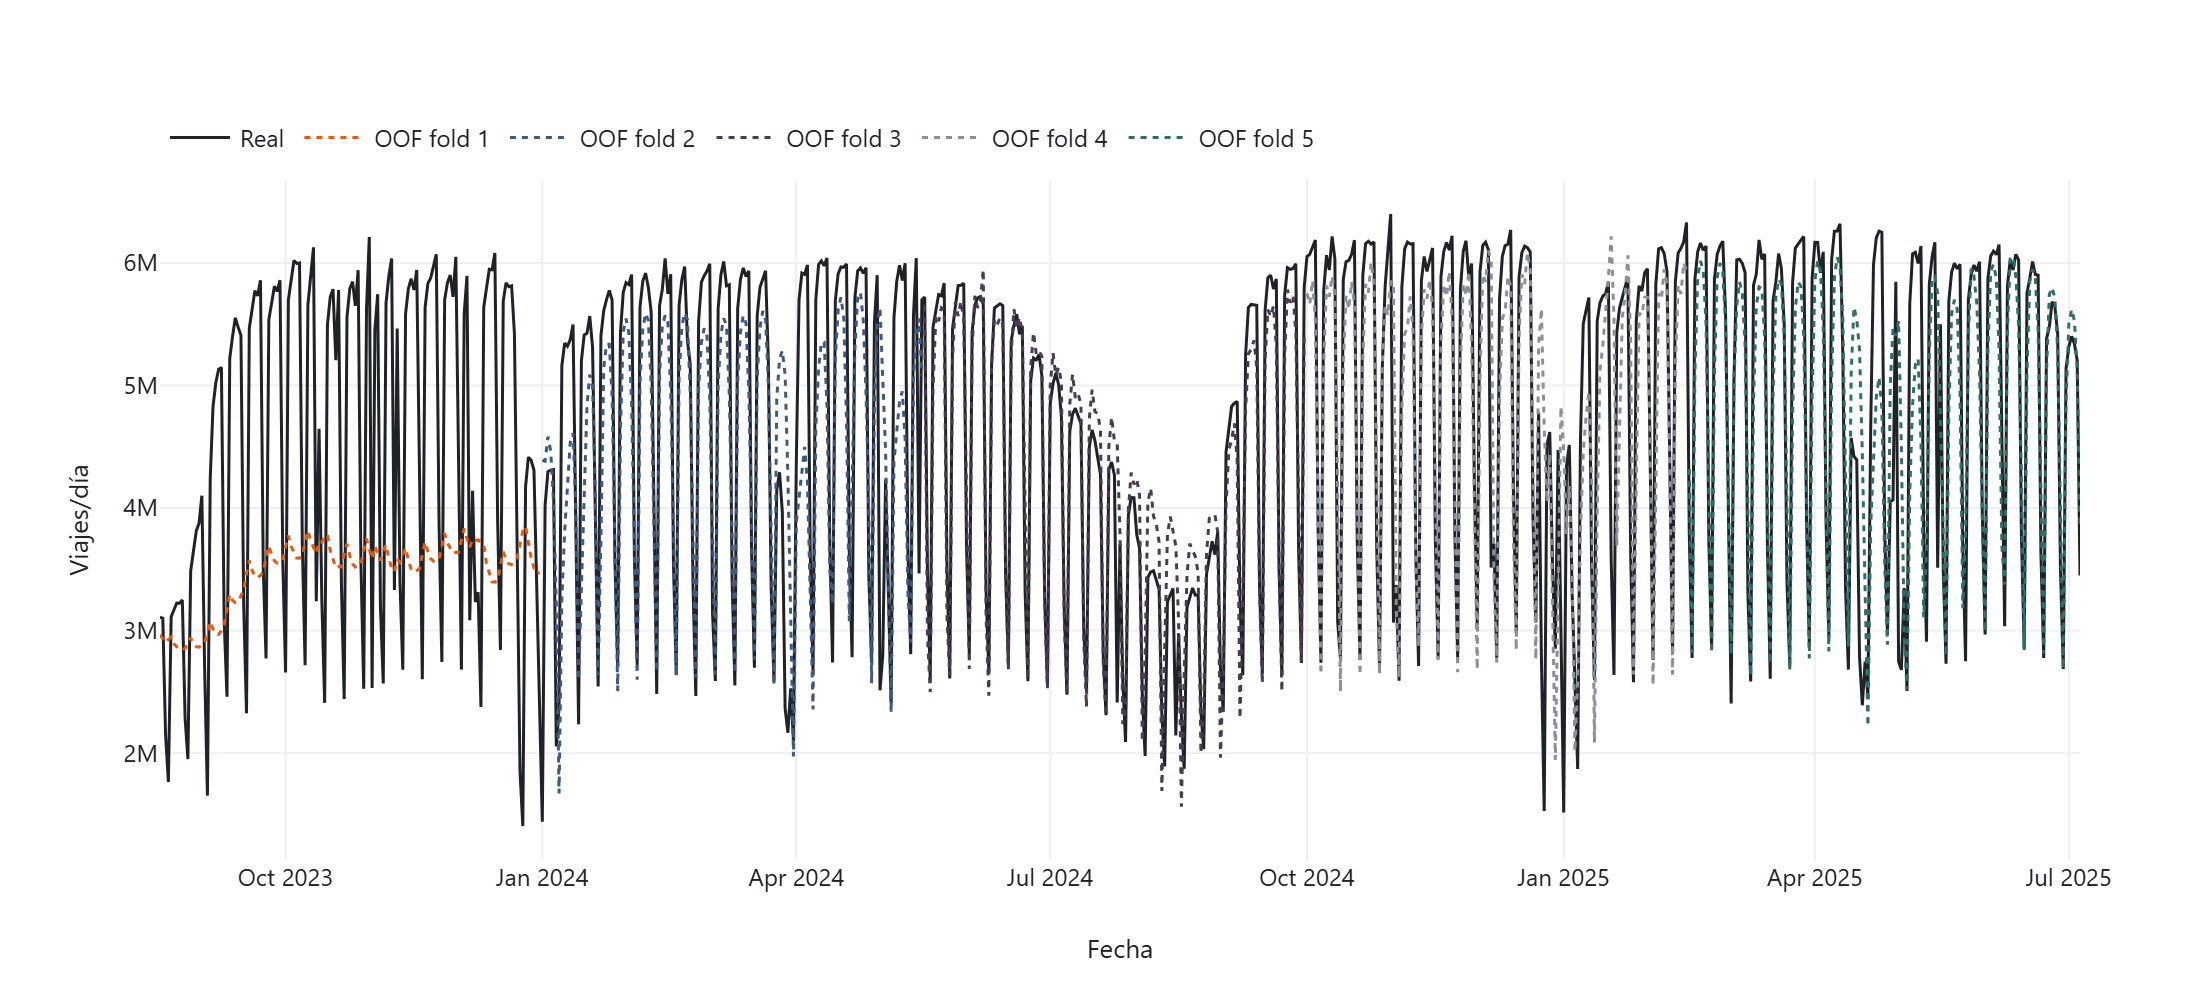
\includegraphics[width=0.78\textwidth]{fig_oof_folds.png}
  \caption{\headlinecolor{Predicción LSTM fuera de muestra (OOF) por fold del \emph{walk-forward} expansivo.}}
  \label{fig:oof_folds}
\end{figure}

Las 200 primeras filas de entrenamiento (2023-01-29 a 2023-08-16) no reciben ninguna
predicción OOF, puesto que evaluarlas exigiría un modelo entrenado con menos observaciones
que la ventana mínima inicial que el esquema considera aceptable; estas filas se
conservan en el fichero de salida marcadas explícitamente como \texttt{has\_oof=False},
con su motivo de exclusión indicado, en lugar de eliminarse sin más. La cobertura efectiva
resultante es de 689 de las 889 filas de entrenamiento (77,5\,\%), con un MAE OOF agregado
de 690.460 y un RMSE de 997.520.

El fold 1 merece un análisis detallado porque su comportamiento es \textbf{degenerado} y
la decisión que se toma sobre él condiciona directamente el conjunto de entrenamiento de
la etapa 2. Entrenado sobre apenas 200 observaciones (172 secuencias, reducidas a 147 tras
separar la cola de parada anticipada), sus predicciones fuera de muestra presentan una
desviación típica de solo el 0,199 de la de los valores reales y una correlación de
apenas 0,300 con ellos: el modelo, con tan poco historial disponible, nunca llega a
escapar de predecir un valor próximo a una constante, y la parada anticipada se activa ya
en la época 15 sobre una señal de validación interna construida con solo 25 secuencias,
demasiado ruidosa para guiar el entrenamiento de forma fiable. La figura
\ref{fig:oof_fold1_degenerado} contrasta visualmente esta degeneración con el fold 3, sano
por comparación (correlaciones entre 0,79 y 0,95 en los folds 2 a 5, frente al 0,300 del
fold 1).

\begin{figure}[htbp]
  \centering
  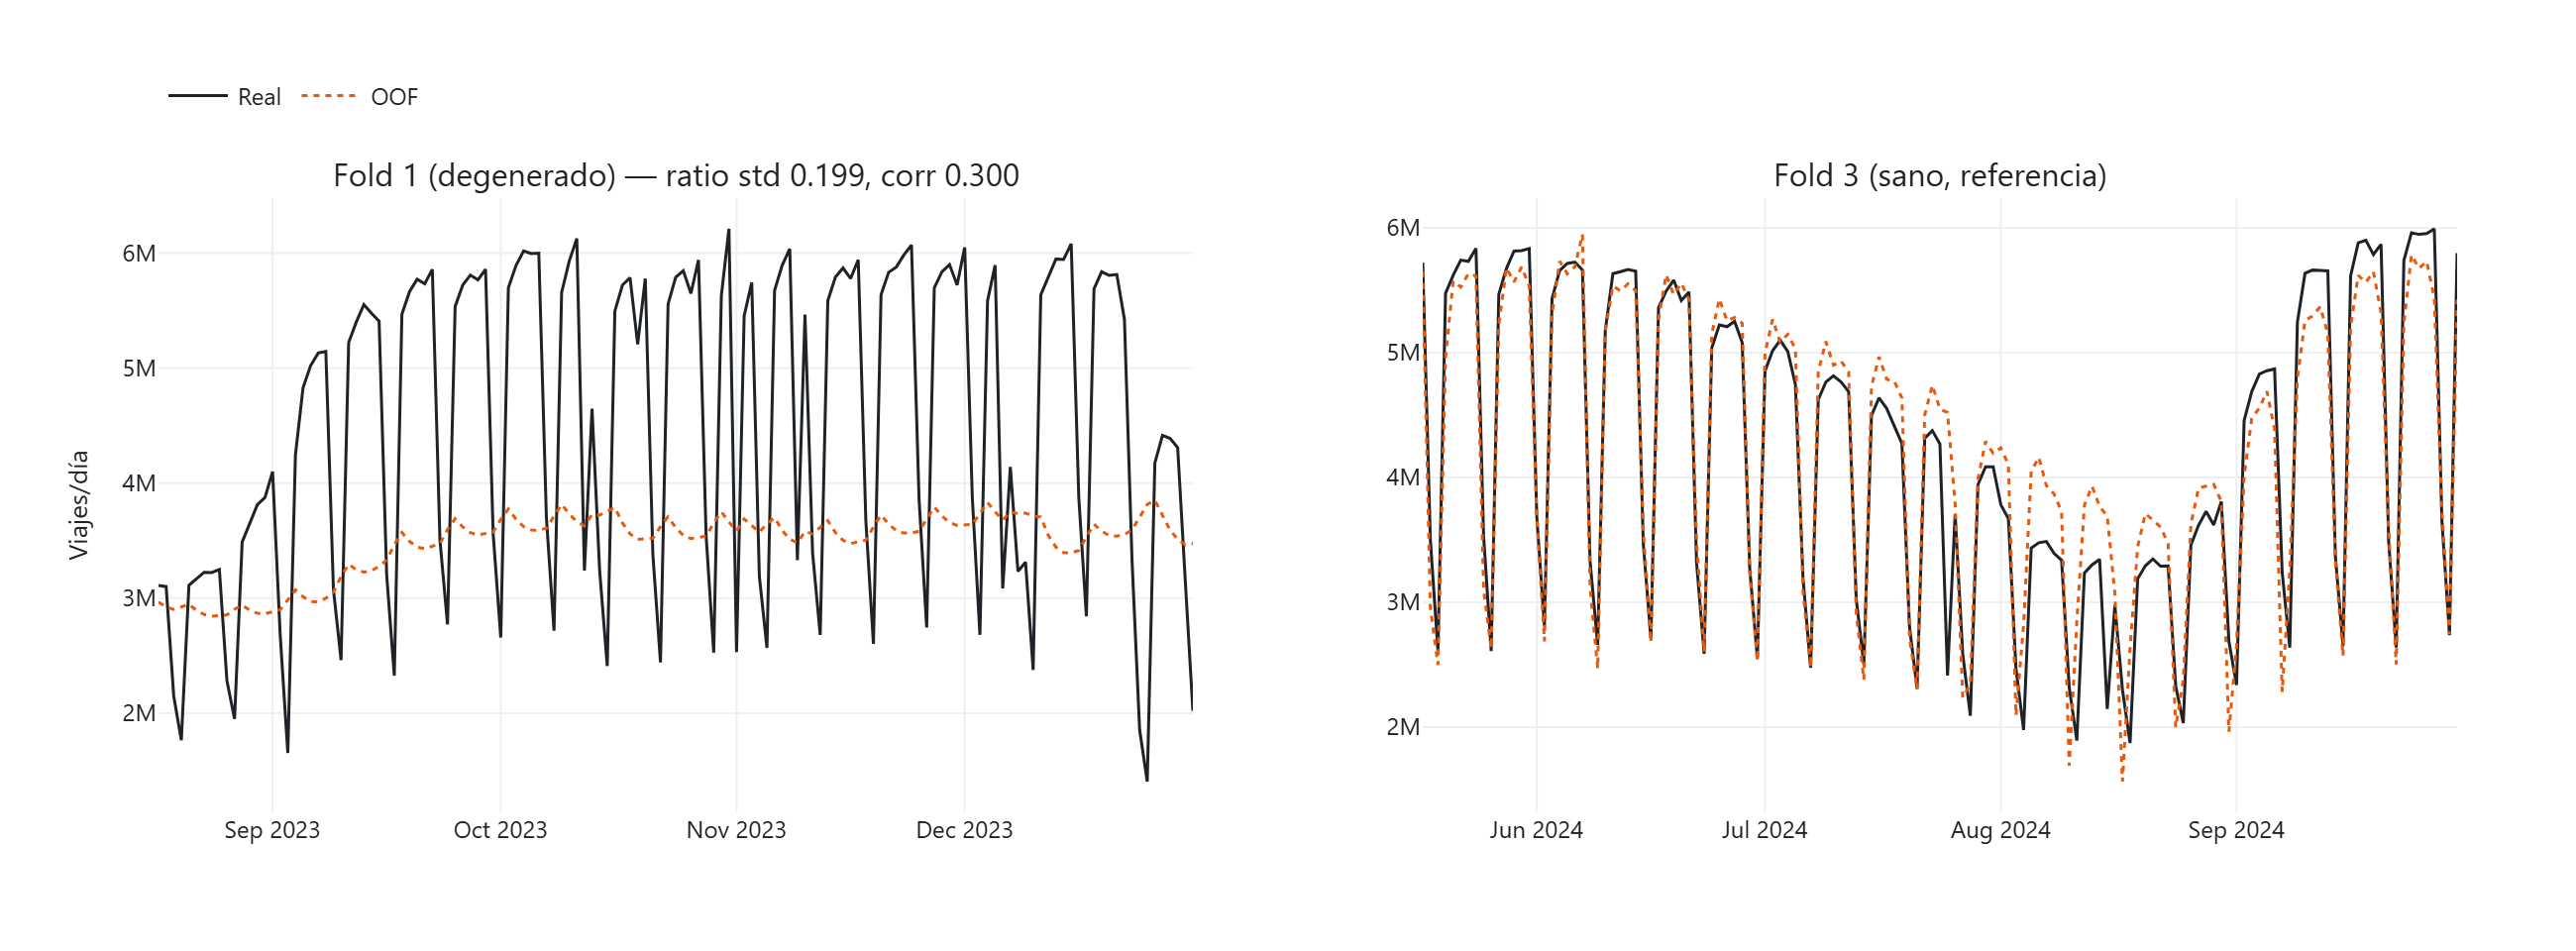
\includegraphics[width=0.78\textwidth,keepaspectratio]{fig_oof_fold1_degenerado.png}
  \caption{\headlinecolor{Fold 1 del esquema OOF es degenerado (predicción casi constante) frente al fold 3 (sano, referencia).}}
  \label{fig:oof_fold1_degenerado}
\end{figure}

La consecuencia práctica es que las 137 filas del fold 1 se \textbf{excluyen} del
conjunto de entrenamiento de la etapa 2 (\ref{sec:etapa2_xgboost}): sus residuos están
dominados por el fallo estructural de un modelo con historial insuficiente, no por la
estructura de calendario que se pretende que XGBoost aprenda, e incorporarlos
introduciría ruido de una naturaleza distinta a la del resto del conjunto residual. Esta
exclusión no se decide por intuición, sino que se somete a una comprobación explícita de
cobertura de categorías: para cada nivel categórico presente en el fold 1 (tipo de día,
tipo de festividad, indicador de día puente) se verifica que ese mismo nivel reaparece con
observaciones suficientes en los folds 2 a 5 restantes. Ninguna categoría queda huérfana
tras la exclusión, de modo que eliminar el fold 1 retira redundancia de cobertura y no
información única e insustituible; de haberse detectado una categoría con cobertura
exclusiva en el fold 1, el procedimiento habría detenido la exclusión en lugar de
proceder de todos modos.

\section{Etapa 2: XGBoost sobre el residuo}\label{sec:etapa2_xgboost}

Tras retirar las 200 filas sin predicción OOF y las 137 filas del fold 1 degenerado, el
conjunto de entrenamiento de la etapa 2 queda formado por 552 filas, desde el
2024-01-01 hasta el 2025-07-05, con las 161 variables predictoras de la sección
\ref{sec:ingenieria_features} y sin ningún valor nulo. La variable objetivo de esta etapa
no es la demanda sino el residuo definido en la introducción del capítulo,
$e_t = y_t - \hat y^{\text{LSTM}}_t$, calculado exclusivamente a partir de las
predicciones fuera de muestra de la sección anterior; su signo se fija de modo que la
corrección de la etapa 2 se \emph{suma} a la predicción de la etapa 1. El residuo
presenta una media de 109.601 y una desviación típica de 726.669 sobre un rango de
$[-3.128.729,\ +1.899.895]$: una dispersión del mismo orden de magnitud que la propia
señal de demanda, lo que anticipa que corregirlo es, en sí mismo, un problema de
predicción exigente.

XGBoost \parencite{chen2016xgboost} se entrena sobre este conjunto residual con los
hiperparámetros de la tabla \ref{tab:hiperparametros}, seleccionados mediante una rejilla
de 54 combinaciones evaluada sobre un \emph{holdout} interno cronológico (el último
15\,\% de las fechas del propio conjunto de entrenamiento del modelo, nunca la partición
de validación oficial) y reajustados después sobre la totalidad de los datos disponibles
para ese modelo. La configuración ganadora combina árboles relativamente profundos
($\text{max\_depth}=5$) con una tasa de aprendizaje baja (0,01) y un número elevado de
estimadores (300), junto con una regularización moderada por tamaño mínimo de nodo
($\text{min\_child\_weight}=3$); esta combinación resulta coherente con un conjunto de
entrenamiento reducido (552 filas) y una señal de calendario dispersa y de bajo peso
relativo frente al ruido introducido por la propia etapa 1.

\begin{table}[htbp]
  \centering
  \small
  \setlength{\tabcolsep}{4pt}
  \resizebox{\textwidth}{!}{%
    \begin{tabular}{>{\raggedright\arraybackslash}p{3.0cm}>{\centering\arraybackslash}p{2.3cm}>{\centering\arraybackslash}p{1.8cm}>{\centering\arraybackslash}p{2.1cm}>{\centering\arraybackslash}p{2.0cm}>{\centering\arraybackslash}p{2.3cm}}
\toprule
\rowcolor{naranja}
\textbf{Modelo} & \textbf{Filas entrenamiento} & \textbf{max\_\allowbreak{}depth} & \textbf{n\_\allowbreak{}estimators} & \textbf{learning\_\allowbreak{}rate} & \textbf{min\_\allowbreak{}child\_\allowbreak{}weight} \\
\midrule
\rowcolor{filaclara} xgboost\_\allowbreak{}residual & 552 & 5 & 300 & 0,01 & 3 \\
xgboost\_\allowbreak{}alone & 889 & 5 & 100 & 0,05 & 10 \\
\bottomrule
\end{tabular}
%
  }
  \caption{\headlinecolor{Hiperparámetros seleccionados por búsqueda en rejilla de 54 puntos (idéntico para ambos modelos XGBoost) sobre un \emph{holdout} interno cronológico.}}
  \label{tab:hiperparametros}
\end{table}

La variable individual con mayor ganancia en este modelo es
\texttt{feat\_\allowbreak{}day\_\allowbreak{}type\_\allowbreak{}festivo} (ganancia 0,125;
tabla \ref{tab:top15_residual}, capítulo \ref{cap:resultados}), lo que apunta a
que la etapa 2 sí aprende, a partir de las variables exógenas, la señal de calendario que
la etapa 1 no puede ver por diseño: el mecanismo que motiva la arquitectura híbrida se
observa de forma medible, con independencia de que el resultado agregado del
capítulo \ref{cap:resultados} termine siendo, o no, favorable a la arquitectura completa.

Conviene dejar constancia, en este punto y no como un descubrimiento tardío en la
discusión de resultados, de una limitación estructural del esquema de \emph{stacking}
OOF empleado. Los cinco modelos LSTM que generan los residuos de entrenamiento se ajustan,
según el fold, sobre entre 337 y 748 filas, mientras que el modelo LSTM final que se
emplea en inferencia, el descrito en la sección \ref{sec:etapa1_lstm}, se entrena sobre
las 889 filas completas y es, previsiblemente, algo mejor que cualquiera de los modelos
parciales que generaron los residuos de entrenamiento. En consecuencia, la etapa 2 aprende
a corregir una distribución de residuo ligeramente más ancha que la que el sistema
realmente enfrenta en inferencia. Este desajuste es inherente a cualquier esquema de
\emph{stacking} fuera de muestra —la alternativa, usar residuos \emph{in-sample} del
modelo final, es estrictamente peor por las razones expuestas en la sección
\ref{sec:esquema_oof}— y se acepta aquí como el coste asumido de evitar una fuga de
información mucho más grave.

\section{Modelos de control}\label{sec:modelos_control}

Para poder atribuir el desempeño del híbrido a su arquitectura, y no simplemente al hecho
de disponer de variables exógenas, es necesario compararlo contra un control que utilice
exactamente las mismas 161 variables sin pasar por ninguna etapa LSTM previa. Este control,
denominado \texttt{xgboost\_alone}, entrena un modelo XGBoost directamente sobre la
demanda total, con idéntico procedimiento de ajuste de hiperparámetros que el modelo
residual de la sección anterior y sobre la misma matriz de características. Su función es
aislar si la etapa 1 aporta valor incremental a la predicción final o si, por el
contrario, introduce ruido que un modelo de una sola etapa evitaría directamente.

Una decisión que podría parecer, a primera vista, una inconsistencia entre ambos modelos
es deliberada: \texttt{xgboost\_alone} se entrena sobre las 889 filas completas del
conjunto de entrenamiento posterior al calentamiento, no sobre las 552 filas del conjunto
residual de la etapa 2. La razón es que \texttt{xgboost\_alone} no depende en ningún
momento de las predicciones OOF de la etapa 1, de modo que ni la exclusión de las 200
filas sin cobertura OOF ni la exclusión del fold 1 degenerado le son aplicables:
imponérselas de todos modos, en nombre de una supuesta igualdad de condiciones, habría
privado al control de un tercio de su historial de entrenamiento disponible por una razón
que le es completamente ajena. La matriz de variables y el procedimiento de ajuste de
hiperparámetros son, por tanto, idénticos entre ambos modelos XGBoost; el tamaño del
conjunto de entrenamiento, legítimamente, no lo es.

La propuesta inicial de este TFM contemplaba, junto a XGBoost, un segundo representante
de la familia de aprendizaje automático tabular (bosques aleatorios, \emph{random forest}). Se ha prescindido
de él de forma deliberada: ambos son métodos de conjunto sobre árboles de decisión y
comparten la misma capacidad de representación sobre esta matriz de características, de
modo que un segundo representante habría añadido una fila más a la comparación maestra
sin poner a prueba ninguna hipótesis distinta. El esfuerzo de control se ha destinado, en
su lugar, a los experimentos de \emph{paridad informativa} de la sección
\ref{sec:paridad_informativa} (ablación de bloques de variables y LSTM con acceso a la
matriz predictora completa), diseñados para discriminar entre las explicaciones rivales del
resultado central de este trabajo.

Como complemento a este control directo, la sección \ref{sec:analisis_sensibilidad} del
capítulo \ref{cap:resultados} introduce una variante adicional de la etapa 2,
\texttt{hybrid\_weighted}, que no constituye un modelo nuevo, sino una reponderación del
mismo modelo residual: idéntica en las 552 filas de entrenamiento, las 161 variables, la
semilla aleatoria y los hiperparámetros (cargados directamente del modelo de la sección
\ref{sec:etapa2_xgboost} en lugar de reajustarse de forma independiente, precisamente
para que ambas variantes sean comparables sin introducir una segunda fuente de
variación), y que difiere únicamente en que asigna un peso de muestra triple a las filas
correspondientes a días de calendario irregular (festivos y días puente), un 8,2\,\% del
conjunto residual. El objetivo de esta variante es comprobar si concentrar la capacidad
del modelo en los días donde la etapa 1 falla con mayor intensidad (festivos y puentes,
según el diagnóstico de la sección \ref{sec:diagnostico_previo}) mejora la corrección precisamente en
esos días; su evaluación completa, con un criterio de éxito fijado antes de observar el
resultado, se desarrolla en la sección \ref{sec:experimento_a} y no se anticipa aquí.

\section{Ensamble por combinación de pronósticos}\label{sec:metodologia_ensemble}

SARIMAX (sección \ref{sec:baselines}) y el control \texttt{xgboost\_alone} de la sección anterior
no solo se emplean por separado como adversarios del híbrido: sus predicciones, ya
generadas y persistidas, permiten formular sin ningún coste de entrenamiento adicional
un tercer candidato —una combinación lineal de ambos— cuya justificación conviene
formalizar aquí, como parte del diseño experimental, y no introducir por primera vez
al presentar sus resultados en el capítulo \ref{cap:resultados}. Dados los pronósticos
puntuales de ambos modelos en el instante $t$, $\hat y_t^{\text{SARIMAX}}$ y
$\hat y_t^{\text{XGB}}$, el ensamble se define como la combinación lineal convexa
\[
  \hat y_t = w_1\, \hat y_t^{\text{SARIMAX}} + w_2\, \hat y_t^{\text{XGB}},
  \qquad w_1 + w_2 = 1,\ w_1, w_2 \geq 0,
\]
una operación puramente aritmética sobre predicciones ya calculadas, sin reentrenar
ningún modelo ni introducir ningún parámetro adicional que deba ajustarse por
descenso de gradiente.

La justificación de que una combinación tan simple pueda superar a ambos componentes
individuales no es heurística: descansa en la identidad de reducción de varianza de Bates y
Granger y en la condición de Granger sobre conjuntos de información distintos, ambas
expuestas en la sección \ref{sec:arquitecturas_hibridas}. Lo que importa fijar aquí es que
SARIMAX y \texttt{xgboost\_alone} \emph{sí} satisfacen esa condición: sus conjuntos de
información se solapan pero no se anidan. El primero condiciona sobre el historial completo
de la serie mediante su componente $(p,d,q)\times(P,D,Q,s)$ con diferenciación estacional
y solo cinco indicadores de calendario; el segundo dispone de una memoria de la serie
limitada a siete retardos y cuatro estadísticos móviles, pero añade los retardos de
operador, los armónicos de Fourier, la codificación completa de calendario y la
meteorología retardada, sin estructura autorregresiva ni diferenciación. El híbrido
secuencial de este TFM, en cambio, no la satisface plenamente, porque el pasado reciente que ve su
etapa 1 está representado en la matriz de su etapa 2 (sección
\ref{sec:resultado_negativo_teoria}).

Se contemplan, por diseño y antes de observar ningún resultado, dos estrategias de
ponderación. La primera, \texttt{ensemble\_equal}, fija $w_1 = w_2 = 0{,}5$: no requiere
ningún dato adicional para determinarse y actúa como el punto de referencia neutro de
la combinación. La segunda, \texttt{ensemble\_inverse\_mae}, pondera cada componente en
proporción inversa a su MAE sobre la partición de validación, de modo que el modelo
históricamente más preciso recibe mayor peso; sus coeficientes se derivan
exclusivamente de la validación y nunca de la partición de test, preservando la
separación estricta entre selección de configuración y evaluación final que gobierna
todo este TFM. Ambas variantes se evalúan en el capítulo \ref{cap:resultados}
(secciones \ref{sec:analisis_sensibilidad} y \ref{sec:mecanismo_ensemble}), donde se
cuantifica empíricamente la correlación de error $\rho$ entre SARIMAX y
\texttt{xgboost\_alone} y se pone la ganancia observada en relación con la reducción de
varianza que la identidad de Bates y Granger anticipa; se adelanta únicamente que ese contraste
sitúa a \texttt{ensemble\_equal} y \texttt{ensemble\_inverse\_mae} como los dos modelos
más precisos de todo el estudio (MAE de test 139.725 y 139.681, respectivamente),
prácticamente indistinguibles entre sí, lo que hace preferible la variante
equiponderada por no depender de ningún dato de validación para fijar sus pesos.

\chapter{Evaluación experimental del sistema predictivo}\label{cap:resultados}

Este capítulo es el núcleo empírico del TFM: presenta y discute los resultados de los
once modelos descritos o derivados en el capítulo \ref{cap:metodologia}, evaluados sobre
las particiones de validación y test definidas en la sección \ref{sec:particiones_fuga}.
Ninguna cifra se introduce manualmente: todas llegan al documento desde los artefactos
persistidos por las fases 3 a 5b, por la cadena que detalla el Anexo \ref{cap:anexo3}.
La respuesta al contraste central del TFM (\ref{sec:contraste_central}) se
somete a tres controles diagnósticos independientes: la anatomía del residuo de la etapa 1
(\ref{sec:anatomia_residuo_etapa1}), la paridad informativa entre etapas
(\ref{sec:paridad_informativa}) y el desglose por subgrupos y periodos con corrección por
comparaciones múltiples (\ref{sec:desglose_subgrupos}).

\section{Tabla maestra de comparación}\label{sec:tabla_maestra}

Las tablas \ref{tab:comparacion_test} y \ref{tab:comparacion_val} reúnen los once modelos
de este TFM (cuatro baselines ingenuos, dos modelos de una sola etapa, tres variantes de
la familia LSTM y dos variantes de ensamble) ordenados de mejor a peor por MAE sobre las
particiones de test y de validación respectivamente. El coeficiente de determinación se
reporta a cuatro decimales y no a dos, una asimetría deliberada frente al resto de
métricas: a dos decimales, \texttt{ensemble\_equal} (0,9755), \texttt{xgboost\_alone}
(0,9690) y \texttt{sarimax} (0,9672) colapsarían en 0,98/0,97/0,97, borrando exactamente
la distinción que esta comparación existe para establecer. El MAPE, en cambio, no sufre
ese problema a esta escala y se mantiene a dos decimales.

\begin{table}[htbp]
  \centering
  \small
  \setlength{\tabcolsep}{4pt}
  \resizebox{\textwidth}{!}{\begin{tabular}{>{\raggedright\arraybackslash}p{3.2cm}>{\raggedright\arraybackslash}p{2.4cm}>{\centering\arraybackslash}p{0.8cm}>{\centering\arraybackslash}p{1.7cm}>{\centering\arraybackslash}p{1.7cm}>{\centering\arraybackslash}p{1.7cm}>{\centering\arraybackslash}p{1.4cm}}
\toprule
\rowcolor{naranja}
\textbf{Modelo} & \textbf{Familia} & \textbf{n} & \textbf{MAE} & \textbf{RMSE} & \textbf{MAPE (\%)} & \textbf{R²} \\
\midrule
\rowcolor{filaclara} ensemble\_\allowbreak{}inverse\_\allowbreak{}mae & Ensemble & 197 & 139.681 & 208.339 & 3,11 & 0,9755 \\
ensemble\_\allowbreak{}equal & Ensemble & 197 & 139.725 & 208.464 & 3,13 & 0,9755 \\
\rowcolor{filaclara} xgboost\_\allowbreak{}alone & Una etapa & 197 & 156.121 & 234.154 & 3,30 & 0,9690 \\
sarimax & Una etapa & 197 & 163.627 & 241.147 & 3,85 & 0,9672 \\
\rowcolor{filaclara} hybrid\_\allowbreak{}weighted & Familia LSTM & 197 & 220.286 & 319.447 & 5,17 & 0,9424 \\
hybrid & Familia LSTM & 197 & 234.223 & 328.131 & 5,49 & 0,9392 \\
\rowcolor{filaclara} lstm\_\allowbreak{}alone & Familia LSTM & 197 & 280.952 & 431.714 & 6,62 & 0,8948 \\
seasonal\_\allowbreak{}naive & Baseline ingenuo & 197 & 309.817 & 690.480 & 7,16 & 0,7308 \\
\rowcolor{filaclara} persistence & Baseline ingenuo & 197 & 900.570 & 1.390.444 & 21,79 & -0,0916 \\
moving\_\allowbreak{}average\_\allowbreak{}7 & Baseline ingenuo & 197 & 1.093.679 & 1.260.492 & 28,13 & 0,1029 \\
\rowcolor{filaclara} moving\_\allowbreak{}average\_\allowbreak{}28 & Baseline ingenuo & 197 & 1.119.987 & 1.301.939 & 28,74 & 0,0430 \\
\bottomrule
\end{tabular}
}
  \caption{\headlinecolor{Comparación de modelos, partición TEST (n=197, 2026-01-18 a 2026-08-02).}}
  \label{tab:comparacion_test}
\end{table}

\begin{table}[htbp]
  \centering
  \small
  \setlength{\tabcolsep}{4pt}
  \resizebox{\textwidth}{!}{\begin{tabular}{>{\raggedright\arraybackslash}p{3.2cm}>{\raggedright\arraybackslash}p{2.4cm}>{\centering\arraybackslash}p{0.8cm}>{\centering\arraybackslash}p{1.7cm}>{\centering\arraybackslash}p{1.7cm}>{\centering\arraybackslash}p{1.7cm}>{\centering\arraybackslash}p{1.4cm}}
\toprule
\rowcolor{naranja}
\textbf{Modelo} & \textbf{Familia} & \textbf{n} & \textbf{MAE} & \textbf{RMSE} & \textbf{MAPE (\%)} & \textbf{R²} \\
\midrule
\rowcolor{filaclara} ensemble\_\allowbreak{}inverse\_\allowbreak{}mae & Ensemble & 196 & 226.418 & 323.348 & 5,62 & 0,9519 \\
ensemble\_\allowbreak{}equal & Ensemble & 196 & 227.588 & 324.752 & 5,69 & 0,9515 \\
\rowcolor{filaclara} xgboost\_\allowbreak{}alone & Una etapa & 196 & 244.843 & 355.027 & 5,68 & 0,9420 \\
sarimax & Una etapa & 196 & 273.467 & 404.153 & 7,31 & 0,9248 \\
\rowcolor{filaclara} hybrid\_\allowbreak{}weighted & Familia LSTM & 196 & 276.347 & 401.456 & 6,94 & 0,9258 \\
hybrid & Familia LSTM & 196 & 280.738 & 415.562 & 7,09 & 0,9205 \\
\rowcolor{filaclara} lstm\_\allowbreak{}alone & Familia LSTM & 196 & 411.142 & 655.479 & 11,81 & 0,8023 \\
seasonal\_\allowbreak{}naive & Baseline ingenuo & 196 & 460.615 & 883.627 & 12,63 & 0,6408 \\
\rowcolor{filaclara} persistence & Baseline ingenuo & 196 & 914.119 & 1.387.393 & 23,72 & 0,1144 \\
moving\_\allowbreak{}average\_\allowbreak{}7 & Baseline ingenuo & 196 & 1.068.961 & 1.237.156 & 28,86 & 0,2958 \\
\rowcolor{filaclara} moving\_\allowbreak{}average\_\allowbreak{}28 & Baseline ingenuo & 196 & 1.137.759 & 1.357.281 & 31,12 & 0,1524 \\
\bottomrule
\end{tabular}
}
  \caption{\headlinecolor{Comparación de modelos, partición VAL (n=196, 2025-07-06 a 2026-01-17).}}
  \label{tab:comparacion_val}
\end{table}

La jerarquía resultante es nítida y consistente entre ambas particiones, como confirma
la figura \ref{fig:model_comparison_bar_test}.
En primer lugar, las dos variantes de ensamble (combinaciones puramente aritméticas de
SARIMAX y \texttt{xgboost\_alone}, sin entrenamiento adicional) lideran ambas
particiones: \texttt{ensemble\_inverse\_mae} obtiene el mejor MAE de test, \textbf{139.681}, con un
$R^2$ de 0,9755, seguido a menos de un 0,05\,\% de distancia por \texttt{ensemble\_equal}
(139.725). En segundo lugar, los dos modelos de una sola etapa ocupan el siguiente escalón
sin solaparse con el anterior: \texttt{xgboost\_alone} (MAE test 156.121, $R^2=0{,}9690$) y
SARIMAX (MAE test 163.627, $R^2=0{,}9672$) mejoran de forma clara a toda la familia LSTM
que seguirá describiéndose en las secciones siguientes, pero quedan por detrás del
ensamble en aproximadamente un 11\,\% y un 17\,\% de MAE respectivamente. En tercer
lugar, la familia LSTM (\texttt{hybrid\_weighted}, \texttt{hybrid} y \texttt{lstm\_alone},
en ese orden) se sitúa sistemáticamente peor que ambos modelos de una sola etapa, un
resultado que se analiza en detalle en la sección \ref{sec:contraste_central}.

Por último, los cuatro baselines ingenuos colapsan frente a cualquiera de los modelos
anteriores: la persistencia estacional, el mejor de ellos, supera en torno a un 10\,\% en
MAE al peor miembro de la familia LSTM, y la persistencia simple y las dos medias móviles presentan
$R^2$ próximos a cero o directamente negativos, confirmando sobre el conjunto completo de
modelos la advertencia ya adelantada en el capítulo \ref{cap:metodologia}: superar a la
persistencia simple es un umbral trivial en esta serie, y el resultado interesante de este
capítulo se juega enteramente entre los siete modelos restantes.

\begin{figure}[htbp]
  \centering
  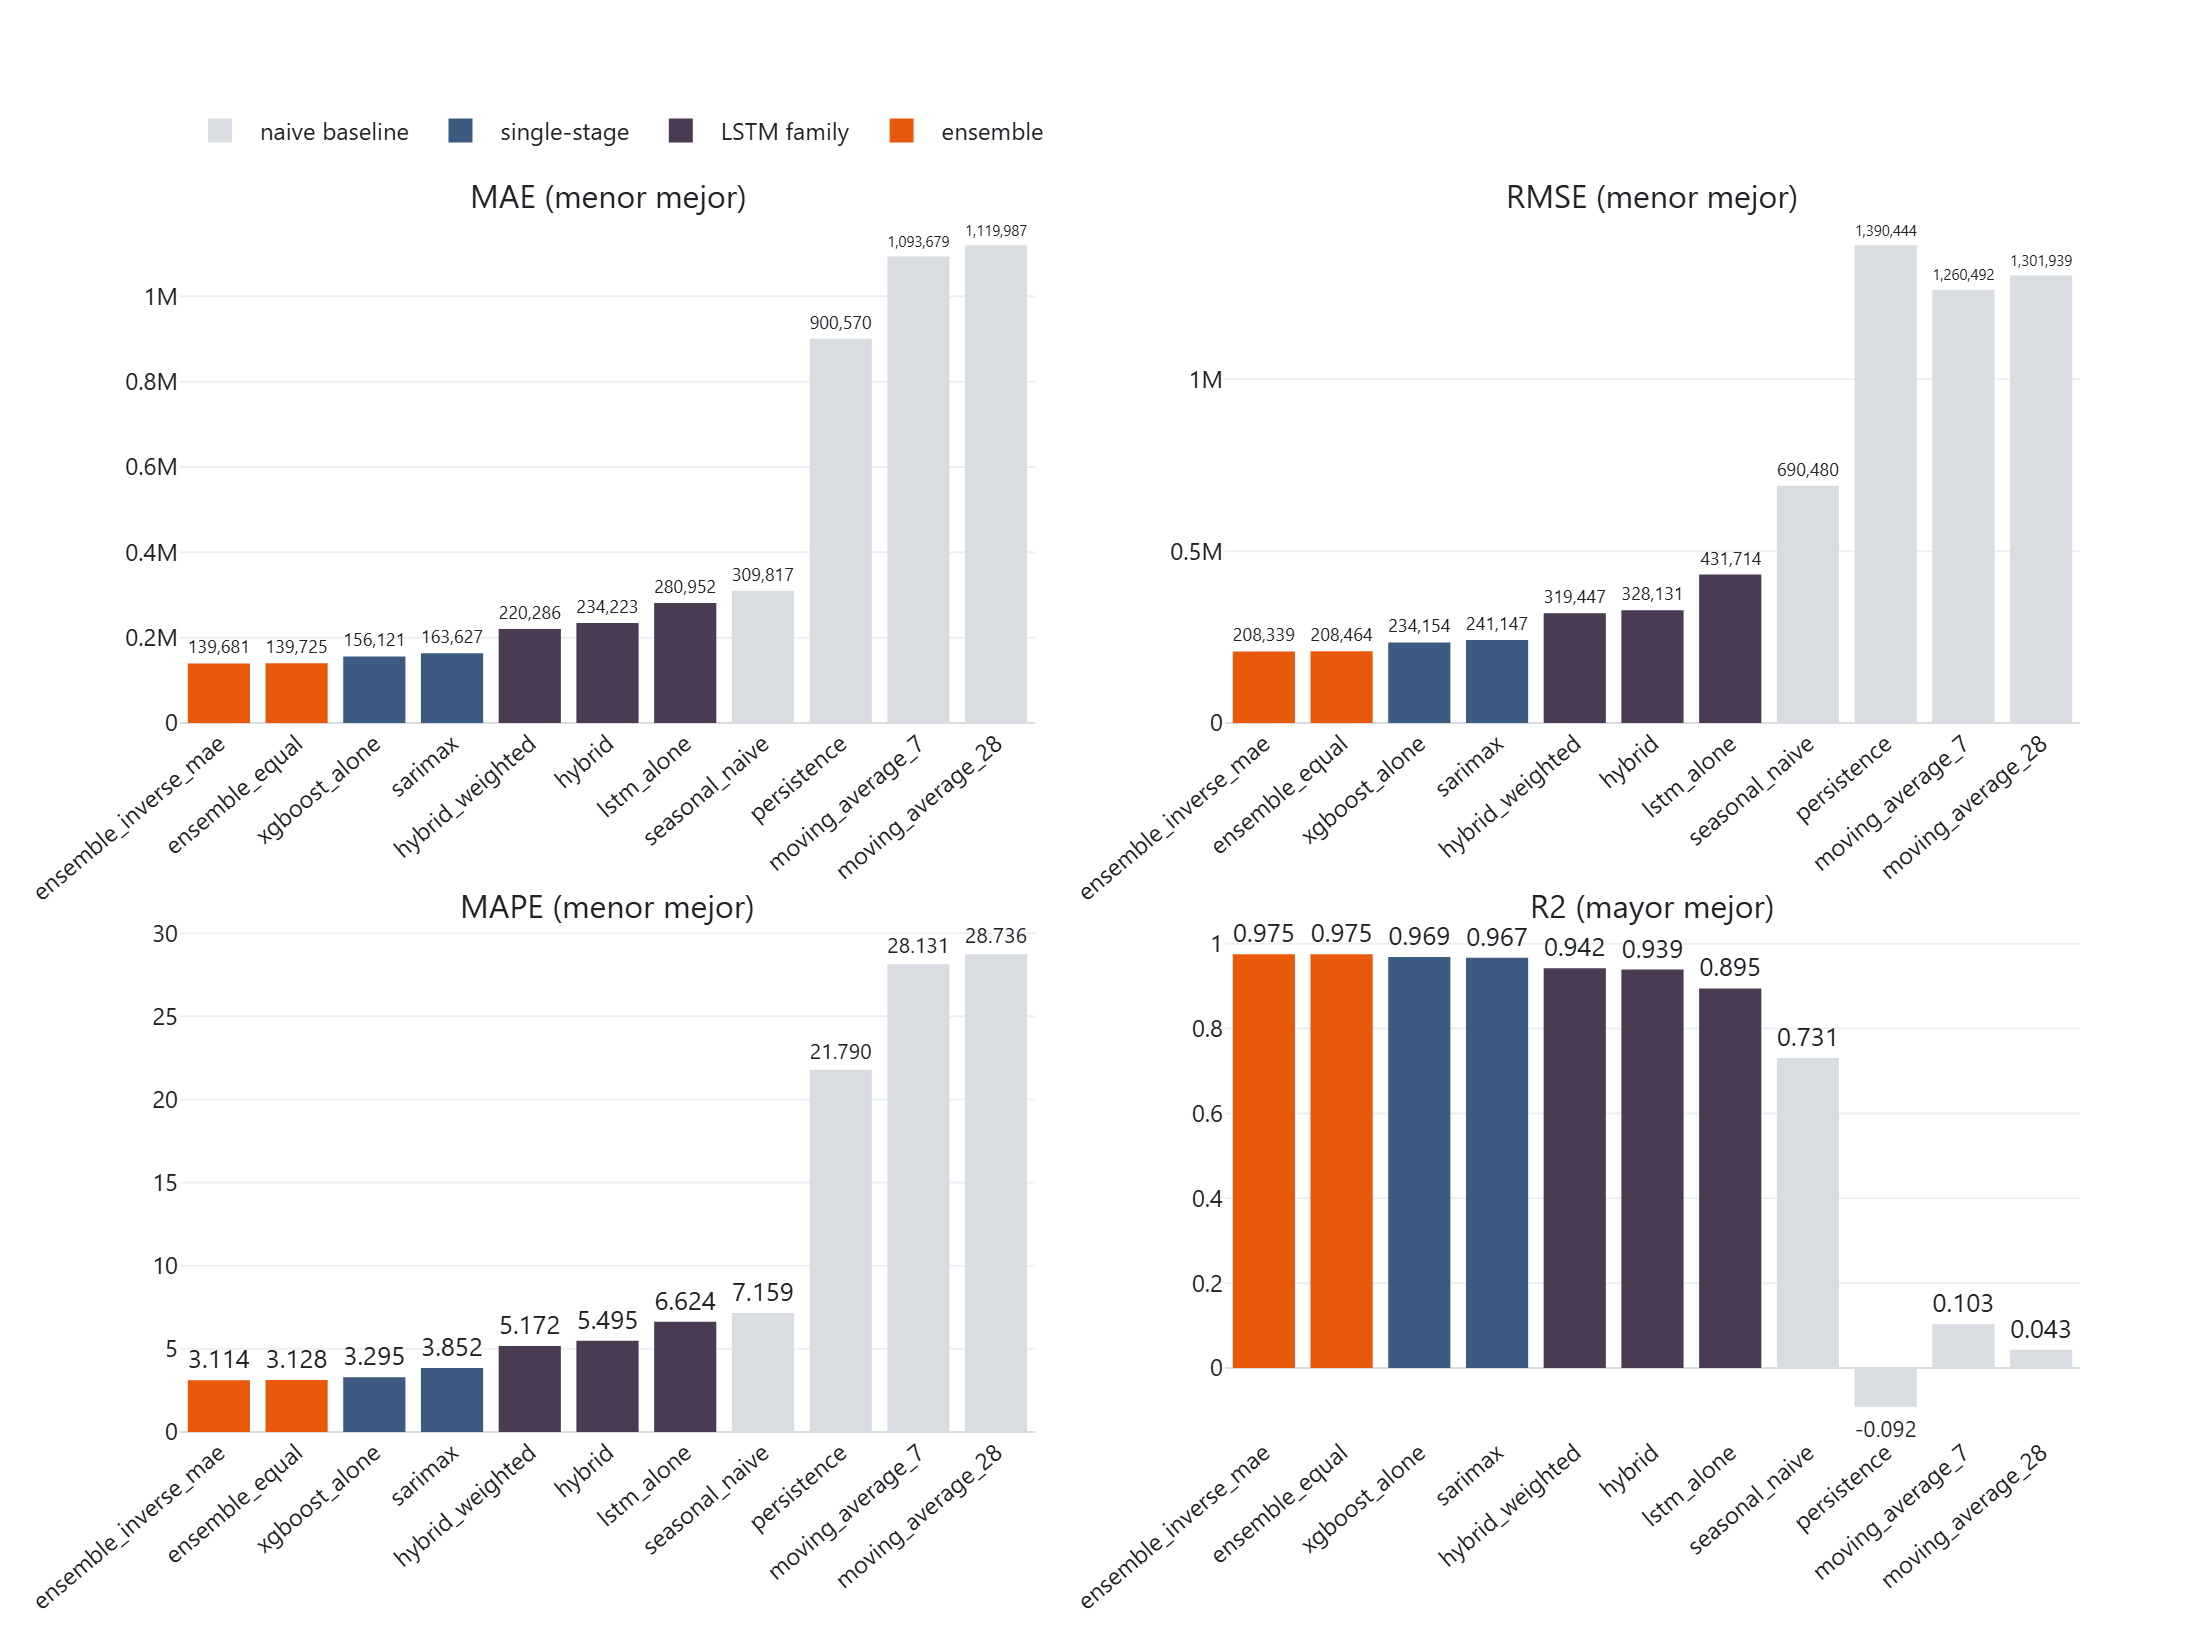
\includegraphics[width=0.78\textwidth]{model_comparison_bar_test.png}
  \caption{\headlinecolor{Comparación de modelos en la partición test. Barras agrupadas de MAE, RMSE, MAPE y $R^2$, ordenadas de mejor a peor por MAE. El color codifica la familia del modelo.}}
  \label{fig:model_comparison_bar_test}
\end{figure}

Ninguna cifra de la partición de entrenamiento se presenta junto a estas dos tablas como
si fuera una estimación válida de desempeño: train es, por construcción, una muestra
\emph{in-sample} para todo modelo que se ajusta sobre ella, y su inclusión aquí induciría
a compararla incorrectamente con val o test, un error que la sección
\ref{sec:analisis_residuos} evita explícitamente al tratar el desempeño en train como
diagnóstico de sobreajuste y no como un resultado más de la tabla maestra.

\section{Ajuste temporal}\label{sec:ajuste_temporal}

La figura \ref{fig:demand_actual_vs_predicted_test} muestra la serie real de demanda
total superpuesta a la predicción del modelo ganador, \texttt{ensemble\_equal}, sobre la
partición de test; la de validación reproduce el mismo patrón. La predicción sigue de
cerca tanto la oscilación semanal (el diente de sierra laborable/fin de semana de la
sección \ref{sec:eda}) como las transiciones asociadas a festivos aislados, sin el retraso
de fase que delataría un modelo que en realidad predijera el valor del día anterior. Las
mayores desviaciones puntuales se concentran en los días de calendario irregular, festivos
y puentes, desglosados en la sección \ref{sec:error_dia}; el resto de la serie se sigue
con una fidelidad coherente con el MAPE de test del 3,13\,\% de la tabla
\ref{tab:comparacion_test}.

\begin{figure}[htbp]
  \centering
  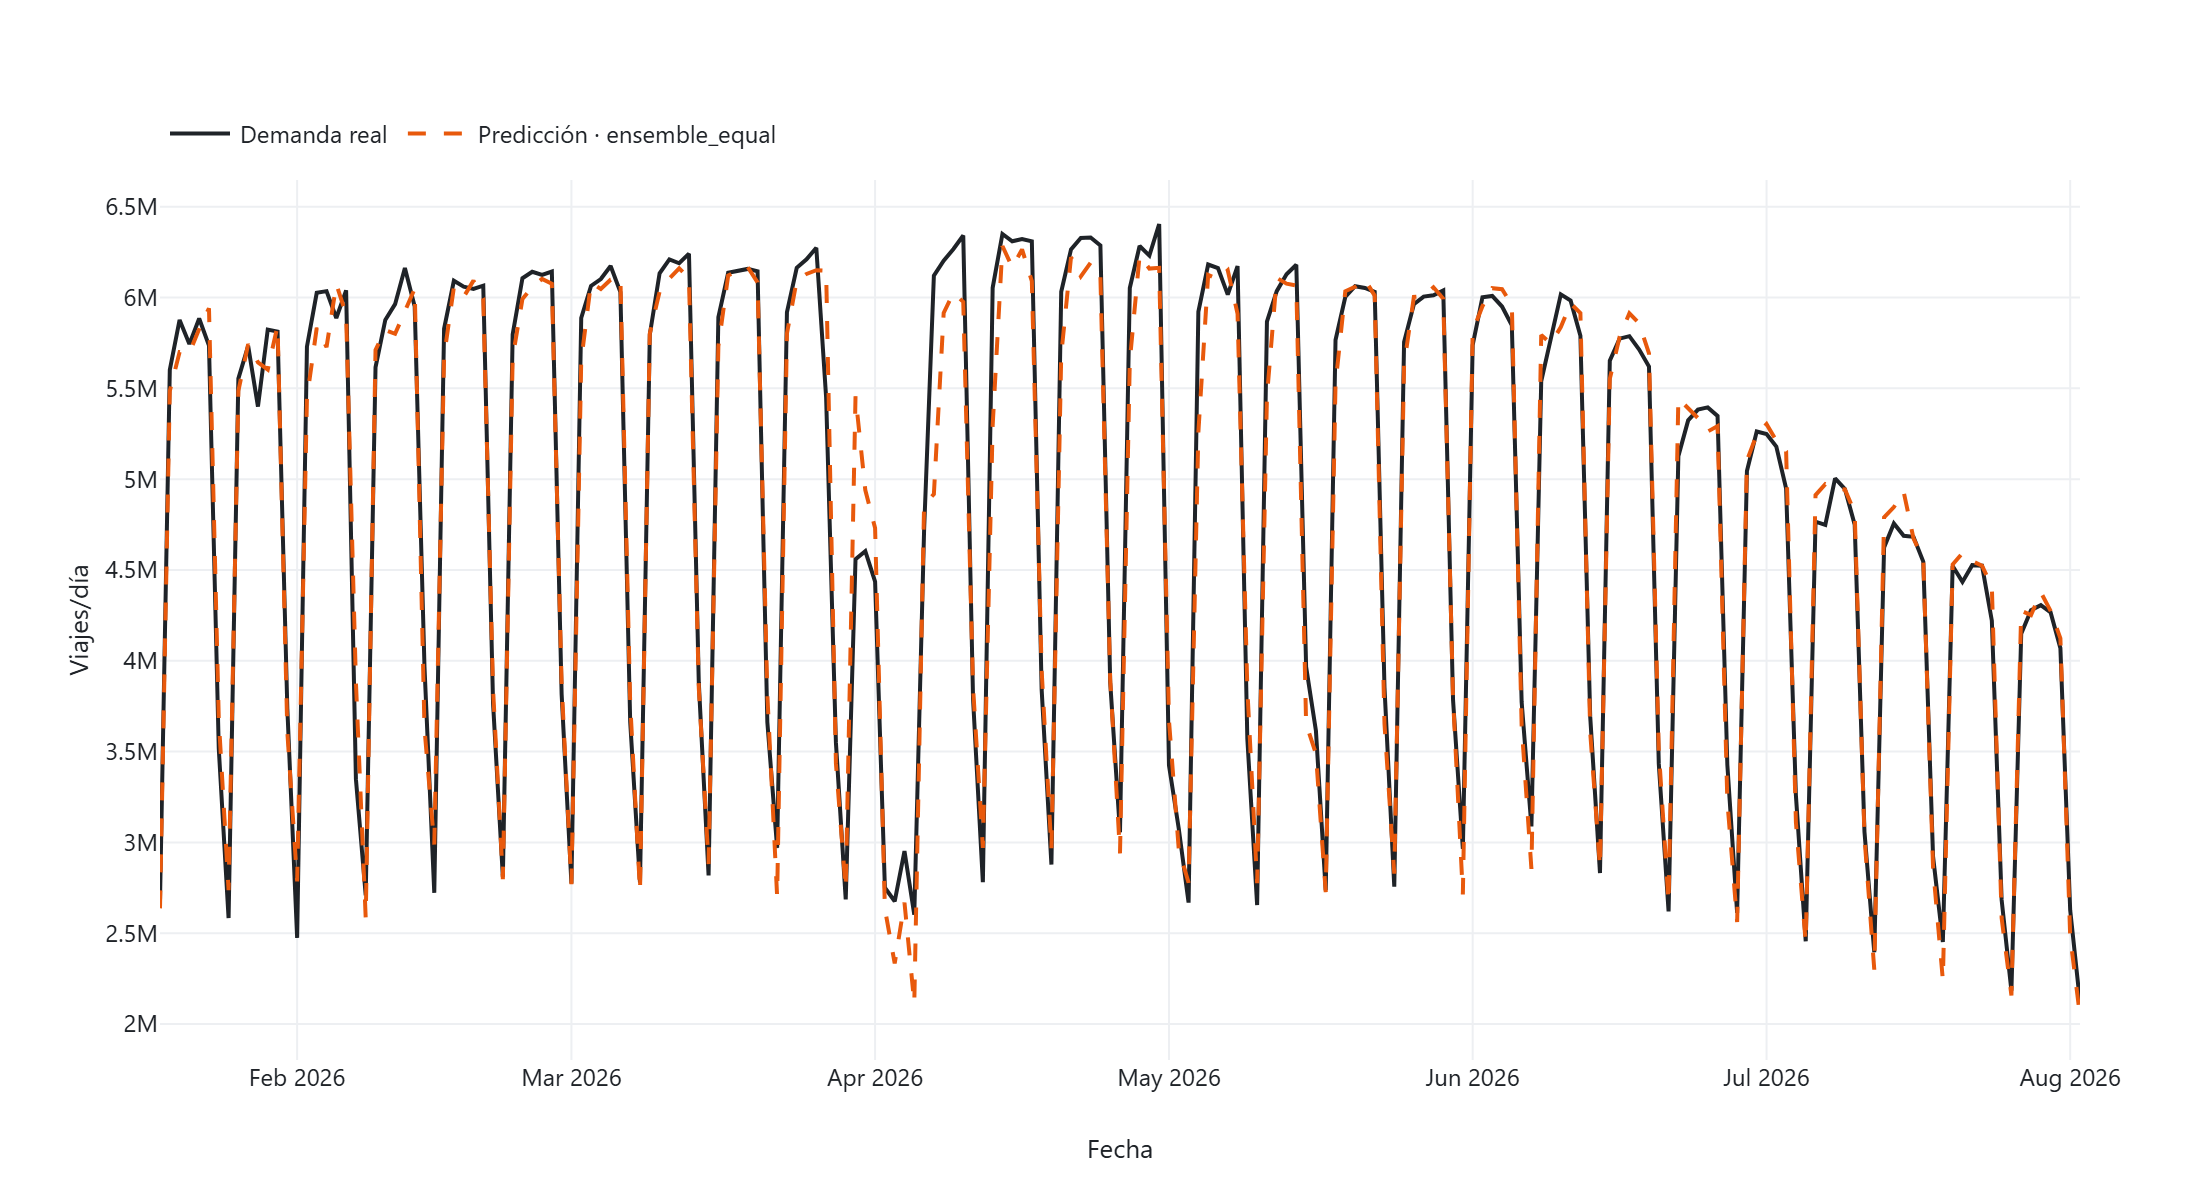
\includegraphics[width=0.78\textwidth]{demand_actual_vs_predicted_test.png}
  \caption{\headlinecolor{Demanda diaria real y predicha por el modelo \texttt{ensemble\_equal} en la partición test. Serie observada y predicha superpuestas.}}
  \label{fig:demand_actual_vs_predicted_test}
\end{figure}

\section{Análisis de residuos}\label{sec:analisis_residuos}

El análisis de residuos permite distinguir un modelo que generaliza de uno que memoriza.
El caso más claro de esta distinción en todo el proyecto es \texttt{xgboost\_alone}: su
coeficiente de determinación en entrenamiento alcanza 0,9929, un ajuste casi perfecto,
frente a un MAE de test de 156.121; esa brecha entre un $R^2$ de entrenamiento
prácticamente unitario y un error de test sustancial es indicativa de que el modelo
memoriza una parte relevante de su conjunto de entrenamiento en lugar de limitarse a
capturar la estructura genuinamente generalizable de la demanda. La figura
\ref{fig:residual_distribution_xgboost_alone} hace visible esta brecha comparando las
distribuciones de error en train y en test: la primera es marcadamente más estrecha y
centrada que la segunda, un patrón de sobreajuste clásico en un modelo de árboles con
capacidad suficiente para ajustar el ruido de una muestra de apenas 889 observaciones
diarias. Es importante subrayar que la cifra que debe citarse en cualquier afirmación
sobre el desempeño de este modelo es siempre la de test, nunca la de entrenamiento como si
fuera indicativa de generalización.

\begin{figure}[htbp]
  \centering
  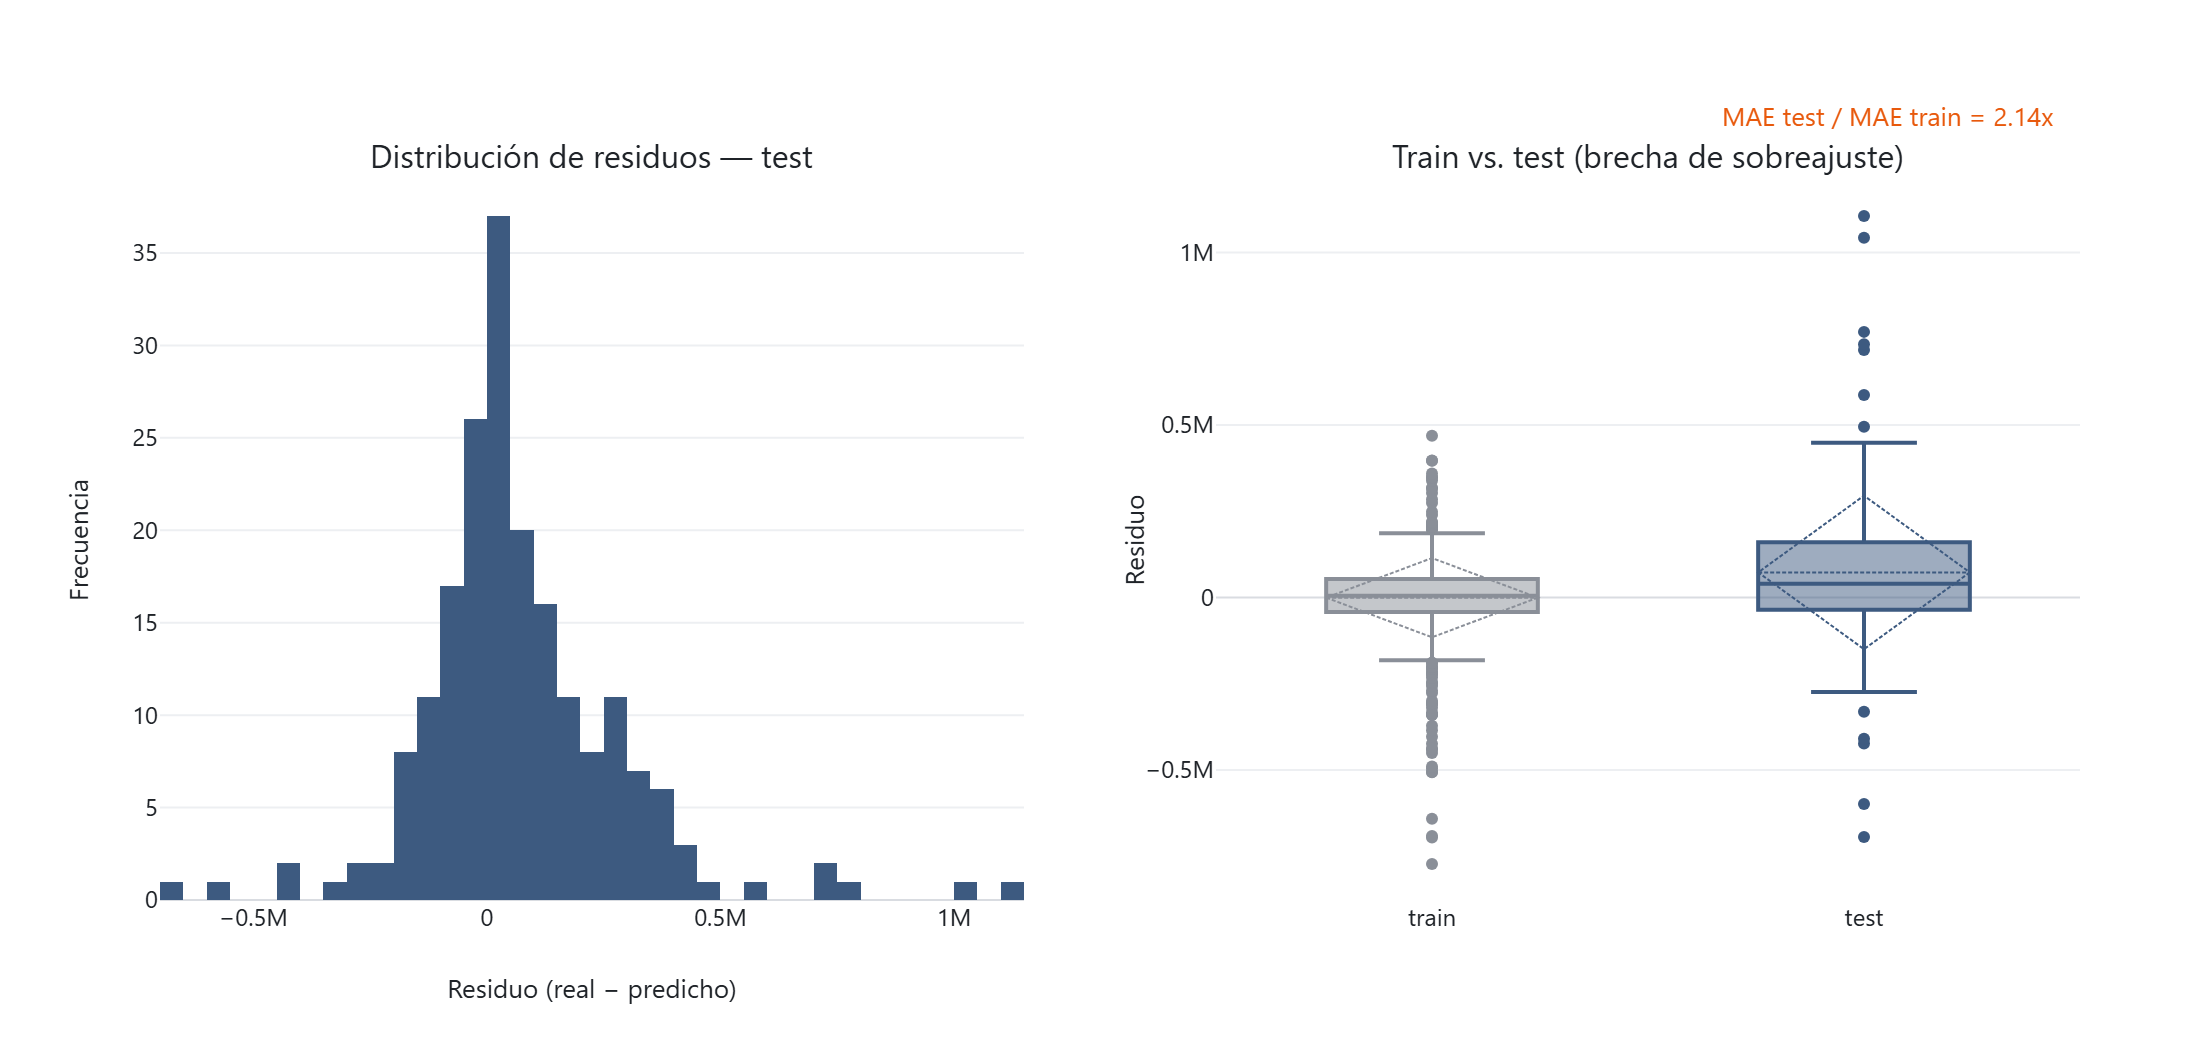
\includegraphics[width=0.78\textwidth]{residual_distribution_xgboost_alone.png}
  \caption{\headlinecolor{Distribución del error de predicción del modelo \texttt{xgboost\_alone} en la partición test. La brecha train-test es la evidencia visual del sobreajuste ($R^2$ train = 0,9929 frente a MAE test = 156.121).}}
  \label{fig:residual_distribution_xgboost_alone}
\end{figure}

Los modelos derivados de la etapa 1 LSTM, \texttt{hybrid} entre ellos, no disponen de esta
misma comparación train-test, puesto que la fase 4 únicamente persistió predicciones del
modelo final sobre las particiones de validación y de test, no sobre entrenamiento; no se
fuerza aquí una comparación que los datos disponibles no permiten. La
figura \ref{fig:residual_distribution_hybrid} muestra, en su lugar, la distribución del
error de \texttt{hybrid} en test sin más: una distribución visiblemente más dispersa que
la de \texttt{xgboost\_alone}, coherente con el MAE de test casi 50\,\% mayor que se
cuantificó en la sección \ref{sec:tabla_maestra}.

\begin{figure}[htbp]
  \centering
  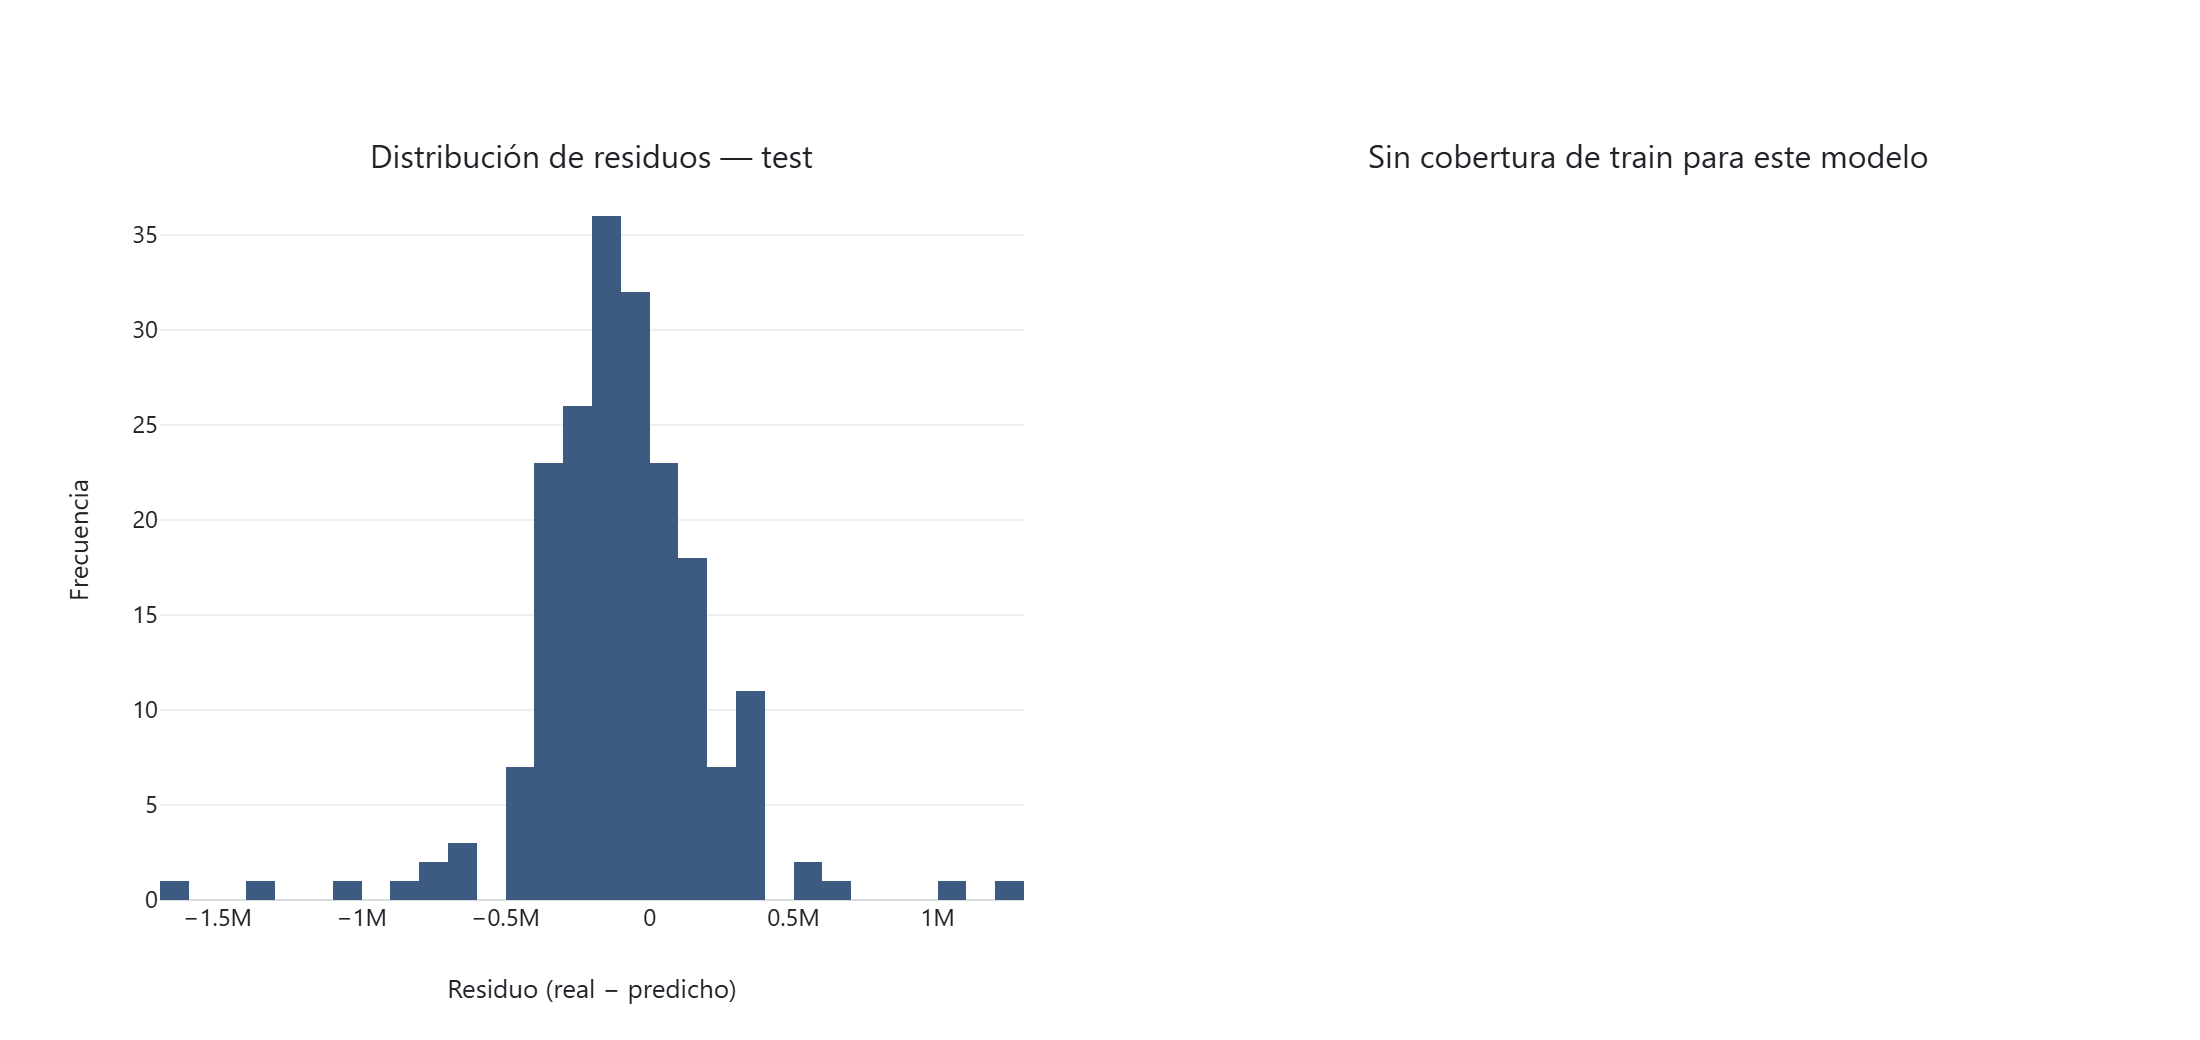
\includegraphics[width=0.78\textwidth]{residual_distribution_hybrid.png}
  \caption{\headlinecolor{Distribución del error de predicción del modelo \texttt{hybrid} en la partición test.}}
  \label{fig:residual_distribution_hybrid}
\end{figure}

Por contraste, la figura \ref{fig:residual_distribution_ensemble_equal} muestra la
distribución de error del modelo ganador, \texttt{ensemble\_equal}: una distribución
sensiblemente más estrecha y mejor centrada en torno a cero que la de cualquiera de sus
dos componentes individuales por separado. Este estrechamiento es coherente con el
mecanismo de reducción de varianza por descorrelación de errores que se cuantifica en la
sección \ref{sec:mecanismo_ensemble}: promediar dos modelos cuyos errores no están
perfectamente correlacionados produce un error agregado con menor dispersión que
cualquiera de los dos errores originales, incluso sin que ninguno de los dos componentes
cambie en absoluto.

\begin{figure}[htbp]
  \centering
  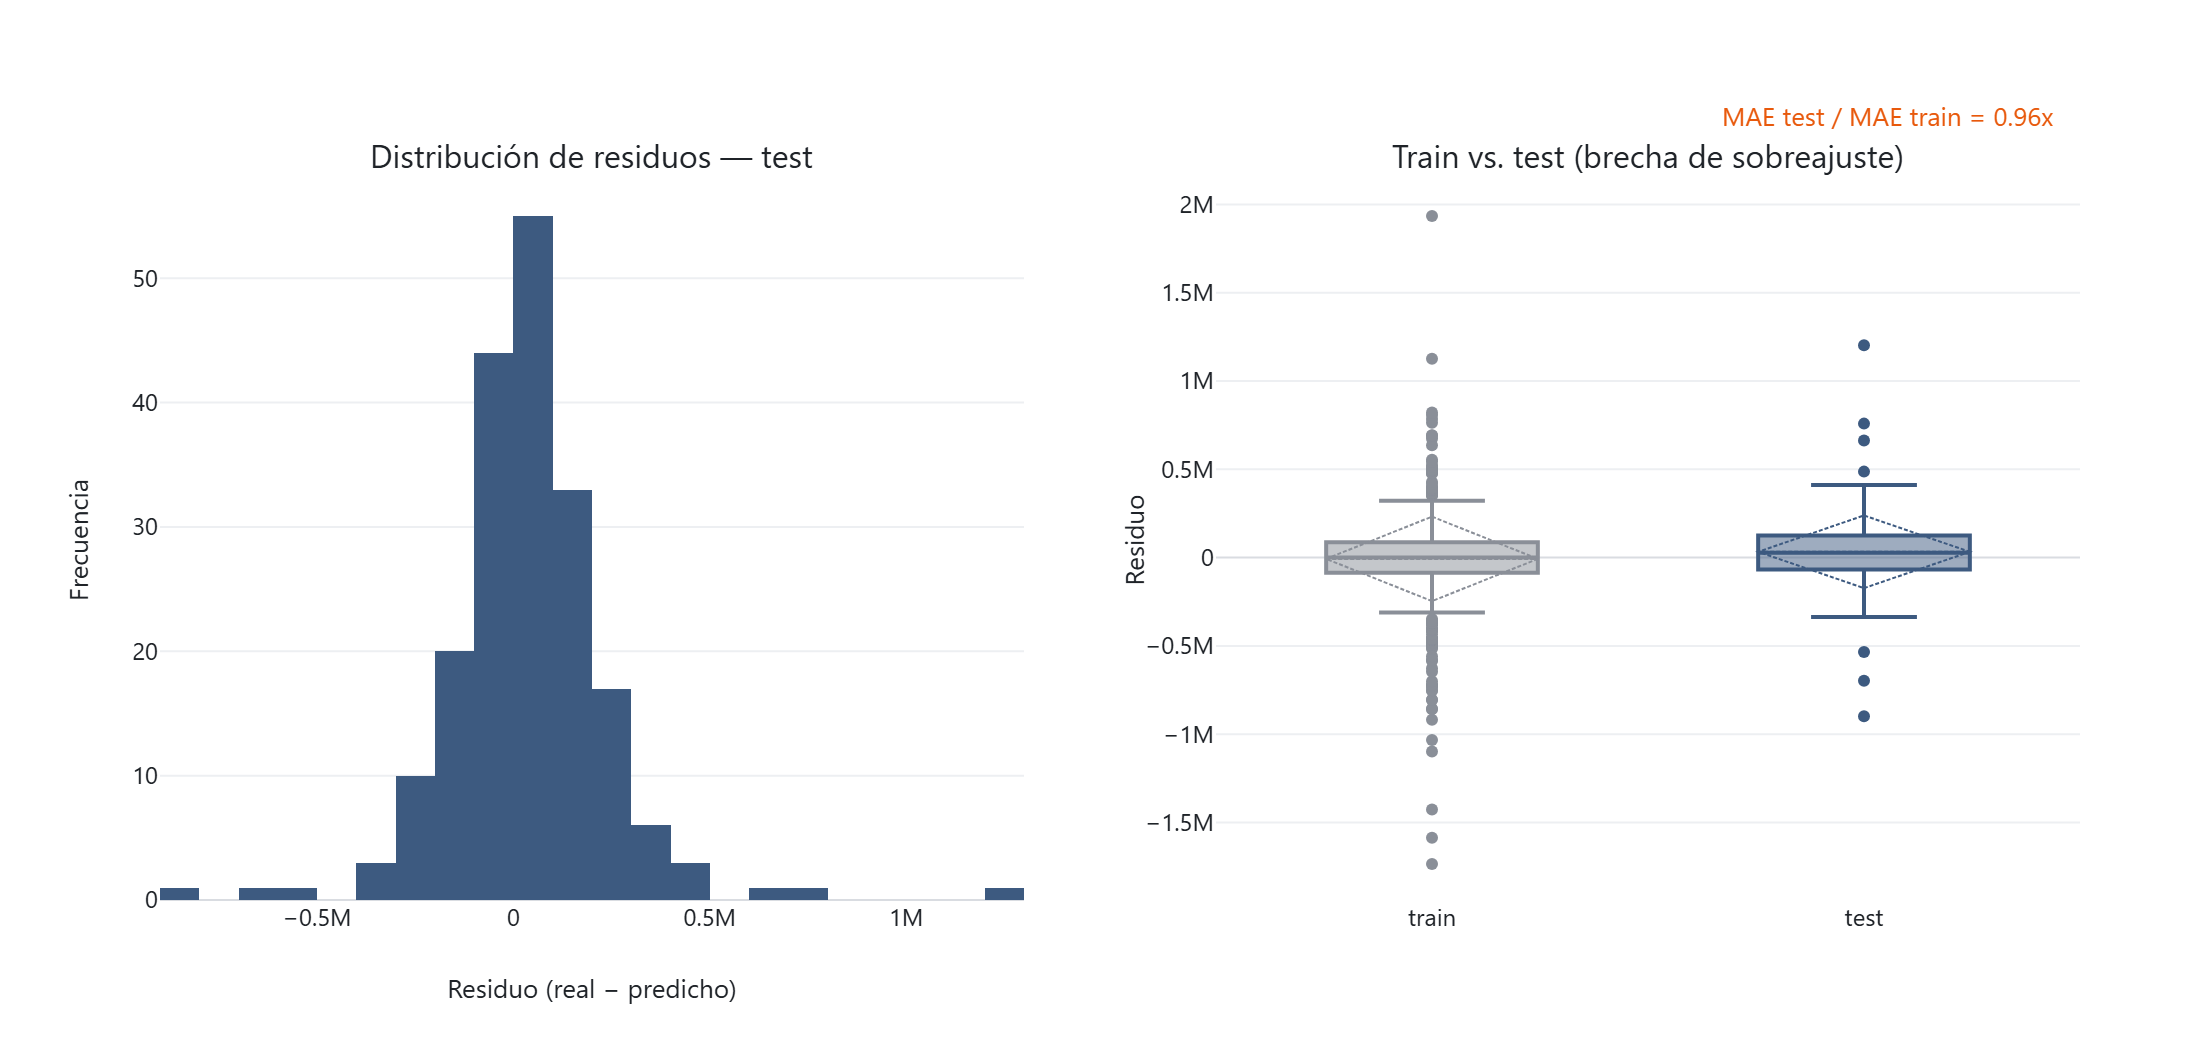
\includegraphics[width=0.78\textwidth]{residual_distribution_ensemble_equal.png}
  \caption{\headlinecolor{Distribución del error de predicción del modelo \texttt{ensemble\_equal} (ganador) en la partición test.}}
  \label{fig:residual_distribution_ensemble_equal}
\end{figure}

\section{Error por tipo de día}\label{sec:error_dia}

Las tablas \ref{tab:desglose_dia_test} y \ref{tab:desglose_dia_val} descomponen el MAE de
cada modelo por régimen de calendario (laborable ordinario, laborable con puente, sábado,
domingo y festivo), y la figura \ref{fig:error_by_day_type_test} lo representa
gráficamente, atenuando visualmente los
grupos con menos de diez observaciones y anotando su tamaño muestral bajo cada barra. La
sección \ref{sec:desglose_subgrupos} retoma esta descomposición de forma sistemática
(quince subgrupos de calendario y periodo fijados por adelantado, con réplica en validación
y corrección por comparaciones múltiples) para responder a si el híbrido mejora en algún
régimen concreto.

\begin{table}[htbp]
  \centering
  \small
  \begin{tabular}{>{\raggedright\arraybackslash}p{2.6cm}>{\centering\arraybackslash}p{0.7cm}>{\centering\arraybackslash}p{1.7cm}>{\centering\arraybackslash}p{1.9cm}>{\centering\arraybackslash}p{1.6cm}>{\centering\arraybackslash}p{1.9cm}>{\centering\arraybackslash}p{1.9cm}}
\toprule
\rowcolor{naranja}
\textbf{Tipo de día} & \textbf{n} & \textbf{sarimax} & \textbf{xgboost\_\allowbreak{}alone} & \textbf{hybrid} & \textbf{hybrid\_\allowbreak{}weighted} & \textbf{ensemble\_\allowbreak{}equal} \\
\midrule
\rowcolor{filaclara} Laborable ordinario & 133 & 148.297 & 169.488 & 211.581 & 200.326 & 138.628 \\
Laborable & 136 & 150.493 & 169.845 & 215.729 & 205.438 & 140.352 \\
\rowcolor{filaclara} Sábado & 27 & 203.910 & 129.381 & 247.793 & 185.918 & 138.805 \\
Domingo & 29 & 169.129 & 100.200 & 233.778 & 243.096 & 122.591 \\
\rowcolor{filaclara} Festivo & 5 & 271.410 & 251.553 & 666.572 & 677.429 & 227.037 \\
Laborable, puente & 3 & 247.865 & 185.671 & 399.637 & 432.066 & 216.768 \\
\bottomrule
\end{tabular}

  \caption{\headlinecolor{MAE por tipo de día, partición test. n=5 (festivo) y n=3 (laborable, puente): indicativos, no concluyentes. La fila ``Laborable'' ($n=136$) es la suma de ``Laborable ordinario'' (133) y ``Laborable, puente'' (3); no es un grupo adicional independiente.}}
  \label{tab:desglose_dia_test}
\end{table}

\begin{table}[htbp]
  \centering
  \small
  \begin{tabular}{>{\raggedright\arraybackslash}p{2.6cm}>{\centering\arraybackslash}p{0.7cm}>{\centering\arraybackslash}p{1.7cm}>{\centering\arraybackslash}p{1.9cm}>{\centering\arraybackslash}p{1.6cm}>{\centering\arraybackslash}p{1.9cm}>{\centering\arraybackslash}p{1.9cm}}
\toprule
\rowcolor{naranja}
\textbf{Tipo de día} & \textbf{n} & \textbf{sarimax} & \textbf{xgboost\_\allowbreak{}alone} & \textbf{hybrid} & \textbf{hybrid\_\allowbreak{}weighted} & \textbf{ensemble\_\allowbreak{}equal} \\
\midrule
\rowcolor{filaclara} Laborable ordinario & 121 & 211.578 & 263.817 & 242.993 & 240.264 & 205.597 \\
Laborable & 133 & 238.197 & 285.078 & 286.849 & 280.851 & 231.011 \\
\rowcolor{filaclara} Sábado & 26 & 435.186 & 132.334 & 278.593 & 245.120 & 246.171 \\
Domingo & 28 & 245.694 & 128.658 & 245.450 & 253.547 & 162.840 \\
\rowcolor{filaclara} Festivo & 9 & 413.907 & 336.750 & 306.409 & 370.935 & 324.760 \\
Laborable, puente & 12 & 506.603 & 499.452 & 729.068 & 690.105 & 487.269 \\
\bottomrule
\end{tabular}

  \caption{\headlinecolor{MAE por tipo de día, partición val. La fila ``Laborable'' ($n=133$) es la suma de ``Laborable ordinario'' (121) y ``Laborable, puente'' (12); no es un grupo adicional independiente.}}
  \label{tab:desglose_dia_val}
\end{table}

Esta descomposición revela la razón mecánica por la que el ensamble supera a ambos
modelos de una sola etapa que lo componen, y no solo el hecho de que lo hace. Sobre la
partición test, SARIMAX es claramente mejor que \texttt{xgboost\_alone} en los días
laborables ordinarios (MAE 148.297 frente a 169.488): su componente autorregresivo
estacional captura con precisión la dinámica de la inmensa mayoría de los días del año,
que son precisamente laborables ordinarios. \texttt{xgboost\_alone}, en cambio, es
netamente superior en fin de semana: en domingo su MAE es 100.200 frente a los 169.129 de
SARIMAX, y en sábado 129.381 frente a 203.910, casi 40\,\% y 37\,\% mejor,
respectivamente. \textbf{Ningún modelo domina al otro de forma global}; cada uno acierta mejor en
un subconjunto distinto y complementario de los días del año, y es exactamente esa
complementariedad la que hace mecánicamente ventajoso promediarlos, como se formaliza en
la sección \ref{sec:mecanismo_ensemble}.

El híbrido y su variante reponderada no participan de esta complementariedad: son, con la
única excepción de la comparación frente a \texttt{lstm\_alone}, peores que SARIMAX y que
\texttt{xgboost\_alone} en prácticamente todos los grupos de la tabla
\ref{tab:desglose_dia_test}. El hallazgo parcialmente positivo, y el único genuinamente
favorable a la arquitectura híbrida en todo ese desglose, aparece en festivos: la etapa 2
reduce el error de su propia etapa 1 de 1.585.388 (fila festivo, columna
\texttt{lstm\_alone} de la tabla \ref{tab:desglose_dia_test}) a 666.572, una mejora del
58\,\%, que muestra de nuevo que
el mecanismo de corrección funciona como está diseñado. Aun así, ese 666.572 sigue siendo
2,5 veces peor que el MAE de SARIMAX en el mismo grupo (271.410) y notablemente peor que
\texttt{xgboost\_alone} (251.553): la corrección funciona, pero parte de una etapa 1
demasiado débil como para que el resultado corregido alcance a los modelos de una sola
etapa.

\begin{figure}[htbp]
  \centering
  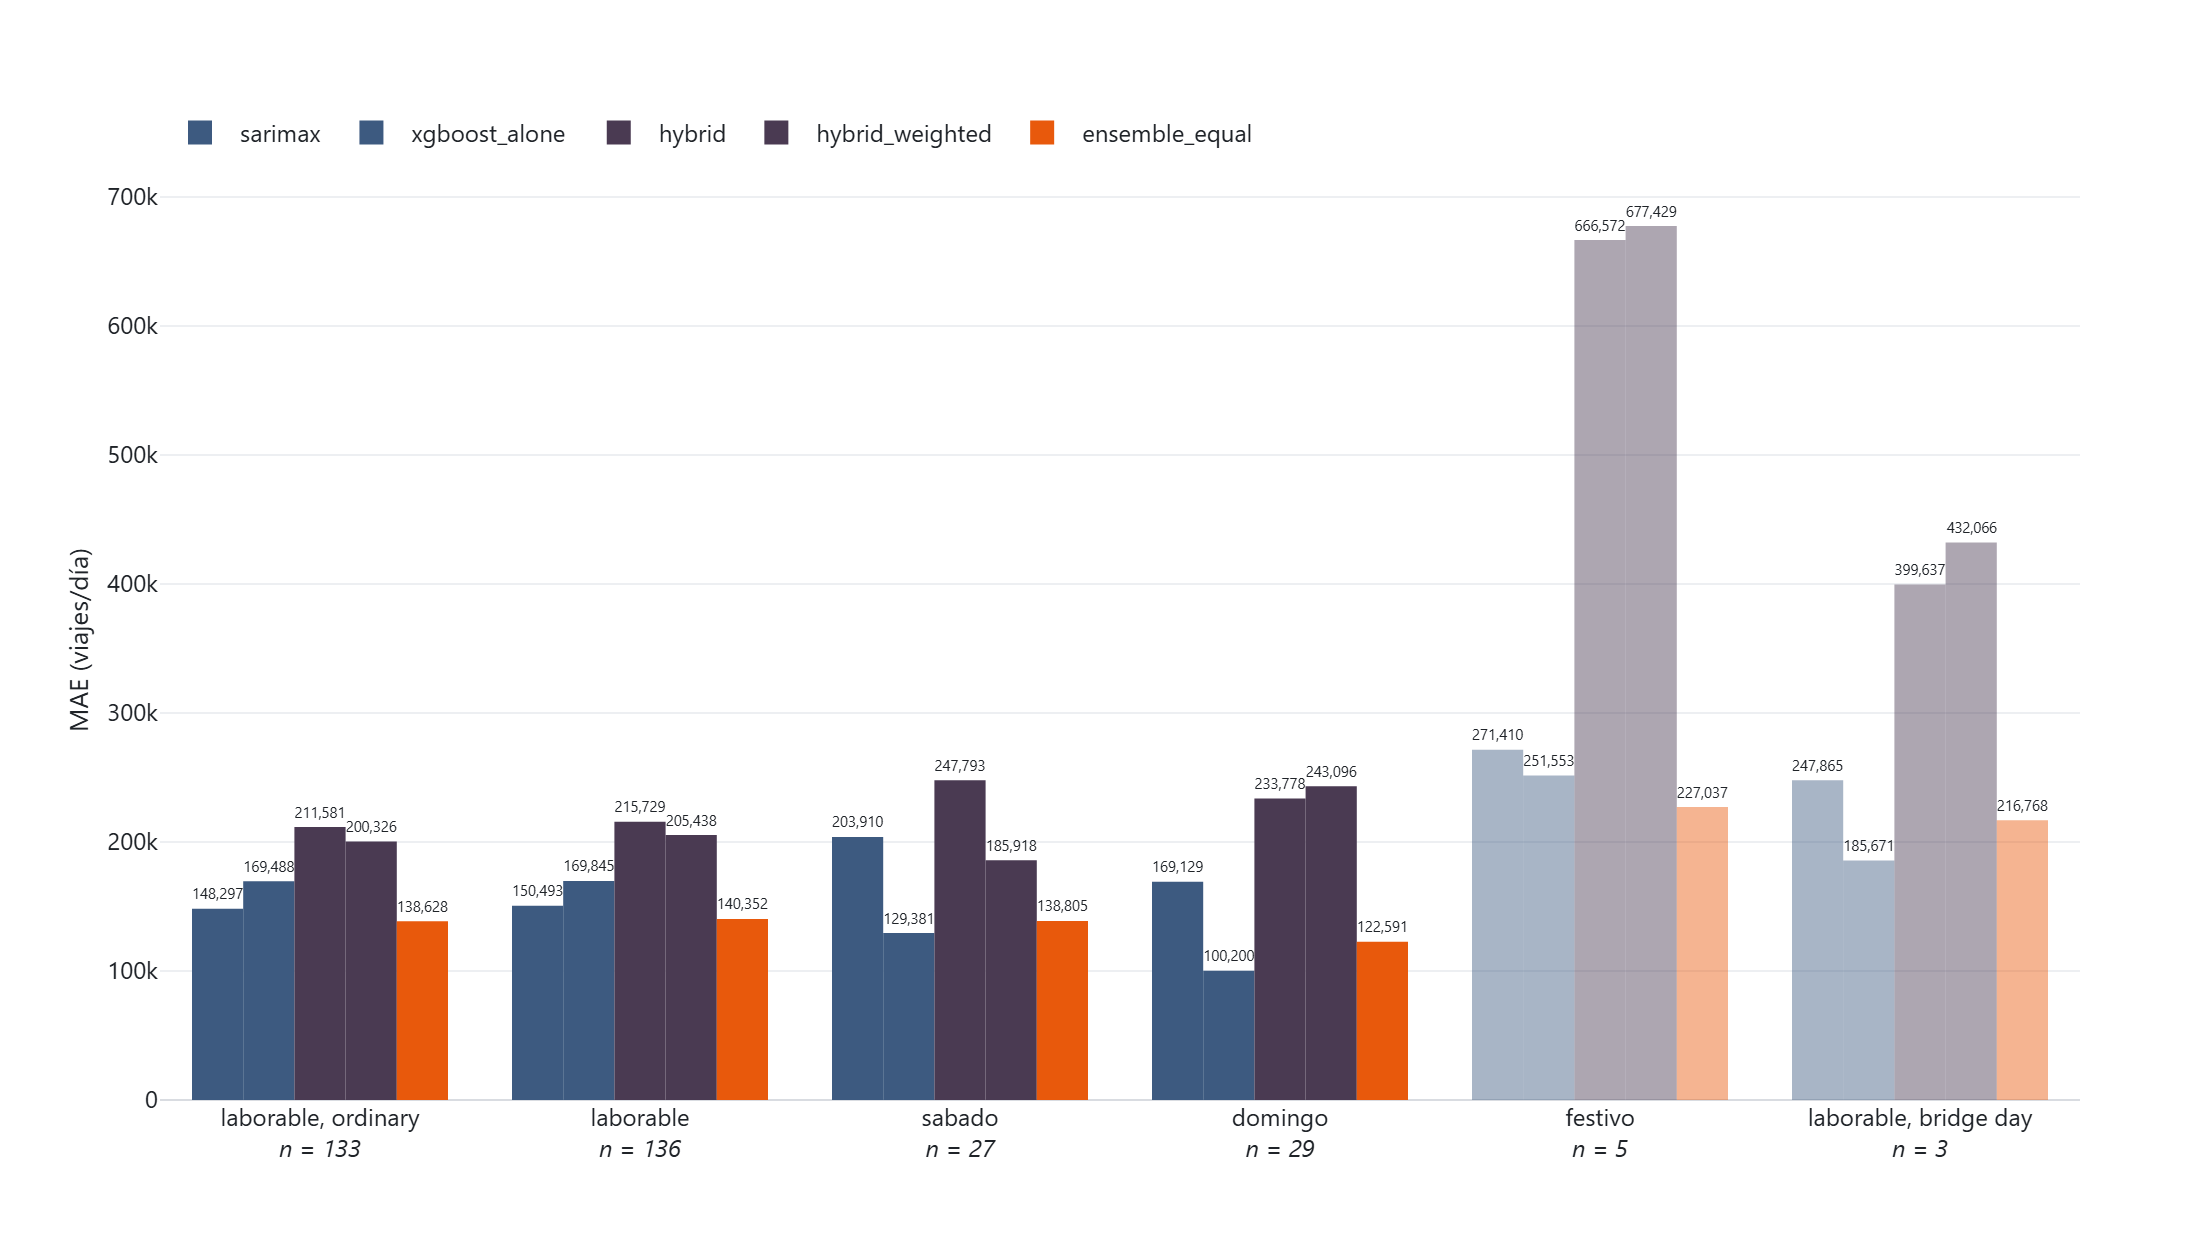
\includegraphics[width=0.78\textwidth]{error_by_day_type_test.png}
  \caption{\headlinecolor{MAE por tipo de día en la partición test. Los grupos con $n < 10$ se dibujan con opacidad reducida y su n anotado bajo el eje: son indicativos, no concluyentes.}}
  \label{fig:error_by_day_type_test}
\end{figure}

Es indispensable acompañar toda esta lectura de una nota de cautela obligatoria: en la
partición test, el grupo de festivos contiene únicamente cinco observaciones y el de
laborables con puente solo tres. Con muestras de ese tamaño, un único día atípico puede
desplazar el MAE del grupo entero en cientos de miles de viajes, de modo que estas dos
filas deben leerse como indicativas y en ningún caso como concluyentes; para afirmaciones
robustas sobre \emph{dónde} se concentra estructuralmente el error de un modelo univariante
frente al calendario, la base más sólida sigue siendo el diagnóstico exploratorio de la
fase 4 sobre el periodo completo (48 festivos y 54 puentes; la codificación de
calendario detecta 55 días puente sobre el total de 1.310 días, de los que 54 quedan
fuera de los 28 días de calentamiento excluidos del entrenamiento), no las particiones
reducidas de test y validación empleadas para esta comparación final.

\section{Importancia de variables}\label{sec:importancia_variables}

Las figuras \ref{fig:feature_importance_group_xgboost_alone} y
\ref{fig:feature_importance_group_xgboost_residual}, junto con las tablas
\ref{tab:importancia_grupo_alone} y \ref{tab:importancia_grupo_residual}, agregan la
ganancia de cada uno de los dos modelos XGBoost del proyecto por grupo temático de
variable, y las tablas \ref{tab:top15_alone} y \ref{tab:top15_residual} descienden al
detalle de las quince variables individuales más influyentes de cada modelo. El contraste entre ambos modelos es la evidencia más directa
de todo el capítulo sobre qué tipo de información resuelve cada problema de predicción.

\begin{figure}[htbp]
  \centering
  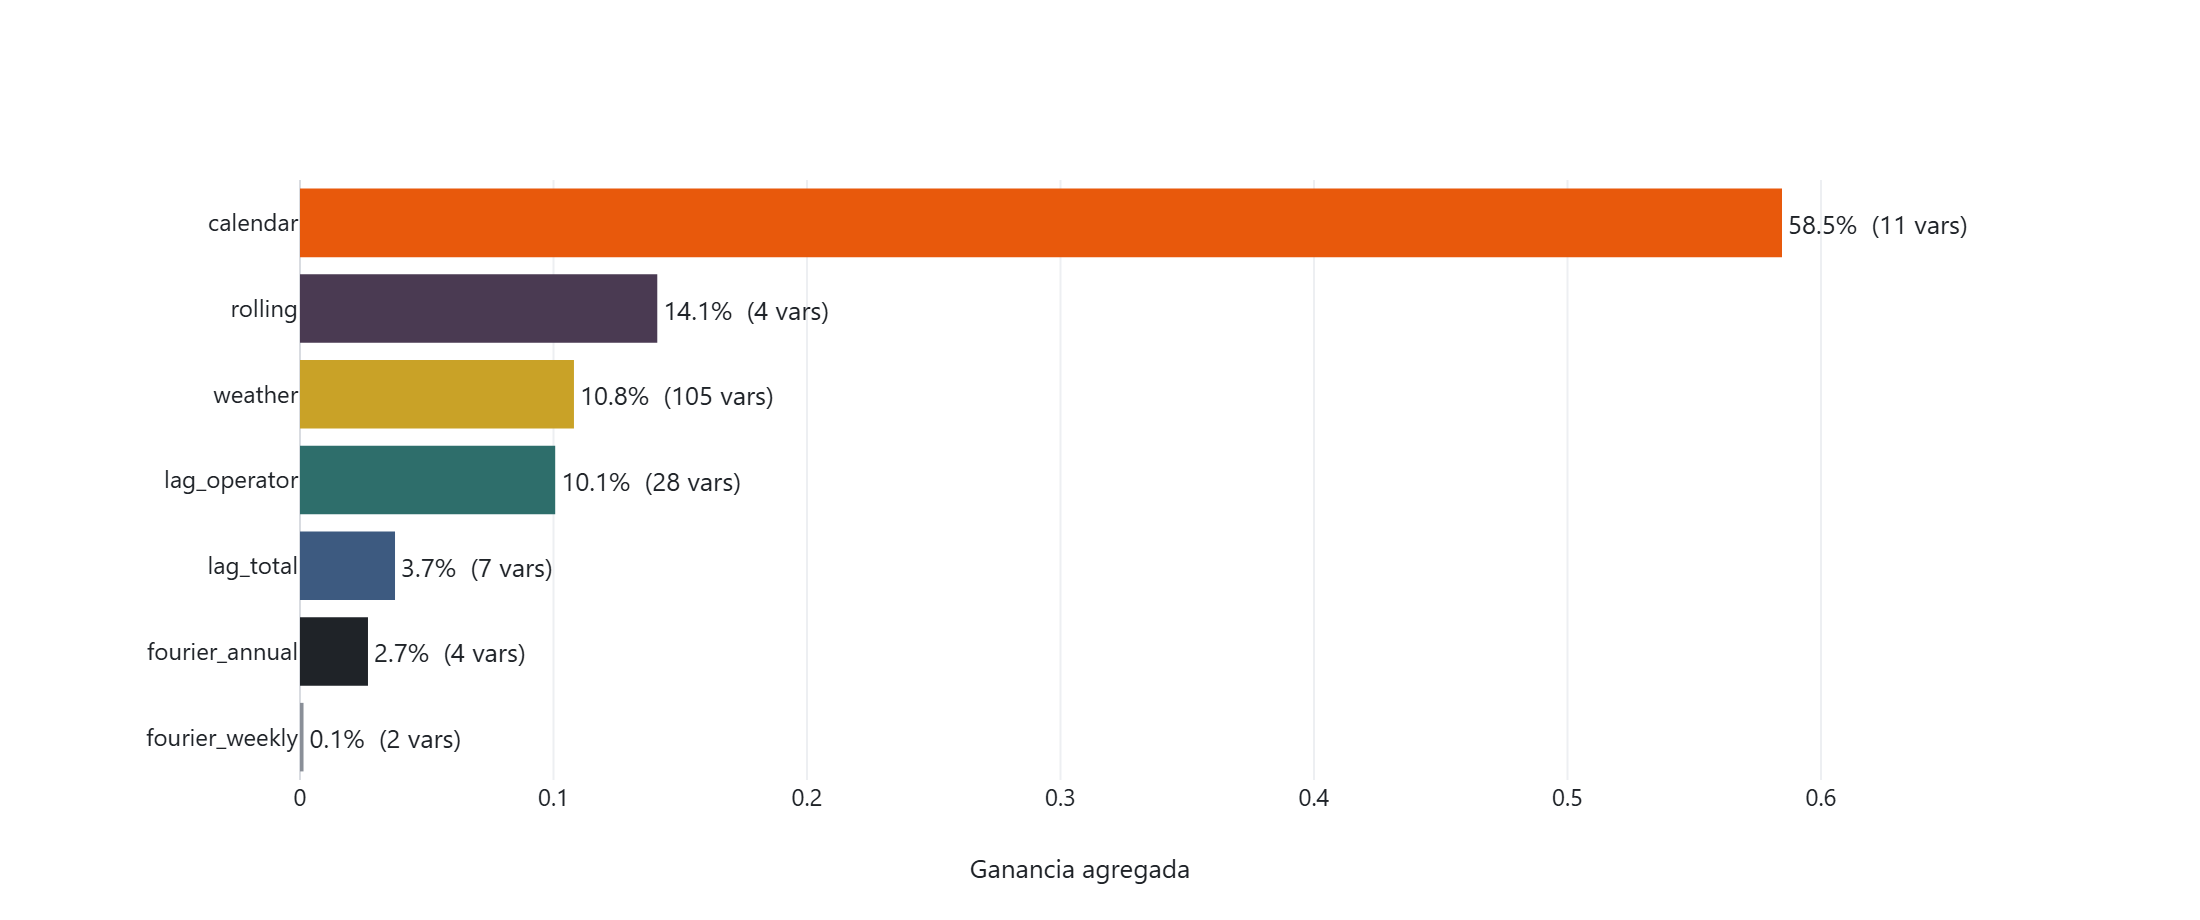
\includegraphics[width=0.78\textwidth]{feature_importance_group_xgboost_alone.png}
  \caption{\headlinecolor{Importancia agregada por grupo de variables del modelo \texttt{xgboost\_alone}, medida como ganancia.}}
  \label{fig:feature_importance_group_xgboost_alone}
\end{figure}

En \texttt{xgboost\_alone}, el grupo de calendario, solo 11 de las 161 variables
disponibles, concentra el 58,5\,\% de la ganancia total del modelo (tabla
\ref{tab:importancia_grupo_alone}), y su variable individual más influyente con
diferencia, \texttt{feat\_day\_type\_laborable}, aporta por sí sola una ganancia de
0,561 (tabla \ref{tab:top15_alone}): al predecir la demanda directamente, saber si el día
es laborable resuelve la práctica totalidad de la varianza semanal identificada en la
sección \ref{sec:eda}, y el resto de variables (retardos de operador, meteorología
retardada, términos de Fourier) se reparten un papel claramente secundario de matiz fino
sobre ese nivel base.

\begin{table}[htbp]
  \centering
  \small
  \begin{tabular}{lrrr}
\toprule
\rowcolor{naranja}
\textbf{Grupo} & \textbf{N.º variables} & \textbf{Ganancia} & \textbf{Peso (\%)} \\
\midrule
\rowcolor{filaclara} calendar & 11 & 0,5846 & 58,46 \\
rolling & 4 & 0,1409 & 14,09 \\
\rowcolor{filaclara} weather & 105 & 0,1081 & 10,81 \\
lag\_\allowbreak{}operator & 28 & 0,1007 & 10,07 \\
\rowcolor{filaclara} lag\_\allowbreak{}total & 7 & 0,0375 & 3,75 \\
fourier\_\allowbreak{}annual & 4 & 0,0268 & 2,68 \\
\rowcolor{filaclara} fourier\_\allowbreak{}weekly & 2 & 0,0014 & 0,14 \\
\bottomrule
\end{tabular}

  \caption{\headlinecolor{Importancia por grupo de variables, \texttt{xgboost\_alone}.}}
  \label{tab:importancia_grupo_alone}
\end{table}

\begin{table}[htbp]
  \centering
  \small
  \begin{tabular}{rllr}
\toprule
\rowcolor{naranja}
\textbf{\#} & \textbf{Variable} & \textbf{Grupo} & \textbf{Ganancia} \\
\midrule
\rowcolor{filaclara} 1 & feat\_\allowbreak{}day\_\allowbreak{}type\_\allowbreak{}laborable & calendar & 0,5609 \\
2 & feat\_\allowbreak{}total\_\allowbreak{}roll\_\allowbreak{}std\_\allowbreak{}7 & rolling & 0,1321 \\
\rowcolor{filaclara} 3 & feat\_\allowbreak{}carretera\_\allowbreak{}lag\_\allowbreak{}1 & lag\_\allowbreak{}operator & 0,0209 \\
4 & feat\_\allowbreak{}total\_\allowbreak{}lag\_\allowbreak{}1 & lag\_\allowbreak{}total & 0,0157 \\
\rowcolor{filaclara} 5 & feat\_\allowbreak{}day\_\allowbreak{}type\_\allowbreak{}sabado & calendar & 0,0156 \\
6 & feat\_\allowbreak{}metro\_\allowbreak{}lag\_\allowbreak{}1 & lag\_\allowbreak{}operator & 0,0152 \\
\rowcolor{filaclara} 7 & feat\_\allowbreak{}metro\_\allowbreak{}lag\_\allowbreak{}14 & lag\_\allowbreak{}operator & 0,0134 \\
8 & feat\_\allowbreak{}fourier\_\allowbreak{}annual\_\allowbreak{}k2\_\allowbreak{}sin & fourier\_\allowbreak{}annual & 0,0127 \\
\rowcolor{filaclara} 9 & feat\_\allowbreak{}relative\_\allowbreak{}humidity\_\allowbreak{}2m\_\allowbreak{}mean\_\allowbreak{}lag\_\allowbreak{}2 & weather & 0,0111 \\
10 & feat\_\allowbreak{}emt\_\allowbreak{}lag\_\allowbreak{}1 & lag\_\allowbreak{}operator & 0,0110 \\
\rowcolor{filaclara} 11 & feat\_\allowbreak{}apparent\_\allowbreak{}temperature\_\allowbreak{}min\_\allowbreak{}lag\_\allowbreak{}1 & weather & 0,0086 \\
12 & feat\_\allowbreak{}total\_\allowbreak{}lag\_\allowbreak{}3 & lag\_\allowbreak{}total & 0,0075 \\
\rowcolor{filaclara} 13 & feat\_\allowbreak{}is\_\allowbreak{}bridge\_\allowbreak{}day & calendar & 0,0070 \\
14 & feat\_\allowbreak{}relative\_\allowbreak{}humidity\_\allowbreak{}2m\_\allowbreak{}mean\_\allowbreak{}roll\_\allowbreak{}mean\_\allowbreak{}7 & weather & 0,0064 \\
\rowcolor{filaclara} 15 & feat\_\allowbreak{}fourier\_\allowbreak{}annual\_\allowbreak{}k1\_\allowbreak{}cos & fourier\_\allowbreak{}annual & 0,0060 \\
\bottomrule
\end{tabular}

  \caption{\headlinecolor{Top-15 variables individuales por ganancia, \texttt{xgboost\_alone}.}}
  \label{tab:top15_alone}
\end{table}

El modelo residual de la etapa 2, \texttt{xgboost\_residual}, invierte por completo esta
jerarquía de grupos (figura \ref{fig:feature_importance_group_xgboost_residual}, tabla
\ref{tab:importancia_grupo_residual}): la meteorología retardada, con sus 105 variables,
concentra ahora el 51,6\,\% de la ganancia, mientras que el calendario desciende al
17,3\,\%, prácticamente empatado con los retardos de operador (17,2\,\%). La lectura
inmediata de esta inversión, y la que se adoptó al observarla por primera vez, es
coherente con la propia definición de la variable objetivo de esta etapa: el residuo
$e_t = y_t - \hat y^{\text{LSTM}}_t$ ya no contendría la componente de calendario más
gruesa, la distinción laborable/fin de semana, porque una parte relevante de esa
componente ya habría sido absorbida, con mayor o menor acierto, por la propia dinámica
temporal de la etapa 1; lo que quedaría por explicar en el residuo sería, en consecuencia,
un matiz más fino, y ese matiz estaría más ligado a las condiciones meteorológicas
retardadas que al calendario grueso.

Conviene subrayar que esto es una \emph{hipótesis}
sugerida por una clasificación de importancia, no un resultado medido, y que las fases
diagnósticas la someten a prueba con dos análisis independientes y la \textbf{rechazan}:
la sección \ref{sec:residuo_meteo_anatomia} no encuentra ninguna correlación parcial
significativa entre el residuo y las 105 variables meteorológicas retardadas, y la
ablación de la sección \ref{sec:ablacion_bloques} muestra que retirar ese bloque
\emph{mejora} el modelo. La sección \ref{sec:lectura_conjunta} reconcilia esa aparente
contradicción y explica por qué una cuota de ganancia elevada es perfectamente compatible
con la ausencia de señal aprovechable.

\begin{figure}[htbp]
  \centering
  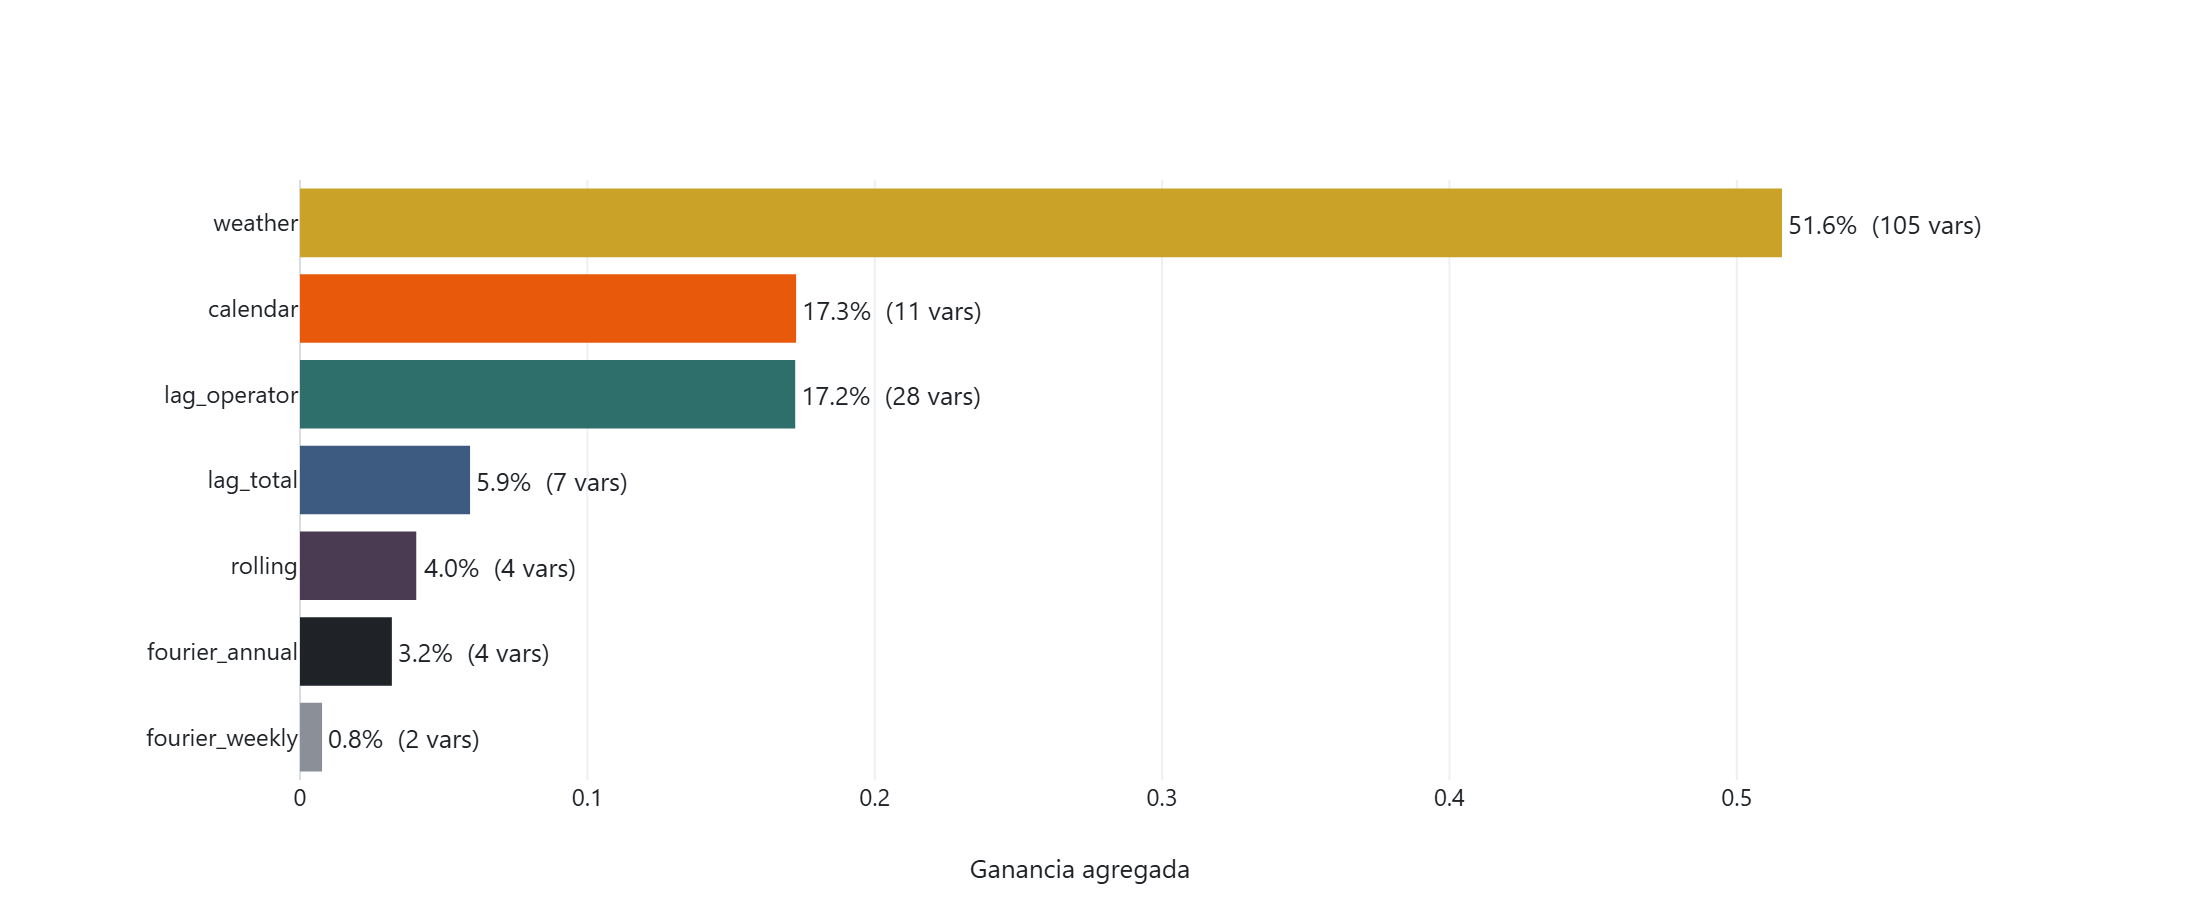
\includegraphics[width=0.78\textwidth]{feature_importance_group_xgboost_residual.png}
  \caption{\headlinecolor{Importancia agregada por grupo de variables del modelo \texttt{xgboost\_\allowbreak{}residual} (etapa 2 del híbrido).}}
  \label{fig:feature_importance_group_xgboost_residual}
\end{figure}

\begin{table}[htbp]
  \centering
  \small
  \begin{tabular}{lrrr}
\toprule
\rowcolor{naranja}
\textbf{Grupo} & \textbf{N.º variables} & \textbf{Ganancia} & \textbf{Peso (\%)} \\
\midrule
\rowcolor{filaclara} weather & 105 & 0,5157 & 51,57 \\
calendar & 11 & 0,1726 & 17,26 \\
\rowcolor{filaclara} lag\_\allowbreak{}operator & 28 & 0,1723 & 17,23 \\
lag\_\allowbreak{}total & 7 & 0,0592 & 5,92 \\
\rowcolor{filaclara} rolling & 4 & 0,0405 & 4,05 \\
fourier\_\allowbreak{}annual & 4 & 0,0320 & 3,20 \\
\rowcolor{filaclara} fourier\_\allowbreak{}weekly & 2 & 0,0077 & 0,77 \\
\bottomrule
\end{tabular}

  \caption{\headlinecolor{Importancia por grupo de variables, \texttt{xgboost\_residual}.}}
  \label{tab:importancia_grupo_residual}
\end{table}

Sin embargo, esta relectura por grupo no contradice el hallazgo mecanístico más
importante de la etapa 2, visible únicamente al bajar al nivel de variable individual
(tabla \ref{tab:top15_residual}): pese a que el calendario pesa menos como grupo agregado,
la variable individual con mayor ganancia en todo el modelo residual sigue siendo
\texttt{feat\_day\_type\_festivo}, con una ganancia de 0,125, muy por delante de la
segunda variable de la lista. Esto es coherente, al nivel de variable individual, con que la
etapa 2 aprenda la señal de calendario (en concreto, la irregularidad de los festivos) que
la etapa 1 univariante no puede ver por construcción: el mecanismo que justifica
teóricamente la arquitectura híbrida se manifiesta en la variable que cabría esperar, con
independencia de que el veredicto agregado de la
sección \ref{sec:contraste_central} termine siendo negativo para la arquitectura completa.

\begin{table}[htbp]
  \centering
  \small
  \begin{tabular}{rllr}
\toprule
\rowcolor{naranja}
\textbf{\#} & \textbf{Variable} & \textbf{Grupo} & \textbf{Ganancia} \\
\midrule
\rowcolor{filaclara} 1 & feat\_\allowbreak{}day\_\allowbreak{}type\_\allowbreak{}festivo & calendar & 0,1254 \\
2 & feat\_\allowbreak{}apparent\_\allowbreak{}temperature\_\allowbreak{}max\_\allowbreak{}lag\_\allowbreak{}7 & weather & 0,0759 \\
\rowcolor{filaclara} 3 & feat\_\allowbreak{}temperature\_\allowbreak{}2m\_\allowbreak{}mean\_\allowbreak{}lag\_\allowbreak{}3 & weather & 0,0337 \\
4 & feat\_\allowbreak{}carretera\_\allowbreak{}lag\_\allowbreak{}3 & lag\_\allowbreak{}operator & 0,0319 \\
\rowcolor{filaclara} 5 & feat\_\allowbreak{}day\_\allowbreak{}type\_\allowbreak{}laborable & calendar & 0,0305 \\
6 & feat\_\allowbreak{}total\_\allowbreak{}lag\_\allowbreak{}7 & lag\_\allowbreak{}total & 0,0249 \\
\rowcolor{filaclara} 7 & feat\_\allowbreak{}total\_\allowbreak{}roll\_\allowbreak{}std\_\allowbreak{}28 & rolling & 0,0217 \\
8 & feat\_\allowbreak{}apparent\_\allowbreak{}temperature\_\allowbreak{}min\_\allowbreak{}lag\_\allowbreak{}3 & weather & 0,0200 \\
\rowcolor{filaclara} 9 & feat\_\allowbreak{}apparent\_\allowbreak{}temperature\_\allowbreak{}max\_\allowbreak{}lag\_\allowbreak{}3 & weather & 0,0191 \\
10 & feat\_\allowbreak{}temperature\_\allowbreak{}2m\_\allowbreak{}min\_\allowbreak{}roll\_\allowbreak{}mean\_\allowbreak{}7 & weather & 0,0189 \\
\rowcolor{filaclara} 11 & feat\_\allowbreak{}weather\_\allowbreak{}code\_\allowbreak{}roll\_\allowbreak{}mean\_\allowbreak{}7 & weather & 0,0152 \\
12 & feat\_\allowbreak{}metro\_\allowbreak{}lag\_\allowbreak{}7 & lag\_\allowbreak{}operator & 0,0152 \\
\rowcolor{filaclara} 13 & feat\_\allowbreak{}shortwave\_\allowbreak{}radiation\_\allowbreak{}sum\_\allowbreak{}roll\_\allowbreak{}mean\_\allowbreak{}7 & weather & 0,0149 \\
14 & feat\_\allowbreak{}total\_\allowbreak{}lag\_\allowbreak{}28 & lag\_\allowbreak{}total & 0,0137 \\
\rowcolor{filaclara} 15 & feat\_\allowbreak{}temperature\_\allowbreak{}2m\_\allowbreak{}max\_\allowbreak{}roll\_\allowbreak{}mean\_\allowbreak{}7 & weather & 0,0128 \\
\bottomrule
\end{tabular}

  \caption{\headlinecolor{Top-15 variables individuales por ganancia, \texttt{xgboost\_residual}. \texttt{feat\_\allowbreak{}day\_\allowbreak{}type\_\allowbreak{}festivo} encabeza con ganancia 0,125 -- coherente con que la etapa 2 aprenda la señal de calendario que la etapa 1 no puede ver.}}
  \label{tab:top15_residual}
\end{table}

\section{Contraste central del TFM}\label{sec:contraste_central}

Con la evidencia de las secciones anteriores ya establecida, esta sección responde de
forma explícita a la pregunta que estructura todo el proyecto: ¿mejora la
arquitectura híbrida residual LSTM-XGBoost, tal como se ha diseñado e implementado en
este TFM, la predicción de demanda frente a SARIMAX y frente a un XGBoost entrenado
directamente sobre las mismas variables predictoras? La respuesta, sostenida por la tabla
\ref{tab:delta_hibrido}, es \textbf{no, en ninguna de las dos comparaciones y en ninguna
de las dos particiones de evaluación}.

\begin{table}[htbp]
  \centering
  \begin{tabular}{llrl}
\toprule
\rowcolor{naranja}
\textbf{Partición} & \textbf{Comparación} & \textbf{Delta MAE} & \textbf{Veredicto} \\
\midrule
\rowcolor{filaclara} val & hybrid - sarimax & 7.270 & hybrid peor \\
val & hybrid - xgboost\_\allowbreak{}alone & 35.895 & hybrid peor \\
\rowcolor{filaclara} test & hybrid - sarimax & 70.597 & hybrid peor \\
test & hybrid - xgboost\_\allowbreak{}alone & 78.103 & hybrid peor \\
\bottomrule
\end{tabular}

  \caption{\headlinecolor{Diferencia de MAE del híbrido frente a SARIMAX y XGBoost independiente (Delta MAE = \texttt{hybrid} $-$ competidor; positivo = híbrido peor). Generada, no introducida manualmente.}}
  \label{tab:delta_hibrido}
\end{table}

Sobre la partición test, el híbrido supera en MAE a SARIMAX en 70.597 viajes diarios y a
\texttt{xgboost\_alone} en 78.103; sobre validación las diferencias son menores en
magnitud absoluta, pero mantienen el mismo signo, 7.270 y 35.895 respectivamente. La
diferencia frente a \texttt{xgboost\_alone} es, en ambas particiones, mayor que la
diferencia frente a SARIMAX: el híbrido no solo pierde frente al baseline estadístico
clásico, sino que pierde por un margen todavía más amplio frente a un modelo de
aprendizaje automático que utiliza exactamente la misma matriz de variables predictoras
sin pasar por ninguna etapa LSTM. Este segundo resultado es el más informativo de los dos: si
el problema fuera únicamente que SARIMAX es un modelo particularmente bien ajustado a esta
serie, cabría esperar que el híbrido, con acceso a variables no lineales y a una capa de
aprendizaje profundo, cerrara al menos parte de esa distancia frente a otro modelo de
aprendizaje automático; en su lugar, la distancia se amplía.

\subsection{Por qué pierde el híbrido: lectura a la luz de Granger (1989)}\label{sec:resultado_negativo_teoria}

La teoría clásica de combinación de pronósticos ofrece un marco preciso para interpretar
este resultado, en lugar de limitarse a documentarlo. \textcite{granger1989combining},
revisando dos décadas de literatura sobre combinación de modelos, formula la condición que
determina cuándo un pronóstico híbrido o combinado puede superar a sus componentes: la
mejora solo es posible cuando los modelos que se combinan son individualmente subóptimos
\emph{y}, de manera crucial, se basan en conjuntos de información distintos entre sí. La
consecuencia de esa condición es que la ganancia de combinar procede de información que
cada componente tiene y el otro no; si el conjunto de información de uno está contenido en
el del otro, la combinación no puede aportar, en teoría, nada que un único modelo sobre el
conjunto mayor no pudiera aprender por sí mismo con una forma funcional suficientemente
flexible.

La arquitectura híbrida de este TFM \textbf{incumple precisamente esa segunda condición}, y
conviene precisar en qué sentido. Los conjuntos de información de las dos etapas no son
idénticos: la etapa 1 observa únicamente la ventana cruda de 28 valores de \texttt{total},
y la etapa 2 dispone además del calendario, la meteorología retardada, los armónicos de
Fourier y los retardos de operador —información que la etapa 1 no ve y que, como muestra
la sección \ref{sec:importancia_variables}, aporta señal genuina; de ahí que la etapa 2
mejore de forma sustancial a su propia etapa 1 (sección \ref{sec:error_dia})—. Pero
tampoco son \emph{distintos} en el sentido que la condición exige: el pasado reciente de la
serie que la etapa 1 observa está representado en la matriz de la etapa 2 por sus siete
retardos y cuatro estadísticos móviles sobre la misma ventana de 28 días, de modo que los
dos conjuntos están, en la práctica, anidados y no son complementarios. En esa situación la
combinación secuencial no puede superar, en teoría, al mejor modelo de una sola etapa sobre
el conjunto mayor, y ese modelo existe en la comparación: \texttt{xgboost\_alone}, que
accede a las mismas 161 variables predictoras sin arrastrar el ruido de una etapa 1
estructuralmente débil. Aunque la segunda etapa incorpora información adicional de
calendario, meteorología retardada y otras variables predictoras, los resultados indican
que esta separación secuencial no genera una complementariedad predictiva suficiente para
compensar el error introducido por la primera etapa LSTM. Los dos controles de la sección
\ref{sec:paridad_informativa} miden ambas mitades de esta lectura: la ablación muestra que
\texttt{xgboost\_alone} extrae por sí mismo la información temporal que la etapa 1 aporta,
y el control de paridad muestra que la vía recurrente no ofrece una representación de ese
pasado que el modelo de una sola etapa no tenga ya.

Esta lectura se refuerza, además, por un factor puramente cuantitativo: la etapa 1
univariante deja un residuo con una desviación típica de 726.669 viajes diarios
(\ref{sec:etapa2_xgboost}), del mismo orden de magnitud que la propia señal que se intenta
predecir. Cuanto mayor es la varianza residual que la segunda etapa debe corregir, más
difícil resulta que esa corrección alcance, y menos aún supere, a un modelo que ataca el
problema completo desde el principio con toda la matriz predictora disponible. Este patrón
—hibridar puede mejorar sustancialmente a un componente débil sin llegar a igualar a un
componente fuerte de una sola etapa cuando sus conjuntos de información están anidados— no
es exclusivo de
este proyecto: es consistente con lo observado de forma sistemática en las competiciones
de pronóstico a gran escala M4 y M5 \parencite{makridakis2018m4,makridakis2022m5}, donde los métodos híbridos y
de combinación que finalmente destacan lo hacen precisamente al combinar familias de
modelos con mecanismos e información de entrada genuinamente distintos, como la propia
sección \ref{sec:mecanismo_ensemble} muestra para el ensamble de este TFM, y no al
encadenar dos etapas sucesivas sobre conjuntos de información anidados. El resultado
negativo del híbrido residual de este TFM debe leerse, por tanto, como consistente con la
teoría publicada y con la evidencia empírica a gran escala, no como una anomalía
específica de esta implementación.

\section{Análisis de sensibilidad}\label{sec:analisis_sensibilidad}

Las dos secciones siguientes documentan dos experimentos acotados y registrados por
adelantado, con su criterio de éxito fijado antes de observar el resultado, diseñados
para explorar el margen de mejora del híbrido y para establecer un punto de comparación
adicional, respectivamente. Ninguno de los dos reabre la conclusión central de la sección
anterior ni constituye una búsqueda de una configuración que la revierta.

\subsection{Experimento A: repesado de días irregulares (3x)}\label{sec:experimento_a}

El primer experimento pregunta si concentrar la capacidad de ajuste de la etapa 2
precisamente en los días de calendario irregular —festivos y puentes, el subconjunto
donde la sección \ref{sec:error_dia} documentó el error relativo más alto de todo el
sistema— mejora el desempeño del híbrido en esos mismos días, a cambio de un coste
acotado en el desempeño global. La variante \texttt{hybrid\_weighted}, descrita en la
sección \ref{sec:modelos_control}, asigna un peso de muestra triple a esas filas (un
8,2\,\% del conjunto residual) sin modificar ningún otro elemento del modelo. El criterio
de éxito, fijado antes de observar el resultado y evaluado mecánicamente en código, exige
el cumplimiento simultáneo de dos condiciones: que el MAE en festivos y puentes mejore, y
que el MAE global de test no empeore más de un 5\,\% frente al híbrido original de la
sección \ref{sec:contraste_central}.

\begin{table}[htbp]
  \centering
  \setlength{\tabcolsep}{4pt}
  \resizebox{\textwidth}{!}{\begin{tabular}{>{\raggedright\arraybackslash}p{6.5cm}>{\centering\arraybackslash}p{1.9cm}>{\centering\arraybackslash}p{2.4cm}>{\centering\arraybackslash}p{3.0cm}}
\toprule
\rowcolor{naranja}
\textbf{Criterio} & \textbf{hybrid} & \textbf{hybrid\_\allowbreak{}weighted} & \textbf{Resultado} \\
\midrule
\rowcolor{filaclara} MAE en días irregulares (festivo + puente), n-ponderado & 566.472 & 585.418 & No mejora \\
MAE global test (techo +5\% sobre 234.223) & 234.223 & 220.286 & Dentro del margen \\
\rowcolor{filaclara} Veredicto del criterio prerregistrado (ambas condiciones) & -- & -- & NO CUMPLIDO \\
\bottomrule
\end{tabular}
}
  \caption{\headlinecolor{Veredicto del criterio prerregistrado del experimento A (repesado 3x de días irregulares). CRITERIO NO CUMPLIDO: el presupuesto global se cumplió pero el error en días irregulares NO mejoró.}}
  \label{tab:criterio_experimento_a}
\end{table}

El veredicto de la tabla \ref{tab:criterio_experimento_a} es que el criterio \textbf{no se
cumple}: la condición de presupuesto global sí se satisface, con un MAE de test que
incluso mejora un 5,95\,\% respecto al híbrido original (234.223 a 220.286), pero el MAE
ponderado por tamaño de muestra en festivos y puentes conjuntamente \emph{empeora}, de
566.472 a 585.418. El aspecto más interesante de este resultado nulo no es que el
repesado fallara, sino \emph{dónde} recayó la mejora que sí se produjo: no en los días que
se pretendía corregir, sino en sábados (mejora del 25\,\%) y en laborables ordinarios
(mejora del 5\,\%). Con solamente 45 filas repesadas frente a 161 variables de entrada, el
peso adicional no parece producir un mejor ajuste específicamente en esas filas; en su
lugar, perturba el ajuste global del modelo, y esa perturbación resulta beneficiar, por
las características propias del conjunto de datos, a los grupos más numerosos en lugar de
a los grupos objetivo. Se reporta como lo que es: un dato sobre la fragilidad del
repesado en muestras pequeñas, no como evidencia a favor ni en contra del esquema de
pesos como estrategia general.

\subsection{Experimento B: ensamble SARIMAX + XGBoost independiente}\label{sec:por_que_ensemble}

El segundo experimento no está sujeto a un criterio de éxito binario, sino que constituye
un punto de comparación que cualquier evaluación rigurosa de este proyecto debe incluir:
¿existe una combinación más sencilla que los propios componentes de una sola etapa? La
respuesta se construye sin ningún reentrenamiento adicional, combinando de forma puramente
aritmética las predicciones de SARIMAX y de \texttt{xgboost\_alone} ya calculadas en las
secciones anteriores, bajo dos esquemas de ponderación (tabla \ref{tab:ensemble_pesos}):
un promedio simple 50/50 (\texttt{ensemble\_equal}) y un promedio ponderado por el inverso
del MAE de validación de cada componente (\texttt{ensemble\_inverse\_mae}).

\begin{table}[htbp]
  \centering
  \begin{tabular}{lrr}
\toprule
\rowcolor{naranja}
\textbf{Variante} & \textbf{Peso SARIMAX} & \textbf{Peso XGBoost-alone} \\
\midrule
\rowcolor{filaclara} ensemble\_\allowbreak{}equal & 0,5000 & 0,5000 \\
ensemble\_\allowbreak{}inverse\_\allowbreak{}mae & 0,4724 & 0,5276 \\
\bottomrule
\end{tabular}

  \caption{\headlinecolor{Pesos de los dos componentes en cada variante del ensamble.}}
  \label{tab:ensemble_pesos}
\end{table}

Como ya adelantó la tabla \ref{tab:comparacion_test}, ambas variantes no solo son
competitivas, sino que \textbf{superan a los dos componentes individuales}; el mecanismo
de esa ganancia se desarrolla en la sección \ref{sec:mecanismo_ensemble}. Los dos esquemas de ponderación producen resultados casi
idénticos entre sí (una diferencia de MAE de test de apenas el 0,03\,\%), lo que no es
sorprendente dado que los pesos óptimos por inverso del MAE, 0,4724 y 0,5276, se sitúan
muy próximos a un reparto igualitario. Por ello, y pese a que \texttt{ensemble\_inverse\_mae}
obtiene el MAE de test nominalmente más bajo de todo el proyecto, se recomienda
\texttt{ensemble\_equal} como modelo de referencia para la memoria: ofrece un
rendimiento prácticamente indistinguible sin necesitar ningún paso de ajuste que
justificar y, a diferencia de la variante ponderada por inverso del MAE —cuyos pesos se
derivan del propio MAE de validación y hacen, por tanto, que su cifra de validación sea
levemente optimista—, no depende en ningún grado de la partición de validación para
fijar sus coeficientes.

\section{Por qué gana el ensamble: descorrelación de errores}\label{sec:mecanismo_ensemble}

La razón mecánica por la que el ensamble supera a ambos componentes individuales, y no
solo el hecho empírico de que lo hace, se puede hacer explícita observando directamente
la relación entre los errores de SARIMAX y de \texttt{xgboost\_alone} en cada día de la
partición test (figura \ref{fig:dispersion_errores}).

\begin{figure}[htbp]
  \centering
  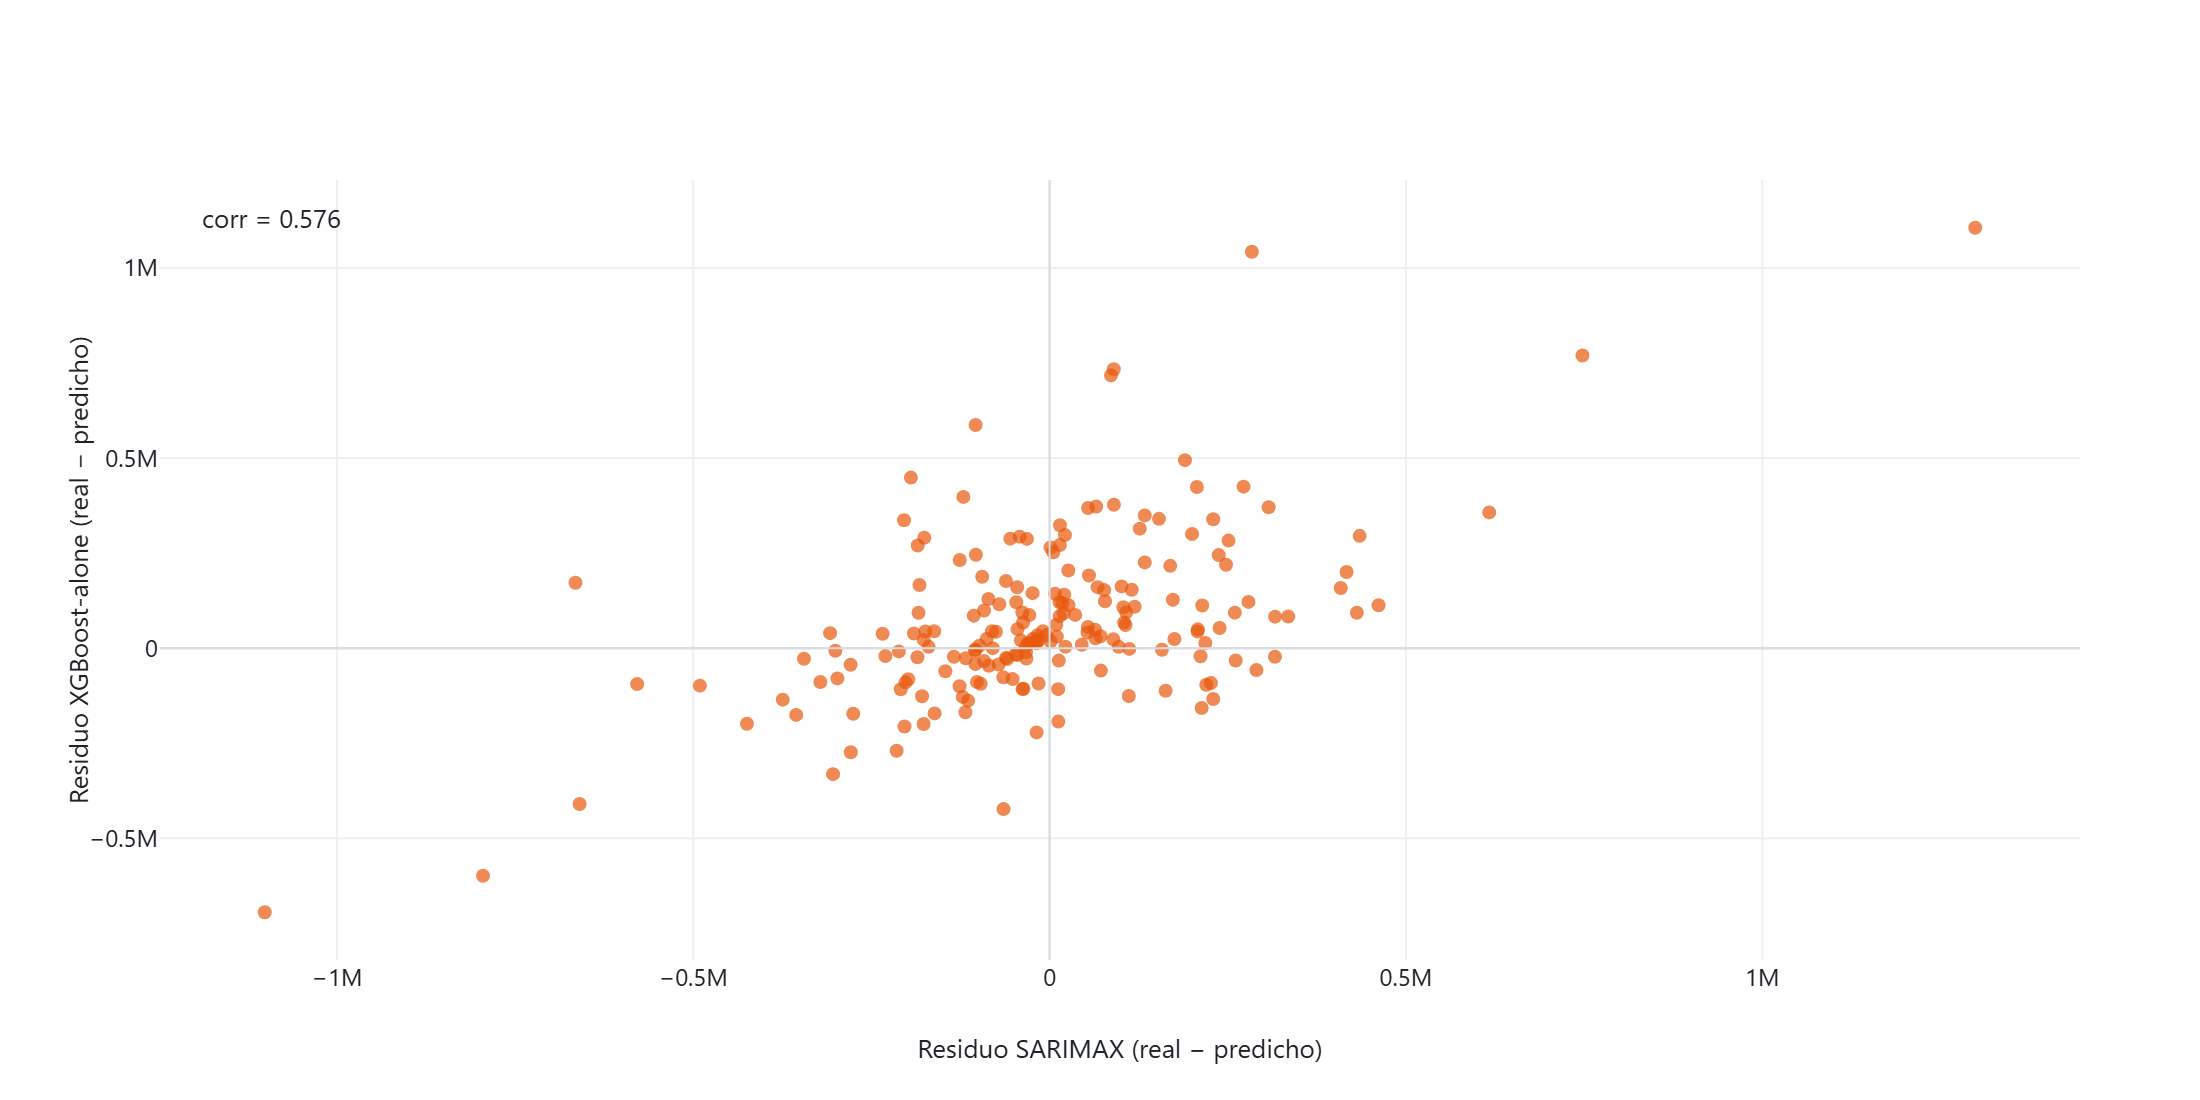
\includegraphics[width=0.78\textwidth]{fig_dispersion_errores_sarimax_xgb.png}
  \caption{\headlinecolor{Dispersión de residuos SARIMAX frente a XGBoost independiente en la partición test -- evidencia mecánica de la reducción de varianza del ensamble (correlación débil entre ambos errores).}}
  \label{fig:dispersion_errores}
\end{figure}

La correlación entre ambos residuos es de 0,576: positiva, como cabría esperar de dos
modelos que atacan el mismo fenómeno subyacente y comparten, por tanto, una parte de su
señal de error, pero claramente inferior a la unidad. Esa distancia respecto a la
correlación perfecta es, precisamente, la que hace mecánicamente ventajoso promediar los
dos modelos. Para dos pronósticos con varianza de error igual $\sigma^2$ y correlación
$\rho$ entre sus errores, la varianza del error de su media aritmética es
\[
  \operatorname{Var}\!\left(\frac{\hat e_1 + \hat e_2}{2}\right)
    = \frac{\sigma^2 (1 + \rho)}{2},
\]
la expresión clásica de la combinación de pronósticos de
\textcite{bates1969combination}: con $\rho = 1$, errores perfectamente correlacionados,
promediar no reduce la varianza en absoluto, mientras que con $\rho = 0{,}576$ la
varianza del error combinado se reduce a aproximadamente el \textbf{79\,\%} de la varianza
individual, incluso bajo el supuesto simplificador de que ambos componentes tuvieran
exactamente el mismo error cuadrático medio. Esta reducción de varianza por promediado de
predictores parcialmente descorrelacionados es, además, el mismo principio que sustenta el
uso de comités o \emph{ensembles} de modelos en el aprendizaje automático en general
\parencite{perrone1993networks}, aplicado aquí no a una colección de redes con la misma
arquitectura sino a dos familias de modelos deliberadamente distintas.

La tabla \ref{tab:desglose_dia_test} explica además por qué esa correlación es
precisamente 0,576 y no un valor más cercano a la unidad: SARIMAX y
\texttt{xgboost\_alone} no cometen simplemente errores de magnitud distinta sobre los
mismos días, sino errores grandes en \emph{días distintos} (el primero en laborables
ordinarios comparativamente, el segundo en fin de semana y festivos), de modo que su
correlación de error refleja una complementariedad estructural de calendario y no solo
ruido estadístico independiente. La ganancia observada, un MAE de test de 139.681 para
\texttt{ensemble\_inverse\_mae}, un 10,5\,\% por debajo del mejor componente individual
(\texttt{xgboost\_alone}, 156.121), es coherente con el mecanismo de reducción de varianza
descrito por Bates y Granger y con la correlación imperfecta observada entre los errores de
SARIMAX y XGBoost; la identidad, formulada en varianza y bajo el supuesto de varianzas
iguales, no la demuestra, pero la ganancia tiene el signo y el orden de magnitud que ese
mecanismo anticipa.

\section{Anatomía del residuo de la etapa 1}\label{sec:anatomia_residuo_etapa1}

La sección \ref{sec:resultado_negativo_teoria} sostuvo, sobre una base teórica, que el
híbrido pierde porque su etapa 1 es un cuello de botella: una LSTM univariante sobre unas
860 observaciones diarias no puede ver el calendario, y la etapa 2 arranca entonces desde
un residuo cuya desviación típica, 555.385 viajes diarios sobre la serie contigua de
validación y test, es del orden de la propia señal. Esta sección deja de afirmarlo y lo
mide. Es un análisis \textbf{confirmatorio, no exploratorio}: que una red que nunca observa
el calendario deje estructura de calendario en su residuo es casi seguro de antemano; la
aportación es cuantificar \emph{cuánta}, con criterios de aceptación fijados en el código
(constantes de módulo de \texttt{stage1\_residual\_anatomy.py}) antes de observar ningún
resultado. Esta sección y las dos siguientes (\ref{sec:paridad_informativa},
\ref{sec:desglose_subgrupos}) son \textbf{controles diagnósticos}: ninguna de sus cifras
entra en la tabla maestra de comparación, en \texttt{dashboard\_data.MODEL\_NAMES} ni en
\texttt{models/}, y ninguna compite por ser el mejor modelo; una prueba por fase
(\texttt{test\_phase7/8/9\_adds\_no\_model\_to\_the\_master\_comparison}) lo fija
mecánicamente. En esta, además, no se entrena, reajusta ni re-predice ningún modelo, con
la única excepción declarada de la curva de aprendizaje de la sección
\ref{sec:tamano_muestral}.

\subsection{Estructura que retiene el residuo}\label{sec:residuo_estructura}

La tabla \ref{tab:autocorrelacion_residuo} y la figura \ref{fig:acf_pacf_residuo} recogen
la autocorrelación del residuo de la etapa 1 hasta cinco ciclos semanales. La memoria
temporal es \textbf{débil y ambigua}: el mayor valor absoluto de la ACF en los retardos 1
a 35 es de solo 0,166 (retardo 28), y aunque cinco de los treinta y cinco retardos quedan
fuera de la banda de Bartlett, frente a los dos que cabría esperar por azar al 5\,\%,
ninguna autocorrelación alcanza el umbral de 0,20 fijado como evidencia de estructura
persistente. El estadístico de Ljung-Box rechaza la hipótesis de ruido blanco en los tres
retardos examinados ($p < 0{,}01$ en 7, 14 y 28), pero esa prueba es
\textbf{anticonservadora} en este contexto —su corrección de grados de libertad no está
definida para una LSTM sin recuento de parámetros significativo, y sobre un residuo
visiblemente autocorrelacionado rechaza con facilidad—, de modo que ninguna afirmación de
esta sección descansa en su valor $p$: el criterio primario es siempre el tamaño del
efecto.

\begin{figure}[htbp]
  \centering
  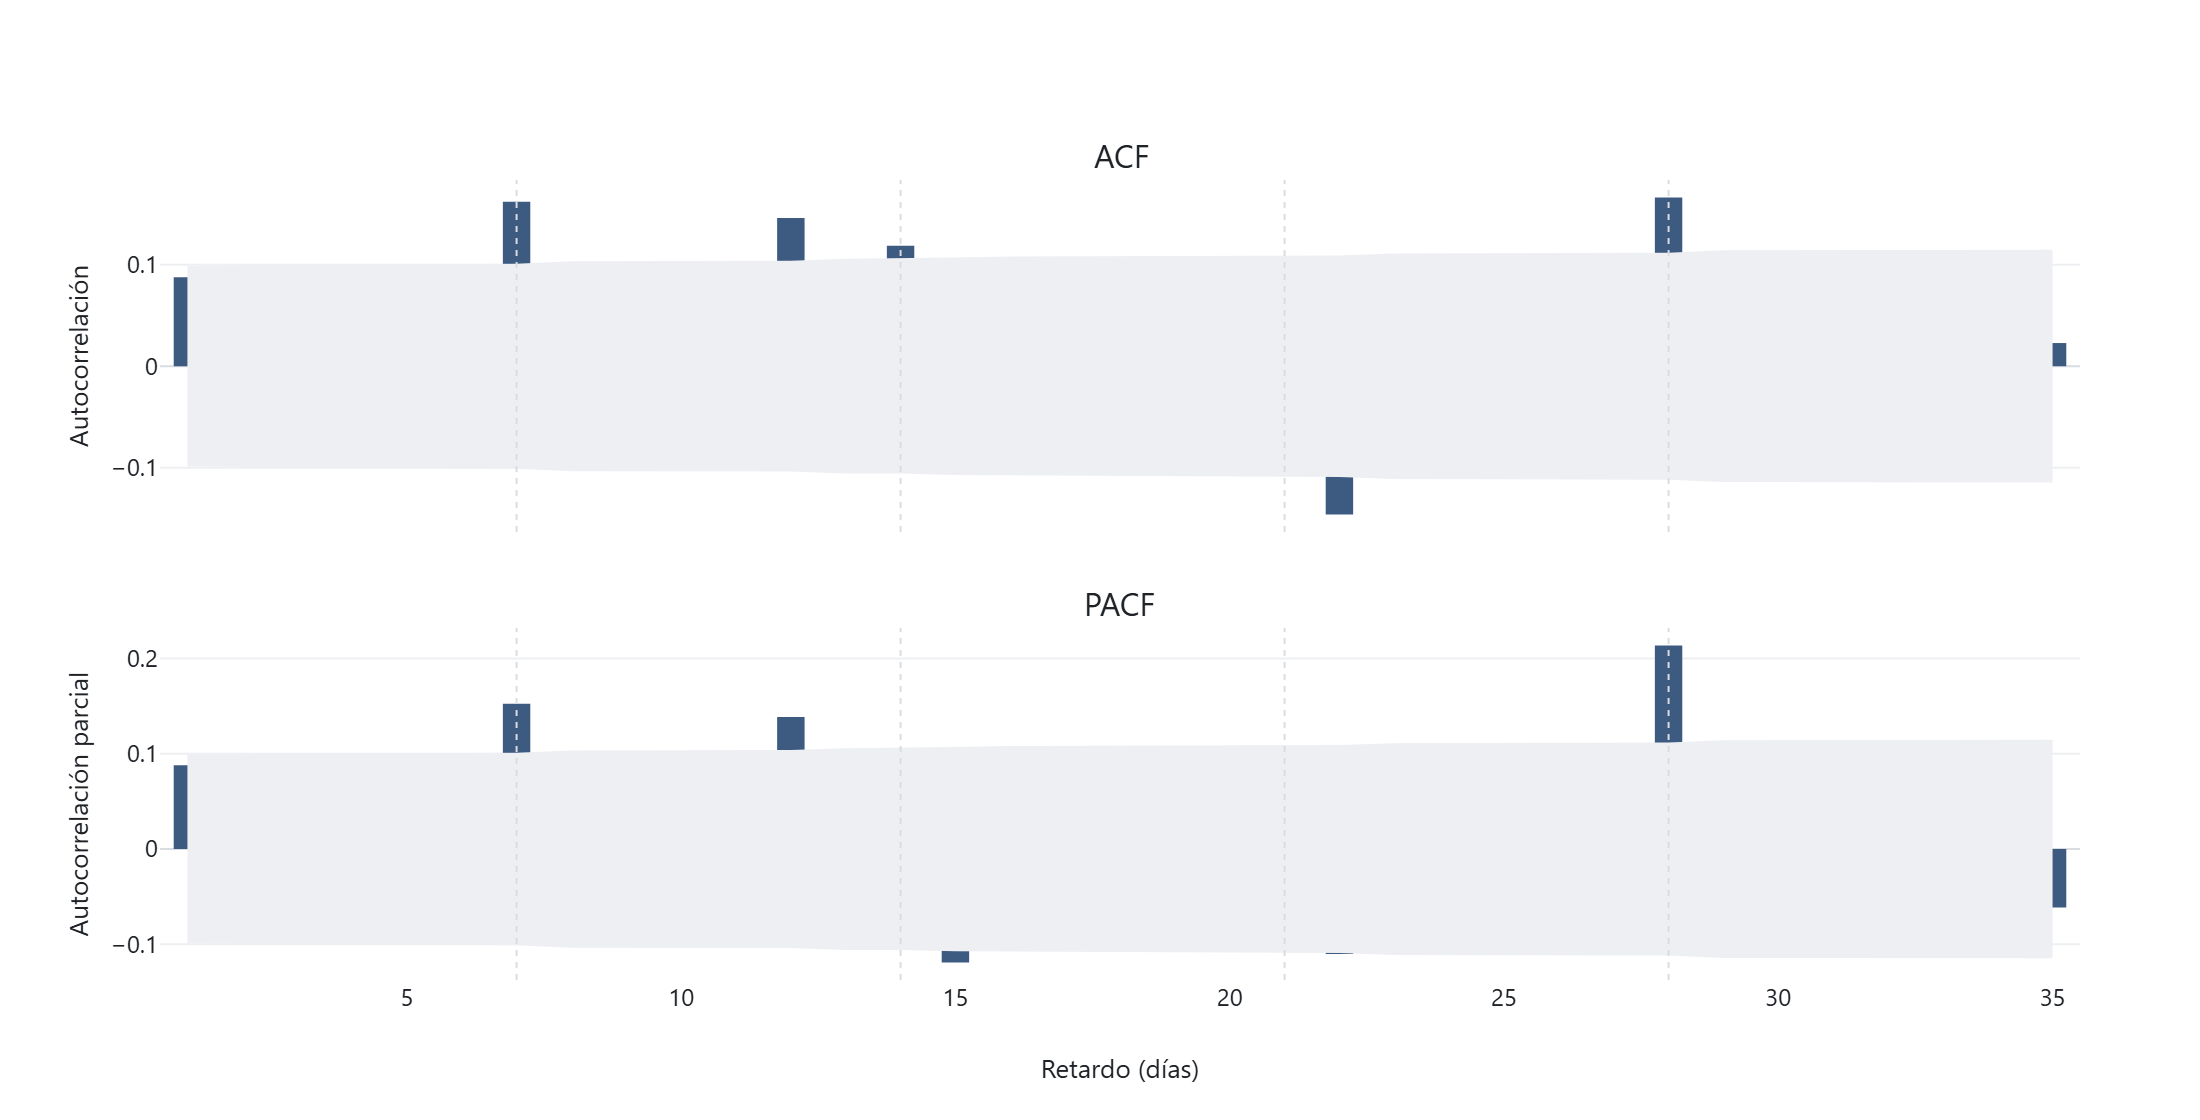
\includegraphics[width=0.78\textwidth]{fig_acf_pacf_residuo_lstm.png}
  \caption{\headlinecolor{ACF y PACF del residuo de la etapa 1 hasta el retardo 35, con la banda de Bartlett sombreada y los retardos semanales (7, 14, 21, 28) marcados. El mayor valor absoluto de la ACF es 0,166 en el retardo 28.}}
  \label{fig:acf_pacf_residuo}
\end{figure}

El periodograma (figura \ref{fig:periodograma_residuo}) matiza esta lectura para la
estacionalidad semanal. La cuota de potencia espectral concentrada exactamente en el intervalo espectral (\emph{bin})
de periodo 7 días es solo 1,4 veces la cuota media, por debajo del factor 3 fijado como
umbral, pero esto se debe en buena medida a la fuga espectral: con 393 observaciones no
existe un \emph{bin} de Fourier exactamente en 7,0 días, y la potencia semanal se reparte entre
los \emph{bins} adyacentes (6,4 y 6,7 días) y, sobre todo, hacia el armónico de 7/3 días, que es
el pico individual más alto de todo el periodograma. La ACF en el retardo 7 (0,162) y, muy
especialmente, el perfil por día de la semana apuntan, por tanto, a una estructura semanal
real que la prueba de \emph{bin} único infravalora.

\begin{figure}[htbp]
  \centering
  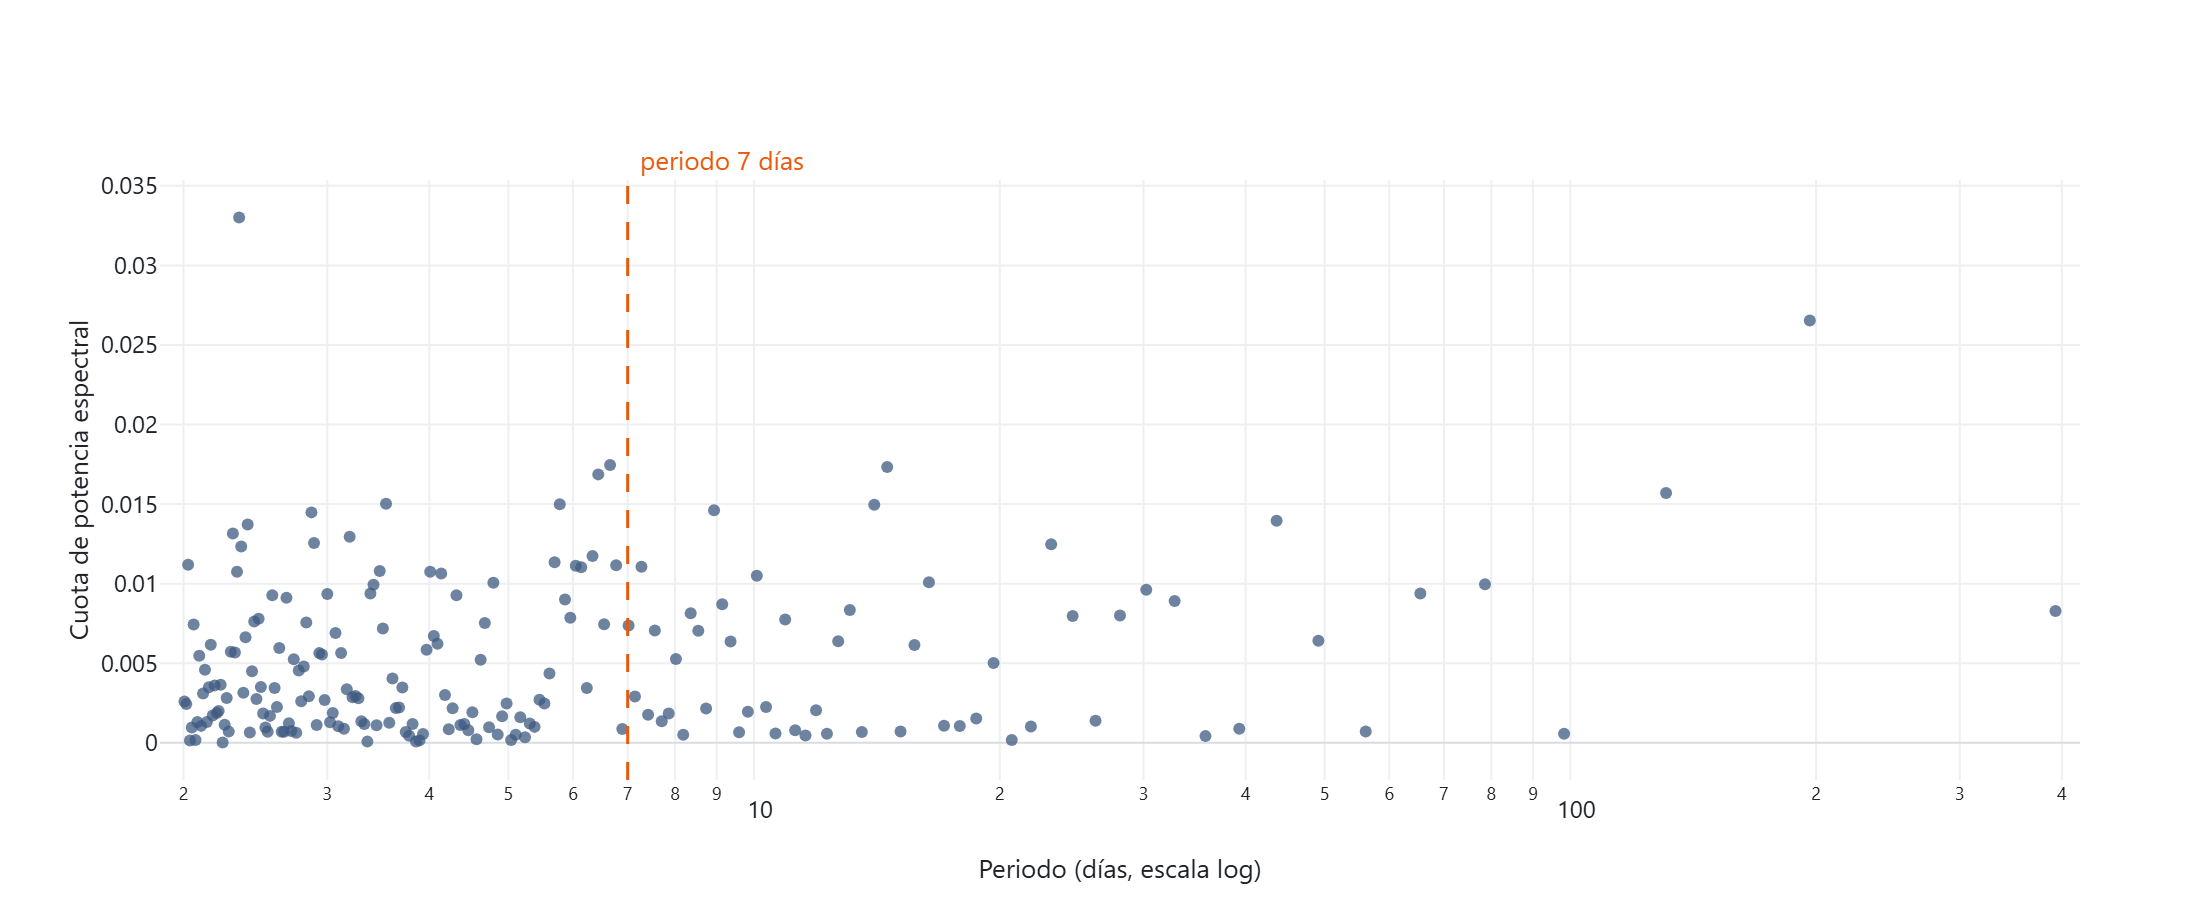
\includegraphics[width=0.78\textwidth]{fig_periodograma_residuo_lstm.png}
  \caption{\headlinecolor{Periodograma del residuo de la etapa 1: cuota de potencia espectral frente al periodo en días (escala logarítmica). El periodo de 7 días está anotado; la potencia semanal se dispersa entre \emph{bins} adyacentes y el armónico de 7/3 días.}}
  \label{fig:periodograma_residuo}
\end{figure}

La tabla \ref{tab:residuo_dia_semana} y la figura \ref{fig:residuo_dia_semana} muestran ese
perfil por día de la semana. La dispersión entre la media de residuo más alta y la más baja
equivale a 0,60 veces la desviación típica del residuo, muy por encima del umbral de 0,30
$\sigma$ para considerar que hay estructura: la etapa 1 sobrepredice sistemáticamente los
sábados (residuo medio $-190.065$, es decir $-0{,}34\,\sigma$) y los jueves ($-0{,}31\,\sigma$),
e infrapredice los lunes y los viernes ($+0{,}26$ y $+0{,}23\,\sigma$). Como la prueba de
significación entre grupos de día viola la independencia (los residuos están
autocorrelacionados), es este tamaño de efecto, y no un valor $p$, el que sostiene la
conclusión de que persiste un sesgo semanal sistemático que la etapa 1 no elimina.

\begin{figure}[htbp]
  \centering
  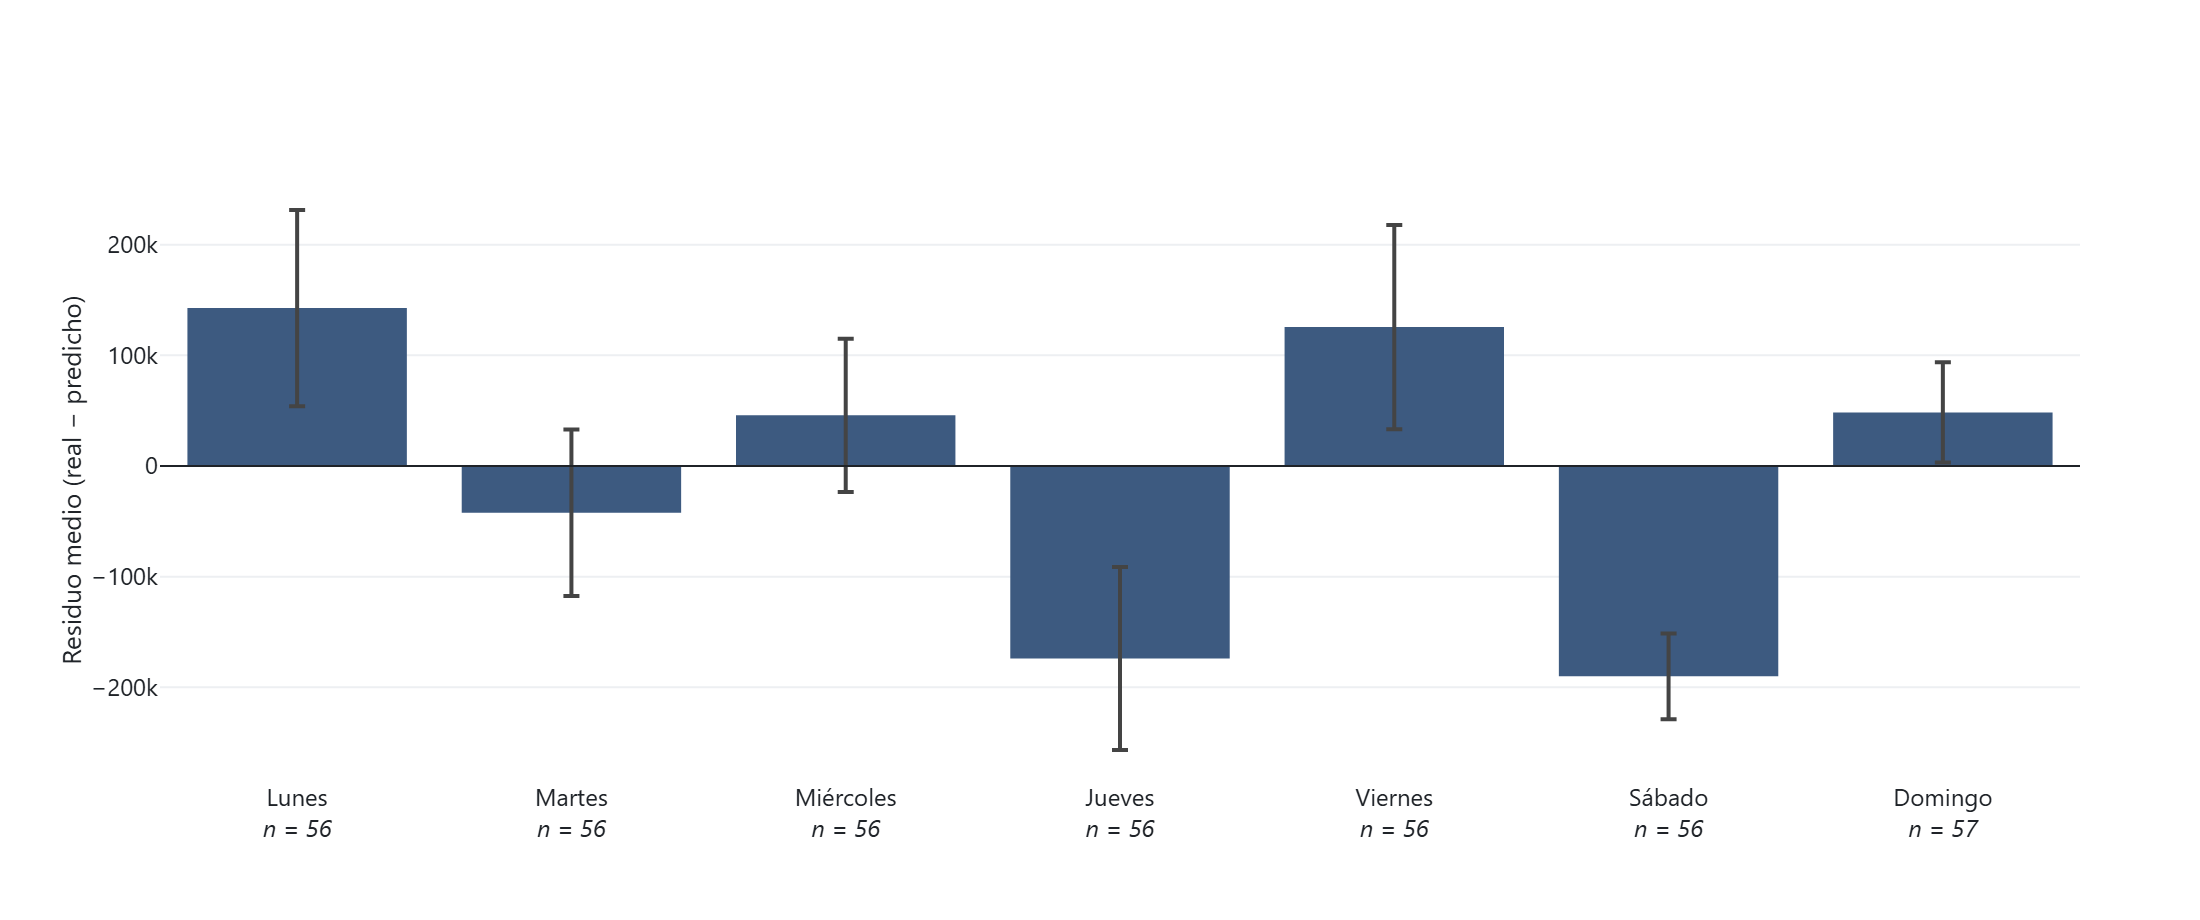
\includegraphics[width=0.78\textwidth]{fig_residuo_por_dia_semana.png}
  \caption{\headlinecolor{Residuo medio de la etapa 1 por día de la semana, con barras de $\pm 1$ error típico y el tamaño muestral bajo cada etiqueta. Una barra positiva indica infrapredicción media de ese día.}}
  \label{fig:residuo_dia_semana}
\end{figure}

Donde el residuo sí retiene estructura con claridad es en el calendario irregular
(tabla \ref{tab:residuo_calendario}). El error absoluto medio de la etapa 1 en los días
festivos, 1.818.580 viajes, es \textbf{6,52 veces} el de los días laborables ordinarios
(279.107), y en los días laborables con puente es 2,96 veces, muy por encima del factor 2
fijado como umbral de concentración. Esta es exactamente la señal que la sección
\ref{sec:importancia_variables} identificó del lado de la etapa 2, donde
\texttt{feat\_day\_type\_festivo} es la variable de mayor ganancia del modelo residual, y
coincide con el diagnóstico exploratorio de la fase 4 sobre el periodo completo. Es también
el único de los cuatro criterios de aceptación prerregistrados que cae con claridad en el
lado de ``la estructura persiste'': la etapa 1 univariante deja sin explicar,
precisamente, la irregularidad de calendario que por construcción no puede ver.

\subsection{Señal meteorológica retardada en el residuo}\label{sec:residuo_meteo_anatomia}

Cabría preguntarse si, además del calendario, el residuo de la etapa 1 retiene señal
meteorológica que la etapa 2 no haya sabido extraer. La tabla \ref{tab:residuo_meteo} y la
figura \ref{fig:residuo_meteo} responden que \textbf{no de forma detectable}. De las 105
variables meteorológicas retardadas (lags de 1, 2, 3 y 7 días y media móvil de 7 días; la
meteorología del mismo día está excluida por diseño y la prueba lo reverifica), ninguna
mantiene una correlación de Spearman \emph{parcial} estadísticamente significativa con el
residuo tras controlar por los cuatro términos anuales de Fourier y aplicar la corrección
de Benjamini-Hochberg al 10\,\%. La brecha entre la correlación bruta y la parcial es,
en sí misma, el hallazgo: la humedad relativa máxima retardada un día y la temperatura
máxima retardada dos días presentan correlaciones brutas de $0{,}28$ en valor absoluto,
pero al partializar por el ciclo anual, que ambas comparten con la demanda, colapsan a
$0{,}11$ y $0{,}09$, y no sobreviven a la corrección por comparaciones múltiples.

La lectura correcta de este resultado nulo, a la luz de la objeción metodológica registrada
para esta fase, no es que la arquitectura híbrida debiera haber funcionado: la etapa 2
\emph{recibió} esas 105 variables —de hecho, la sección \ref{sec:importancia_variables}
mostró que la meteorología retardada concentra el 51,6\,\% de su ganancia— y aun así el
híbrido pierde. Lo que este análisis indica es que no se observa señal meteorológica
retardada sin explotar en el residuo; lo que el residuo retiene es estructura de calendario,
no de clima. Que un bloque de variables acapare la mitad de la ganancia por impureza y a
la vez no mantenga ninguna correlación parcial detectable con el residuo es solo
aparentemente contradictorio; la sección \ref{sec:lectura_conjunta} reconcilia ambos
hechos con el tercero que aporta la fase siguiente, la ablación del bloque completo.

\begin{figure}[htbp]
  \centering
  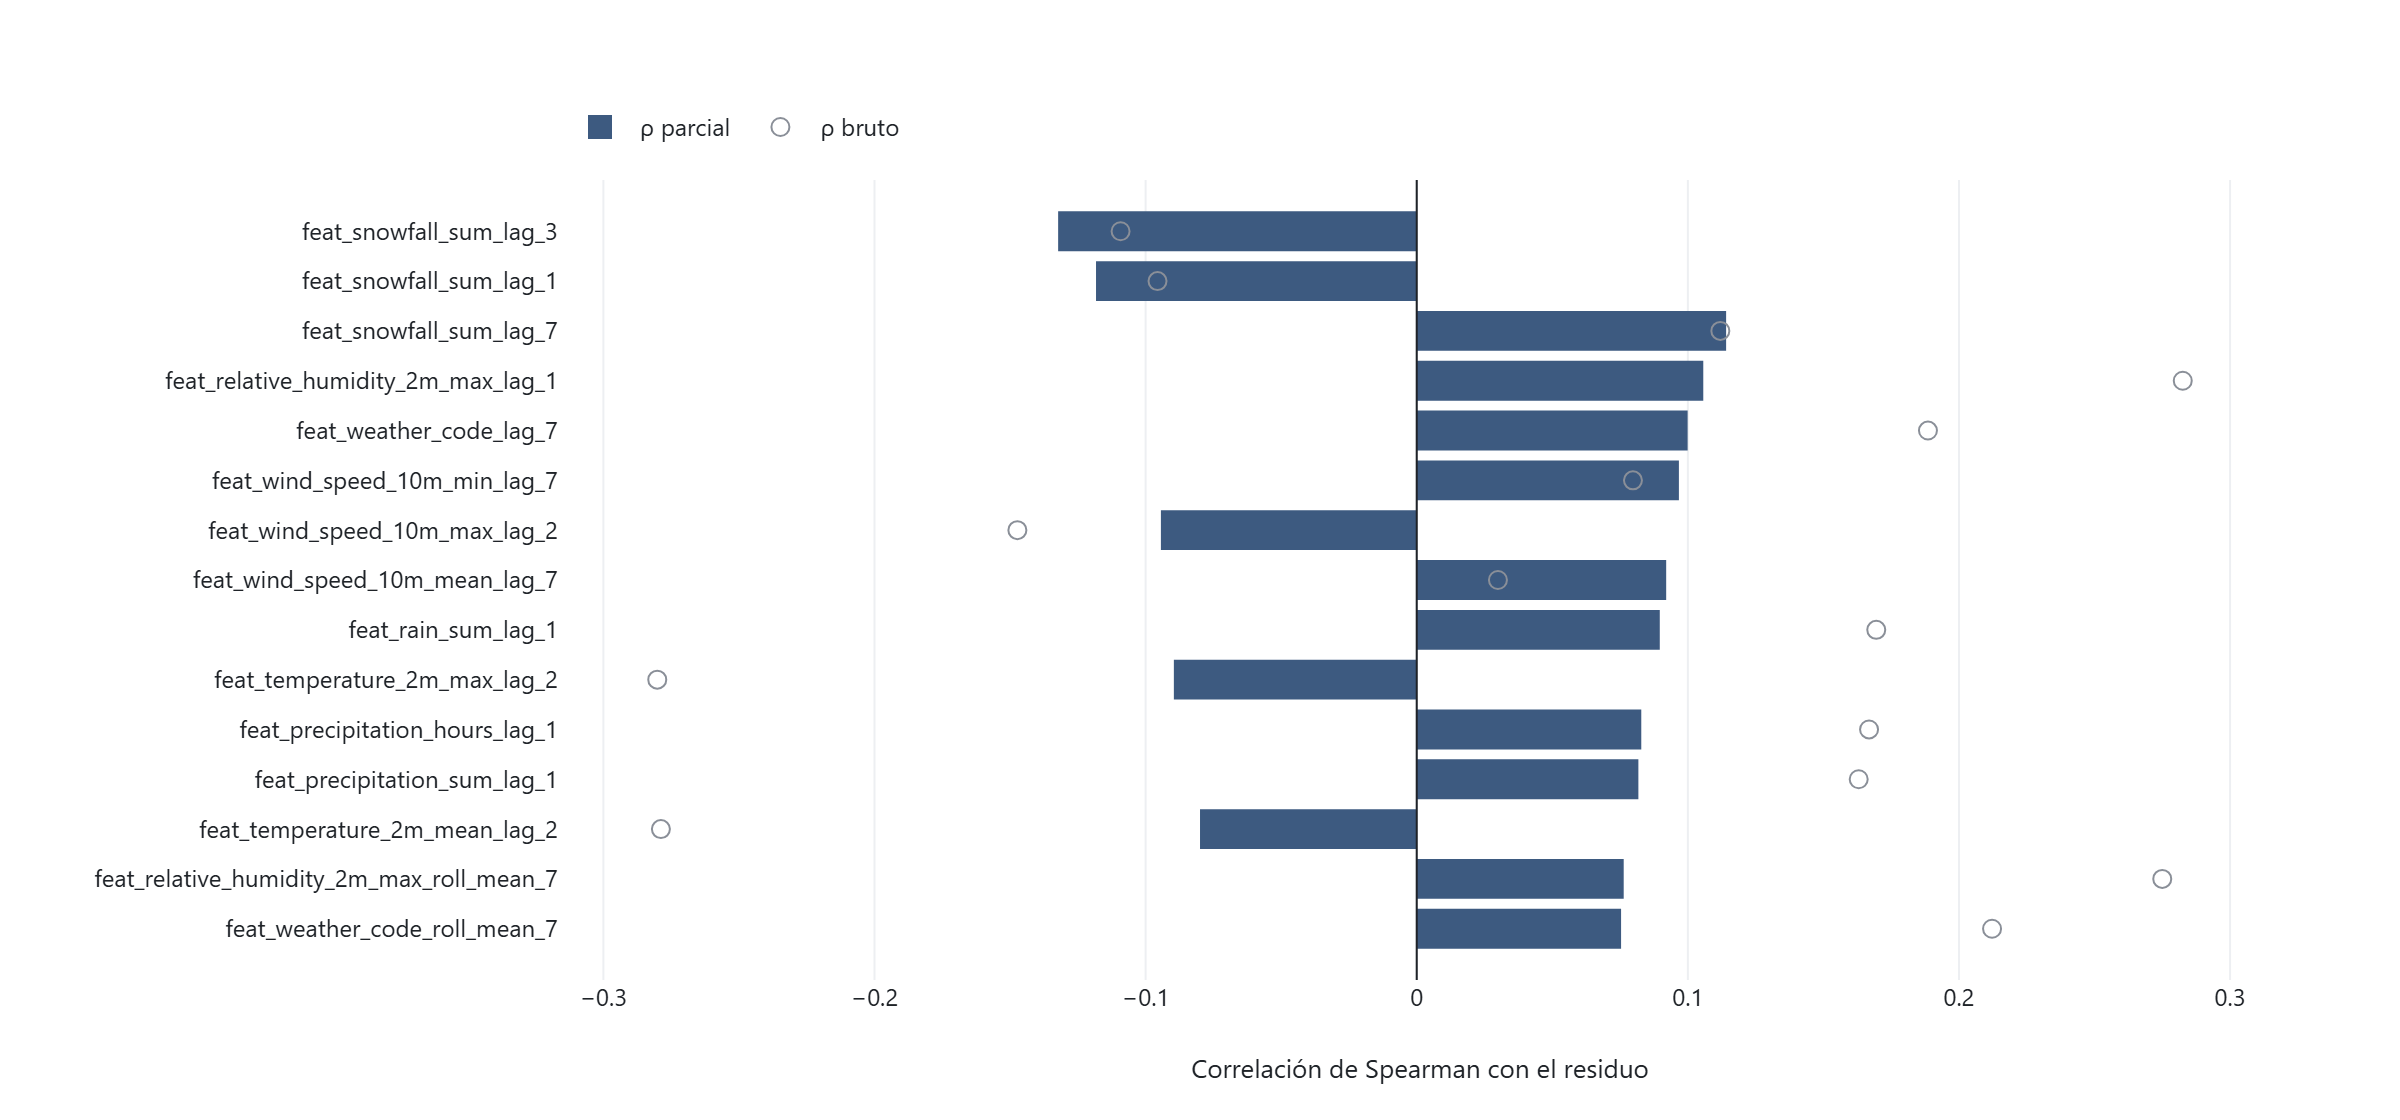
\includegraphics[width=0.78\textwidth]{fig_residuo_vs_meteo.png}
  \caption{\headlinecolor{Correlación de Spearman del residuo de la etapa 1 con las 15 variables meteorológicas retardadas de mayor $|\rho$ parcial$|$. El marcador hueco muestra la $\rho$ bruta: la distancia entre ambos es el efecto del ciclo anual compartido.}}
  \label{fig:residuo_meteo}
\end{figure}

\subsection{La cadena de error, cuantificada}\label{sec:cadena_error}

La tabla \ref{tab:cadena_error} y la figura \ref{fig:cadena_error} cuantifican cuánto de la
distancia entre una LSTM univariante y un XGBoost independiente cierra realmente la etapa
residual. No es una descomposición (\texttt{lstm\_alone}, \texttt{hybrid} y
\texttt{xgboost\_alone} son tres modelos distintos, no sumandos de un mismo error), sino
una cadena de tres puntos evaluados con el mismo \texttt{metrics.all\_metrics} que la tabla
maestra, de modo que no puede contradecirla. Sobre la partición test, la distancia
completa entre \texttt{lstm\_alone} (MAE 280.952) y \texttt{xgboost\_alone} (156.121) es de
124.831 viajes diarios. La etapa 2 recorta 46.729 de esa distancia, el \textbf{37,4\,\%}
del hueco, dejando todavía 78.103 (el 62,6\,\%) de separación entre el híbrido corregido y
un XGBoost independiente sobre las mismas 161 variables. Sobre validación la corrección es
proporcionalmente mucho mayor (130.405, el 78,4\,\% de un hueco más ancho porque
\texttt{lstm\_alone} rinde bastante peor en esa partición), pero los 35.895 viajes
restantes siguen favoreciendo a \texttt{xgboost\_alone}. La conclusión es la misma en ambas
particiones y coincide con lo anticipado en la sección \ref{sec:contraste_central}: la
etapa residual es una corrección real y sustancial, pero parte de tan atrás que la
corrección, por grande que sea, no alcanza a un modelo de una sola etapa.

\begin{figure}[htbp]
  \centering
  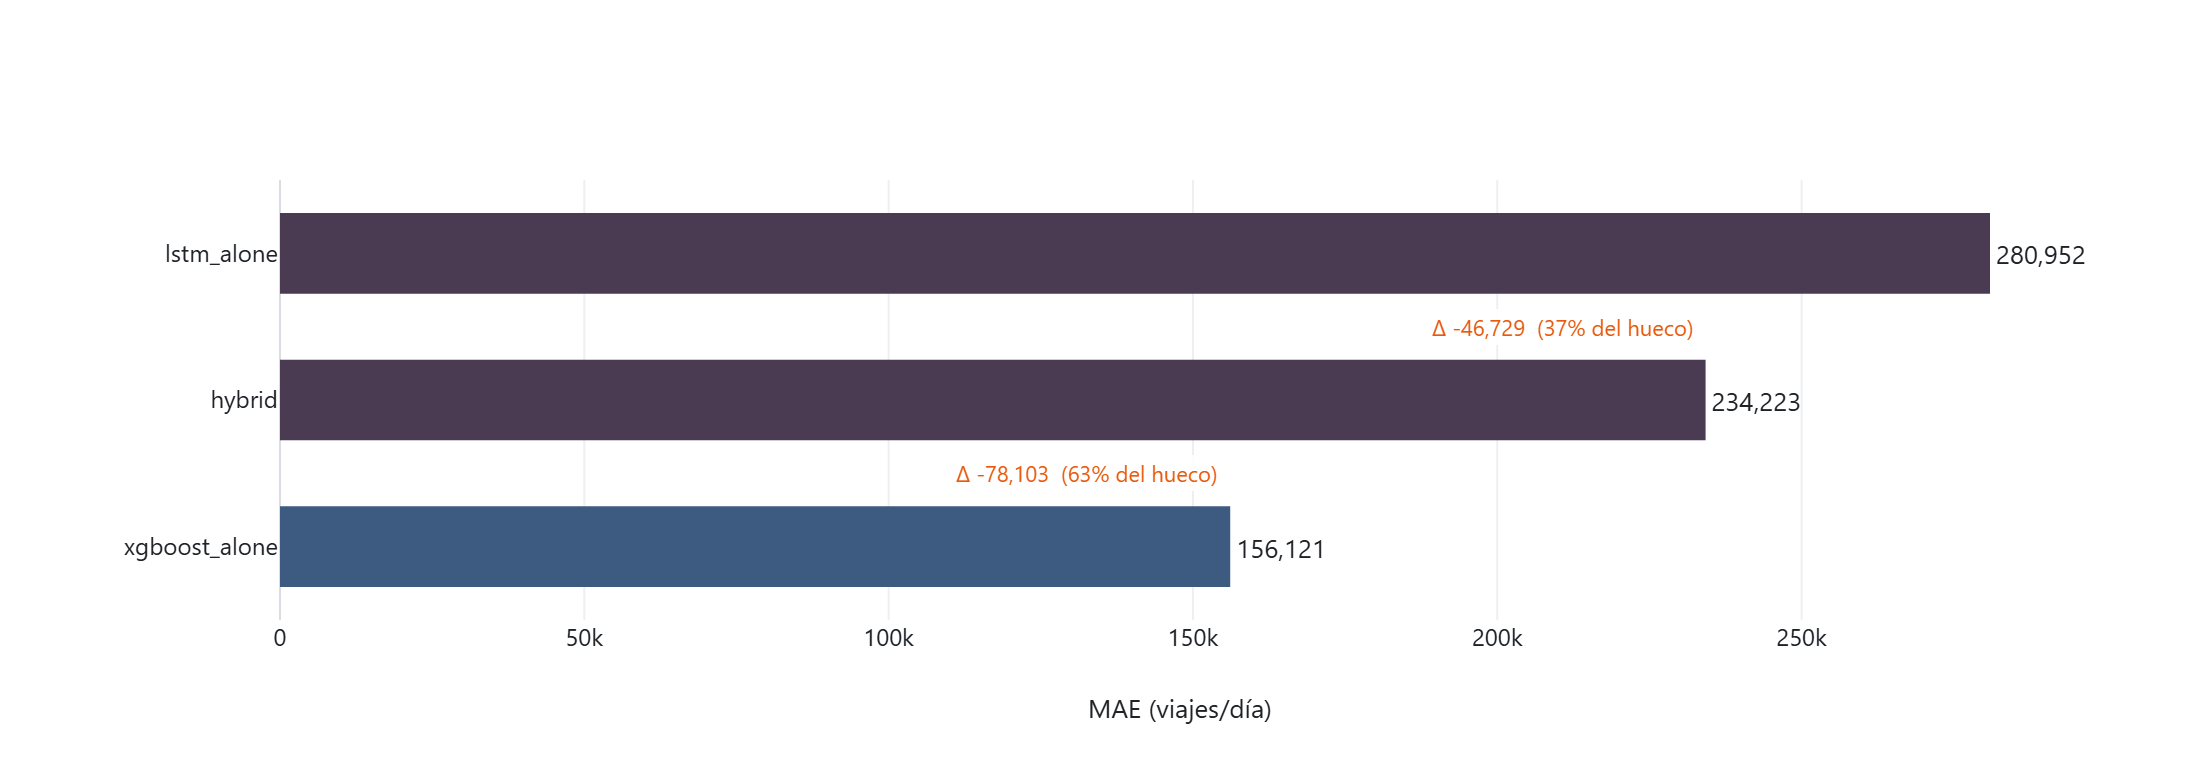
\includegraphics[width=0.78\textwidth]{fig_cadena_error.png}
  \caption{\headlinecolor{Barras escalonadas del MAE de test de los tres modelos de la cadena, con el paso entre barras consecutivas anotado en MAE absoluto y como cuota del hueco total. Deliberadamente no es una cascada con conectores.}}
  \label{fig:cadena_error}
\end{figure}

\subsection{Contexto de tamaño muestral}\label{sec:tamano_muestral}

Queda por sustentar con evidencia la afirmación de que la debilidad de la etapa 1 es, en
lo esencial, un problema de tamaño de muestra. Un primer indicio, solo un indicio, procede
de los cinco folds de validación \emph{out-of-fold}. El
MAE por fold no decrece de forma monótona al crecer el tamaño de entrenamiento: cae de
1.461.905 (fold 1, 200 filas) a 282.122 (fold 3, 474 filas) y vuelve a subir a unos
500.000 en los folds 4 y 5, porque cada fold predice además un periodo distinto y de
dificultad distinta. Expresar el error de cada fold como \emph{ratio de habilidad} frente a
\texttt{seasonal\_naive} evaluado sobre exactamente el mismo bloque de fechas atenúa en
parte ese factor de confusión: los folds 3 y 5 alcanzan la paridad con el baseline
estacional (ratios de 0,95 y 0,98), el fold 1 permanece degenerado (2,67) y los folds 2 y
4 quedan por encima de 1. Con cinco puntos, no monótonos y confundidos con la dificultad
del periodo evaluado, esto es contexto indicativo y no una curva de aprendizaje.

La evidencia principal sobre el papel del tamaño de muestra procede de una curva de
aprendizaje propiamente dicha (tabla \ref{tab:curva_aprendizaje} y figura
\ref{fig:curva_aprendizaje}), el único experimento de esta fase que reentrena. Se ajusta
una LSTM de etapa 1, con la arquitectura de la fase 4, sobre ventanas de entrenamiento de
tamaño creciente, en seis fracciones del bloque de entrenamiento post-calentamiento (de
222 a 889 filas), con tres semillas por fracción para poder leer la mediana y la banda
mín-máx en lugar de una única ejecución ruidosa. El conjunto de evaluación se mantiene
fijo (siempre la partición de validación completa) y la partición de test no se consulta
en ningún momento. La ventana de entrenamiento es \textbf{descendente}, anclada en
\texttt{train\_end} y creciendo hacia atrás: esta elección es deliberadamente
conservadora para un experimento de tamaño de muestra, porque las fracciones más pequeñas
entrenan sobre las filas temporalmente más próximas a validación y disfrutan, por tanto, de
una ventaja de recencia; el diseño está sesgado \emph{en contra} de encontrar un efecto de
tamaño de muestra, de modo que un efecto que sobreviva a ese sesgo es más creíble y un
resultado plano es correspondientemente más débil de lo que parecería a primera vista.

El resultado es una historia de tamaño de muestra \textbf{parcial}, y se reporta como tal.
Por un lado, el tamaño de
muestra importa, y mucho, en el extremo bajo: con 222 filas de entrenamiento el modelo
\textbf{colapsa} (las tres semillas producen ajustes degenerados, con un cociente de
desviaciones típicas entre 0,30 y 0,43 y una correlación con la serie real en torno a
0,45, es decir, predicciones cuasi-constantes), exactamente el mismo modo de fallo
documentado para el fold 1 en la sección \ref{sec:esquema_oof}. Pasar de 222 a 356 filas
reduce el MAE de validación mediano de 1.167.187 a 515.603, y a partir de ahí el descenso
continúa, pero se aplana: 502.449 con 489 filas, 490.773 con 622, y ya prácticamente estable
en torno a 411.000-416.000 con 756 y 889 filas, dentro del ruido entre semillas.

Por otro lado, y esto es lo que la curva sí muestra, esa meseta se sitúa muy por encima de ambas
referencias de una sola etapa: el mejor punto LSTM de toda la curva, unos 411.000 de MAE de
validación, sigue estando aproximadamente 166.000 viajes por encima de
\texttt{xgboost\_alone} (244.843) y 138.000 por encima de SARIMAX (273.467), y las tres
fracciones superiores no muestran ninguna tendencia a acercarse a esas líneas. La lectura
correcta, por tanto, no es que ``con más datos la vía LSTM ganaría'': el tamaño de muestra
explica por qué la etapa 1 es \emph{muy} débil en lugar de solo débil —el colapso por
debajo de unas 350 filas y la fuerte ganancia inicial son reales—, pero el techo de una
arquitectura univariante sobre esta serie se encuentra, incluso con todos los datos
disponibles y bajo un diseño de ventana que la favorece, claramente por encima de los
modelos de una sola etapa a los que el híbrido aspira a superar.

\begin{figure}[htbp]
  \centering
  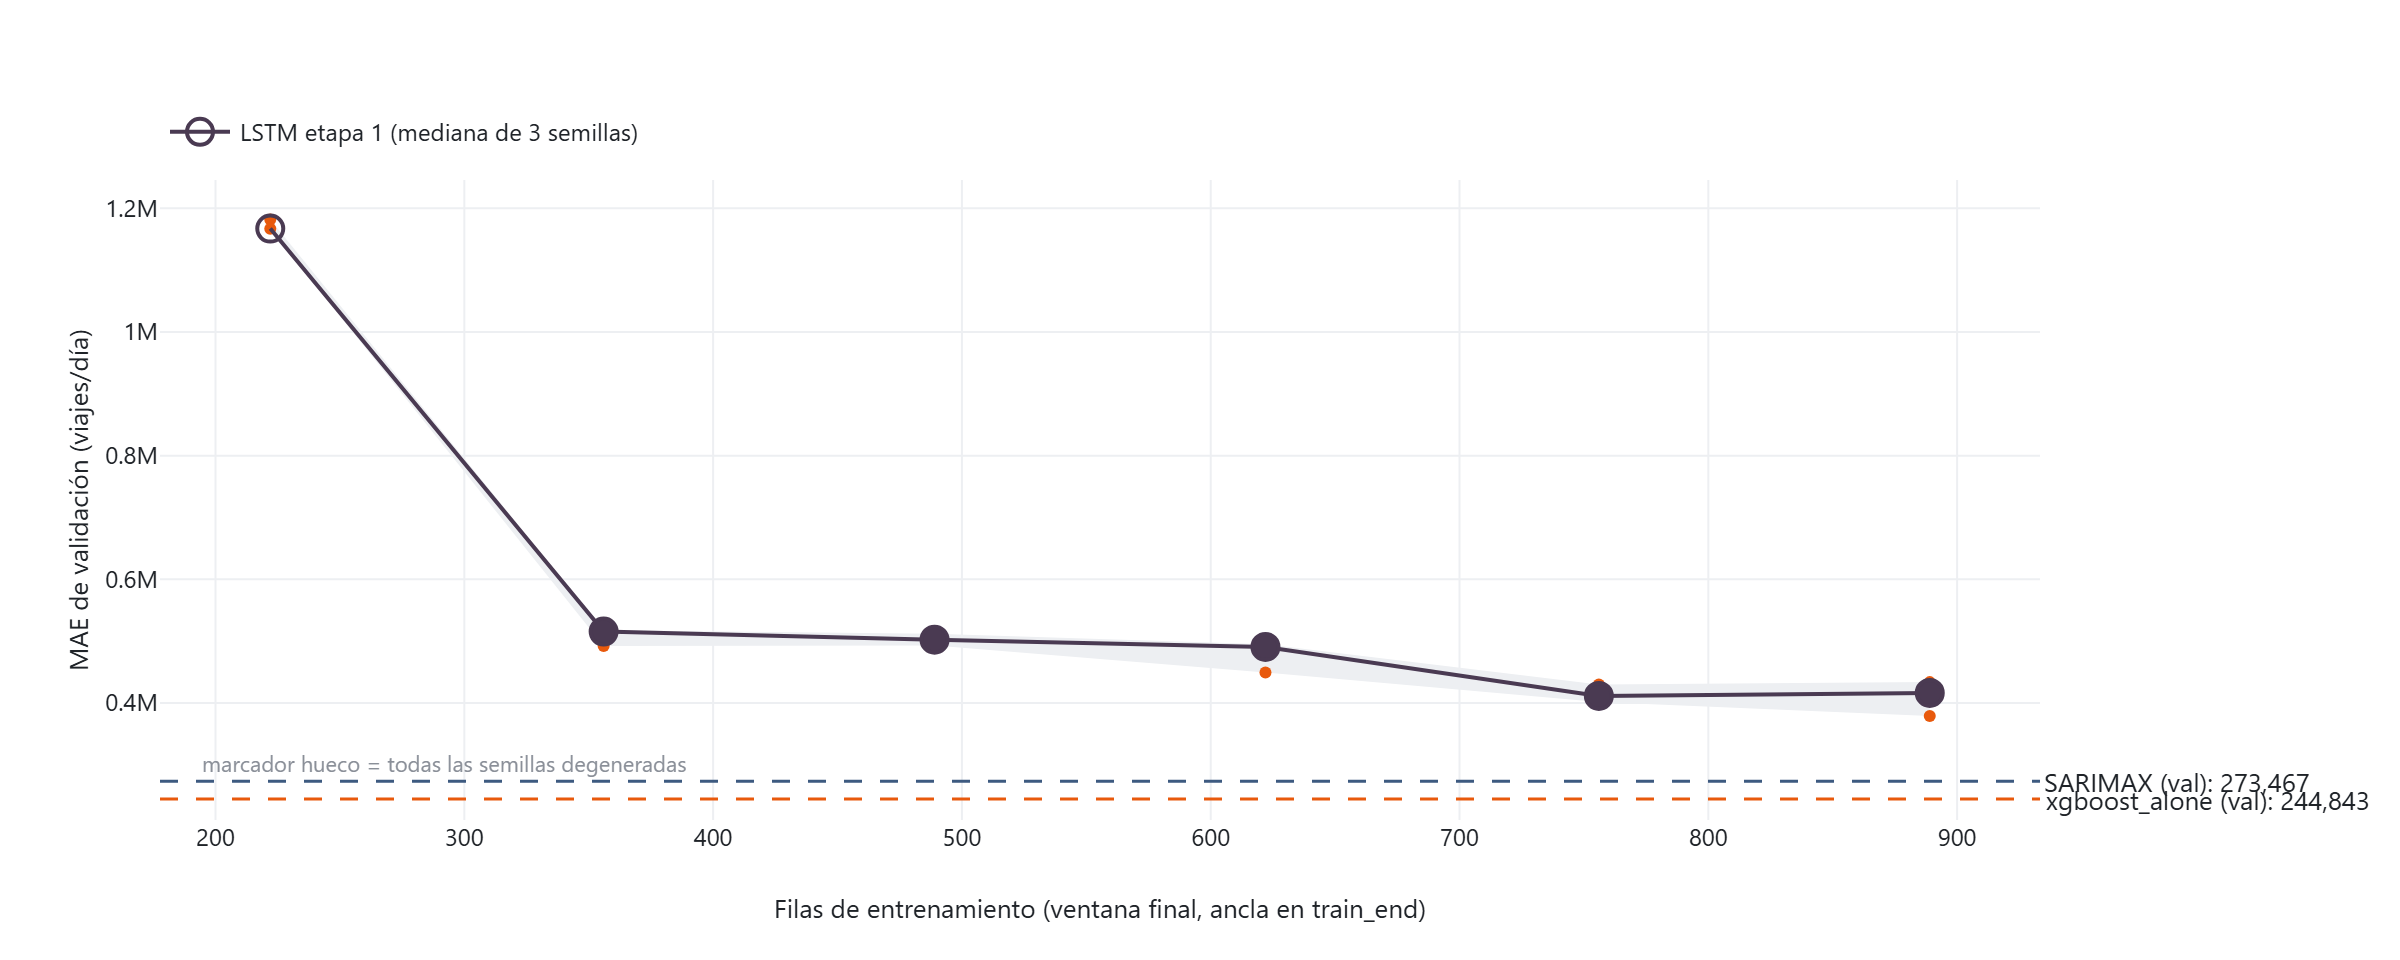
\includegraphics[width=0.78\textwidth]{fig_curva_aprendizaje_lstm.png}
  \caption{\headlinecolor{MAE de validación de la LSTM de etapa 1 frente a las filas de entrenamiento (ventana descendente anclada en \texttt{train\_end}): mediana y banda mín-máx de 3 semillas (5 en la fracción 1,00), con las líneas de referencia de SARIMAX y \texttt{xgboost\_alone} en validación. El marcador hueco indica la fracción cuyas tres semillas degeneraron. La curva se aplana muy por encima de ambas referencias.}}
  \label{fig:curva_aprendizaje}
\end{figure}

\section{Paridad informativa entre etapas: ablación y control LSTM}\label{sec:paridad_informativa}

La sección \ref{sec:anatomia_residuo_etapa1} midió \emph{qué} retiene el residuo de la
etapa 1; esta sección se pregunta algo distinto: si la partición del problema en dos etapas
está \emph{informativamente} justificada. El análisis anterior deja dos cuestiones
abiertas. La primera (Q1): la etapa 1 es univariante mientras que
XGBoost ve 161 variables desde el principio, así que ambas etapas no son equivalentes en
información; ¿pierde la etapa 1 por ser una \emph{LSTM} o por ser \emph{univariante}? La
segunda (Q2): ¿integra ya el XGBoost independiente los efectos temporales y exógenos de forma
simultánea a través de las variables construidas, de modo que separar el problema en dos
etapas añade complejidad sin añadir información predictiva? Esta sección deja de conjeturar
y lo mide con dos controles. Como la sección \ref{sec:anatomia_residuo_etapa1}, es un
análisis \textbf{confirmatorio} y un control diagnóstico bajo el régimen ya declarado allí;
sus dos controles sí reentrenan, pero no persisten ningún artefacto bajo \texttt{models/}.

\subsection{Ablación de bloques de variables sobre \texttt{xgboost\_alone}}\label{sec:ablacion_bloques}

Se reentrena \texttt{xgboost\_alone} sobre subconjuntos restringidos de variables,
manteniendo idénticos la partición de entrenamiento (889 filas tras el descarte de
calentamiento), la rejilla de 54 puntos, el \emph{holdout} cronológico interno y el
protocolo de evaluación; lo único que cambia es qué bloques son visibles. Los subconjuntos
—\texttt{completo} (161 variables), \texttt{solo\_temporal} (39: retardos de \texttt{total}
y de operadores más medias móviles), \texttt{solo\_exogeno} (122: calendario, Fourier y
meteorología), \texttt{sin\_meteo} (56) y \texttt{solo\_calendario} (17)— se fijaron
\emph{antes} de ver ningún resultado, y el criterio de materialidad (un bloque aporta si
retirarlo eleva el MAE de validación en al menos un 5\,\% respecto a \texttt{completo}) es
una constante de módulo evaluada en código, no mediante inspección manual. El umbral del 5\,\% absorbe el ruido
de rejilla y semilla, ya que cada subconjunto rehace su propia búsqueda de
hiperparámetros.

Esto es un \textbf{estudio de retirada de bloques, no una descomposición}. Los bloques
\textbf{no son disjuntos en información}: \texttt{fourier\_annual} y la meteorología
retardada codifican ambos el ciclo anual —la sección \ref{sec:residuo_meteo_anatomia} lo
midió, viendo colapsar las correlaciones al parcializar por los términos anuales—, y los
retardos 7/14/21/28 de \texttt{total} codifican implícitamente el calendario semanal. Por
tanto, \texttt{solo\_temporal} sigue ``sabiendo'' el día de la semana y \texttt{solo\_exogeno}
sigue ``sabiendo'' la estación. Las columnas de la tabla \ref{tab:ablacion_bloques} no
suman a nada y no deben leerse como contribuciones aditivas.

El resultado responde a Q2 de la forma prevista: \textbf{\texttt{solo\_temporal} y
\texttt{solo\_exogeno} empeoran ambos por encima del umbral}, un 88,6\,\% y un 30,9\,\% de
MAE de validación respectivamente, de modo que el modelo de una sola etapa
\textbf{integra internamente los dos tipos de información}. Esto es la corroboración
mecánica del resultado ya establecido en la sección \ref{sec:contraste_central} (no una
prueba nueva; el capítulo ya mostró la mitad predictiva, que el híbrido pierde): la
división en dos etapas hace, a través de etapas, lo que un único modelo tabular ya hace en
una. Dos lecturas secundarias, reportadas sin veredicto de aprobado/suspenso:
\texttt{solo\_calendario} (17 variables) queda un 22,8\,\% por encima de \texttt{completo}
, sustancial pero lejos de la paridad, así que la serie no está determinada solo por el
calendario determinista; y \texttt{sin\_meteo} rinde un 3,2\,\% \emph{mejor} que
\texttt{completo}, es decir, el bloque de 105 columnas meteorológicas no se gana su sitio y
actúa como ruido neto leve, en línea con el hallazgo de la sección
\ref{sec:residuo_meteo_anatomia} de que la meteorología retardada es cuasi-ruido-blanco en
el residuo. La figura \ref{fig:ablacion_bloques} ordena los cinco subconjuntos por MAE de
validación y superpone el MAE de test de cada uno, de modo que el orden de la ablación
pueda leerse directamente junto con su estabilidad entre particiones.

\begin{figure}[htbp]
  \centering
  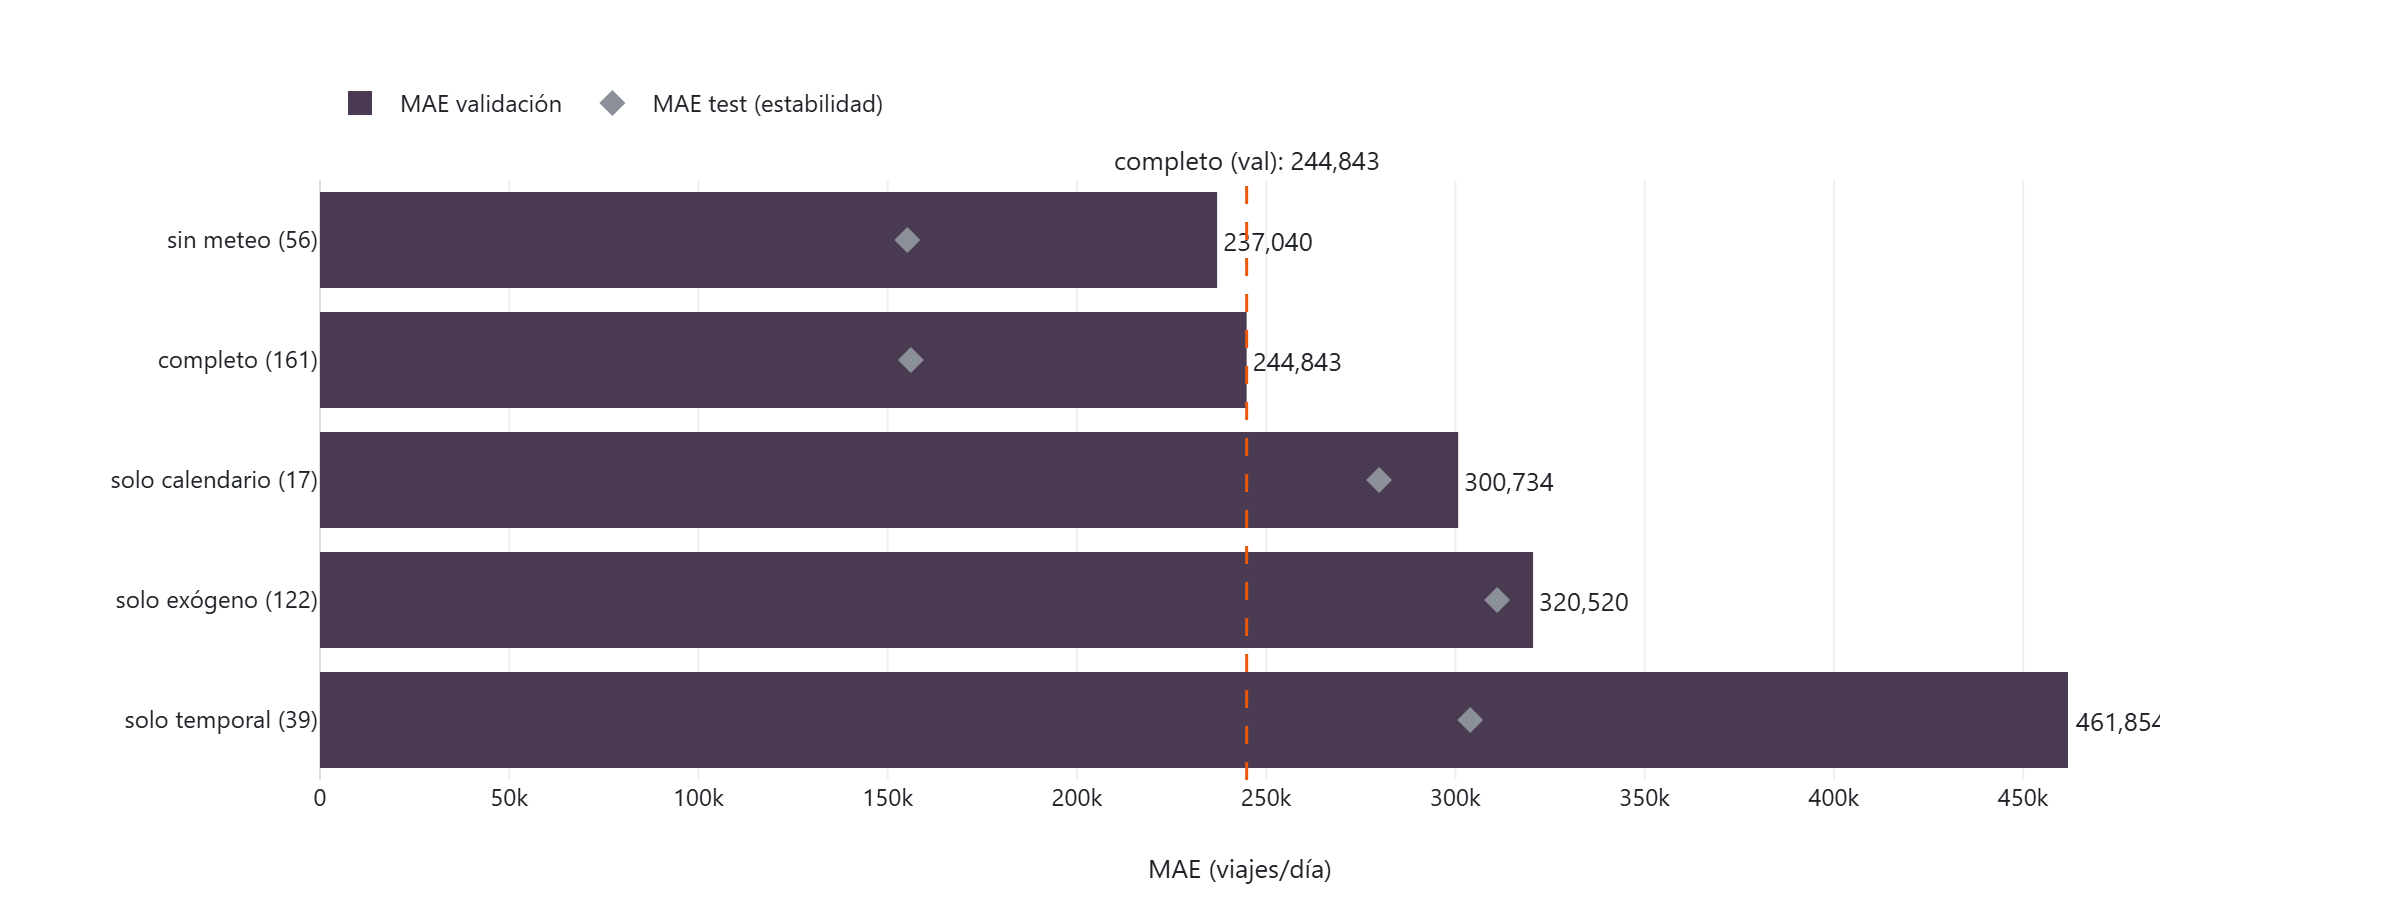
\includegraphics[width=0.78\textwidth]{fig_ablacion_bloques.png}
  \caption{\headlinecolor{MAE de \texttt{xgboost\_alone} reentrenado sobre subconjuntos restringidos de variables, mejor subconjunto arriba. La línea discontinua marca el MAE de validación de \texttt{completo} (244.843) y los rombos el MAE de test como comprobación de estabilidad. Retirar el bloque temporal o el exógeno empeora el modelo por encima del umbral del 5\,\%; retirar la meteorología no.}}
  \label{fig:ablacion_bloques}
\end{figure}

\subsection{LSTM en paridad informativa}\label{sec:paridad_lstm}

Para responder a Q1 se dota a la rama recurrente de \textbf{paridad informativa}: la ventana
de 28 pasos del objetivo alimenta la LSTM y el vector de variables predictoras \texttt{feat\_}
del \emph{propio día $t$} se concatena después
(\texttt{Input}$(W,1)\to$\texttt{LSTM}$\to$\texttt{concat}(\texttt{Input}$(k)$)$\to$
\texttt{Dropout}$\to$\texttt{Dense}$(1)$). Es el cambio mínimo que logra paridad real: una
ventana multivariante $(W,k)$ daría el calendario de los 28 días previos, pero no el del día
que se predice, porque la ventana abarca $[t-W, t)$ y excluye la fila $t$ por construcción.
Cada columna es la misma fila, sujeta a las mismas guardias anti-fuga, que ve XGBoost
(guardas de las fases 2 y 3: sin operadores del mismo día, sin meteorología del mismo
día), y una aserción
reverifica el prefijo \texttt{feat\_} en el punto de entrada.

La interpretación es asimétrica y se declara antes de los resultados (objeción O4):
la LSTM en paridad ve una ventana cruda de 28 pasos \emph{más} el vector del día $t$, es
decir, estrictamente \emph{más} información que el vector plano de XGBoost (que solo dispone
de 7 retardos seleccionados y 4 estadísticos móviles). En consecuencia, \textbf{una derrota
clara sería una conclusión fuerte} (la asimetría informativa quedaría descartada como causa
dominante) y \textbf{una victoria es débil} (procede en parte de información extra, no solo
de la arquitectura). Y un buen resultado aquí sería un argumento \emph{contra} el híbrido,
no a favor de uno mejor: una etapa 1 que ya ve la matriz de la etapa 2 no deja a esta nada
que corregir que la etapa 1 no pudiera ver.

\textbf{Base de comparación y número de semillas.} El punto de referencia es la LSTM
univariante de la fase 4. Se compara contra su mediana de cinco semillas
(42, 1, 2, 3, 4) en la fracción 1,00 de la curva de aprendizaje de la sección
\ref{sec:tamano_muestral}, \textbf{416.324} de MAE de validación, y no contra su mejor
semilla individual (411.142; cuadro \ref{tab:paridad_lstm}). El veredicto de paridad se lee sobre una mediana de
cinco semillas, así que la base tiene que ser también una mediana de cinco semillas (mismo
arnés, mismas semillas, misma partición de validación, genuinamente comparable); enfrentar
una mediana contra un mejor caso sesgaría el cierre del hueco a la baja, hacia la
conclusión que el TFM ya defiende, que es justo donde el análisis debe ser más estricto. La
mediana de cinco semillas resulta coincidir con la de tres (la semilla 1 es el valor
central en ambos casos), de modo que el hueco a cerrar sigue siendo $416.324 - 244.843 =
171.481$ y los umbrales no cambian.

El paso de tres a cinco semillas se decidió por la
regla prerregistrada (secciones de método y objeción O6: subir a cinco solo si la sonda de
tiempos muestra holgura, decidido \emph{antes} de la ejecución); la sonda mostró amplia
holgura (el ajuste más lento fue de 9,7\,s frente a un techo de unos 6\,min). La sonda
también dejó visibles unos MAE de validación provisionales con semilla 42 (395.274 en
\texttt{calendario}, 369.835 en \texttt{completo}), ambos dentro de la banda ambigua del
25--60\,\%; se hace constar explícitamente que esas cifras \emph{eran} visibles antes de
elegir el número de semillas y que la regla, basada en holgura de cómputo, gobierna con
independencia de dónde cayeran.

\textbf{Lecturas prerregistradas.} Con un hueco de 171.481, cerrar el $\geq$ 60\,\%
(MAE de validación mediano $\leq 313.435$) se lee como \emph{asimetría informativa}: la
debilidad de la etapa 1 está dominada por lo que no se le dejó ver. Cerrar el $\leq$ 25\,\%
(mediano $\geq 373.454$) se lee como \emph{limitación arquitectónica}: un modelo
recurrente simplemente no es competitivo en este problema a este tamaño de muestra, ni
siquiera en paridad informativa. Entre ambos, \emph{mixto/ambiguo}. La degeneración se
evalúa primero: si la mayoría de semillas de un ámbito degenera, el veredicto es
\emph{fallo de capacidad/muestra}. Y si la banda mín-máx cruza un umbral, el veredicto se
degrada a \emph{mixto/ambiguo} con independencia de dónde caiga la mediana (objeción O6).

\textbf{Resultado.} Ninguno de los dos ámbitos se acerca a cerrar el hueco (tabla
\ref{tab:paridad_lstm}, figura \ref{fig:paridad_lstm}). Ninguna semilla degenera y ninguna
queda infra-entrenada (\texttt{best\_epoch} mediano 75 y 53, muy por encima del umbral de
20). El ámbito \texttt{calendario} ($k=17$), el más nítido para la afirmación de ceguera al
calendario, cierra solo un \textbf{16,2\,\%} del hueco (MAE de validación mediano 388.625;
banda 382.695--395.877, sin cruce de umbral): veredicto \emph{limitación
arquitectónica}. Es decir, dada exactamente la información de calendario y Fourier donde la
sección \ref{sec:residuo_estructura} localizó la estructura del residuo, un modelo
recurrente en paridad informativa apenas recupera una sexta parte de la distancia hasta
XGBoost. El ámbito \texttt{completo} ($k=161$) lo hace mejor, cierra un \textbf{31,0\,\%}
(mediano 363.133), pero su banda (354.235--391.630) cruza el umbral del 25\,\%, de modo que
el veredicto se degrada a \emph{mixto/ambiguo}; y por la asimetría O4 un cierre parcial es
de todos modos evidencia débil. En conjunto, la respuesta a Q1 es que la etapa 1 pierde
principalmente por ser \emph{recurrente sobre esta serie y a este tamaño de muestra}, no por
ser univariante: la paridad informativa no la rescata, aunque el veredicto
\emph{mixto/ambiguo} del ámbito \texttt{completo} impide cerrar del todo la explicación
informativa.

\begin{figure}[htbp]
  \centering
  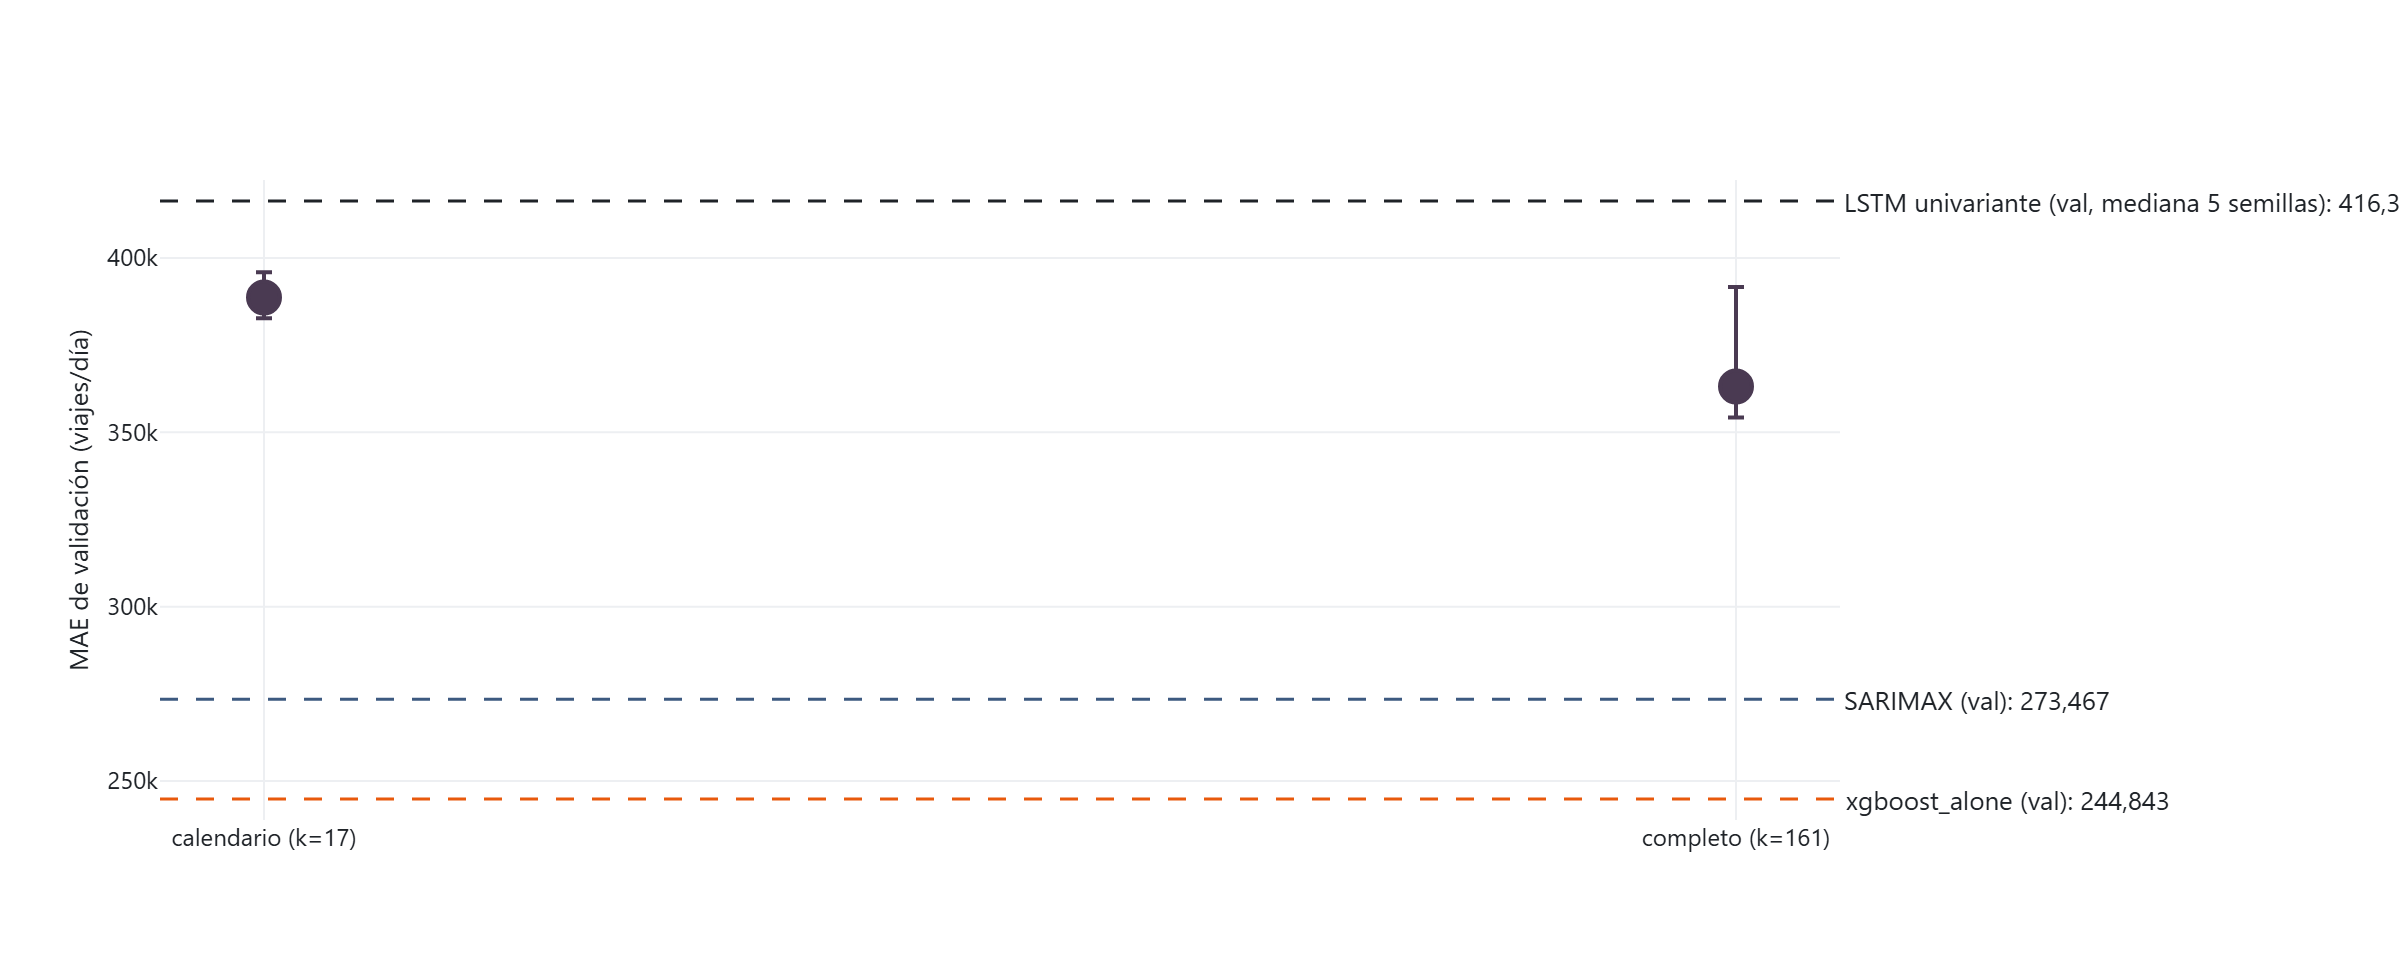
\includegraphics[width=0.78\textwidth]{fig_paridad_lstm.png}
  \caption{\headlinecolor{MAE de validación de la LSTM en paridad informativa por ámbito: mediana y banda mín-máx de 5 semillas, con las líneas de referencia de la LSTM univariante (mediana de 5 semillas), SARIMAX y \texttt{xgboost\_alone} en validación. Ninguno de los dos ámbitos se acerca a la línea de \texttt{xgboost\_alone}.}}
  \label{fig:paridad_lstm}
\end{figure}

\subsection{Lectura conjunta}\label{sec:lectura_conjunta}

Los dos controles apuntan en la misma dirección. La ablación muestra que
\texttt{xgboost\_alone} ya usa de forma medible tanto la información temporal como la
exógena: no hay un componente redundante que la etapa recurrente del híbrido pudiera
aportar por separado. El control de paridad muestra que, aun entregándole a una LSTM
exactamente las variables predictoras que ve XGBoost, e incluso más información en forma de
ventana cruda, la vía recurrente no alcanza a los modelos de una sola etapa. La debilidad
de la etapa 1, por tanto, no parece explicarse en lo esencial por el acceso a la
información: la lectura más plausible es la combinación de una arquitectura recurrente y
unas 860 observaciones diarias, con la salvedad, que el ámbito \texttt{completo} deja
abierta, de que una fracción del hueco pueda deberse también al acceso o a la
representación de la información (sección \ref{sec:limitaciones}).
Esto refuerza, por una vía independiente, la conclusión del contraste central
(\ref{sec:contraste_central}): para la demanda agregada diaria a este tamaño de muestra, un
único modelo de \emph{gradient boosting} sobre una matriz de variables predictoras bien
construida supera a
un híbrido residual secuencial, y el beneficio del híbrido se limita a compensar una etapa
temporal débil en lugar de a batir a modelos de una sola etapa fuertes.

La ablación permite además cerrar una tensión que arrastran las secciones anteriores.
Tres hechos sobre la meteorología retardada parecen
incompatibles: la sección \ref{sec:importancia_variables} reporta que ese bloque concentra
el 51,6\,\% de la ganancia del modelo residual; la sección
\ref{sec:residuo_meteo_anatomia} no encuentra ninguna de sus 105 variables con correlación
parcial significativa con el residuo; y la ablación de la sección
\ref{sec:ablacion_bloques} muestra que retirarlo por completo \emph{mejora} el MAE de
validación en un 3,2\,\% (237.040 frente a 244.843).

La reconciliación está en qué mide
realmente la ganancia por impureza. Esa métrica acumula la reducción de impureza sobre
\emph{cada corte} en que interviene una variable y, por tanto, premia sistemáticamente a
las variables continuas de alta cardinalidad: una columna meteorológica continua ofrece al
algoritmo centenares de puntos de corte candidatos, mientras que una indicadora binaria de
calendario ofrece exactamente uno. Con 105 columnas continuas frente a 17 indicadoras y
solo 552 filas de entrenamiento OOF, el bloque meteorológico dispone de una enorme
superficie de corte sobre la que ajustar ruido, y acumula cuota de ganancia sin aportar
señal explotable. Leídos así, los tres hechos dejan de estar en conflicto y el 51,6\,\% no
es una anomalía, sino \textbf{evidencia adicional a favor de la tesis de este capítulo}: la
etapa 2 dedicó la mayor parte de su capacidad de modelado a un bloque de variables que dos
pruebas independientes (una correlacional, otra de retirada) muestran que no aporta nada.
Es coherente con ello que la variable individual de mayor ganancia del modelo residual siga
siendo \texttt{feat\_day\_type\_festivo} (0,125, sección \ref{sec:importancia_variables}):
el mismo fenómeno visto por el otro lado, con la única variable genuinamente informativa
siendo una indicadora de baja cardinalidad cuya cuota \emph{de grupo} queda diluida. La
conclusión metodológica, aplicable más allá de este TFM, es que una cuota de ganancia por
impureza no es evidencia de utilidad predictiva y no debe leerse como tal sin un
contraste de retirada que la respalde.

\section{Desglose por subgrupos y periodos}\label{sec:desglose_subgrupos}

El contraste central deja abierta una pregunta concreta: aunque el híbrido no gane globalmente, podría
comportarse de forma distinta en festivos, puentes, fines de semana o periodos de demanda
anómala. Esta sección la responde de forma sistemática. Bajo el mismo régimen de
control diagnóstico declarado en la sección \ref{sec:anatomia_residuo_etapa1}, es un
reanálisis puro de \texttt{data/\allowbreak{}processed/\allowbreak{}*\_predictions.parquet}:
no se entrena, reajusta ni vuelve a predecir nada, y todas las cifras proceden de
\texttt{metrics.all\_metrics}, la misma ruta que el resto del capítulo.

El riesgo dominante aquí no es la incompletitud, es la búsqueda selectiva de significación (\emph{p-hacking}): buscar subgrupos
hasta encontrar uno que favorezca al híbrido es \emph{p-hacking} con independencia de por
qué se emprenda la búsqueda. Por eso el diseño se fijó \textbf{antes} de calcular ningún MAE, clasificación
o diferencia —solo se contaron los tamaños muestrales—, de modo que ``el híbrido no gana en
ningún subgrupo'' tenga el mismo estatuto que cualquier hallazgo positivo.

\subsection{Diseño prerregistrado}\label{sec:desglose_diseno}

Se fijaron \textbf{quince subgrupos} como constantes de módulo en
\texttt{src/\allowbreak{}evaluation/\allowbreak{}subgroup\_breakdown.py}, construidos a partir de columnas ya
presentes en \texttt{features\_daily.parquet} (\texttt{day\_type}, \texttt{feat\_is\_bridge\_day},
\texttt{feat\_is\_weekend}, \texttt{holiday\_name}): regímenes de calendario (laborable
ordinario, laborable en puente, sábado, domingo, festivo y sus uniones), estación (julio y
agosto frente al resto del año), dos ventanas ancladas en festivo (22 dic--6 ene; Jueves
Santo $\pm$4 días) y demanda anómala. Un día es \emph{anómalo} si
$\lvert \text{total}_t - \text{total}_{t-7}\rvert$ supera $3{,}0$ desviaciones robustas,
con la escala (MAD) estimada \textbf{solo sobre train} para no ajustar la definición a los
datos de evaluación. La regla alternativa de mediana móvil a 28 días se prototipó sobre
train y se descartó: en ella domina la estacionalidad semanal, con lo que sería un
detector de fines de semana que duplicaría en silencio el subgrupo \texttt{domingo}. Esa
variante no se reporta.

El umbral de inferencia es $n \geq 20$ (\texttt{MIN\_N\_INFERENTIAL}), justificado por el
apalancamiento de un solo día: a $n=20$ un día pesa $\leq$5\,\% de la media del grupo; a
$n=5$, un 20\,\%; a $n=3$, un 33\,\%. Cualquier subgrupo por debajo de 20 se calcula y se
tabula con su $n$, se marca ``no inferencial'' y queda excluido de toda afirmación de
victoria o derrota.

\textbf{Test es la partición de veredicto; validación es el requisito de réplica.} Un
subgrupo cuenta como victoria del híbrido solo si este queda primero en \textbf{ambas}
particiones. Este es el dispositivo anti-\emph{p-hacking} más fuerte del diseño: convierte
una búsqueda de nueve subgrupos en una que exige réplica independiente, y no cuesta nada
porque las dos particiones ya están publicadas. La partición combinada \texttt{val\_test}
(393 días contiguos) es un ámbito \textbf{secundario} prerregistrado, usado solo de forma
descriptiva para los subgrupos que no alcanzan $n=20$ en test; su coste es que el orden
SARIMAX, los hiperparámetros de XGBoost y los pesos del ensamble se eligieron sobre
validación, así que sus resultados se etiquetan como secundarios y nunca encabezan una
conclusión.

\textbf{Resolución del ámbito de veredicto para \texttt{demanda\_anomala}.} Este subgrupo
, el único fijado por nombre en el diseño prerregistrado, tiene $n=16$ en test y $n=34$ en
validación, y su vista combinada \texttt{val\_test} alcanza $n=50$. Recibe el veredicto
\emph{no inferencial} en el ámbito de veredicto (test), exactamente igual que cualquier
otro subgrupo por debajo del umbral, \textbf{sin excepción}. Su resultado combinado se
reporta como ámbito secundario y descriptivo, con la salvedad completa ya indicada, y
nunca porta un veredicto ni un titular. El ámbito combinado estaba disponible y
\textbf{deliberadamente no} se promovió a ámbito de veredicto para este subgrupo: elegir
por subgrupo qué partición decide es un grado de libertad del investigador, y adoptarlo
precisamente para el subgrupo fijado de antemano es donde menos defendible
sería. La función de veredicto lee la constante \texttt{VERDICT\_SCOPE} de forma uniforme
para los quince subgrupos y ningún camino de código asigna un ámbito de veredicto por
subgrupo; una prueba automatizada lo fija.

\textbf{Navidad y Semana Santa no admiten conclusión.} La ventana de evaluación de 393
días contiene exactamente una Navidad (solo en validación, $n=16$; test $n=0$) y una
Semana Santa (solo en test, $n=10$; validación $n=0$). Ninguna definición arregla esto: es
una propiedad de la partición, no del umbral. Ambos periodos se reportan de forma
descriptiva, se marcan \emph{no analizable} y no se emite ninguna afirmación de victoria o
derrota sobre Navidad o Semana Santa en este TFM. La lista de subgrupos se fijó por
adelantado y añadir uno tras ver los resultados invalidaría la corrección por comparaciones
múltiples: es la restricción que prevalece sobre la exhaustividad.

\subsection{Resultados por subgrupo}\label{sec:desglose_resultados}

Las tablas \ref{tab:subgrupos_test} y \ref{tab:subgrupos_val} recogen, por subgrupo y para
un conjunto reducido de modelos, el mejor competidor y su MAE, el mejor híbrido y su MAE,
la diferencia entre ambos y el veredicto prerregistrado. La figura
\ref{fig:subgrupos_mae} lo representa con barras huecas para los subgrupos no
inferenciales.

\begin{figure}[htbp]
  \centering
  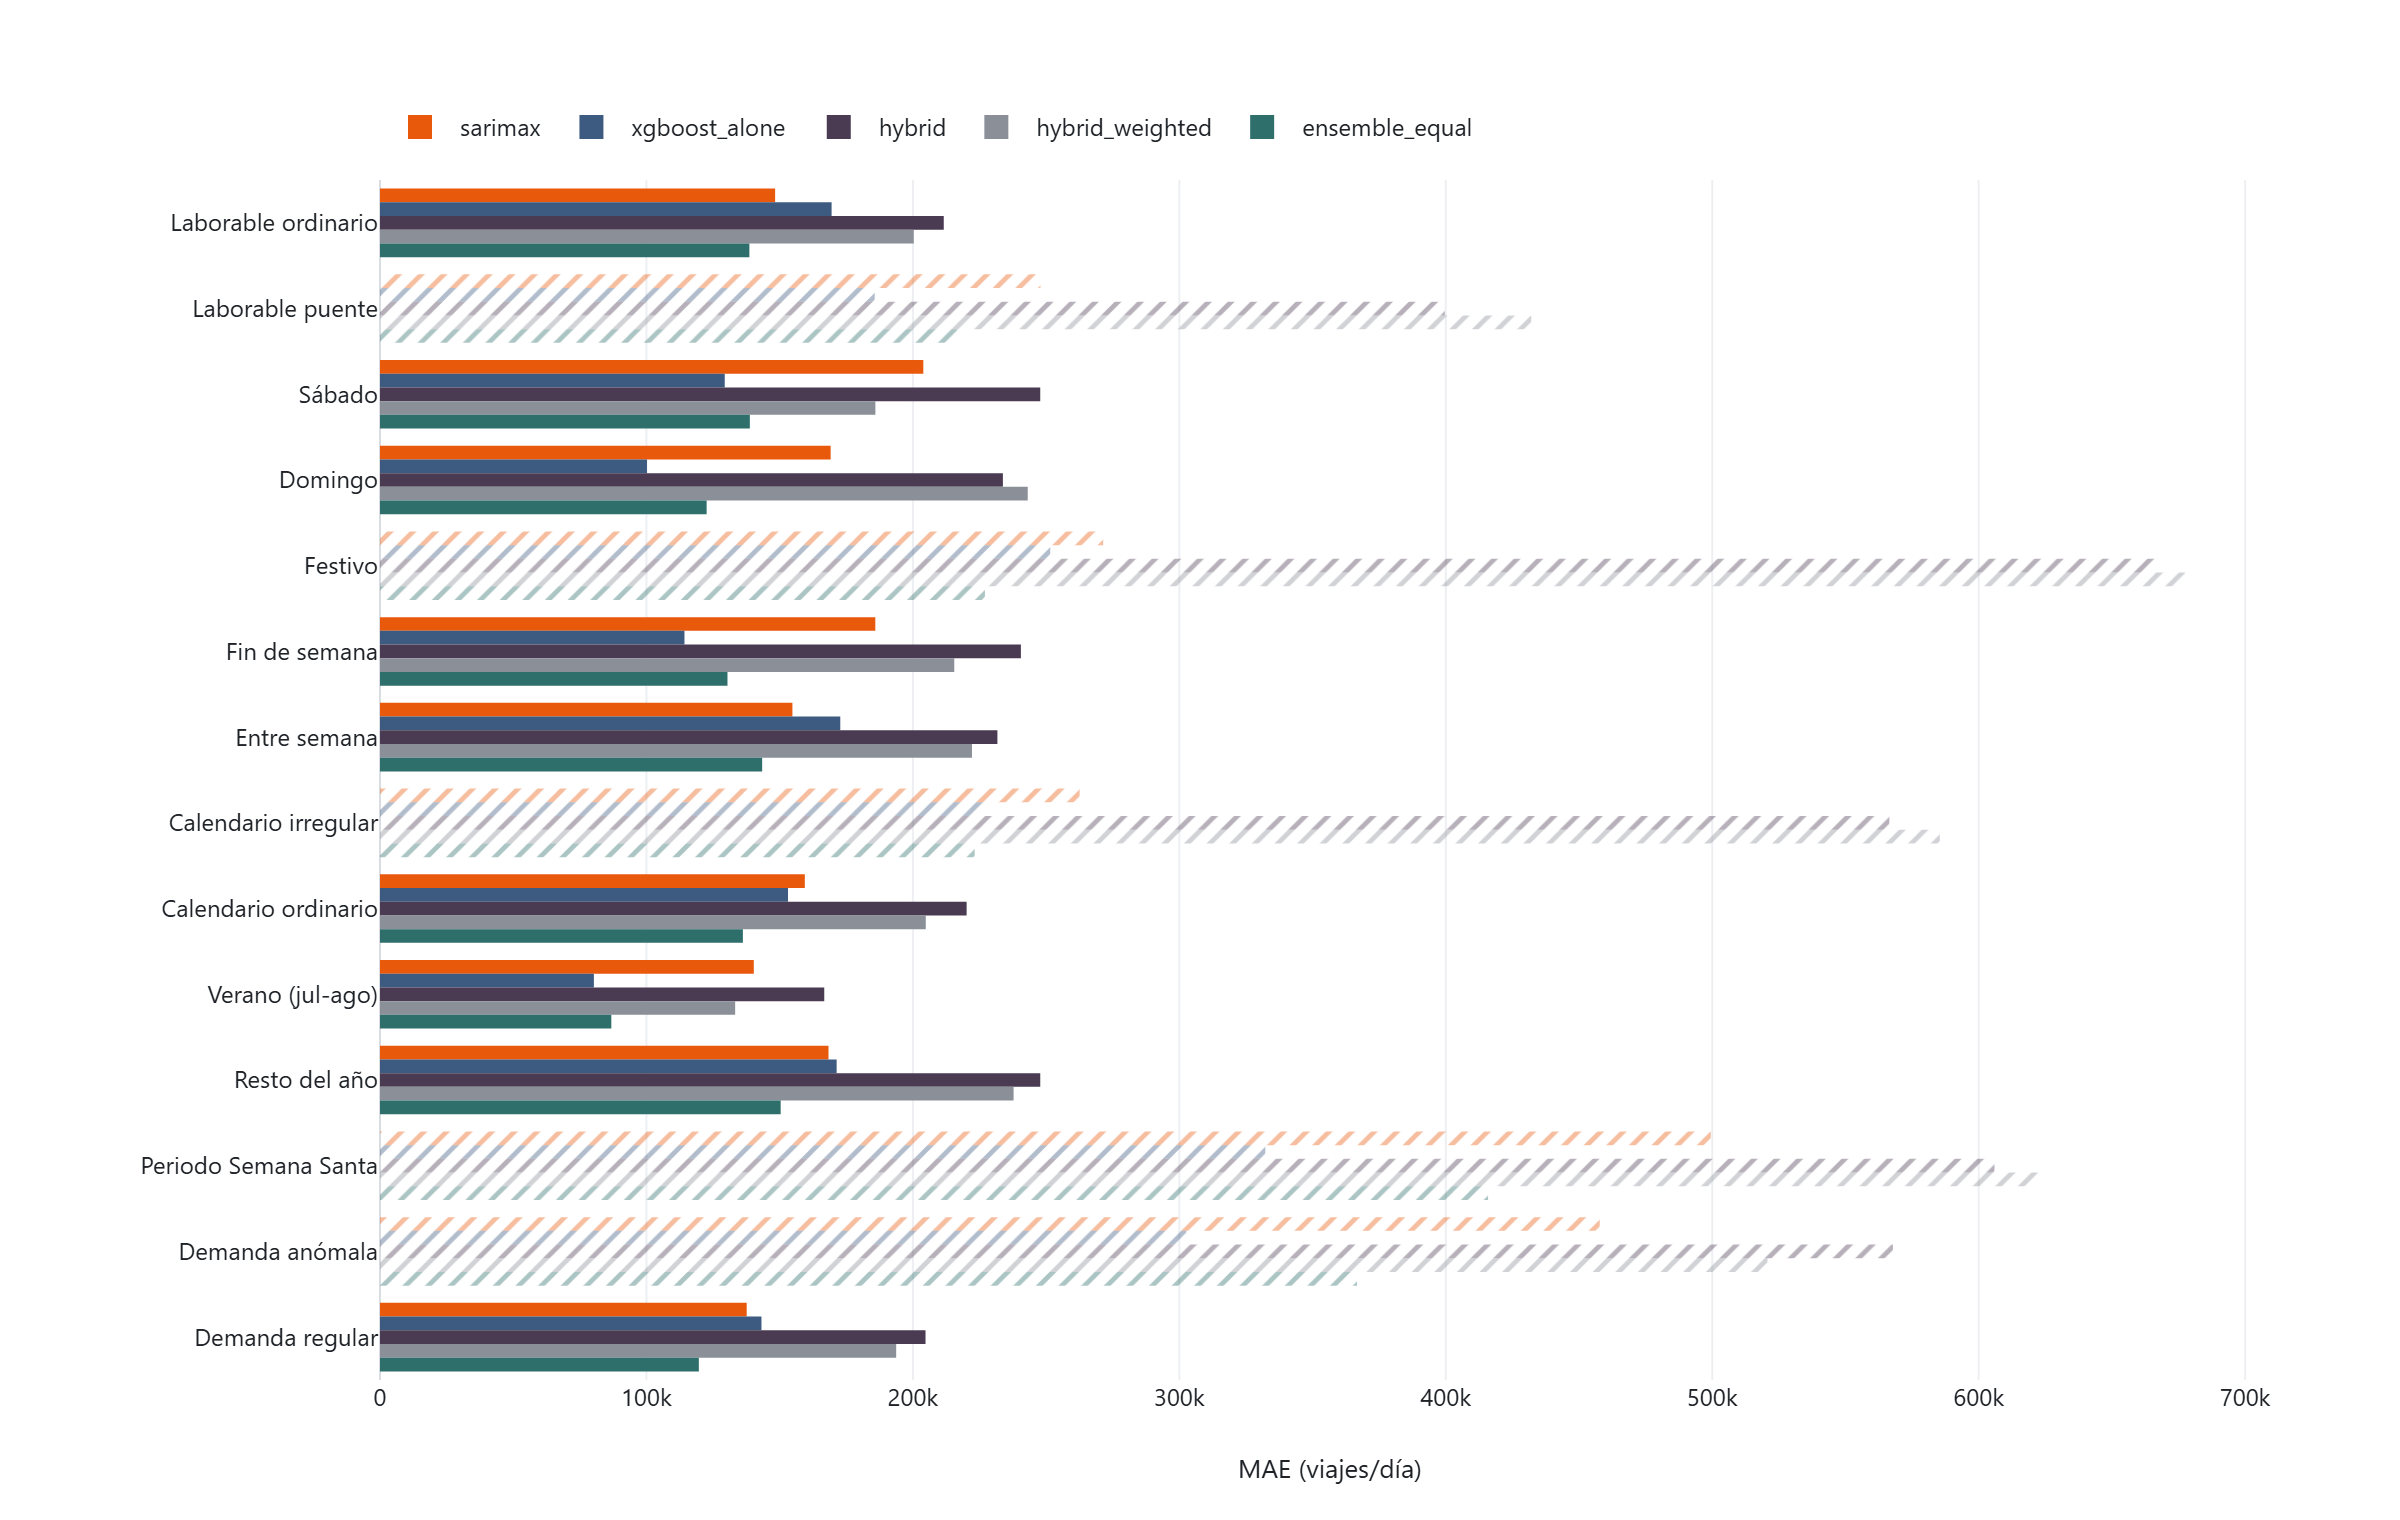
\includegraphics[width=0.78\textwidth]{fig_subgrupos_mae.png}
  \caption{\headlinecolor{MAE por subgrupo en la partición test para el conjunto reducido de modelos. Las barras huecas y traslúcidas corresponden a subgrupos no inferenciales ($n < 20$).}}
  \label{fig:subgrupos_mae}
\end{figure}

El resultado es negativo en todos los subgrupos inferenciales. De los quince subgrupos prerregistrados, nueve alcanzan $n \geq
20$ en test; cuatro quedan por debajo (laborable en puente $n=3$, festivo $n=5$, calendario
irregular $n=8$, demanda anómala $n=16$) y dos están excluidos por falta de solape
val/test. \textbf{En 0 de los 9 subgrupos con $n$ suficiente gana el híbrido con
evidencia}, y en 0 queda siquiera primero sin evidencia: en los nueve, el mejor híbrido es
peor que el mejor competidor por entre 53.019 (verano) y 133.578 (domingo) viajes diarios
de MAE. En validación el único subgrupo donde un híbrido queda primero es festivo ($n=9$),
que es no inferencial y además no replica el hecho en test. La búsqueda se ha completado con
resultado negativo.

El único hallazgo positivo ya conocido se mantiene y se reitera: en festivos, la etapa 2
recorta el error de la etapa 1 de 1.585.388 a 666.572 (un $-58$\,\%). El mecanismo de
corrección residual es real; lo que es insuficiente es la etapa 1 de la que parte, y ese
recorte no convierte a festivo en una victoria de subgrupo —sigue siendo peor que
\texttt{xgboost\_alone} y que el ensamble, y su $n=5$ lo hace indicativo, no concluyente—.

La etiqueta \texttt{demanda\_anomala} usa el $\text{total}_t$ observado: es legítima para un
reporte a posteriori, pero \textbf{ilegítima como regla de enrutamiento}. No cabe concluir
de ello que el híbrido deba desplegarse en los días anómalos: la anomalía no se conoce
antes de observar la demanda del propio día. Su vista combinada \texttt{val\_test}
($n=50$, secundaria y descriptiva) tampoco cambia el signo: el mejor híbrido es peor que
\texttt{xgboost\_alone} por unos 123.000 de MAE.

\subsection{Incertidumbre y comparaciones múltiples}\label{sec:desglose_incertidumbre}

La incertidumbre de cada diferencia se obtiene con un remuestreo \emph{bootstrap} pareado de bloques
móviles. Como un subgrupo categórico está disperso por la partición, el remuestreo se hace
sobre la serie de evaluación completa y contigua, en bloques de 7 días (preservan la
dependencia semanal, que es la autocorrelación dominante y la razón por la que un contraste
pareado ingenuo sobreestima la significación), con 2000 réplicas y semilla global. La
pertenencia al subgrupo viaja con el día, y \texttt{best\_model} y \texttt{best\_hybrid} se
\textbf{vuelven a seleccionar dentro de cada réplica} (\emph{argmin} sobre competidores y
sobre \{\texttt{hybrid}, \texttt{hybrid\_weighted}\}), de modo que la doble selección se
paga en lugar de ignorarse. Una réplica que aporta menos de 20 días del subgrupo se
descarta; si la fracción de réplicas utilizables baja de $0{,}90$, el intervalo de
confianza se suprime. El cuadro \ref{tab:subgrupos_inferencia} recoge la diferencia, su
intervalo y las dos p, bruta y ajustada, para cada subgrupo de la familia inferencial, y
la figura \ref{fig:subgrupos_delta_ic} representa esas mismas diferencias como gráfico de
bosque frente a la línea del cero.

\begin{figure}[htbp]
  \centering
  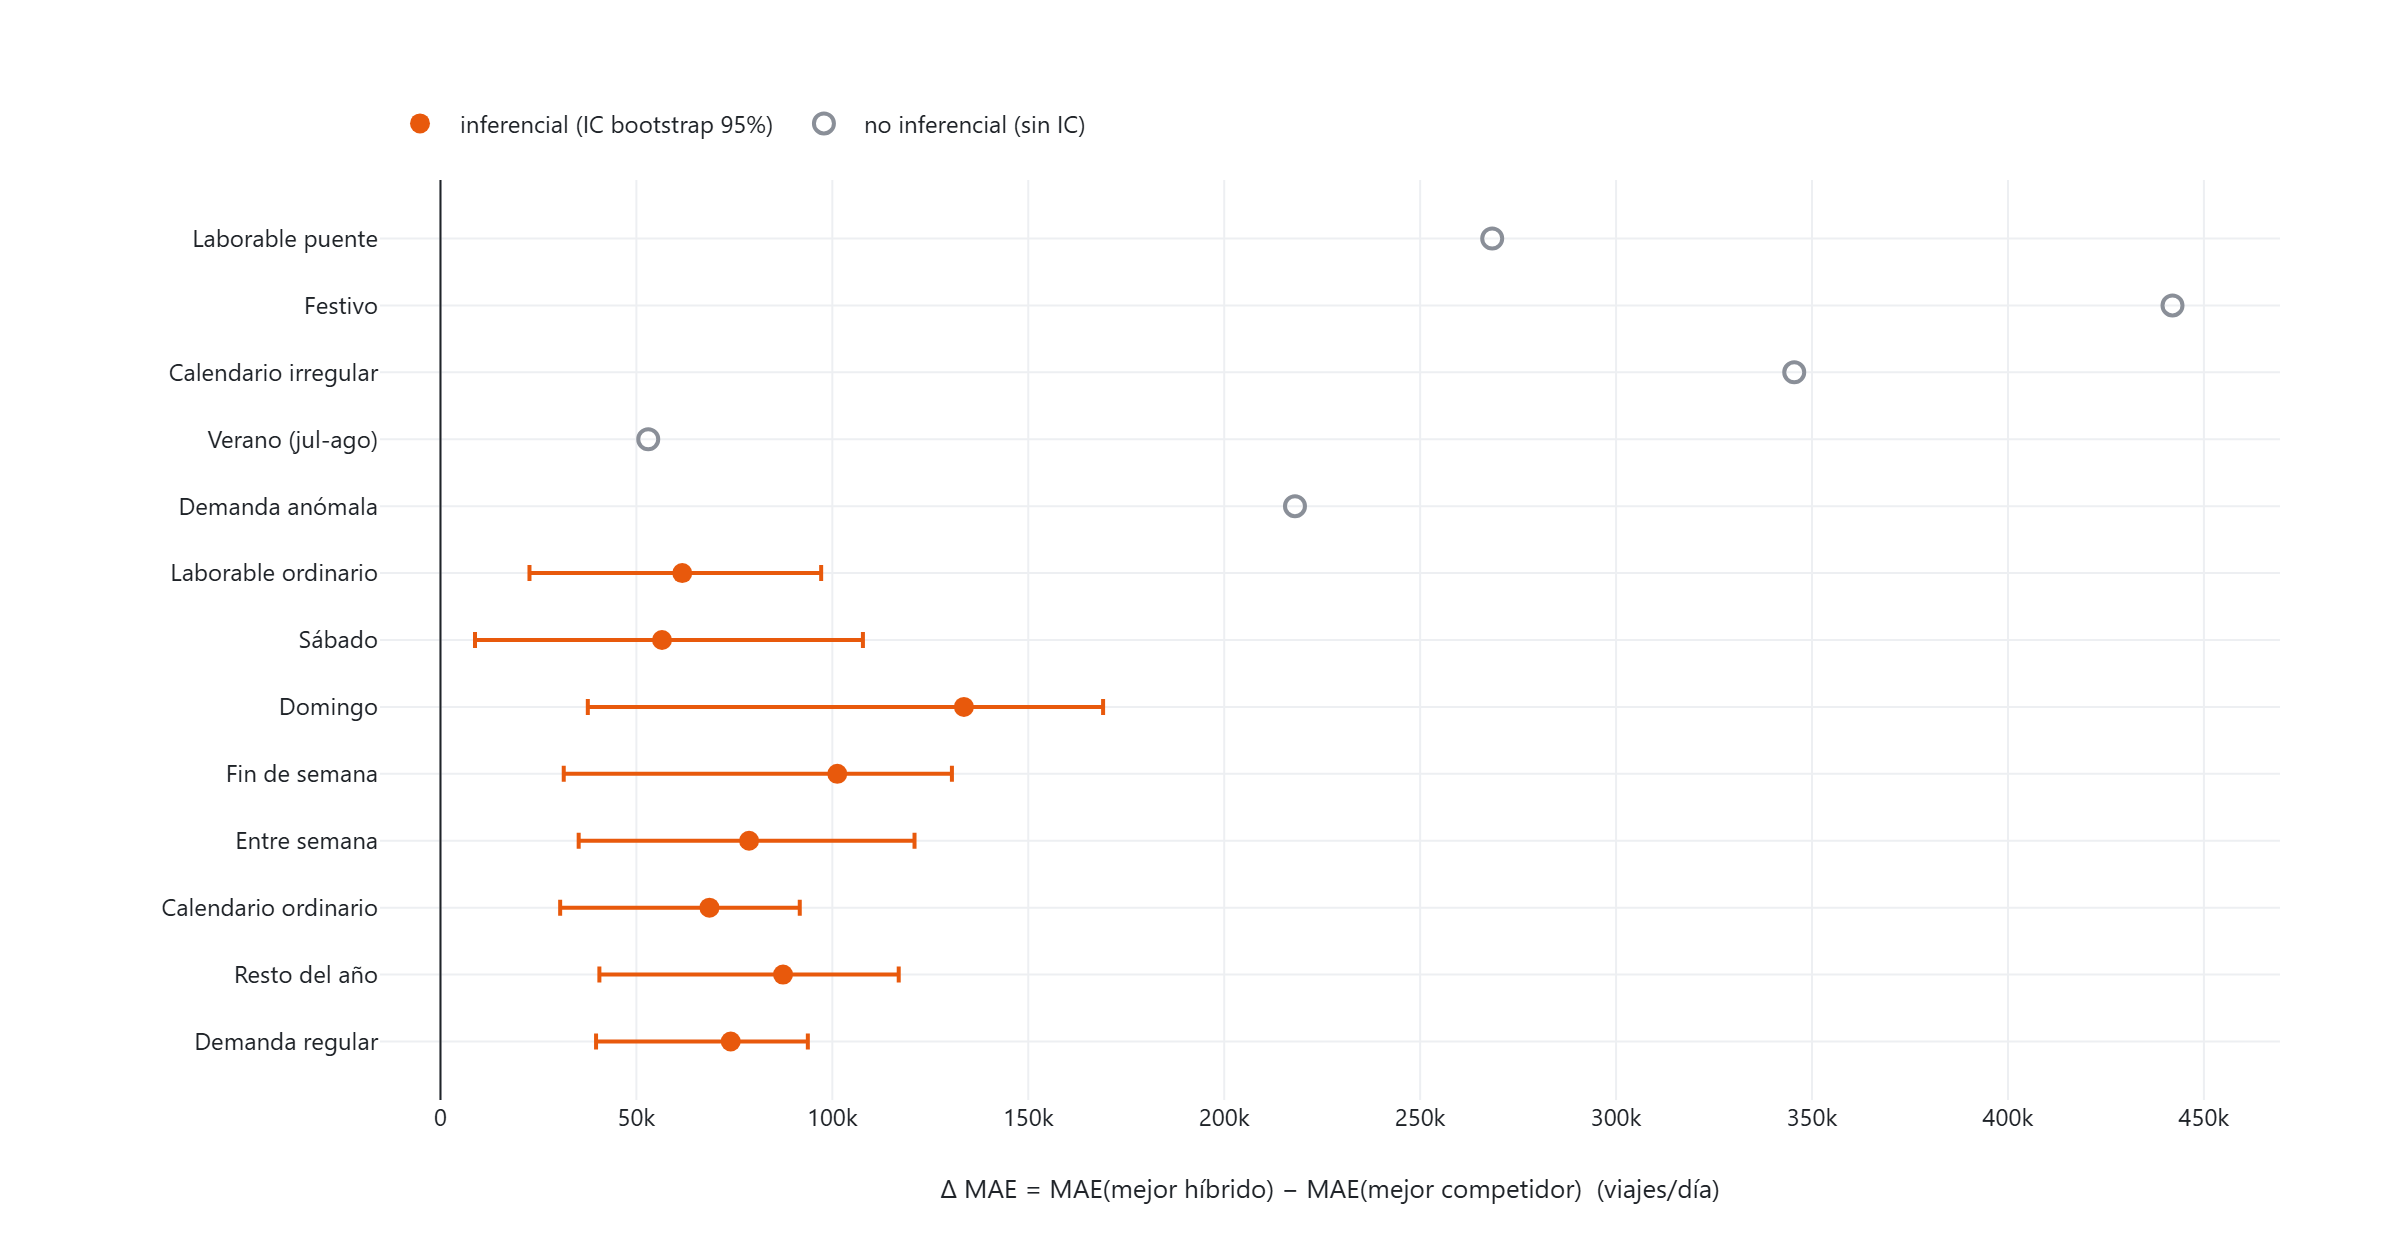
\includegraphics[width=0.78\textwidth]{fig_subgrupos_delta_ic.png}
  \caption{\headlinecolor{Gráfico de bosque de la diferencia de MAE por subgrupo con su IC \emph{bootstrap} del 95\,\%. La línea del cero es la referencia: un IC íntegramente a su derecha es evidencia de que el híbrido pierde en ese subgrupo. Marcadores huecos y sin IC para los subgrupos no inferenciales.}}
  \label{fig:subgrupos_delta_ic}
\end{figure}

La corrección de Benjamini-Hochberg se aplica con la misma llamada y el mismo $q=0{,}10$
que el análisis meteorológico de la sección \ref{sec:anatomia_residuo_etapa1}, sobre la
familia de los nueve subgrupos inferenciales (una hipótesis por subgrupo, no una por
subgrupo$\times$modelo, porque el estadístico focal es una única diferencia). Los subgrupos
se solapan fuertemente (\texttt{entre\_semana} contiene a \texttt{laborable\_ordinario}),
así que los contrastes son positivamente dependientes —el régimen (PRDS) bajo el que
\texttt{fdr\_bh} sigue siendo válido—; las diferencias entre subgrupos \textbf{no
descomponen}: es una familia de vistas solapadas, no una partición.

En los nueve subgrupos inferenciales la diferencia es positiva y significativa tras
Benjamini-Hochberg: la evidencia es que el híbrido es significativamente \textbf{peor}, no
que empate. Este es el desenlace más expuesto a sobrelectura, así que su tratamiento —la
corrección sobre la familia inferencial y el requisito de réplica en validación— está
prerregistrado. Donde la inferencia es
imposible —festivo ($n=5$), laborable en puente ($n=3$)— no se realiza inferencia
estadística debido al reducido tamaño muestral: se reporta únicamente el MAE puntual con
su $n$.

\subsection{Vista temporal}\label{sec:desglose_temporal}

La figura \ref{fig:mae_movil_periodo} traza, sobre los 393 días contiguos de validación y
test, el MAE móvil a 28 días de cada modelo (panel superior) y la diferencia móvil entre el
mejor híbrido y el mejor competidor (panel inferior), con la frontera val/test marcada. La
ventana de 28 días se hereda de $W=28$ de la LSTM y de la ventana de las variables móviles;
no se ha ajustado. La diferencia móvil se mantiene por encima de cero en toda la serie: la
posición relativa del híbrido no se invierte en ningún tramo. Es una figura descriptiva:
ventanas consecutivas se solapan en 27 días, así que no se le aplica ningún contraste y las
ventanas que cruzan la frontera mezclan las dos particiones.

\begin{figure}[htbp]
  \centering
  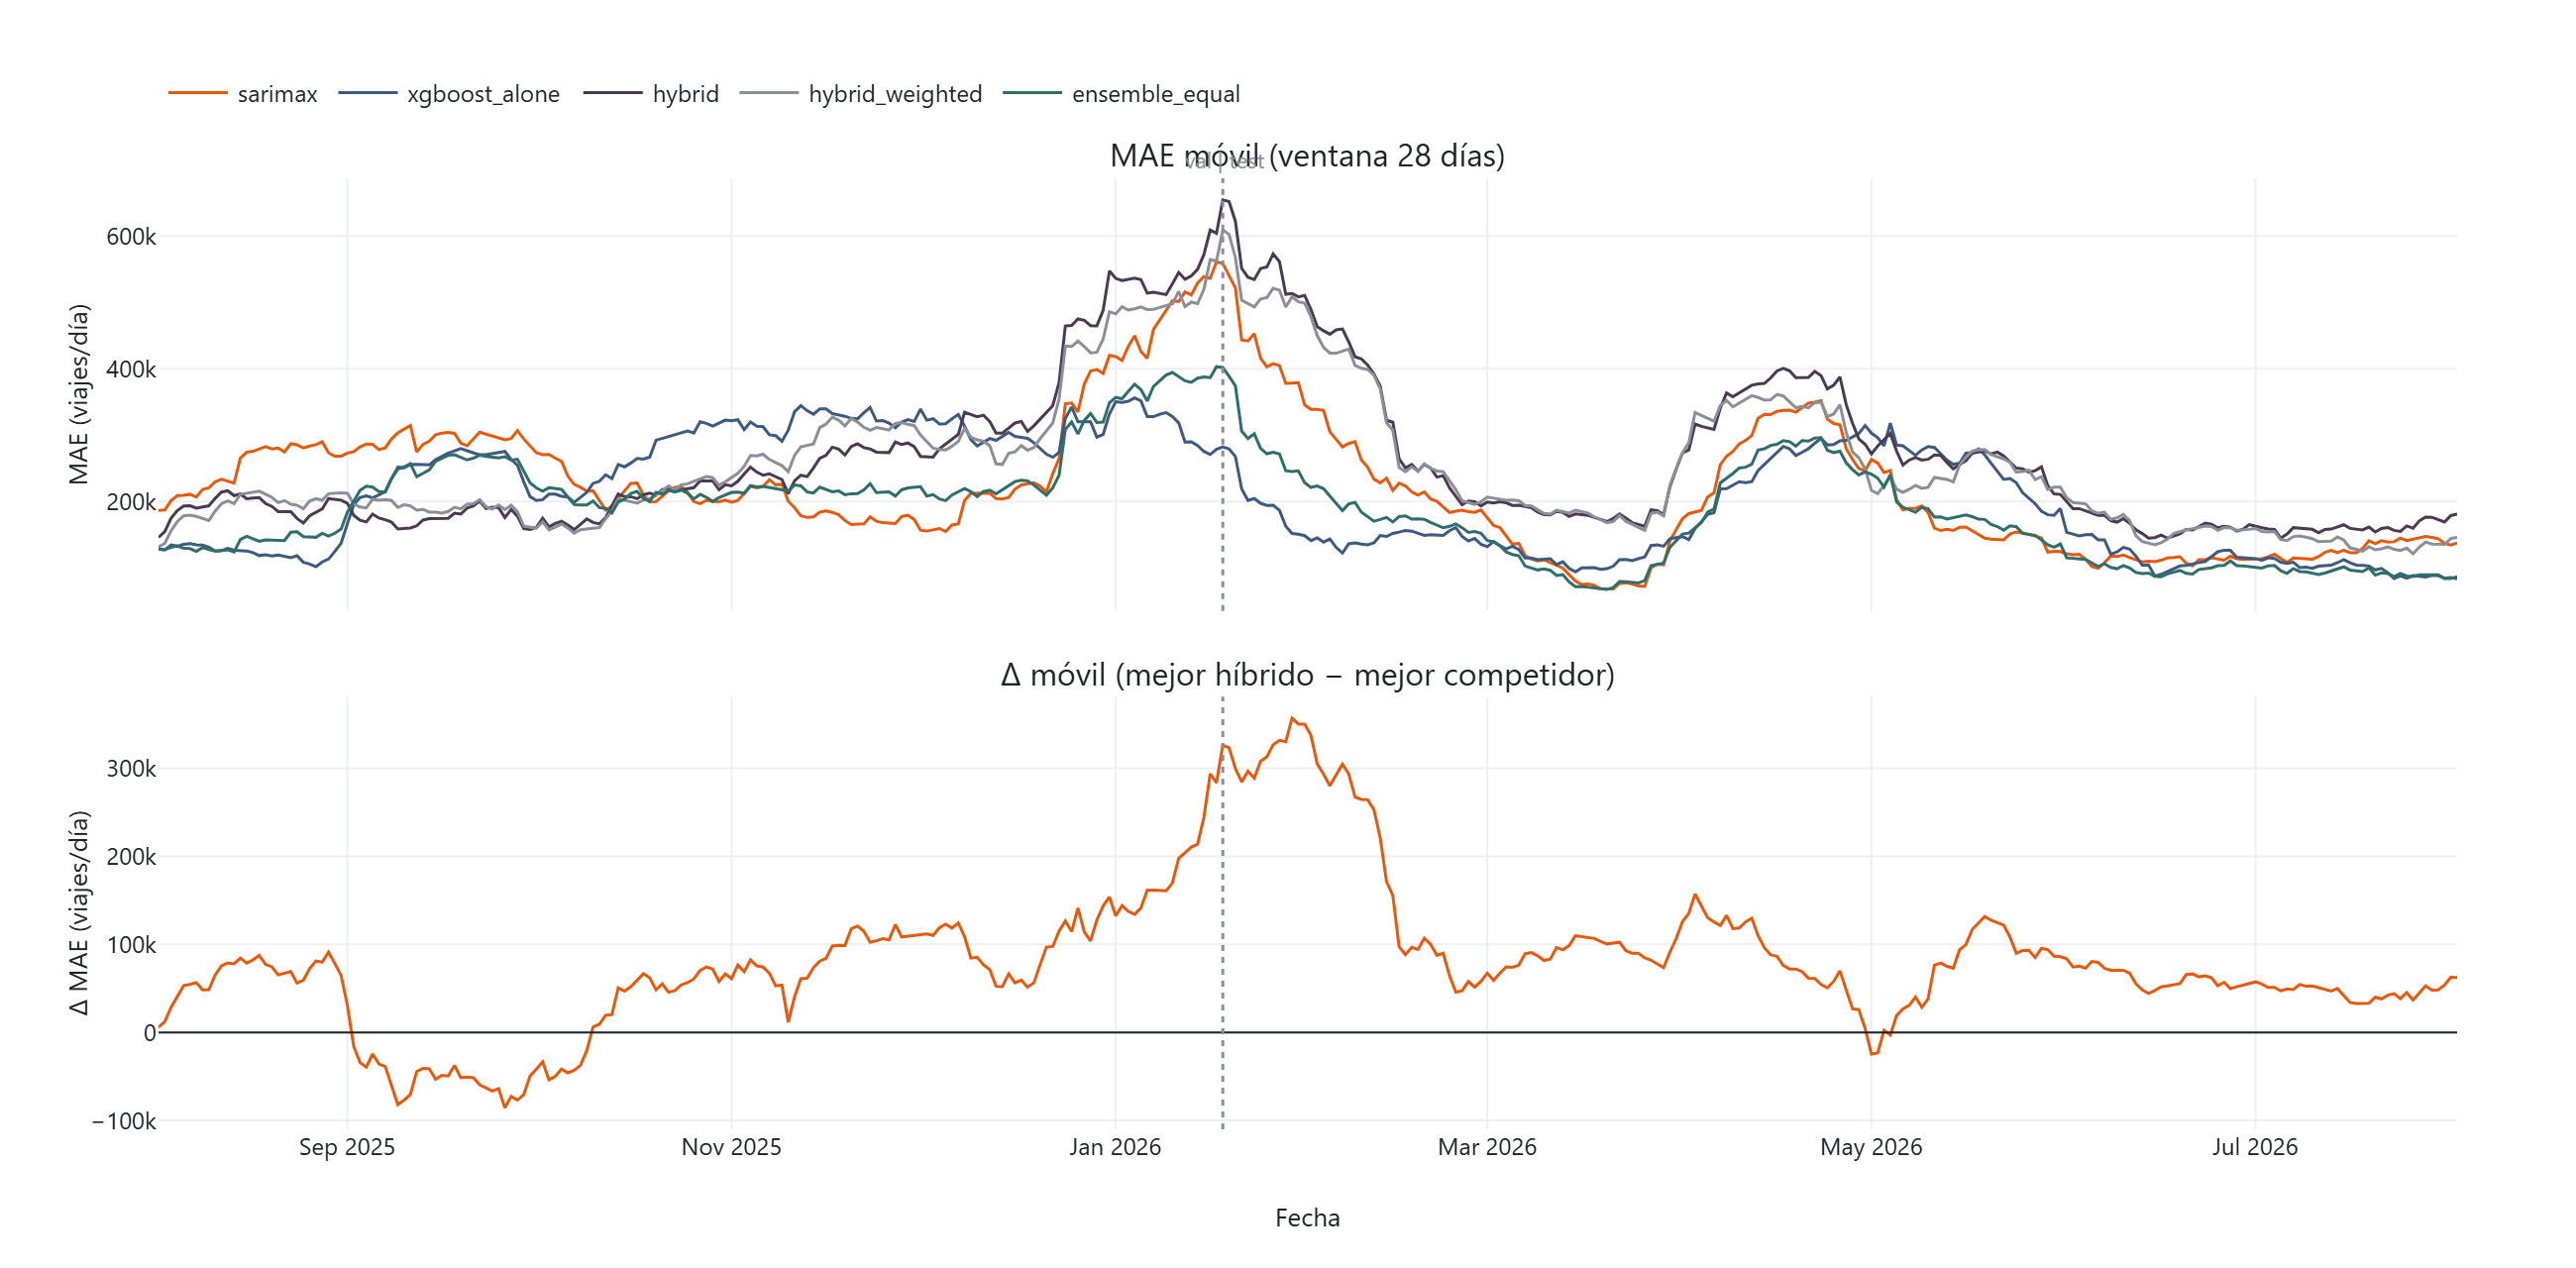
\includegraphics[width=0.78\textwidth]{fig_mae_movil_periodo.png}
  \caption{\headlinecolor{MAE móvil a 28 días por modelo (panel superior) y diferencia móvil mejor híbrido $-$ mejor competidor (panel inferior) sobre la ventana contigua de validación y test. Regla vertical en la frontera val/test. Figura descriptiva: sin contraste, por el fuerte solapamiento de ventanas consecutivas.}}
  \label{fig:mae_movil_periodo}
\end{figure}

\subsection{Lectura}\label{sec:desglose_lectura}

La búsqueda por subgrupos y periodos se ha completado con un
resultado negativo bien instrumentado. En los nueve subgrupos con tamaño muestral
suficiente el híbrido \textbf{no queda primero en ninguno}, ni con evidencia ni sin ella, y en los
nueve la evidencia \emph{bootstrap}, corregida por comparaciones múltiples, es que es
significativamente peor que el mejor modelo de una sola etapa o el ensamble. En los cuatro
subgrupos no inferenciales, incluido el de demanda anómala, no se emite veredicto. El único comportamiento diferencial real del híbrido, el recorte del
$58$\,\% del error de la etapa 1 en festivos, es un mecanismo de corrección, no una
victoria, y ya estaba documentado. Esta sección no abre preguntas de investigación nuevas:
cierra la que quedaba, confirmando por una vía sistemática la respuesta del contraste
central (\ref{sec:contraste_central}).

\section{Respuesta a las preguntas de investigación}\label{sec:respuesta_preguntas}

Se retoman aquí, en el mismo orden en que se plantearon en la sección
\ref{sec:preguntas_investigacion}, las cinco preguntas de investigación que estructuran
este TFM, respondidas de forma explícita y remitiendo a la evidencia ya presentada en
este capítulo.

\begin{description}[nosep,leftmargin=0pt,labelindent=0pt,style=nextline,font=\bfseries]
  \item[PI1. ¿Bate el híbrido a SARIMAX en validación y en test simultáneamente?]
    No, en ninguna de las dos particiones: el MAE del híbrido es 7.270 viajes diarios peor
    en validación y 70.597 peor en test (tabla \ref{tab:delta_hibrido}, sección
    \ref{sec:contraste_central}).

  \item[PI2. ¿Bate el híbrido a \texttt{xgboost\_alone}, entrenado sobre las mismas
    variables predictoras?]
    No, y por un margen todavía mayor que frente a SARIMAX: 35.895 en validación y 78.103
    en test (tabla \ref{tab:delta_hibrido}).

  \item[PI3. ¿Reduce el híbrido específicamente el error en festivos y puentes frente a
    SARIMAX y \texttt{xgboost\_alone}?]
    No: es peor que ambos en prácticamente todos los grupos de calendario de la tabla
    \ref{tab:desglose_dia_test}, con la salvedad de que la comparación en festivos (n=5) y
    puentes (n=3) en la partición test debe leerse como indicativa, no concluyente, dado su
    reducido tamaño muestral (sección \ref{sec:error_dia}).

  \item[PI4. ¿Funciona la etapa 2 como mecanismo de corrección residual, aunque el
    híbrido completo no supere a los modelos de una sola etapa?]
    Sí: reduce el MAE de la etapa 1 en un 16,6\,\% en test y, de forma más marcada todavía,
    en un 58\,\% en festivos, de 1.585.388 a 666.572 (sección \ref{sec:error_dia}), y la
    variable de mayor ganancia del modelo residual, \texttt{feat\_day\_type\_festivo}
    (0,125), apunta, a nivel de variable individual, a que esa corrección procede
    de la señal de calendario que la etapa 1 no puede ver (sección
    \ref{sec:importancia_variables}). El mecanismo de la arquitectura híbrida es real; lo
    que resulta insuficiente es la etapa 1 de la que parte.

  \item[PI5. ¿Existe una combinación más simple que supere a ambos componentes de una
    sola etapa?]
    Sí: el ensamble equiponderado 50/50 de SARIMAX y \texttt{xgboost\_alone}
    (\texttt{ensemble\_equal}), sin ninguna red LSTM ni reentrenamiento adicional, alcanza
    un MAE de test de 139.725; su variante ponderada por el inverso del MAE de validación
    (\texttt{ensemble\_inverse\_mae}, pesos 0,4724/0,5276) lo reduce ligeramente a 139.681,
    un 10,5\,\% por debajo del mejor de sus dos componentes, en consonancia con la
    descorrelación de errores entre ambos (sección \ref{sec:mecanismo_ensemble}).
\end{description}

Los dos controles diagnósticos de la sección \ref{sec:paridad_informativa} no abren
preguntas de investigación nuevas, pero refuerzan las respuestas a PI1, PI2 y PI4 por una
vía independiente: la ablación de bloques (\ref{sec:ablacion_bloques}) confirma
mecánicamente que \texttt{xgboost\_alone} ya integra la información temporal y la exógena
—lo que explica por qué separar el problema en dos etapas no añade poder predictivo—, y el
control de paridad informativa (\ref{sec:paridad_lstm}) reduce la plausibilidad de que la
desventaja de la etapa 1 se explique únicamente por su carácter univariante: sigue por
detrás de los modelos de una sola etapa incluso viendo las mismas variables predictoras que
XGBoost (veredicto \emph{limitación arquitectónica} en \texttt{calendario}). No obstante,
el ámbito \texttt{completo} presenta un resultado \emph{mixto/ambiguo}, por lo que no puede
descartarse que parte de la diferencia esté relacionada también con el acceso o la
representación de la información (sección \ref{sec:limitaciones}).

\chapter{Conclusiones y trabajos futuros}\label{cap:conclusiones}

Este capítulo de cierre no introduce ninguna cifra nueva: toda afirmación que sigue
remite a una tabla o figura ya presentada y discutida en el capítulo
\ref{cap:resultados}, del que este capítulo es una síntesis argumental y no una nueva
fuente de evidencia.

\section{Conclusiones}\label{sec:conclusiones}

El objetivo general —evaluar si una arquitectura híbrida residual LSTM-XGBoost mejora la
predicción de la demanda diaria agregada de transporte público en Madrid frente a
baselines estadísticos y a modelos de una sola etapa— se ha cumplido: la evaluación se
realizó y su respuesta es negativa para la arquitectura. El cumplimiento de cada objetivo
específico de la sección \ref{sec:objetivos} se acredita por separado:

\begin{itemize}
  \item \textbf{OE1, ingesta y matriz anti-fuga.} \emph{Qué se hizo:} tres fuentes crudas
    unificadas en 1.310 días continuos y una matriz de 161 variables predictoras con
    guardias que fallan de forma explícita (capítulo \ref{cap:datos_features}).
    \emph{Resultado:} ninguna guardia ha detectado una fuga en la matriz publicada; las
    dos que durante varias fases eran inalcanzables se corrigieron y disparan hoy bajo
    prueba (Anexo \ref{cap:anexo2}). \emph{Cumplido.} \emph{Limitación:} la ausencia
    total de fuga no puede afirmarse sin una auditoría exhaustiva externa (sección
    \ref{sec:limitaciones}).
  \item \textbf{OE2, baselines y SARIMAX.} \emph{Qué se hizo:} cuatro baselines ingenuos y
    un SARIMAX(2,1,2)$\times$(0,1,2,7) seleccionado por AIC de entrenamiento, todos a un
    día vista (sección \ref{sec:baselines}). \emph{Resultado:} SARIMAX alcanza un MAE de
    test de 163.627 y es uno de los dos modelos de una sola etapa más precisos: se
    incorpora como un modelo de referencia competitivo y metodológicamente relevante
    (PI1, PI2). \emph{Cumplido.} \emph{Limitación:}
    el orden elegido no está fuertemente identificado (cinco órdenes en 0,8 unidades de
    AIC).
  \item \textbf{OE3, etapa 1 con predicciones OOF.} \emph{Qué se hizo:} LSTM univariante
    con esquema \emph{walk-forward} expansivo de cinco folds y escalador reajustado por fold
    (sección \ref{sec:esquema_oof}). \emph{Resultado:} 689 predicciones OOF sobre 889 filas;
    el fold 1 resultó degenerado y se excluyó tras comprobar su cobertura.
    \emph{Cumplido.} \emph{Limitación:} el residuo de entrenamiento procede de modelos con
    337-748 filas mientras que el de inferencia procede del modelo con 889, un
    desplazamiento inherente al \emph{stacking} OOF.
  \item \textbf{OE4, etapa 2 y controles.} \emph{Qué se hizo:} XGBoost sobre 552 residuos
    OOF con las 161 variables, comparado con la etapa 1 sola y con un XGBoost directo sobre
    la misma matriz (secciones \ref{sec:etapa2_xgboost} y \ref{sec:modelos_control}).
    \emph{Resultado:} la etapa 2 reduce el MAE de su etapa 1 en un 16,6\,\% en test, pero
    el híbrido queda por detrás de SARIMAX y de XGBoost independiente en ambas
    particiones (PI3, PI4). \emph{Cumplido en su formulación} —el contraste se realizó y
    los controles aislaron la causa—, \emph{con resultado negativo}. \emph{Limitación:}
    5 festivos y 3 puentes en test impiden concluir sobre los días irregulares.
  \item \textbf{OE5, ensamble, sensibilidad e interpretación.} \emph{Qué se hizo:} dos
    experimentos acotados y una lectura a la luz de \textcite{granger1989combining}
    (sección \ref{sec:analisis_sensibilidad}). \emph{Resultado:} el repesado no mejora los
    días que perseguía; el ensamble aritmético de SARIMAX y XGBoost independiente es el
    modelo más preciso del estudio (PI5). \emph{Cumplido.} \emph{Limitación:} la
    preferencia entre las dos variantes del ensamble se formuló tras conocer sus cifras de
    test (sección \ref{sec:limitaciones}).
\end{itemize}

El hallazgo empírico central aparece en la evaluación de la corrección residual:
\textbf{el híbrido, tal como queda diseñado, no supera a SARIMAX ni a
XGBoost independiente en ninguna de las dos particiones} (PI1 y PI2, tabla
\ref{tab:delta_hibrido}), y tampoco reduce de forma diferencial el error en los días de
calendario irregular que motivaron su diseño (PI3, tabla \ref{tab:desglose_dia_test}).
No es un fallo de ejecución sino un resultado consistente con la teoría de combinación de
pronósticos: \textcite{granger1989combining} exige que los componentes sean
individualmente subóptimos \emph{y} se apoyen en conjuntos de información distintos, y
esta arquitectura no satisface plenamente la segunda condición —los conjuntos de información de sus dos
etapas están anidados, no son complementarios: la etapa 2 añade calendario y meteorología,
pero el pasado reciente que ve la etapa 1 ya está representado en su matriz— como se
argumenta en la sección
\ref{sec:resultado_negativo_teoria}. Las competiciones M4 y M5
\parencite{makridakis2018m4,makridakis2022m5} documentan que el patrón —métodos simples y
combinaciones bien fundamentadas superando a arquitecturas más sofisticadas, sobre todo en
muestras moderadas como las 1.310 observaciones de este proyecto— es esperable y no una
anomalía de esta implementación.

Tampoco debe leerse como una arquitectura sin mérito: PI4 muestra que la etapa 2 cumple
su función, reduciendo el MAE de su propia etapa 1 en un 16,6\,\% en test y un 58\,\% en
festivos; su variable de mayor ganancia, \texttt{feat\_day\_type\_festivo}, es coherente
con que esa corrección proceda de la señal de calendario que una LSTM univariante no puede
ver por construcción (sección \ref{sec:importancia_variables}). El mecanismo que justifica
la hibridación se observa de forma medible; lo insuficiente es la etapa 1 de la que parte.

El modelo que mejor resuelve el problema no requiere ninguna red neuronal: PI5 muestra
que un ensamble aritmético de SARIMAX y XGBoost independiente —sin reentrenamiento, sin
etapa LSTM y sin ningún paso de ajuste— alcanza un MAE de test de 139.725 en su variante
equiponderada (el ensamble 50/50) y de 139.681 en la ponderada por el inverso del MAE
(el ensamble inverso al MAE), en torno a un 10,5\,\% por debajo del mejor de sus
componentes. Es coherente con la identidad de
\textcite{bates1969combination} aplicada a la correlación de 0,576 entre los residuos de ambos
sobre test (sección \ref{sec:mecanismo_ensemble}): inferior a la unidad porque fallan en
subconjuntos de días sistemáticamente distintos —el primero en laborables ordinarios, el
segundo en fin de semana y festivos—, que es lo que hace ventajoso promediarlos.

La lectura conjunta de ambos resultados —el híbrido secuencial que no mejora porque sus
etapas observan conjuntos de información anidados, y el ensamble paralelo que sí mejora, en
consonancia con la combinación de información parcialmente descorrelacionada— es la
aportación empírica central de este TFM:
una auditoría con protocolo \emph{out-of-fold} estricto en toda su cadena de las
condiciones exactas bajo las cuales cada estrategia de combinación funciona y bajo cuáles
no, sobre una serie real de demanda de transporte público agregada y multimodal.

\section{Limitaciones}\label{sec:limitaciones}

\textbf{Agregación a nivel de red, sin corte espacial.} Este proyecto modela la demanda
\texttt{total} del sistema CRTM como una única serie diaria, con el desglose por operador
solo como variable de apoyo (rezagos, EDA) y no como dimensión espacial del modelo. A
diferencia de \textcite{cardozo2012spatial}, que modelan las entradas estación
por estación, esta memoria no ofrece resolución espacial alguna: de sus resultados no cabe
concluir nada sobre una línea, una estación o un corredor concreto. La elección fue
deliberada (sección \ref{sec:movilidad_urbana}), pero es una limitación de alcance.

\textbf{Tamaño muestral reducido en los días de calendario más interesantes.} Con 1.310
observaciones diarias en total, la muestra es modesta para un modelo LSTM, y se vuelve
particularmente escasa precisamente en los subgrupos de calendario cuyo comportamiento
resulta más interesante para este estudio: la partición de test contiene solo 5 días
festivos y 3 días de laborable con puente (tabla \ref{tab:desglose_dia_test}). Todas
las afirmaciones de esta memoria sobre el comportamiento de los modelos en esos dos
grupos, incluida la mejora del 58\,\% de la etapa 2 sobre su etapa 1 en festivos, se han
etiquetado consistentemente como indicativas y no concluyentes; la base más sólida para
generalizar sobre el comportamiento estructural frente al calendario sigue siendo el
diagnóstico exploratorio de la fase 4 sobre el periodo completo (48 festivos y 54
puentes; la detección de calendario identifica 55 días puente sobre los 1.310 días
totales, de los que 54 caen fuera de los 28 días de calentamiento excluidos del
entrenamiento), no las particiones reducidas de evaluación final.

\textbf{Recorte de 28 días por calentamiento de las variables de retardo.} El retardo y la
media móvil de mayor ventana (28 días) obligan a descartar los 28 primeros días de la
serie de entrenamiento (2023-01-01 a 2023-01-28) antes de que la matriz de
características quede libre de valores nulos (sección \ref{sec:particiones_fuga}). Esta
política, aplicada únicamente sobre el bloque de entrenamiento y verificada para no
alcanzar nunca las particiones de validación o test, reduce el conjunto de entrenamiento
efectivo de 917 a 889 días: un coste aceptado y documentado, pero un coste real sobre
el volumen de datos disponible para el ajuste de los modelos.

\textbf{Naturaleza provisional de los registros de demanda del CRTM.} El propio fichero
fuente de demanda (\texttt{CRTM\_Evolucion\_demanda\_diaria.xlsx}) advierte
explícitamente que sus cifras son provisionales y sujetas a revisión posterior por el
consorcio. Este TFM no tiene control sobre esa advertencia ni forma de cuantificar la
magnitud de una eventual revisión futura; toda cifra de demanda y todo error de modelo
reportado en esta memoria hereda, por tanto, la incertidumbre de la fuente original.

\textbf{Exclusión deliberada de la meteorología del mismo día.} Se excluye por diseño la
meteorología concurrente del día predicho, empleando solo sus rezagos de 1, 2, 3 y 7 días
y su media móvil de 7 (sección \ref{sec:promocion_meteo}), para no asumir en evaluación un
pronóstico atmosférico perfecto que no existe en producción. La decisión es conservadora y
correcta para el objetivo del trabajo, pero implica que ninguna cifra de esta memoria
estima la mejora alcanzable con un pronóstico meteorológico operativo de calidad: esa cota
queda fuera de alcance y se retoma como línea futura.

\textbf{Veredictos parcialmente ambiguos en la anatomía del residuo.} El diagnóstico del
residuo de la etapa 1 (sección \ref{sec:anatomia_residuo_etapa1}) evaluó cuatro criterios
de aceptación fijados por adelantado, y solo dos cayeron con claridad en uno de los dos
extremos: la concentración del error en el calendario irregular (``la estructura
persiste'', factor 6,52 en festivos) y la ausencia de señal meteorológica retardada
detectable (``ruido cuasi-blanco'', ninguna correlación parcial significativa tras
Benjamini-Hochberg). Los otros dos, la memoria temporal general y la estacionalidad
semanal, quedaron en la banda intermedia: la mayor autocorrelación del residuo es 0,166,
por debajo del umbral de 0,20 fijado como evidencia de estructura, pero por encima del de
0,10 que indicaría ruido, y el pico espectral de periodo 7 días es débil por fuga
espectral. En consecuencia, la afirmación de que la etapa 1 deja sin explicar estructura
\emph{semanal} descansa en el tamaño del efecto del perfil por día de la semana
(dispersión de 0,60 desviaciones típicas) y no en los criterios de autocorrelación o
espectrales, que son individualmente inconcluyentes. El hallazgo central de esa sección
(que el residuo retiene estructura de \emph{calendario}, no de clima) no se ve afectado,
pero la caracterización de su componente temporal fino es más matizada de lo que un
veredicto binario sugeriría.

\textbf{Veredicto ambiguo en el control de paridad informativa con matriz completa.} El
control de paridad informativa (sección \ref{sec:paridad_lstm}) evaluó dos ámbitos de
variables predictoras con criterios de cierre de hueco fijados por adelantado. El ámbito
\texttt{calendario} ($k=17$) cayó con claridad en \emph{limitación arquitectónica}: cierra
solo un 16,2\,\% del hueco hasta XGBoost independiente, con la banda mín-máx de cinco
semillas por completo dentro de la zona de ese veredicto. Pero el ámbito \texttt{completo}
($k=161$) cerró un 31,0\,\% y su banda (354.235--391.630) cruza el umbral del 25\,\%, de
modo que su veredicto se degrada a \emph{mixto/ambiguo} por la regla de cruce de banda
(objeción O6). La conclusión de la sección —que la etapa 1 pierde por ser recurrente sobre
esta serie y a este tamaño de muestra, y no por ser univariante— se apoya en el ámbito
\texttt{calendario}, que es el más nítido para la afirmación de ceguera al calendario, y en
la asimetría de interpretación O4 (la LSTM en paridad ve estrictamente más información que
XGBoost, así que un cierre parcial es evidencia débil). Aun así, no puede descartarse con
la matriz completa que una fracción del hueco se explique por acceso a la información y no
solo por la arquitectura; discriminar ambas causas con más semillas o un diseño que iguale
también la representación de entrada queda fuera del alcance de este TFM.

\textbf{Elección entre las dos variantes del ensamble tras conocer sus cifras de test.}
No existía una regla previa para preferir el ensamble 50/50 al
ensamble inverso al MAE: ambas se calcularon en la misma ejecución y la
preferencia se formuló con las dos cifras de test a la vista (sección
\ref{sec:por_que_ensemble}). El test no interviene en ningún peso y la elección no lo
optimiza —la equiponderada es la peor de las dos tanto en validación como en test—, y
elegir entre ambas por su MAE de validación sería circular en un sentido preciso: no por
ajustar pesos en validación y evaluar en test, que es el procedimiento estándar, sino porque
los pesos de una de las dos variantes se ajustaron sobre esa misma partición y su cifra de
validación es, por ello, levemente optimista. Aun así, la decisión de presentación se tomó a
posteriori y se registra como tal; la diferencia entre ambas, 44 viajes diarios de MAE,
carece de relevancia práctica.

\textbf{Alcance del \emph{bootstrap} por bloques.} La única inferencia estadística de la
memoria (sección \ref{sec:desglose_incertidumbre}) usa un \emph{bootstrap} pareado de
bloques móviles de 7 días sobre 197 días de test. La longitud de bloque se fijó por la
autocorrelación semanal dominante, no se estimó, y no captura una dependencia de escala
mayor (mensual o estacional); con un solo periodo de test, los intervalos describen la
variabilidad de remuestreo dentro de ese periodo, no la de otros periodos, y los subgrupos
solapados son contrastes dependientes. Por eso las diferencias entre los modelos punteros
de la tabla maestra se presentan sin contraste de significación.

\textbf{Imposibilidad de asegurar la ausencia total de fuga sin una auditoría
exhaustiva.} Los controles anti-fuga cubren las formas de fuga identificadas en el diseño
(retardos y ventanas desplazadas, particiones cronológicas, escalado por fold,
predicciones OOF, exclusión de operadores y meteorología del mismo día) y cada uno tiene
una prueba negativa que lo obliga a disparar. Que ninguno haya detectado una fuga en la
matriz publicada no equivale a demostrar que no exista ninguna: un tipo de fuga no
previsto en el diseño no tendría guardia, y la incidencia de las dos guardias
inalcanzables del Anexo \ref{cap:anexo2} muestra que la propia batería puede tener
defectos silenciosos. La afirmación que sostiene esta memoria es la prudente: se han
implementado controles específicos contra las principales formas de fuga, y se han
verificado sobre el código.

\textbf{Dependencia de una única serie y de un único ámbito geográfico.} Todos los
resultados proceden de una serie diaria de 1.310 observaciones del sistema CRTM de la
Comunidad de Madrid en 2023-2026. Ni el resultado negativo del híbrido ni la ventaja del
ensamble se han replicado sobre otra red, otro periodo ni otra escala temporal; su
generalización a otros sistemas o a demanda horaria es una hipótesis que este trabajo no
contrasta.

\section{Trabajos futuros}\label{sec:trabajos_futuros}

Las siguientes líneas de trabajo se enuncian como extensiones metodológicas concretas y
justificadas por los propios resultados de este TFM; ninguna de ellas ha sido ejecutada
ni evaluada en el marco de este proyecto.

\textbf{Modelado desagregado por operador.} Este TFM modela la demanda \texttt{total}
del sistema, preservando \texttt{metro}, \texttt{emt}, \texttt{carretera} y
\texttt{cercanias} únicamente como variables de apoyo. Una extensión natural sería
replicar el mismo pipeline de ingeniería de características y la misma arquitectura de
evaluación (baselines, LSTM \emph{out-of-fold}, XGBoost residual, ensamble) de forma
independiente para cada uno de los cuatro operadores, lo que permitiría dos preguntas
que este TFM no puede responder: si la ventaja del ensamble sobre el híbrido se mantiene
a una escala de demanda menor y con patrones de calendario específicos de cada modo —el
perfil de Cercanías, más ligado a la movilidad laboral pendular, es previsiblemente
distinto del perfil de la red de EMT—, y si un modelo conjunto multivariante que
comparta representación entre operadores aporta algo que cuatro modelos independientes
no capturan.

\textbf{Integración de pronósticos meteorológicos operativos.} Tal como se señala en la
limitación correspondiente, este TFM emplea exclusivamente meteorología retardada para
evitar asumir un pronóstico perfecto. Una extensión natural, y metodológicamente sólida,
sería sustituir esos rezagos por pronósticos meteorológicos
reales de horizonte 1-7 días obtenidos de un proveedor operativo (por ejemplo, la propia
API de pronóstico de Open-Meteo, complementaria a su API histórica ya empleada en este
proyecto), evaluando el sistema bajo la incertidumbre de pronóstico real en lugar de bajo
el valor observado retardado. Esto permitiría cuantificar, con evidencia y no por
extrapolación, la brecha entre el límite superior bajo pronóstico perfecto y el
desempeño alcanzable en un escenario de producción genuino.

\textbf{Arquitecturas neuronales basadas en parches o transformers temporales.} La etapa
1 de este TFM es deliberadamente una LSTM univariante simple, elegida para aislar con
claridad qué puede aportar la dinámica temporal pura antes de introducir información
exógena en la etapa 2. Arquitecturas más recientes de pronóstico de series temporales,
basadas en mecanismos de atención y en la segmentación de la serie en parches temporales,
se han propuesto precisamente para representar dependencias de múltiples escalas —semanal
y anual simultáneamente— sin la memoria secuencial de una red recurrente clásica; si sobre
esta serie lo consiguen es una cuestión empírica abierta. Sustituir la etapa 1 de este TFM
por una arquitectura de este
tipo, entrenada bajo el mismo protocolo estrictamente \emph{out-of-fold} que gobierna
todo este proyecto, permitiría comprobar si una etapa 1 más expresiva cierra la brecha
frente a SARIMAX que este TFM documenta como su hallazgo central, sin renunciar en
ningún momento al rigor de validación que hace de esa comprobación un resultado
comparable y no una nueva fuente de sesgo optimista.

\section{Implicaciones para la planificación}\label{sec:implicaciones_planificacion}

Sin introducir ninguna evidencia nueva, los resultados del capítulo
\ref{cap:resultados} admiten una lectura orientada a la explotación operativa, que es el
destino último que motivó este TFM. El ensamble seleccionado predice la demanda diaria
agregada de la red con un MAPE de test del \textbf{3,13\,\%} (cuadro \ref{tab:comparacion_test}),
un margen compatible con los usos de planificación en los que la unidad de decisión es la
red completa y el horizonte es el día siguiente, el único evaluado en este trabajo:
dimensionamiento de la oferta de material y de
turnos de personal, previsión de carga agregada para la programación de frecuencias, y
detección temprana de desviaciones frente a lo esperado. Para esos usos, la recomendación
que se desprende de este trabajo es doble y deliberadamente austera: emplear la
combinación aritmética de SARIMAX y XGBoost independiente descrita en la sección
\ref{sec:por_que_ensemble}, y no una arquitectura recurrente ---el capítulo
\ref{cap:resultados} muestra que la etapa LSTM no solo no aporta precisión, sino que su
coste de entrenamiento, ajuste y mantenimiento no se traduce en ninguna ventaja
medible---; y fijar los pesos a partes iguales, porque la variante ponderada no mejora de
forma apreciable y sí añade una dependencia de la partición de validación que habría que
rehacer con cada reentrenamiento.

Esa recomendación tiene límites que deben acompañarla siempre, y que son exactamente los
de la sección \ref{sec:limitaciones}. El error no se reparte de forma uniforme: se
concentra en los días de calendario irregular ---festivos y puentes (cuadro
\ref{tab:desglose_dia_test})---, que son precisamente aquellos en los que una decisión de
oferta equivocada resulta más costosa, de modo que las cifras de error agregadas no deben
trasladarse sin más a la planificación de esos días. El modelo no ofrece resolución
espacial alguna por debajo del agregado de red, ni predice la demanda de un operador
concreto, por lo que no sustituye a ningún instrumento de planificación de línea,
corredor o estación. Y, al excluir por diseño la meteorología del mismo día, su desempeño
es el alcanzable sin pronóstico meteorológico: incorporarlo es la vía de mejora
inmediata, y es la segunda de las líneas enunciadas en la sección
\ref{sec:trabajos_futuros}.

\section{Contribución a los Objetivos de Desarrollo Sostenible}\label{sec:ods}

Este trabajo se vincula a la Agenda 2030 de Naciones Unidas a través de dos objetivos.
Conviene precisar el alcance de esa vinculación antes de enunciarla, porque el hallazgo
central de esta memoria es negativo y una contribución declarada sin esa salvedad sería
engañosa: lo que sigue no describe una mejora desplegada, sino una aportación
metodológica.

\textbf{ODS 11, ciudades y comunidades sostenibles (meta 11.2).} El objeto de estudio es
la demanda agregada del sistema de transporte público de Madrid, entre 1,3 y 6,6 millones
de viajes diarios, que es el modo de desplazamiento que la meta 11.2 busca hacer
accesible, asequible y sostenible. La predicción a un día alimenta las decisiones de
dimensionamiento de flota, turnos de personal y programación de frecuencias descritas en
la sección \ref{sec:implicaciones_planificacion}: una previsión más ajustada permite
sostener el nivel de servicio sin sobredimensionar la oferta, que es la forma en que un
sistema de transporte público mejora su acceso sin aumentar su coste. La contribución es
indirecta ---el trabajo no despliega ningún sistema--- y está acotada exactamente por la
sección \ref{sec:limitaciones}: no hay resolución espacial por debajo del agregado de red
y el error se concentra en el calendario irregular, que son los días en los que una
decisión de oferta equivocada resulta más costosa.

\textbf{ODS 13, acción por el clima.} La aportación específica de este trabajo a este
objetivo no está en la precisión alcanzada, sino en su coste. La sección
\ref{sec:paridad_informativa} documenta que la etapa recurrente no aporta precisión
medible, y el mejor resultado del estudio lo obtiene una combinación aritmética de dos
modelos ya entrenados, sin entrenamiento adicional ni aceleración por hardware
especializado. En un campo cuya respuesta por defecto ante un problema de predicción es
escalar la arquitectura, un resultado negativo bien documentado ahorra ese gasto
computacional a quien venga después, y ese ahorro sí es directamente atribuible al
trabajo. No se cuantifica aquí ninguna reducción de emisiones ni se afirma relación
causal alguna entre la calidad de la predicción y la huella ambiental del sistema de
transporte: sostenerlo excedería lo que permiten los datos empleados.

% Ultima pagina del cuerpo (capitulos 1-6). El pie de pagina la usa como total, de modo que
% la extension que cuenta para el limite se lee directamente del folio y no hay que
% recomputarla restando anexos y bibliografia. Debe quedar antes del \appendix de
% 07_anexos.tex, que reinicia la numeracion.
\label{CuerpoLastPage}

\appendix

% Los anexos y la bibliografia quedan fuera del computo de extension, asi que se numeran en
% una secuencia propia A1, A2, ... en lugar de continuar la del cuerpo: el folio del cuerpo
% termina en su ultima pagina real y la conformidad se lee sin restar nada.
%
% Por que un prefijo y no \pagenumbering{Roman}, que seria lo natural: babel-spanish
% compone los folios romanos en versalitas (\es@scroman), de modo que los anclajes de
% hyperref de los preliminares ya se expanden a page.I, page.II en mayuscula. Una secuencia
% Roman aqui chocaria frontalmente con ellos y multiplicaria los avisos "destination with
% the same identifier", que ya existen por otra causa (la portada corre en arabigo 1-2 antes
% del \pagenumbering{roman} y colisiona con el 1-2 del cuerpo). Con el prefijo, los anclajes
% son page.A1 ... page.A10 y no pueden colisionar con nada. En el PDF esto se traduce en un
% tercer rango de /PageLabels con prefijo /P, que es exactamente lo que el formato preve: el
% lector de PDF muestra "A3" en su casilla de pagina, igual que el folio impreso.
\clearpage
\setcounter{page}{1}
\renewcommand{\thepage}{A\arabic{page}}
\renewcommand{\paginastotal}{\pageref{LastPage}}

\chapter{Catálogo de variables}\label{cap:anexo1}

\begin{sloppypar}
Este anexo recoge, con fines de consulta autocontenida, la taxonomía completa de las
161 variables predictoras del modelo, obtenidas mecánicamente mediante
\texttt{build\_features.feature\_columns()} sobre la matriz procesada
\texttt{data/\allowbreak{}processed/\allowbreak{}features\_daily.parquet} y organizadas en los mismos seis grupos
temáticos empleados a lo largo de toda la memoria (en el análisis exploratorio del
capítulo \ref{cap:datos_features}, en la ingeniería de características de la sección
\ref{sec:ingenieria_features} y en el análisis de importancia de variables del capítulo
\ref{cap:resultados}), de modo que cualquier cifra de importancia de variable citada en
esta memoria pueda contrastarse directamente contra el grupo y el recuento exacto de su
familia sin necesidad de releer el código fuente.

Toda variable de este catálogo lleva el prefijo \texttt{feat\_}, una convención que no
es meramente estética: el propio código deriva el conjunto de columnas del modelo a
partir de ese prefijo, de forma que la matriz de entrada nunca se define mediante una
lista mantenida a mano que pudiera desincronizarse silenciosamente del código que
realmente construye las variables. Los seis grupos son, en el orden en que aparecen en
el cuadro \ref{tab:anexo1_grupos_features}: los siete retardos de la demanda total
(\texttt{feat\_total\_lag\_\{1,2,3,7,14,21,28\}}); los 28 retardos de operador, siete por
cada uno de los cuatro operadores del CRTM
(\texttt{feat\_\allowbreak{}\{metro,emt,carretera,cercanias\}\_\allowbreak{}lag\_\{1,2,3,7,14,21,28\}}), presentes en el modelo pese a que
\texttt{total} sea el único objetivo de predicción, en cumplimiento de la directriz del
contexto técnico del proyecto de no podar los operadores como ``columnas sin uso''; las
cuatro
medias y desviaciones típicas móviles de la demanda total, ventanas de 7 y 28 días,
todas construidas con desplazamiento previo estricto
(\texttt{feat\_total\_roll\_\{mean,std\}\_\{7,28\}}); los seis términos armónicos de
Fourier deterministas para la estacionalidad semanal de primer orden y la anual de
primer y segundo orden (\texttt{feat\_fourier\_\{weekly,annual\}\_k\{1,2\}\_\{sin,cos\}});
las once variables de calendario, que codifican de forma exhaustiva y sin nivel de
referencia implícito el tipo de día, el tipo de festividad y los indicadores de fin de
semana y de día puente; y, con diferencia el grupo más numeroso, las 105 variables
meteorológicas retardadas —21 variables físicas de Open-Meteo multiplicadas por cuatro
rezagos (1, 2, 3 y 7 días) más una media móvil de 7 días—, sujetas a la misma
prohibición de meteorología del mismo día que se documenta y verifica en el Anexo
\ref{cap:anexo2}.

\begin{table}[htbp]
  \centering
  \begin{tabular}{>{\raggedright\arraybackslash}p{4.3cm}>{\centering\arraybackslash}p{2.0cm}>{\raggedright\arraybackslash}p{7.8cm}}
\toprule
\rowcolor{naranja}
\textbf{Grupo} & \textbf{N.º variables} & \textbf{Descripción} \\
\midrule
\rowcolor{filaclara} Retardos de la demanda total & 7 & lags 1, 2, 3, 7, 14, 21, 28 \\
Retardos de operadores & 28 & 4 operadores x 7 retardos \\
\rowcolor{filaclara} Medias/\allowbreak{}desv. móviles de la demanda & 4 & media y desv. típica, ventanas 7 y 28, shift-first \\
Términos de Fourier & 6 & semanal k=1, anual k=1 y k=2 \\
\rowcolor{filaclara} Calendario & 11 & day\_\allowbreak{}type (5), holiday\_\allowbreak{}type (4), is\_\allowbreak{}weekend, is\_\allowbreak{}bridge\_\allowbreak{}day \\
Meteorología retardada & 105 & 21 variables x (lags 1/\allowbreak{}2/\allowbreak{}3/\allowbreak{}7 + media móvil 7) \\
\rowcolor{filaclara} Total & 161 &  \\
\bottomrule
\end{tabular}

  \caption{\headlinecolor{Resumen de los seis grupos de variables del modelo, 161 en total (repetición de la tabla \ref{tab:grupos_features} para consulta autocontenida del anexo).}}
  \label{tab:anexo1_grupos_features}
\end{table}

El detalle de variable individual está en los cuadros de top-15 variables por ganancia de
cada modelo XGBoost del capítulo \ref{cap:resultados}, y la lista nominal completa de las
161 columnas la genera \texttt{src/features/build\_features.py}, consultable en el
repositorio del proyecto.
\end{sloppypar}

\chapter{Suite de tests y garantías anti-fuga}\label{cap:anexo2}

\begin{sloppypar}
La afirmación central de esta memoria —que un resultado negativo bien instrumentado es
una contribución metodológica válida— solo se sostiene si el pipeline que lo produce
está libre de los errores de fuga de información que sistemáticamente producen
resultados optimistas y no reproducibles en la literatura de predicción de series
temporales. Este anexo documenta la arquitectura de verificación que respalda esa
afirmación: \textbf{470 tests}, recolectados y ejecutados con
\texttt{python -m pytest} desde la raíz del repositorio con el entorno
\texttt{.\textbackslash venv\textbackslash Scripts\textbackslash python.exe} activado,
de los cuales 257 se acumulan a lo largo de las fases de modelado (0 a 6b, cuadro
\ref{tab:cronograma_fases}) y el resto se añaden durante la redacción de la memoria:
auditan la capa de presentación (figuras y cuadros), las tres fases diagnósticas de las
secciones \ref{sec:anatomia_residuo_etapa1}, \ref{sec:paridad_informativa} y
\ref{sec:desglose_subgrupos}, el cuaderno principal de flujo, y la coherencia interna del
propio documento: \texttt{test\_prose\_claims\_match\_artifacts.py} fija contra su
artefacto de origen cada cifra de alta relevancia citada en la prosa —métricas de test,
tamaños de partición, recuentos de filas y variables— junto con la lista completa de
ficheros en que cada una debe aparecer, de modo que una cifra no pueda quedar obsoleta en
un capítulo mientras se actualiza en otro. Tres pruebas más fijan mecánicamente que las
tres fases diagnósticas, puramente explicativas, no introducen ningún modelo nuevo en la
tabla maestra de comparación ni escriben artefacto alguno bajo \texttt{models/}.

Una incidencia de la última revisión merece registro porque ilustra el modo de fallo que
esta suite existe para evitar. Las dos guardias anti-fuga del ensamblado eran
\textbf{inalcanzables}: comparaban el bloque de variables contra el nombre \emph{desnudo}
de la columna (\texttt{metro}, \texttt{temperature\_2m\_mean}), que
\texttt{feature\_columns()} descarta por construcción al filtrar por prefijo, de modo que
la lista de infractoras nunca podía tener elementos. Ninguna fuga llegó a producirse —la
protección real es estructural: los constructores solo emiten formas retardadas y
móviles—, pero una comprobación que promete una garantía que no puede dar es peor que no
tenerla, porque el siguiente lector la da por buena. Ahora comparan contra el nombre
\emph{prefijado}, que es lo que produciría una regresión de constructor, y disparan.

La suite no se limita a comprobar que el código se ejecuta sin excepciones: una parte
sustancial de ella está diseñada específicamente para hacer fallar el pipeline si se
reintrodujera, ahora o en una modificación futura, alguna de las siguientes reglas
anti-fuga, listadas de la más general a la más específica del dominio de este proyecto.

\begin{enumerate}
  \item \textbf{Desplazamiento previo estricto en todo retardo o estadístico móvil.}
    Toda media o desviación típica móvil derivada de \texttt{total} o de un operador
    aplica \texttt{shift(1)} \emph{antes} de la ventana
    (\texttt{s.shift(1).rolling(w).mean()}, nunca la corrección a posteriori ni una
    ventana sin desplazar), de forma que ninguna fila conozca su propio valor dentro de
    su propia estadística. Verificado en \texttt{tests/\allowbreak{}test\_features.py},
    con una salvedad documentada: para una ventana \emph{trailing} ambos órdenes son
    matemáticamente idénticos, y la regla se exige por corrección estructural.
  \item \textbf{Particiones siempre cronológicas, nunca aleatorias.} Ninguna partición
    se genera mediante barajado; todas derivan de la única función
    \texttt{src.utils.splits.chronological\_split}, con sus fronteras fijadas por
    \texttt{test\_split\_\allowbreak{}boundaries\_\allowbreak{}are\_\allowbreak{}exact\_\allowbreak{}and\_\allowbreak{}stable}
    en \texttt{tests/\allowbreak{}test\_splits.py}, incluida la protección contra el error
    de redondeo que un \texttt{int()} ingenuo introduciría al calcular el 70\,\% de
    1.310 filas.
  \item \textbf{Escalado ajustado exclusivamente sobre entrenamiento.} Todo
    \texttt{MinMaxScaler} de la etapa LSTM se ajusta (\texttt{fit}) solo sobre el
    entrenamiento de su propio fold y se aplica (\texttt{transform}) sin reajuste sobre
    validación y test, nunca mediante un \texttt{fit\_transform} sobre el conjunto
    completo; verificado en \texttt{tests/\allowbreak{}test\_lstm.py}.
  \item \textbf{Prohibición de ingeniería de características global antes de la
    partición}, salvo la única excepción sancionada: los términos de Fourier son una
    función determinista de la fecha, no una estadística estimada a partir del objetivo,
    de modo que calcularlos sobre la serie completa equivale a calcularlos por partición;
    fijado por
    \texttt{test\_fourier\_\allowbreak{}is\_\allowbreak{}deterministic\_\allowbreak{}and\_\allowbreak{}split\_\allowbreak{}invariant}.
  \item \textbf{Predicciones de la etapa 1 siempre fuera de muestra (\emph{out-of-fold})
    para alimentar la etapa 2.} Ningún residuo que entrena el XGBoost de la etapa 2
    procede de una predicción \emph{in-sample} de la LSTM; el esquema
    \emph{walk-forward} expansivo de 5 folds y la exclusión documentada del fold 1
    degenerado se verifican en \texttt{tests/\allowbreak{}test\_lstm.py} y
    \texttt{tests/\allowbreak{}test\_hybrid\_residual.py}. Es la decisión de diseño fijada
    por escrito como no negociable con anterioridad a cualquier resultado.
  \item \textbf{Guardia de fuga \emph{same-day} sobre la suma de operadores.} Puesto
    que \texttt{metro + emt + carretera + cercanias == total} de forma exacta, un
    operador del mismo día no es variable predictiva sino el objetivo expresado de otra
    forma; \texttt{lag\_features.\_assert\_no\_same\_day\_leakage} hace fallar la
    construcción si alguno apareciera sin retardo, comprobado sobre la matriz ensamblada
    y no solo módulo a módulo.
  \item \textbf{Guardia de fuga \emph{same-day} sobre meteorología.} Ninguna de las 21
    variables meteorológicas del día predicho entra en la matriz; solo sus versiones
    retardadas (1, 2, 3, 7 días y media móvil de 7), verificado por
    \texttt{weather\_features.\_assert\_no\_same\_day\_weather} con el mismo criterio de
    doble comprobación que la guardia de operadores.
  \item \textbf{El modelo de control \texttt{xgboost\_alone} entrena sobre las 889
    filas completas de entrenamiento, no sobre las 552 del conjunto residual.} No
    depende de los folds \emph{out-of-fold} de la LSTM, y limitar sus datos por una
    razón ajena a su diseño penalizaría artificialmente al control frente al híbrido;
    fijado por
    \texttt{test\_xgboost\_\allowbreak{}alone\_\allowbreak{}trains\_\allowbreak{}on\_\allowbreak{}the\_\allowbreak{}full\_\allowbreak{}889\_\allowbreak{}row\_\allowbreak{}split}.
  \item \textbf{El veredicto del experimento A de sensibilidad se evalúa en código, no
    a ojo.} El criterio pre-registrado de la sección \ref{sec:experimento_a} (mejora en
    días irregulares \emph{y} coste global acotado al 5\,\%) se calcula mediante
    \texttt{evaluate\_criterion\_a}, de forma que el veredicto ``NO CUMPLIDO'' no pueda
    derivar a posteriori hacia una lectura más favorable; verificado en
    \texttt{tests/\allowbreak{}test\_sensitivity\_analysis.py}.
  \item \textbf{El tema visual institucional es un objeto compartido, no una paleta
    duplicada.} El cuadro de mando interactivo y la exportación estática importan
    literalmente el mismo objeto \texttt{VIU\_TEMPLATE}, no dos definiciones que
    pudieran divergir en silencio; verificado por
    \texttt{test\_interactive\_\allowbreak{}and\_\allowbreak{}static\_\allowbreak{}paths\_\allowbreak{}share\_\allowbreak{}one\_\allowbreak{}template\_\allowbreak{}object}
    en \texttt{tests/\allowbreak{}test\_theme.py}. No es anti-fuga en sentido estricto,
    pero cumple para la capa de presentación el mismo papel de garantía estructural.
\end{enumerate}

Cada una de estas diez comprobaciones incluye, además de su verificación sobre datos
reales, al menos una prueba negativa que inyecta deliberadamente la condición de fuga
correspondiente sobre un caso de prueba mínimo y comprueba que el código
\emph{sí} falla; una guardia que nunca se ha visto obligada a disparar en la práctica es
indistinguible de una guardia que no existe, y este proyecto no se conforma con esa
ambigüedad.
\end{sloppypar}

\chapter{Reproducibilidad y entorno}\label{cap:anexo3}

\begin{sloppypar}

Este anexo documenta lo estrictamente necesario para regenerar, desde una instalación
limpia, cualquier cifra, tabla o figura de esta memoria, sin dejar ninguna decisión de
entorno implícita en la memoria de quien ejecutó el pipeline originalmente.

\textbf{Repositorio.} Todo el código de este trabajo ---ingesta, ingeniería de
características, modelos, evaluación, cuadernos y las fuentes \LaTeX{} de esta
memoria--- es de acceso público en \url{https://github.com/AdayCuestaCorrea/TFM}. Las
menciones a ``el repositorio'' en los anexos de esta memoria se refieren
siempre a esa dirección. Los datos de partida no se versionan allí: proceden de tres
fuentes abiertas cuyo origen, formato y convenciones de lectura detalla el cuadro
\ref{tab:fuentes_datos}, y hay que descargarlos y colocarlos sin renombrar en
\texttt{data/\allowbreak{}raw/} antes del primer comando de la secuencia siguiente, que
es el único punto del pipeline que los lee.

\textbf{Entorno de ejecución.} Python 3.13.5, en un entorno virtual dedicado
(\texttt{./\allowbreak{}venv}), con todas las dependencias fijadas por versión exacta, nunca por
rango, en \texttt{requirements.txt}, entre ellas:

{\small
\begin{itemize}[nosep]
  \item \texttt{numpy==2.2.6}, \texttt{pandas==2.3.3}, \texttt{scikit-learn==1.7.2}
  \item \texttt{xgboost==3.0.5}, \texttt{tensorflow==2.20.0}, \texttt{statsmodels==0.14.6}
  \item \texttt{plotly==6.3.0}, \texttt{pyarrow==22.0.0}, \texttt{kaleido==1.3.0}
\end{itemize}
}

Dos pines documentan una incompatibilidad real y no una preferencia: \texttt{pyarrow},
porque \texttt{pandas} necesita un motor Parquet explícito, y \texttt{kaleido} en su rama
1.x y nunca en la 0.2.1, porque esta cuelga de forma indefinida y sin excepción al
exportar figuras bajo \texttt{plotly} 6.x ---un fallo silencioso, más costoso de
diagnosticar que un error de instalación.

\textbf{Fijación de semillas aleatorias.} La semilla global \texttt{GLOBAL\_SEED = 42} se
define una sola vez, en \texttt{src/\allowbreak{}utils/\allowbreak{}seed.py}, y desde ahí se
aplica a \texttt{random}, \texttt{numpy} y \texttt{tensorflow} en todo punto de entrada
que entrena; ningún módulo de \texttt{src/\allowbreak{}models/} la redefine localmente.
Además de sembrar los generadores, \texttt{set\_global\_seed} exige a TensorFlow núcleos
deterministas (\texttt{TF\_\allowbreak{}DETERMINISTIC\_\allowbreak{}OPS=1} y
\texttt{tf.config.\allowbreak{}experimental.\allowbreak{}enable\_\allowbreak{}op\_\allowbreak{}determinism()}):
sembrar por sí solo no garantiza resultados bit a bit idénticos si el motor conserva
reducciones no deterministas, y es la reproducibilidad bit a bit la que este trabajo se
fijó como convención.

\textbf{Comandos de reproducción de principio a fin.} Partiendo de un clon del
repositorio, el entorno se crea con \texttt{python -m venv venv} y se puebla con
\texttt{pip install -r requirements.txt}.
Ejecutados después en este orden desde la
raíz del repositorio, con el entorno virtual activado
(\texttt{.\allowbreak{}\textbackslash{}venv\allowbreak{}\textbackslash{}Scripts%
\allowbreak{}\textbackslash{}Activate.ps1} en PowerShell), regeneran de forma
determinista la totalidad de los artefactos citados en esta memoria, sin reentrenar ni
repredecir ningún modelo más allá de lo que cada paso indica explícitamente:

{\small
\begin{enumerate}[nosep]
  \item \texttt{python -m src.ingestion.unify} — unifica las tres fuentes crudas en
    \texttt{data/\allowbreak{}interim/\allowbreak{}unified\_daily.parquet}.
  \item \texttt{python -m src.features.build\_features} — construye la matriz de 161
    variables en \texttt{data/\allowbreak{}processed/\allowbreak{}features\_daily.parquet}.
  \item \texttt{python -m src.models.baselines.run\_baselines} — baselines y SARIMAX
    seleccionado por AIC (~6 min, dominados por la rejilla de búsqueda).
  \item \texttt{python -m src.models.lstm.window\_comparison} — ventanas
    $W \in \{14, 28, 60\}$ sobre validación;
    \texttt{lstm\_window\_comparison.parquet} (tabla \ref{tab:ventana_lstm}).
  \item \texttt{python -m src.models.lstm.oof} — \emph{walk-forward} expansivo de 5 folds
    (sección \ref{sec:esquema_oof}); \texttt{lstm\_oof\_predictions.parquet} y
    \texttt{lstm\_oof\_fold\_log.parquet}.
  \item \texttt{python -m src.models.lstm.final\_model} — etapa 1 final sobre las 889
    filas; \texttt{lstm\_val\_test\_predictions.parquet} y
    \texttt{models/\allowbreak{}lstm\_stage1\_final.keras}.
  \item \texttt{python -m src.models.hybrid\_residual.xgboost\_residual} — etapa 2 sobre
    el conjunto residual de 552 filas.
  \item \texttt{python -m src.models.hybrid\_residual.xgboost\_alone} — modelo de control
    sobre las 889 filas de entrenamiento.
  \item \texttt{python -m src.models.hybrid\_residual.combine} — combina las etapas 1 y 2
    en la predicción híbrida final.
  \item \texttt{python -m src.evaluation.full\_comparison} — tabla maestra de comparación;
    \texttt{full\_comparison.parquet}, contra la que se verifican la ablación de bloques y
    el cuaderno principal de flujo.
  \item \texttt{python -m src.models.hybrid\_residual.xgboost\_residual\_weighted} —
    experimento A (sección \ref{sec:experimento_a}): peso triple en días de calendario
    irregular.
  \item \texttt{python -m src.evaluation.ensemble\_baseline} — experimento B (sección
    \ref{sec:mecanismo_ensemble}): ensamble SARIMAX + XGBoost-alone, sin reentrenamiento.
  \item \texttt{python -m src.evaluation.sensitivity\_report} — consolida ambos y evalúa
    en código el criterio pre-registrado del experimento A;
    \texttt{sensitivity\_comparison.parquet}.
  \item \texttt{python -m src.evaluation.lstm\_learning\_curve} — sección
    \ref{sec:anatomia_residuo_etapa1}: 20 ajustes de la etapa 1 (6 fracciones x 3
    semillas, más las semillas 3 y 4 en la fracción 1,00, base del control de la sección
    \ref{sec:paridad_lstm}), solo validación; \texttt{lstm\_learning\_curve.parquet}.
  \item \texttt{python -m src.evaluation.stage1\_residual\_anatomy} — tablas de la
    anatomía del residuo y veredictos de los cuatro criterios pre-registrados.
  \item \texttt{python -m src.evaluation.feature\_block\_ablation} — sección
    \ref{sec:paridad_informativa}: \texttt{xgboost\_alone} sobre cuatro subconjuntos de
    variables; \texttt{feature\_block\_ablation.parquet}.
  \item \texttt{python -m src.evaluation.subgroup\_breakdown} — sección
    \ref{sec:desglose_subgrupos}: reanálisis por quince subgrupos pre-registrados, con
    \emph{bootstrap} de bloques móviles y corrección Benjamini-Hochberg;
    \texttt{subgroup\_breakdown.parquet} y \texttt{subgroup\_rolling\_mae.parquet}.
  \item \texttt{python -m src.evaluation.lstm\_parity\_control} — sección
    \ref{sec:paridad_lstm}: LSTM en paridad informativa, 10 ajustes (2 ámbitos x 5
    semillas), solo validación; \texttt{lstm\_parity\_control.parquet}.
  \item \texttt{python -m src.evaluation.export\_figures} — exporta las 34 figuras
    estáticas de \texttt{reports/\allowbreak{}figures/}, fuera de todo kernel de Jupyter.
  \item \texttt{python -m src.evaluation.export\_latex\_tables} — vuelca las 32 tablas
    LaTeX de \texttt{docs/\allowbreak{}LaTeX/\allowbreak{}tables/}.
  \item \texttt{jupyter nbconvert -{}-to notebook -{}-execute -{}-inplace
    notebooks/\allowbreak{}07\_flujo\_completo.ipynb} — ejecuta el cuaderno principal de
    flujo (~40 s) y \textbf{contrasta cada métrica recomputada contra el valor publicado}
    en \texttt{full\_comparison.parquet}: si alguna se desvía más de $10^{-6}$ en términos
    relativos, levanta una excepción.
  \item \texttt{python -m pytest} — ejecuta la suite completa de 470 tests (descrita
    en el Anexo \ref{cap:anexo2}).
  \item \texttt{latexmk -pdf -interaction=nonstopmode -halt-on-error TFT.tex}, ejecutado
    desde \texttt{docs/\allowbreak{}LaTeX/}, compila esta memoria hasta obtener \texttt{TFT.pdf}.
\end{enumerate}
}

\textbf{Cuadro de mando interactivo.} La etapa de despliegue del ciclo KDD (sección
\ref{sec:planificacion}) se materializa en el cuaderno
\texttt{notebooks/\allowbreak{}06\_dashboard.ipynb}, que se abre con \texttt{jupyter lab}
una vez ejecutados los pasos anteriores y presenta, sobre los artefactos ya persistidos,
los cinco elementos de visualización comprometidos en la propuesta inicial del trabajo:
demanda real, demanda predicha, comparación entre modelos, error de predicción e
importancia de variables del modelo XGBoost. El cuaderno lee de
\texttt{data/\allowbreak{}processed/} y de los modelos ya entrenados de
\texttt{models/}, y no entrena ni predice nada; la exportación de las figuras
estáticas de esta memoria se realiza aparte, mediante
\texttt{export\_figures}, fuera de todo kernel de Jupyter.

\textbf{Cuaderno principal de flujo.} El cuaderno
\texttt{notebooks/\allowbreak{}07\_flujo\_completo.ipynb} recorre el trabajo completo en las
seis etapas del ciclo —carga y comprobación de datos, preparación de variables, partición
temporal, ejecución de los modelos principales, comparación de resultados y gráficos
finales—, importando de \texttt{src/} sin duplicar lógica. Se distingue del cuadro de mando
anterior en propósito y en método: aquel visualiza artefactos ya persistidos; este
\textbf{reejecuta el pipeline}, recomputando en vivo la ingesta y sus validaciones, la
matriz de 161 variables, la partición cronológica, los cuatro baselines, el SARIMAX —del
que solo se carga el orden $(2,1,2)\times(0,1,2,7)$ ya seleccionado por AIC— y los dos
modelos XGBoost. La etapa 1 LSTM es el único modelo que se carga de artefacto, por una
razón metodológica y no de coste: la etapa 2 debe corregir los residuos del mismo modelo
que produjo los resultados aquí reportados, y reentrenar la red los calcularía contra un
modelo distinto del que documenta esta memoria. Se versiona \emph{con sus salidas
guardadas}, de forma que pueda leerse sin ejecutarlo, y no escribe nada en \texttt{data/}
ni en \texttt{models/}.

\textbf{Identidad visual institucional.} El color naranja empleado en la memoria es una
\textbf{aproximación} documentada del color corporativo de la universidad, no el valor
oficial ---no disponible durante el desarrollo del proyecto---, y se codifica literalmente
en \textbf{exactamente dos puntos}, uno por capa: la capa de figuras en
\texttt{VIU\_COLORS[\textquotedbl{}primary\textquotedbl{}] = \textquotedbl{}\#E8590C\textquotedbl{}}
(\texttt{src/\allowbreak{}evaluation/\allowbreak{}theme.py}) y la capa \LaTeX{} en
\texttt{docs/\allowbreak{}LaTeX/\allowbreak{}preamble.tex} (\texttt{\textbackslash{}definecolor} de \texttt{naranja} y
\texttt{slcolor}). Sustituirlo por el valor oficial es, por diseño, un cambio de dos
líneas que se propaga a todas las figuras y cuadros sin tocar ningún otro fichero.
\end{sloppypar}

\chapter{Declaración de uso de inteligencia artificial generativa}\label{cap:anexo4}

\begin{sloppypar}

Este anexo declara el uso de herramientas de inteligencia artificial generativa en la
realización de este Trabajo Fin de Máster, delimita las tareas en las que se emplearon
y deja explícito qué decisiones permanecen, sin excepción, bajo la responsabilidad del
autor.

\section{Herramientas empleadas y alcance}\label{sec:ia_herramientas}

En la realización de este Trabajo Fin de Máster se han utilizado herramientas de
inteligencia artificial generativa, en concreto Claude (Anthropic), en su interfaz
conversacional y en su versión para desarrollo de software (Claude Code), durante el
periodo abril--septiembre de 2026 \cite{anthropic2026claude,anthropic2026claudecode}.

Su uso se ha concentrado en cuatro tareas.

\textbf{Implementación del código.} La escritura de los módulos de Python del
repositorio (ingesta, ingeniería de características, modelado, evaluación y generación
de figuras y tablas), así como de la suite de 470 pruebas automáticas que verifica su
comportamiento (Anexo \ref{cap:anexo2}), se ha realizado con asistencia de IA a partir
de especificaciones técnicas definidas por el autor. Las decisiones de arquitectura del
pipeline, el protocolo \emph{out-of-fold}, las reglas anti-fuga, la partición
cronológica y el diseño de los controles diagnósticos fueron fijadas por el autor antes
de su implementación y verificadas contra los resultados obtenidos.

\textbf{Redacción de la memoria.} El texto de este documento se ha redactado con apoyo
de IA a partir de los resultados experimentales, las decisiones metodológicas y la
estructura argumental establecidos por el autor. Los borradores generados han sido
revisados y validados por el autor, que asume la responsabilidad sobre su contenido.

\textbf{Revisión y auditoría documental.} Se ha empleado asistencia de IA para verificar
la correspondencia entre las cifras citadas en la memoria y los artefactos generados por
el código, detectar inconsistencias internas y comprobar el cumplimiento de los
requisitos formales.

\textbf{Búsqueda bibliográfica.} Al inicio del desarrollo de este TFM el autor empleó
asistencia de IA para localizar de forma expeditiva las referencias del proyecto. Cada
ficha fue revisada después de forma independiente: se comprobó su existencia, se
consultó la fuente primaria y, cuando correspondía, se descargó el documento original.
Las referencias de esta memoria no son citas inventadas ni alucinadas por el modelo;
todas están verificadas contra su fuente.

\section{Tareas no delegadas}\label{sec:ia_no_delegadas}

La definición del problema y de los objetivos, la selección de las fuentes de datos, las
decisiones metodológicas ---incluidas las que fijaron criterios de aceptación antes de
observar resultados---, la interpretación de los hallazgos y la formulación de las
conclusiones son responsabilidad del autor. En particular, la decisión de mantener y
documentar el resultado negativo de la arquitectura híbrida, en lugar de explorar
configuraciones alternativas hasta obtener un resultado favorable, es una decisión
metodológica del autor y constituye la aportación central del trabajo.

El autor asume la responsabilidad plena sobre la metodología, los datos, los resultados,
las referencias y el contenido final de esta memoria.

\section{Referencia de las herramientas}\label{sec:ia_referencias}

Las fichas de las herramientas empleadas, recogidas también en la bibliografía general,
son las siguientes:

\begin{itemize}[nosep]
  \item Anthropic. (2026). \emph{Claude} [modelo de lenguaje de gran tamaño].
    \url{https://claude.ai}.
  \item Anthropic. (2026). \emph{Claude Code} [herramienta de desarrollo de software
    asistido por IA]. \url{https://claude.com/claude-code}.
\end{itemize}

\end{sloppypar}


\chapter{Cuadros diagnósticos extendidos}\label{cap:anexo5}

Este anexo recoge los cuadros de detalle de las secciones \ref{sec:anatomia_residuo_etapa1},
\ref{sec:paridad_informativa} y \ref{sec:desglose_subgrupos}. El argumento, las cifras
titulares y los veredictos preregistrados permanecen íntegros en el cuerpo del capítulo
\ref{cap:resultados}; aquí solo se traslada el detalle tabular, al que el texto sigue
remitiendo por número de cuadro.

\begin{table}[htbp]
  \centering
  \small
  \begin{tabular}{>{\centering\arraybackslash}p{2.2cm}>{\centering\arraybackslash}p{1.8cm}>{\centering\arraybackslash}p{1.8cm}>{\centering\arraybackslash}p{2.2cm}>{\centering\arraybackslash}p{2.2cm}>{\centering\arraybackslash}p{2.2cm}}
\toprule
\rowcolor{naranja}
\textbf{Retardo (días)} & \textbf{ACF} & \textbf{PACF} & \textbf{Fuera de banda} & \textbf{Ljung-Box Q} & \textbf{p-valor (LB)} \\
\midrule
\rowcolor{filaclara} 1 & 0,088 & 0,088 & No & -- & -- \\
2 & 0,066 & 0,059 & No & -- & -- \\
\rowcolor{filaclara} 3 & 0,020 & 0,009 & No & -- & -- \\
7 & 0,162 & 0,153 & Sí & 19,48 & 0,0068 \\
\rowcolor{filaclara} 14 & 0,119 & 0,084 & Sí & 35,42 & 0,0013 \\
21 & 0,030 & 0,024 & No & -- & -- \\
\rowcolor{filaclara} 28 & 0,166 & 0,214 & Sí & 68,77 & 0,0000 \\
\bottomrule
\end{tabular}

  \caption{\headlinecolor{Autocorrelación (ACF) y autocorrelación parcial (PACF) del residuo de la etapa 1 en los retardos semanales, con las columnas de Ljung-Box (descriptivas; ver el texto). Serie primaria: modelo final sobre 393 días contiguos de validación y test.}}
  \label{tab:autocorrelacion_residuo}
\end{table}

\begin{table}[htbp]
  \centering
  \small
  \setlength{\tabcolsep}{4pt}
  \resizebox{\textwidth}{!}{\begin{tabular}{>{\raggedright\arraybackslash}p{1.9cm}>{\centering\arraybackslash}p{0.8cm}>{\centering\arraybackslash}p{2.2cm}>{\centering\arraybackslash}p{2.2cm}>{\centering\arraybackslash}p{2.2cm}>{\centering\arraybackslash}p{2.2cm}>{\centering\arraybackslash}p{1.8cm}}
\toprule
\rowcolor{naranja}
\textbf{Día} & \textbf{n} & \textbf{Residuo medio} & \textbf{Mediana} & \textbf{Desv. típica} & \textbf{|Residuo| medio} & \textbf{Media /\allowbreak{} sigma} \\
\midrule
\rowcolor{filaclara} Lunes & 56 & 142.660 & 283.700 & 663.544 & 479.203 & 0,257 \\
Martes & 56 & -42.271 & 44.308 & 563.530 & 346.908 & -0,076 \\
\rowcolor{filaclara} Miércoles & 56 & 45.764 & 154.731 & 517.848 & 313.560 & 0,082 \\
Jueves & 56 & -173.984 & -76.090 & 618.420 & 279.800 & -0,313 \\
\rowcolor{filaclara} Viernes & 56 & 125.534 & 276.219 & 690.421 & 489.159 & 0,226 \\
Sábado & 56 & -190.065 & -227.190 & 289.830 & 287.858 & -0,342 \\
\rowcolor{filaclara} Domingo & 57 & 48.428 & 106.565 & 341.577 & 226.810 & 0,087 \\
\bottomrule
\end{tabular}
}
  \caption{\headlinecolor{Perfil del residuo de la etapa 1 por día de la semana: media, mediana, desviación típica, error absoluto medio y media relativa a la $\sigma$ global del residuo. Serie primaria (393 días).}}
  \label{tab:residuo_dia_semana}
\end{table}

\begin{table}[htbp]
  \centering
  \small
  \setlength{\tabcolsep}{4pt}
  \resizebox{\textwidth}{!}{\begin{tabular}{>{\raggedright\arraybackslash}p{2.4cm}>{\raggedright\arraybackslash}p{5.2cm}>{\centering\arraybackslash}p{0.9cm}>{\centering\arraybackslash}p{2.6cm}>{\centering\arraybackslash}p{2.6cm}}
\toprule
\rowcolor{naranja}
\textbf{Dimensión} & \textbf{Grupo} & \textbf{n} & \textbf{|Residuo| medio} & \textbf{Error abs. medio (\%)} \\
\midrule
\rowcolor{filaclara} day\_\allowbreak{}type & domingo & 57 & 226.810 & 8,29 \\
day\_\allowbreak{}type & festivo & 14 & 1.818.580 & 78,98 \\
\rowcolor{filaclara} day\_\allowbreak{}type & laborable & 269 & 309.658 & 6,08 \\
day\_\allowbreak{}type & sabado & 53 & 268.777 & 7,69 \\
\rowcolor{filaclara} day\_\allowbreak{}type & laborable, bridge day & 15 & 826.986 & 21,34 \\
day\_\allowbreak{}type & laborable, ordinary & 254 & 279.107 & 5,17 \\
\rowcolor{filaclara} holiday\_\allowbreak{}type & festivo local de la ciudad de madrid & 2 & 1.960.171 & 54,10 \\
holiday\_\allowbreak{}type & festivo nacional & 11 & 1.931.389 & 89,82 \\
\rowcolor{filaclara} holiday\_\allowbreak{}type & festivo de la comunidad de madrid & 1 & 294.503 & 9,58 \\
holiday\_\allowbreak{}type & none & 379 & 291.481 & 6,63 \\
\bottomrule
\end{tabular}
}
  \caption{\headlinecolor{Magnitud del residuo de la etapa 1 por régimen de calendario (tipo de día y tipo de festivo). El residuo se concentra 6,52x en festivos y 2,96x en puentes frente a los laborables ordinarios. La fila ``laborable'' ($n=269$) es la suma de ``laborable, ordinary'' (254) y ``laborable, bridge day'' (15); no es un grupo adicional independiente.}}
  \label{tab:residuo_calendario}
\end{table}

\begin{table}[htbp]
  \centering
  \small
  \setlength{\tabcolsep}{4pt}
  \resizebox{\textwidth}{!}{\begin{tabular}{>{\raggedright\arraybackslash}p{3.6cm}>{\centering\arraybackslash}p{1.8cm}>{\centering\arraybackslash}p{1.6cm}>{\centering\arraybackslash}p{1.6cm}>{\centering\arraybackslash}p{1.7cm}>{\centering\arraybackslash}p{1.9cm}>{\centering\arraybackslash}p{2.4cm}}
\toprule
\rowcolor{naranja}
\textbf{Variable meteorológica} & \textbf{Retardo} & \textbf{Rho bruto} & \textbf{Rho parcial} & \textbf{p parcial} & \textbf{p ajustado (BH)} & \textbf{Significativa} \\
\midrule
\rowcolor{filaclara} snowfall\_\allowbreak{}sum & lag\_\allowbreak{}3 & -0,109 & -0,132 & 0,0090 & 0,8149 & No \\
snowfall\_\allowbreak{}sum & lag\_\allowbreak{}1 & -0,096 & -0,118 & 0,0196 & 0,8149 & No \\
\rowcolor{filaclara} snowfall\_\allowbreak{}sum & lag\_\allowbreak{}7 & 0,112 & 0,114 & 0,0244 & 0,8149 & No \\
relative\_\allowbreak{}humidity\_\allowbreak{}2m\_\allowbreak{}max & lag\_\allowbreak{}1 & 0,283 & 0,106 & 0,0372 & 0,8149 & No \\
\rowcolor{filaclara} weather\_\allowbreak{}code & lag\_\allowbreak{}7 & 0,189 & 0,100 & 0,0489 & 0,8149 & No \\
wind\_\allowbreak{}speed\_\allowbreak{}10m\_\allowbreak{}min & lag\_\allowbreak{}7 & 0,080 & 0,097 & 0,0567 & 0,8149 & No \\
\rowcolor{filaclara} wind\_\allowbreak{}speed\_\allowbreak{}10m\_\allowbreak{}max & lag\_\allowbreak{}2 & -0,147 & -0,094 & 0,0630 & 0,8149 & No \\
wind\_\allowbreak{}speed\_\allowbreak{}10m\_\allowbreak{}mean & lag\_\allowbreak{}7 & 0,030 & 0,092 & 0,0699 & 0,8149 & No \\
\rowcolor{filaclara} rain\_\allowbreak{}sum & lag\_\allowbreak{}1 & 0,169 & 0,090 & 0,0774 & 0,8149 & No \\
temperature\_\allowbreak{}2m\_\allowbreak{}max & lag\_\allowbreak{}2 & -0,280 & -0,090 & 0,0776 & 0,8149 & No \\
\bottomrule
\end{tabular}
}
  \caption{\headlinecolor{Diez variables meteorológicas retardadas con mayor correlación parcial (en valor absoluto) con el residuo de la etapa 1. ``Rho parcial'' controla por los cuatro términos anuales de Fourier; ninguna es significativa tras Benjamini-Hochberg (q=0,10).}}
  \label{tab:residuo_meteo}
\end{table}

\begin{table}[htbp]
  \centering
  \small
  \setlength{\tabcolsep}{4pt}
  \resizebox{\textwidth}{!}{\begin{tabular}{>{\centering\arraybackslash}p{1.4cm}>{\raggedright\arraybackslash}p{2.4cm}>{\centering\arraybackslash}p{1.6cm}>{\centering\arraybackslash}p{1.6cm}>{\centering\arraybackslash}p{1.3cm}>{\centering\arraybackslash}p{1.3cm}>{\centering\arraybackslash}p{1.6cm}>{\centering\arraybackslash}p{1.5cm}>{\centering\arraybackslash}p{1.7cm}}
\toprule
\rowcolor{naranja}
\textbf{Partición} & \textbf{Modelo} & \textbf{MAE} & \textbf{RMSE} & \textbf{MAPE (\%)} & \textbf{R²} & \textbf{Delta MAE} & \textbf{Delta MAE (\%)} & \textbf{Cuota del hueco (\%)} \\
\midrule
\rowcolor{filaclara} test & lstm\_\allowbreak{}alone & 280.952 & 431.714 & 6,62 & 0,8948 & 0 & 0,0 & 0,0 \\
test & hybrid & 234.223 & 328.131 & 5,49 & 0,9392 & -46.729 & -16,6 & 37,4 \\
\rowcolor{filaclara} test & xgboost\_\allowbreak{}alone & 156.121 & 234.154 & 3,30 & 0,9690 & -78.103 & -33,3 & 62,6 \\
val & lstm\_\allowbreak{}alone & 411.142 & 655.479 & 11,81 & 0,8023 & 0 & 0,0 & 0,0 \\
\rowcolor{filaclara} val & hybrid & 280.738 & 415.562 & 7,09 & 0,9205 & -130.405 & -31,7 & 78,4 \\
val & xgboost\_\allowbreak{}alone & 244.843 & 355.027 & 5,68 & 0,9420 & -35.895 & -12,8 & 21,6 \\
\bottomrule
\end{tabular}
}
  \caption{\headlinecolor{Cadena de error \texttt{lstm\_alone} $\rightarrow$ \texttt{hybrid} $\rightarrow$ \texttt{xgboost\_alone} por partición. ``Delta MAE'' es el paso respecto a la fila anterior (negativo = reduce el MAE); ``Cuota del hueco'' expresa ese paso como fracción de la distancia total \texttt{lstm\_alone}-\texttt{xgboost\_alone}. No es una descomposición.}}
  \label{tab:cadena_error}
\end{table}

\begin{table}[htbp]
  \centering
  \small
  \setlength{\tabcolsep}{4pt}
  \resizebox{\textwidth}{!}{\begin{tabular}{>{\centering\arraybackslash}p{1.6cm}>{\centering\arraybackslash}p{1.6cm}>{\centering\arraybackslash}p{1.7cm}>{\centering\arraybackslash}p{2.4cm}>{\centering\arraybackslash}p{2.1cm}>{\centering\arraybackslash}p{2.1cm}>{\centering\arraybackslash}p{2.2cm}>{\centering\arraybackslash}p{2.0cm}}
\toprule
\rowcolor{naranja}
\textbf{Fracción} & \textbf{Filas train} & \textbf{Secuencias} & \textbf{MAE val (mediana)} & \textbf{MAE val (mín)} & \textbf{MAE val (máx)} & \textbf{R² val (mediana)} & \textbf{Fits degenerados} \\
\midrule
\rowcolor{filaclara} 0.25 & 222 & 194 & 1.167.187 & 1.167.111 & 1.181.916 & 0,1990 & 3 \\
0.40 & 356 & 328 & 515.603 & 492.361 & 517.640 & 0,7580 & 0 \\
\rowcolor{filaclara} 0.55 & 489 & 461 & 502.449 & 492.995 & 512.022 & 0,7565 & 0 \\
0.70 & 622 & 594 & 490.773 & 449.494 & 495.200 & 0,7762 & 0 \\
\rowcolor{filaclara} 0.85 & 756 & 728 & 411.457 & 401.565 & 430.084 & 0,8033 & 0 \\
1.00 & 889 & 861 & 416.324 & 379.074 & 433.829 & 0,7985 & 0 \\
\bottomrule
\end{tabular}
}
  \caption{\headlinecolor{Curva de aprendizaje de la LSTM de etapa 1: MAE de validación mediano (mín-máx sobre 3 semillas; 5 en la fracción 1,00, que es la base de comparación del control de paridad de la sección \ref{sec:paridad_lstm}) por fracción del bloque de entrenamiento. ``Fits degenerados'' cuenta las semillas cuyo ajuste colapsó a una predicción cuasi-constante. La referencia \texttt{xgboost\_alone} (val) es 244.843.}}
  \label{tab:curva_aprendizaje}
\end{table}

\begin{table}[htbp]
  \centering
  \small
  \setlength{\tabcolsep}{4pt}
  \resizebox{\textwidth}{!}{\begin{tabular}{>{\raggedright\arraybackslash}p{2.3cm}>{\centering\arraybackslash}p{1.4cm}>{\centering\arraybackslash}p{1.0cm}>{\centering\arraybackslash}p{1.0cm}>{\centering\arraybackslash}p{1.0cm}>{\centering\arraybackslash}p{1.8cm}>{\centering\arraybackslash}p{1.8cm}>{\centering\arraybackslash}p{2.0cm}}
\toprule
\rowcolor{naranja}
\textbf{Subconjunto} & \textbf{N variables} & \textbf{prof.} & \textbf{n\_\allowbreak{}est.} & \textbf{lr} & \textbf{MAE val} & \textbf{MAE test} & \textbf{Delta MAE val (\%)} \\
\midrule
\rowcolor{filaclara} completo & 161 & 5 & 100 & 0,05 & 244.843 & 156.121 & 0,0 \\
solo temporal & 39 & 4 & 100 & 0,05 & 461.854 & 303.927 & 88,6 \\
\rowcolor{filaclara} solo exogeno & 122 & 4 & 300 & 0,05 & 320.520 & 311.023 & 30,9 \\
sin meteo & 56 & 5 & 100 & 0,05 & 237.040 & 155.196 & -3,2 \\
\rowcolor{filaclara} solo calendario & 17 & 5 & 300 & 0,10 & 300.734 & 279.830 & 22,8 \\
\bottomrule
\end{tabular}
}
  \caption{\headlinecolor{Ablación de bloques de variables sobre \texttt{xgboost\_alone} (control diagnóstico). MAE de validación y test por subconjunto, con los hiperparámetros seleccionados en cada búsqueda y el cambio relativo de MAE de validación frente a \texttt{completo}. Estudio de retirada de bloques, NO una descomposición: los bloques no son disjuntos en información y las columnas no suman a nada.}}
  \label{tab:ablacion_bloques}
\end{table}

\begin{table}[htbp]
  \centering
  \small
  \setlength{\tabcolsep}{4pt}
  \resizebox{\textwidth}{!}{\begin{tabular}{>{\raggedright\arraybackslash}p{1.8cm}>{\centering\arraybackslash}p{0.8cm}>{\centering\arraybackslash}p{2.0cm}>{\centering\arraybackslash}p{1.8cm}>{\centering\arraybackslash}p{1.8cm}>{\centering\arraybackslash}p{1.9cm}>{\centering\arraybackslash}p{1.7cm}>{\centering\arraybackslash}p{2.0cm}}
\toprule
\rowcolor{naranja}
\textbf{Ámbito} & \textbf{k} & \textbf{MAE val (mediana)} & \textbf{MAE val (mín)} & \textbf{MAE val (máx)} & \textbf{Hueco cerrado (\%)} & \textbf{Fits degenerados} & \textbf{best epoch (mediana)} \\
\midrule
\rowcolor{filaclara} calendario & 17 & 388.625 & 382.695 & 395.877 & 16,2 & 0 & 75,0 \\
completo & 161 & 363.133 & 354.235 & 391.630 & 31,0 & 0 & 53,0 \\
\bottomrule
\end{tabular}
}
  \caption{\headlinecolor{LSTM en paridad informativa por ámbito de variables exógenas (control diagnóstico, 5 semillas, solo validación). MAE de validación mediano con banda mín-máx, porcentaje del hueco univariante$\to$\texttt{xgboost\_alone} cerrado, número de ajustes degenerados y \texttt{best\_epoch} mediano. Base univariante: mediana de 5 semillas 416.324; mejor semilla 411.142.}}
  \label{tab:paridad_lstm}
\end{table}

\begin{table}[htbp]
  \centering
  \small
  \setlength{\tabcolsep}{4pt}
  \resizebox{\textwidth}{!}{\begin{tabular}{>{\raggedright\arraybackslash}p{2.7cm}>{\centering\arraybackslash}p{0.7cm}>{\raggedright\arraybackslash}p{2.3cm}>{\centering\arraybackslash}p{1.8cm}>{\raggedright\arraybackslash}p{2.1cm}>{\centering\arraybackslash}p{1.8cm}>{\centering\arraybackslash}p{1.8cm}>{\raggedright\arraybackslash}p{2.9cm}}
\toprule
\rowcolor{naranja}
\textbf{Subgrupo} & \textbf{n} & \textbf{Mejor competidor} & \textbf{MAE competidor} & \textbf{Mejor híbrido} & \textbf{MAE híbrido} & \textbf{Delta MAE} & \textbf{Veredicto} \\
\midrule
\rowcolor{filaclara} Laborable ordinario & 133 & ensemble\_\allowbreak{}equal & 138.628 & hybrid\_\allowbreak{}weighted & 200.326 & 61.699 & no gana \\
Laborable puente & 3 & persistence & 131.251 & hybrid & 399.637 & 268.386 & no inferencial (n insuficiente) \\
\rowcolor{filaclara} Sábado & 27 & xgboost\_\allowbreak{}alone & 129.381 & hybrid\_\allowbreak{}weighted & 185.918 & 56.537 & no gana \\
Domingo & 29 & xgboost\_\allowbreak{}alone & 100.200 & hybrid & 233.778 & 133.578 & no gana \\
\rowcolor{filaclara} Festivo & 5 & ensemble\_\allowbreak{}inverse\_\allowbreak{}mae & 224.587 & hybrid & 666.572 & 441.986 & no inferencial (n insuficiente) \\
Fin de semana & 56 & xgboost\_\allowbreak{}alone & 114.269 & hybrid\_\allowbreak{}weighted & 215.528 & 101.259 & no gana \\
\rowcolor{filaclara} Entre semana & 141 & ensemble\_\allowbreak{}equal & 143.426 & hybrid\_\allowbreak{}weighted & 222.176 & 78.750 & no gana \\
Calendario irregular & 8 & ensemble\_\allowbreak{}inverse\_\allowbreak{}mae & 221.011 & hybrid & 566.472 & 345.461 & no inferencial (n insuficiente) \\
\rowcolor{filaclara} Calendario ordinario & 189 & ensemble\_\allowbreak{}equal & 136.193 & hybrid\_\allowbreak{}weighted & 204.831 & 68.638 & no gana \\
Verano (jul-ago) & 33 & xgboost\_\allowbreak{}alone & 80.274 & hybrid\_\allowbreak{}weighted & 133.293 & 53.019 & no gana \\
\rowcolor{filaclara} Resto del año & 164 & ensemble\_\allowbreak{}equal & 150.371 & hybrid\_\allowbreak{}weighted & 237.791 & 87.420 & no gana \\
Periodo Semana Santa & 10 & xgboost\_\allowbreak{}alone & 332.267 & hybrid & 605.909 & 273.642 & no analizable (sin solape val-test) \\
\rowcolor{filaclara} Demanda anómala & 16 & xgboost\_\allowbreak{}alone & 302.679 & hybrid\_\allowbreak{}weighted & 520.736 & 218.057 & no inferencial (n insuficiente) \\
Demanda regular & 181 & ensemble\_\allowbreak{}equal & 119.662 & hybrid\_\allowbreak{}weighted & 193.727 & 74.065 & no gana \\
\bottomrule
\end{tabular}
}
  \caption{\headlinecolor{Desglose por subgrupo, partición test (ámbito de veredicto). ``Delta MAE'' es MAE del mejor híbrido menos MAE del mejor competidor; positivo significa que el híbrido es peor. El veredicto es único por subgrupo y se lee sobre esta partición.}}
  \label{tab:subgrupos_test}
\end{table}

\begin{table}[htbp]
  \centering
  \small
  \setlength{\tabcolsep}{4pt}
  \resizebox{\textwidth}{!}{\begin{tabular}{>{\raggedright\arraybackslash}p{2.7cm}>{\centering\arraybackslash}p{0.7cm}>{\raggedright\arraybackslash}p{2.3cm}>{\centering\arraybackslash}p{1.8cm}>{\raggedright\arraybackslash}p{2.1cm}>{\centering\arraybackslash}p{1.8cm}>{\centering\arraybackslash}p{1.8cm}>{\raggedright\arraybackslash}p{2.9cm}}
\toprule
\rowcolor{naranja}
\textbf{Subgrupo} & \textbf{n} & \textbf{Mejor competidor} & \textbf{MAE competidor} & \textbf{Mejor híbrido} & \textbf{MAE híbrido} & \textbf{Delta MAE} & \textbf{Veredicto} \\
\midrule
\rowcolor{filaclara} Laborable ordinario & 121 & ensemble\_\allowbreak{}equal & 205.597 & hybrid\_\allowbreak{}weighted & 240.264 & 34.667 & no gana \\
Laborable puente & 12 & ensemble\_\allowbreak{}inverse\_\allowbreak{}mae & 486.552 & hybrid\_\allowbreak{}weighted & 690.105 & 203.553 & no inferencial (n insuficiente) \\
\rowcolor{filaclara} Sábado & 26 & xgboost\_\allowbreak{}alone & 132.334 & hybrid\_\allowbreak{}weighted & 245.120 & 112.786 & no gana \\
Domingo & 28 & xgboost\_\allowbreak{}alone & 128.658 & hybrid & 245.450 & 116.792 & no gana \\
\rowcolor{filaclara} Festivo & 9 & ensemble\_\allowbreak{}inverse\_\allowbreak{}mae & 322.149 & hybrid & 306.409 & -15.740 & no inferencial (n insuficiente) \\
Fin de semana & 54 & xgboost\_\allowbreak{}alone & 130.428 & hybrid\_\allowbreak{}weighted & 249.490 & 119.062 & no gana \\
\rowcolor{filaclara} Entre semana & 142 & ensemble\_\allowbreak{}equal & 236.953 & hybrid\_\allowbreak{}weighted & 286.561 & 49.608 & no gana \\
Calendario irregular & 21 & ensemble\_\allowbreak{}inverse\_\allowbreak{}mae & 416.094 & hybrid & 547.929 & 131.835 & no inferencial (n insuficiente) \\
\rowcolor{filaclara} Calendario ordinario & 175 & ensemble\_\allowbreak{}inverse\_\allowbreak{}mae & 203.657 & hybrid\_\allowbreak{}weighted & 243.111 & 39.454 & no gana \\
Verano (jul-ago) & 57 & xgboost\_\allowbreak{}alone & 130.465 & hybrid\_\allowbreak{}weighted & 174.647 & 44.183 & no gana \\
\rowcolor{filaclara} Resto del año & 139 & ensemble\_\allowbreak{}inverse\_\allowbreak{}mae & 262.686 & hybrid\_\allowbreak{}weighted & 318.052 & 55.366 & no gana \\
Periodo Navidad & 16 & xgboost\_\allowbreak{}alone & 394.273 & hybrid\_\allowbreak{}weighted & 603.473 & 209.200 & no analizable (sin solape val-test) \\
\rowcolor{filaclara} Demanda anómala & 34 & xgboost\_\allowbreak{}alone & 343.987 & hybrid & 400.652 & 56.665 & no inferencial (n insuficiente) \\
Demanda regular & 162 & ensemble\_\allowbreak{}inverse\_\allowbreak{}mae & 190.627 & hybrid\_\allowbreak{}weighted & 241.797 & 51.170 & no gana \\
\bottomrule
\end{tabular}
}
  \caption{\headlinecolor{Desglose por subgrupo, partición validación (requisito de réplica). La columna ``Veredicto'' repite el veredicto preregistrado único por subgrupo; esta tabla solo difiere de la \ref{tab:subgrupos_test} en las columnas de MAE y diferencia.}}
  \label{tab:subgrupos_val}
\end{table}

\begin{table}[htbp]
  \centering
  \small
  \setlength{\tabcolsep}{4pt}
  \resizebox{\textwidth}{!}{\begin{tabular}{>{\raggedright\arraybackslash}p{2.9cm}>{\centering\arraybackslash}p{0.7cm}>{\centering\arraybackslash}p{1.9cm}>{\centering\arraybackslash}p{1.9cm}>{\centering\arraybackslash}p{1.9cm}>{\centering\arraybackslash}p{1.3cm}>{\centering\arraybackslash}p{1.3cm}>{\raggedright\arraybackslash}p{2.9cm}}
\toprule
\rowcolor{naranja}
\textbf{Subgrupo} & \textbf{n} & \textbf{Delta MAE} & \textbf{IC 95\% inf.} & \textbf{IC 95\% sup.} & \textbf{p} & \textbf{p (BH)} & \textbf{Veredicto} \\
\midrule
\rowcolor{filaclara} Laborable ordinario & 133 & 61.699 & 22.714 & 97.147 & 0,005 & 0,006 & no gana \\
Sábado & 27 & 56.537 & 8.811 & 107.801 & 0,021 & 0,021 & no gana \\
\rowcolor{filaclara} Domingo & 29 & 133.578 & 37.602 & 169.095 & 0,003 & 0,005 & no gana \\
Fin de semana & 56 & 101.259 & 31.456 & 130.511 & 0,004 & 0,005 & no gana \\
\rowcolor{filaclara} Entre semana & 141 & 78.750 & 35.267 & 120.969 & 0,000 & 0,000 & no gana \\
Calendario ordinario & 189 & 68.638 & 30.543 & 91.683 & 0,000 & 0,000 & no gana \\
\rowcolor{filaclara} Verano (jul-ago) & 33 & 53.019 & -- & -- & 0,000 & 0,000 & no gana \\
Resto del año & 164 & 87.420 & 40.550 & 116.936 & 0,000 & 0,000 & no gana \\
\rowcolor{filaclara} Demanda regular & 181 & 74.065 & 39.705 & 93.746 & 0,000 & 0,000 & no gana \\
\bottomrule
\end{tabular}
}
  \caption{\headlinecolor{Diferencia de MAE (mejor híbrido $-$ mejor competidor) con intervalo de confianza \emph{bootstrap} del 95\,\%, p bruto y p ajustado por Benjamini-Hochberg ($q=0{,}10$), para la familia inferencial en la partición test. En verano el IC se suprime porque la fracción de réplicas utilizables cae a $0{,}81$; la p se conserva.}}
  \label{tab:subgrupos_inferencia}
\end{table}


\bibliographystyle{plain}
\bibliography{Bibliografia_TFT.bib}

\end{document}
